\documentclass[11pt]{article}
\usepackage[T1]{fontenc}
\usepackage[utf8]{inputenc}
\usepackage{lmodern}
\usepackage[margin=1in]{geometry}
\usepackage{amsmath,amssymb,amsthm,mathtools,mathrsfs}
\usepackage{microtype}
\usepackage{enumitem}
\usepackage{needspace}
\usepackage{etoolbox}
\usepackage{array,booktabs,longtable}
\usepackage{graphicx}
\usepackage{tikz-cd}
\usepackage{xcolor}
\usepackage{xurl}
\usepackage[hidelinks,unicode]{hyperref}
\usepackage[capitalise,nameinlink,noabbrev]{cleveref}
\AddToHook{env/thebibliography/begin}{\raggedright}
\apptocmd{\thebibliography}{\setlength{\itemsep}{3pt}}{}{}
\patchcmd{\thebibliography}{\section*{\refname}}%
  {\section*{\refname}\addcontentsline{toc}{section}{\refname}}{}%
  {\PackageError{paper}{Could not add the References navigation entry}{}}
\hypersetup{pdftitle={Filtered chromatic splitting at generic primes},pdfauthor={OpenAI}}
\numberwithin{equation}{section}
\newtheorem{theorem}{Theorem}[section]
\newtheorem{proposition}[theorem]{Proposition}
\newtheorem{lemma}[theorem]{Lemma}
\newtheorem{corollary}[theorem]{Corollary}
\theoremstyle{definition}
\newtheorem{definition}[theorem]{Definition}
\theoremstyle{remark}
\newtheorem{remark}[theorem]{Remark}
\newcommand{\Fp}{\mathbb F_p}
\newcommand{\Zp}{\mathbb Z_p}
\newcommand{\Qp}{\mathbb Q_p}
\newcommand{\Z}{\mathbb Z}
\newcommand{\Q}{\mathbb Q}
\newcommand{\F}{\mathbb F}
\newcommand{\cO}{\mathcal O}
\newcommand{\cG}{\mathcal G}
\newcommand{\cD}{\mathcal D}
\newcommand{\cM}{\mathcal M}
\DeclareMathOperator{\GL}{GL}
\DeclareMathOperator{\Gal}{Gal}
\DeclareMathOperator{\Ext}{Ext}
\DeclareMathOperator{\Hom}{Hom}
\DeclareMathOperator{\Lie}{Lie}
\DeclareMathOperator{\Aut}{Aut}
\DeclareMathOperator{\Spec}{Spec}
\DeclareMathOperator{\Spf}{Spf}
\DeclareMathOperator{\Spa}{Spa}
\DeclareMathOperator{\Spd}{Spd}
\DeclareMathOperator*{\colim}{colim}
\DeclareMathOperator{\coker}{coker}
\DeclareMathOperator{\cofib}{cofib}
\DeclareMathOperator{\fib}{fib}
\DeclareMathOperator{\RHom}{RHom}
\newcommand{\RGamma}{R\Gamma}
\newcommand{\LK}[1]{L_{K(#1)}}
\newcommand{\LN}[1]{L_{#1}}
\setlist[enumerate]{itemsep=3pt,topsep=5pt}
\setlist[itemize]{itemsep=3pt,topsep=5pt}
\setlength{\emergencystretch}{2em}
\allowdisplaybreaks[2]
\ifdefined\pdfinfoomitdate\pdfinfoomitdate=1\fi
\ifdefined\pdftrailerid\pdftrailerid{}\fi
\ifdefined\pdfsuppressptexinfo\pdfsuppressptexinfo=15\fi

\title{Filtered chromatic splitting at generic primes}
\author{OpenAI}
\date{September 25, 2026}
\begin{document}
\maketitle
\begin{abstract}
For every \(n\geq1\) and prime \(p>n+1\), we construct a
\(2^n\)-stage ordered filtration of \(L_{n-1}L_{K(n)}S_p^\wedge\) with the
classical chromatic-splitting cofibers. The map from the first stage to
the target is the canonical localization unit.
\end{abstract}
\tableofcontents
\clearpage
\section{Introduction}
\label{sec:introduction}

Chromatic localization separates stable homotopy theory into heights.
The fracture square relates height \(n\) to the lower heights through
the overlap
\[
 X_{n,p}=L_{n-1}L_{K(n)}S_p^\wedge.
\]
Here \(K(n)\) is Morava \(K\)-theory, \(L_{K(n)}\) is its localization,
and \(L_r=L_{E(r)}\) is localization at Johnson--Wilson theory;
\(L_0\) is rationalization. Describing this overlap requires both its
pieces and the maps that attach them.

We prove a filtered form of chromatic splitting in the range
\(p>n+1\). The cofibers are the sphere localizations in the classical
strong splitting list, but their extensions are retained. The map
from the first stage to \(X_{n,p}\) is the canonical localization unit.
The proof constructs
one family of product maps before applying any lower-height test.

\subsection{The theorem}

Put \(S=S_p^\wedge\) and \(D=L_{K(n)}S\). For a finite set \(I\) of
positive integers, write
\[
 d(I)=\sum_{i\in I}(2i-1),\qquad d(\varnothing)=0.
\]
All filtrations below are in the category of \(E(n-1)\)-local
\(S\)-modules; equivalences and localizations are detected on the
underlying spectra.

\begin{theorem}\label{thm:main}
Let \(n\geq1\) and let \(p>n+1\) be prime. There exist an
enumeration \(I_1,\ldots,I_{2^n}\) of the subsets of
\(\{1,\ldots,n\}\), a filtration \(F_\bullet\), and a family of
classes \(y_i\in\pi_{1-2i}D\), \(1\leq i\leq n\), with the
following properties.
\begin{enumerate}[label=(\alph*)]
\item \textbf{Filtration and unit.}
The enumeration has \(I_1=\varnothing\) and \(\max I_j\)
nondecreasing for \(j\geq2\). The filtration is
\[
 0=F_0\longrightarrow F_1\longrightarrow\cdots
 \longrightarrow F_{2^n}\xrightarrow{\simeq}X_{n,p}
\]
with \(\operatorname{cofib}(F_{j-1}\to F_j)\simeq C_{I_j}\), where
\begin{equation}\label{eq:pieces}
 \begin{aligned}
 C_\varnothing&=L_{n-1}S,\\
 C_I&=\Sigma^{-d(I)}L_{n-\max I}S
       \quad(I\ne\varnothing).
 \end{aligned}
\end{equation}
Under \(F_1=C_\varnothing\), the composite \(F_1\to X_{n,p}\) is the
canonical localization unit.
\item \textbf{Simultaneous product bases.}
For this one family, set \(y_\varnothing=1\) and
\(y_I=y_{i_1}\cdots y_{i_r}\) for \(I=\{i_1<\cdots<i_r\}\).
For every \(1\leq t<n\), the specified map
\begin{equation}\label{eq:height-basis}
 L_{K(t)}
 \left(\bigvee_{I\subseteq\{1,\ldots,n-t\}}
       \Sigma^{-d(I)}S\xrightarrow{(y_I)}D\right)
 \quad\text{is an equivalence}.
\end{equation}
\end{enumerate}
\end{theorem}

The product bases are the input to the filtration criterion of
Proposition~\ref{prop:assembly}. Its construction removes the pieces
in blocks of decreasing chromatic height. For \(n>1\), the first block
consists of the unit and the degree-\(-1\) piece, both localized at
\(E(n-1)\). For \(2\leq j<n\), the block with \(\max I=j\)
has \(2^{j-1}\) pieces; after removing it, the remaining quotient
has height at most \(n-j-1\). The last quotient is rational, and its
\(2^{n-1}\) pieces are chosen from rational dimensions. Those last
pieces are not identified with the products \(y_I\) containing \(n\).

The resulting filtration retains the attaching maps. Thus the theorem
answers the ordered-filtration formulation studied here; it does not
assert the classical wedge decomposition or a retraction of the unit.
We make no sharpness claim for the prime bound.

At height one the two cofibers are \(H\Qp\) and
\(\Sigma^{-1}H\Qp\). At height three, where the range is \(p\geq5\),
one permitted order is
\[
\begin{gathered}
 L_2S,\quad\Sigma^{-1}L_2S,\quad
 \Sigma^{-3}L_1S,\quad\Sigma^{-4}L_1S,\\
 \Sigma^{-5}H\Qp,\quad\Sigma^{-6}H\Qp,\quad
 \Sigma^{-8}H\Qp,\quad\Sigma^{-9}H\Qp.
\end{gathered}
\]
\subsection{Proof strategy}
\label{intro:strategy}

Two issues separate the desired product bases from a calculation of
cohomological ranks. The cohomology generators must be represented by
sphere classes, and those representatives must induce the required
basis under every lower-height test. The proof develops these two
inputs separately and compares their actual actions before applying
the tests. Figure~\ref{fig:proof-architecture} shows where they meet.

For the coefficient input, fix \(1\leq t<n\), put \(m=n-t\), and
choose a finite field \(k\) containing the Honda fields in use, with
degree prime to \(p\). The characteristic-\(p\) deformation stratum
has rings
\[
A_t=k[[x_t,\ldots,x_{n-1}]],\qquad B_t=A_t[1/x_t].
\]
Let \(\mathcal B_{n,t}\) be the algebraic union of finite covers of
\(B_t\) that mark the connected height-\(t\) formal group, leaving
its \'etale Tate module unmarked. A cochain on a compact source uses
one finite cover and one common pole bound. Write \(P_n\) for the
ordinary height-\(n\) stabilizer, the unit group of the maximal order
in the division algebra over \(\Qp\) of invariant \(1/n\).

Sections~\ref{sec:rings}--\ref{sec:support} compare these algebraic
coefficients with integral compact supports. Finite covers that mark
both the connected group and its \'etale basis carry translation
torsors. Their normalized transfers have a concrete feature: in
invariant-volume coordinates, the transpose is the actual Frobenius
on finite-cover functions. The perfected frame quotient is a space
of independent bundle extensions. Its compact supports, computed by
a rational flag resolution, give a finite stable transfer image.

The passage from that stable image to coefficient finiteness is a
three-part induction, organized in
Theorem~\ref{thm:coefficient-finiteness}. Section~\ref{sec:compact}
proves compact finiteness using a fixed translation extension
operation. Section~\ref{sec:boundary} removes the pole bound by
retaining the nilpotent transverse deformation at each boundary
stratum. Section~\ref{full:section} then passes to the full frame
tower and proves the individual-row norm-character filtrations
needed at later boundary steps. The order on \((n,n-t)\) makes these
dependencies inductive: a boundary step uses full-frame rows at
larger starting height and compact coefficients at smaller total
height. Throughout, the constant \(P_n\)-cochain action is retained.

The second input is one family of stable constants.
Sections~\ref{sec:constants}--\ref{sec:generators} construct
\[
u_i\in\pi_{1-2i}C^*_{\mathrm{cts}}(P_n;S),\qquad 1\leq i\leq n,
\]
where the coefficient sphere has trivial \(P_n\)-action. A common
modification space compares division and matrix constant cochains;
on the extension space, it identifies the action with upper-left
matrix-block restriction. Integral regulator and top-volume
calculations normalize the classes so that their mod-\(p\) Hurewicz
images have nonzero exterior product. Write
\(\xi_i\in H^{2i-1}_{\mathrm{cts}}(P_n;k)\) for these images
under \(S\to H\Fp\), followed by scalar extension to \(k\).

Section~\ref{full:module-section} brings the two inputs together.
A parabolic weight calculation and a natural top-edge map identify
the coefficient module with the regular exterior module for the
specified classes. Its degree-zero generator is the coefficient unit:
Proposition~\ref{prop:constant-module} proves
\[
\bigwedge_k(e_1,\ldots,e_m)
\xrightarrow{\;\sim\;}H^*_{\mathrm{cts}}(P_n;\mathcal B_{n,t}),
\qquad e_i\longmapsto\xi_i\cdot1,\quad |e_i|=2i-1.
\]
The same rank-\(n\) family supplies this map for every \(t\).

Finally, Section~\ref{sec:spectral} applies ordinary residue smash
to the completed Morava descent resolution. Flatness and finite
algebraic base change recover the coefficient complex above,
including its semilinear first coface. The classes \(u_i\) map to
the classes \(y_i\) in \(D\); their products give compatible lifts
of every basis vector through the totalization tower. Consequently
the associated-graded basis is realized by the specified maps in
\eqref{eq:height-basis}. Section~\ref{sec:assembly} proves in advance
the final step: successive cofibers lower the height of the quotient,
rational independence determines its last block, and finite pullbacks
produce the filtration with its prescribed unit.

\begin{figure}[htbp]
\centering
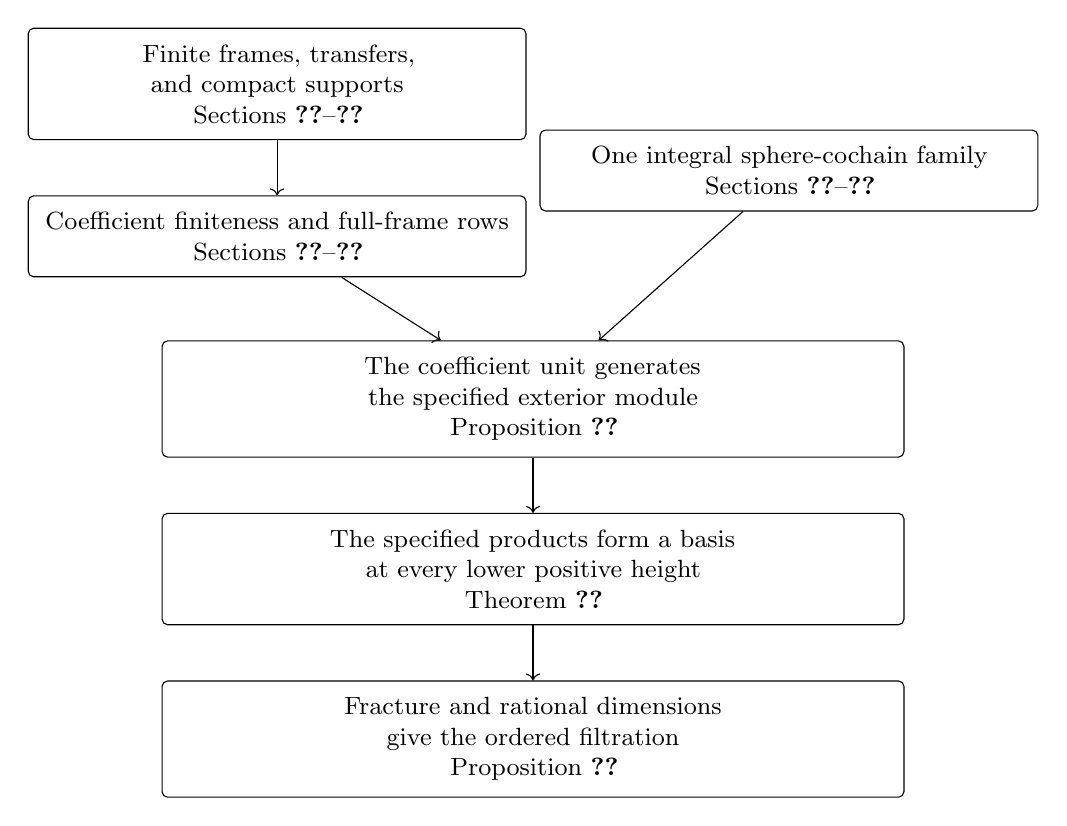
\begin{tikzpicture}[
  every node/.style={align=center,font=\small},
  box/.style={draw,rounded corners=2pt,inner sep=6pt,text width=5.9cm}
]
\node[box] (geometry) at (-3.25,0)
  {Finite frames, transfers, and compact supports\\
   Sections~\ref{sec:rings}--\ref{sec:support}};
\node[box,anchor=north] (finiteness)
  at ([yshift=-7mm]geometry.south)
  {Coefficient finiteness and full-frame rows\\
   Sections~\ref{sec:compact}--\ref{full:section}};
\node[box] (classes) at (3.25,-1.1)
  {One integral sphere-cochain family\\
   Sections~\ref{sec:constants}--\ref{sec:generators}};
\node[box,text width=9cm,anchor=north] (module)
  at ([xshift=3.25cm,yshift=-8mm]finiteness.south)
  {The coefficient unit generates\\the specified exterior module\\
   Proposition~\ref{prop:constant-module}};
\node[box,text width=9cm,anchor=north] (bases)
  at ([yshift=-7mm]module.south)
  {The specified products form a basis\\at every lower positive height\\
   Theorem~\ref{thm:height-bases}};
\node[box,text width=9cm,anchor=north] (filtration)
  at ([yshift=-7mm]bases.south)
  {Fracture and rational dimensions\\give the ordered filtration\\
   Proposition~\ref{prop:assembly}};
\draw[->] (geometry) -- (finiteness);
\draw[->] (finiteness) -- (module);
\draw[->] (classes) -- (module);
\draw[->] (module) -- (bases);
\draw[->] (bases) -- (filtration);
\end{tikzpicture}
\caption{The two inputs to the prescribed product bases. The left
branch keeps the algebraic coefficient topology and its constant-cochain
action; the right constructs the classes that act. Ordinary residue
descent recognizes their products, and the independent rational
calculation supplies the last filtration block.}
\label{fig:proof-architecture}
\end{figure}

\subsection{History and the ingredients of the proof}

Hopkins' chromatic splitting conjecture, recorded by Hovey
\cite[Conjecture~4.2]{Hovey}, proposes classes, factorizations, and a
splitting of a canonical cofiber sequence. Its weak consequence asks
for a retraction of the canonical unit comparison \cite[p.~2]{Hovey}. Barthel and
Beaudry review a revised strong formulation
\cite[Conjecture~6.3 and Remark~6.4]{BB}. The exterior-indexed
summand pattern motivates \eqref{eq:pieces}; Theorem~\ref{thm:main}
realizes that pattern as the successive cofibers of an ordered filtration
in the stated prime range.

Hovey's July 1993 account records the height-one case and the
height-two case at \(p>3\) as known, attributing the latter to Hopkins using
Shimomura--Yabe \cite[pp.~17--19]{Hovey}. Goerss--Henn--Mahowald
prove the height-two splitting at \(p=3\)
\cite[Theorem~1.2]{GHM2014}. At height two and prime two, Beaudry
disproved the original strong formula
\cite[Theorem~1.4]{Beaudry2017}. Beaudry--Goerss--Henn's
corrected calculation has additional Moore-spectrum terms and retains
a split unit \cite[Theorem~1.1.6]{BGH2022}.

Barthel--Schlank--Stapleton--Weinstein determine the rational
homotopy of the \(K(n)\)-local sphere at every positive height and
prime \cite[Theorem~A]{BSSW}. Their result gives
\begin{equation}\label{eq:rational-dimensions}
 \dim_{\Qp}\pi_{-b}L_0D
  =\#\{I\subseteq\{1,\ldots,n\}:d(I)=b\}.
\end{equation}
This determines the size of the last, rational block. It does not
identify the maps in \eqref{eq:height-basis}. We do not identify its
individual rational generators with our integral \(y_i\).

Torii developed common-coefficient comparisons between adjacent
Morava theories and the localized descent spectral sequences they
induce, including the unit comparison and survival of the reduced-norm
class \cite[Theorems~4.7, 6.2, 7.6, and~8.1]{ToriiTranschromatic}.
The characteristic-\(p\) period domains of
Barthel--Mann--Ray--Schlank--Senger--Weinstein--Zhou provide a geometric
approach to the coheight-one problem. For \(n\geq2\), their
Corollary~B shows that the map
\[
L_{K(n-1)}S\ \vee\ \Sigma^{-1}L_{K(n-1)}S
       \longrightarrow L_{K(n-1)}D
\]
represented by the unit and the Devinatz--Hopkins class admits a
retraction when \((p-1)\nmid(n-1)\). Their Theorem~C gives the
full equivalence at height two and odd primes \cite{BMR}.
Their relative two-tower description also identifies the determinant
normalization for positive-height strata
\cite[Theorems~2.0.1 and~2.6.3]{BMR}.

The coefficient distinction emphasized in \cite[Section~1.5]{BMR}
is essential here. At intermediate heights \(0<t<n-1\), analytic
functions on the punctured stratum form a larger ring than the
arithmetic coefficients arising from ordinary chromatic base change.
Our height test requires the algebraic union
\(\mathcal B_{n,t}\) with its common finite-stage and bounded-pole
cochains. Sections~\ref{sec:support}--\ref{full:section} connect its
cohomology to integral compact supports through transfer and the
boundary induction, while retaining that algebraic coefficient
convention.

To connect the finite frame tower to integral compact supports, we
pass from torsion coordinates to bundle extensions and track the transfer
system. Hopkins and Gross relate the rigid generic Lubin--Tate deformation
space to projective geometry through an equivariant period map
\cite[Theorem~1]{HopkinsGross1994}.
The finite torsion-coordinate calculation is closely related to
Strauch's analysis of universal formal modules \cite{Strauch};
the exact-height connected markings use the formal-group
classification in \cite[Lecture~14, Theorem~1]{LurieFormalGroups}.
The passage to bundles uses the Fargues--Fontaine curve
\cite{FarguesFontaine}, the universal-cover description of
Scholze--Weinstein \cite{ScholzeWeinstein}, the relative slope
classification of Fargues--Scholze \cite{FarguesScholze}, and the
full faithfulness for positive section sheaves of
Ansch\"utz--Le Bras \cite{AnschuetzLeBrasFourier}. Primitive comparison
and open--closed localization for integral coefficients supply the
geometric comparisons \cite{ScholzeHodge,PignonYwanne}.
The compact-parameter and incidence arguments in
Section~\ref{sec:support} establish the uniformity required to apply
these comparisons to the finite marking tower and its transfers.

To obtain one family of acting sphere classes, we compare constant
cochains and construct stable representatives with integral product
normalization. Dotto--Le Hung compute the required mod-\(p\) constant
cohomology in the range \(a<p-1\) \cite{DLH}; the integral deduction
is included in Section~\ref{sec:constants}. The same section uses
the integral Drinfeld-space calculation of
Colmez--Dospinescu--Nizio\l\ \cite{CDN} to compare constant cochains
through a common modification space. The construction of stable
representatives then uses the continuity theorem of
Geisser--Hesselholt \cite{GeisserHesselholt}, in the modern formulation
of Clausen--Mathew--Morrow \cite{CMM}, the local cyclotomic-trace
comparison of Hesselholt--Madsen \cite{HesselholtMadsenWitt}, and the
chosen coordinates in topological cyclic homology of
Blumberg--Mandell \cite{BlumbergMandellTC}. The regulator comparison of Huber--Kings
\cite{HuberKings} and the suspended-Chern volume calculation of
Huber--Soergel \cite{HuberSoergel} supply the rational normalization
data. Section~\ref{sec:generators} combines them with local lattice and
sphere-lifting arguments to obtain the integral normalization needed
for the products to remain generators modulo \(p\).

\section{A criterion for the filtration}
\label{sec:assembly}

We first isolate the passage from compatible local bases to an actual
filtration. The construction removes the basis maps in blocks, ordered
by the largest index in their subsets. Each block kills the highest
remaining chromatic layer of the quotient. After the last positive
height has been removed, rational independence determines the remaining
block. Taking fibers of the quotient maps then recovers a filtration
of the original object. The same maps must serve as bases at every
height so that removing an earlier block has this prescribed effect
on every later test.

\subsection{Localizations and scalar conventions}

Fix a prime \(p\), and write \(S=S_p^\wedge\). We work in the stable
category of \(S\)-modules. Localizations are detected on the underlying
spectra. In particular, an \(S\)-module is \(E(r)\)-local or
\(K(t)\)-local when its underlying spectrum is so. These localizations
inherit their \(S\)-module structure and adjunction from the monoidal
Bousfield localization of spectra. All the fibers and cofibers below
are taken in \(S\)-modules.

We use three familiar consequences of chromatic localization:
\begin{enumerate}[label=(\roman*)]
\item If \(r\geq t\), the localization unit induces
\[
 L_{K(t)}S \xrightarrow{\;\simeq\;} L_{K(t)}L_rS.
\]
\item If an \(E(t)\)-local object \(Q\) satisfies \(L_{K(t)}Q=0\),
then \(Q\) is \(E(t-1)\)-local. This is the chromatic fracture square
applied to \(Q\).
\item \(L_0L_rS=L_0S=H\Qp\) for every \(r\geq0\).
Consequently rational \(S\)-modules are modules over \(H\Qp\).
\end{enumerate}
The first statement follows because every \(E(r)\)-equivalence is a
\(K(t)\)-equivalence. Composing localizations gives the first equality
in (iii): rationalization is already an \(E(r)\)-localization of lower
height. To identify its value, let \(\mathbb S\) denote the sphere before
completion. Its positive stable stems are finite: choose an odd sphere
in the stable range and apply Serre's finiteness theorem
\cite[Chapter~V, Section~3, Proposition~3]{Serre1951}.
The Moore exact sequences for \(\mathbb S/p^v\) and the Milnor sequence
for their inverse limit then give
\[
\pi_0S=\Zp,\qquad
\pi_iS=(\pi_i\mathbb S)^{\wedge}_p\quad(i>0),\qquad
\pi_iS=0\quad(i<0).
\]
Indeed, the finite Moore groups satisfy Mittag--Leffler, and the
transition on the torsion kernels in the Moore exact sequences is
multiplication by \(p\), so their inverse limit is zero. Thus the
positive groups displayed above are finite \(p\)-groups. Rationalizing
leaves only \(\Q\otimes\Zp=\Qp\) in degree zero, proving \(L_0S=H\Qp\).
The standard fracture square and these localization conventions are
reviewed in \cite[Section~2]{BB}.

We will also use that the unit of \(L_{K(1)}S\) is nonzero after
rationalization. At odd \(p\), height-one Morava theory is
\(E_1\simeq KU_p^\wedge\), with \(\Zp^\times\) acting through
Adams operations. The structured homotopy fixed point spectral sequence
\[
H_c^s(\Zp^\times;\pi_rE_1)
\Longrightarrow \pi_{r-s}L_{K(1)}S
\]
is strongly convergent
\cite[Theorem~1(iii)--(iv) and pp.~2--3]{DevinatzHopkins}.
The \(p\)-cohomological dimension of
\(\Zp^\times=\mu_{p-1}\times(1+p\Zp)\) is one. Since
\(\pi_*E_1\) is even and the action on \(\pi_0E_1=\Zp\) is
trivial, total degree zero has only the term
\(H_c^0(\Zp^\times;\pi_0E_1)=\Zp\). The augmentation sends the
actual sphere unit to \(1\) on this edge. Hence
\(\pi_0L_{K(1)}S\cong\Zp\), with the unit corresponding to \(1\);
its rationalization is nonzero.

\subsection{The simultaneous basis criterion}

For a finite subset \(I\) of the positive integers put
\[
d(I)=\sum_{i\in I}(2i-1),\qquad d(\varnothing)=0.
\]
When we refer to a map representing an element of
\(\pi_{-d(I)}D\), its source is the free \(S\)-module
\(\Sigma^{-d(I)}S\).

\begin{proposition}[Filtration criterion]
\label{prop:assembly}
Let \(n\geq1\), let \(p\) be odd, and let \(D\) be an \(S\)-module with
a specified map \(u:S\to D\). Suppose that maps
\[
z_I:\Sigma^{-d(I)}S\longrightarrow D,
\qquad I\subseteq\{1,\ldots,n-1\},
\qquad z_\varnothing=u,
\]
have the following properties.
\begin{enumerate}[label=(\alph*)]
\item For each \(1\leq t<n\), the map with the specified components
\begin{equation}
\bigvee_{I\subseteq\{1,\ldots,n-t\}}\Sigma^{-d(I)}S
 \xrightarrow{(z_I)} D
\label{eq:criterion-bases}
\end{equation}
is a \(K(t)\)-equivalence.
\item For every integer \(b\),
\begin{equation}
\dim_{\Qp}\pi_{-b}L_0D
=\#\{I\subseteq\{1,\ldots,n\}:d(I)=b\}.
\label{eq:criterion-rational}
\end{equation}
If \(n=1\), assume in addition that \(\pi_0L_0u\) is nonzero.
\end{enumerate}
Then \(X=L_{n-1}D\) has the filtration and unit compatibility of
Theorem~\ref{thm:main}(a), with \(u\) in place of its unit.
\end{proposition}

\begin{proof}
First suppose \(n>1\). We construct successive quotients \(Q_j\) of
\(X\), starting with \(Q_0=X\). The first block is
\[
B_1=L_{n-1}S\ \vee\ \Sigma^{-1}L_{n-1}S.
\]
Localizing the maps \(z_\varnothing,z_{\{1\}}\) gives a map
\(B_1\to Q_0\). Let \(Q_1\) be its cofiber. Applying
\(L_{K(n-1)}\), hypothesis~(a) identifies this map with an
equivalence. The cofiber \(Q_1\) is therefore \(E(n-2)\)-local.

Inductively, assume that \(2\leq j\leq n-1\) and that \(Q_{j-1}\)
is \(E(n-j)\)-local. For every \(I\) with \(\max I=j\), compose
\(z_I\) with \(D\to X\to Q_{j-1}\). The localization adjunction
extends this map uniquely, in the space of such extensions, to
\(\Sigma^{-d(I)}L_{n-j}S\). We thus obtain
\begin{equation}
B_j=\bigvee_{\max I=j}\Sigma^{-d(I)}L_{n-j}S
 \longrightarrow Q_{j-1}\longrightarrow Q_j,
\label{eq:block-quotient}
\end{equation}
where the last object is the cofiber.

Here is the compatibility needed to continue the induction. Fix
\(t=n-j\). Hypothesis~(a) gives a specified direct-sum basis of
\(L_{K(t)}D=L_{K(t)}X\), indexed by the subsets of
\(\{1,\ldots,j\}\). For each earlier block \(\ell<j\), its sphere
localization has height at least \(t\). Its \(K(t)\)-localization is
therefore the corresponding shift of \(L_{K(t)}S\), and its map is
the image of the original component \(z_I\). Successive cofibers
of these components remove exactly the subsets whose maximum is
less than \(j\), together with the empty subset. This assertion is
inductive: at each step the map into the cofiber is the composite
of that same original component with the quotient map, so the
cofiber is the quotient by that direct summand.

The remaining summands are precisely the components of \(B_j\).
It follows that \(L_{K(t)}(B_j\to Q_{j-1})\) is an equivalence.
Consequently \(L_{K(t)}Q_j=0\), and chromatic fracture makes
\(Q_j\) \(E(t-1)\)-local. The construction thus reaches a rational
object \(Q_{n-1}\). For \(n=2\), this is already the object \(Q_1\)
constructed from the first block.

We next determine that rational quotient, keeping track of possible
kernels. The elements
\[
z_I,\qquad I\subseteq\{1,\ldots,n-1\},
\]
are linearly independent after rationalization in each degree.
Indeed, under hypothesis~(a) at \(t=1\), their images in
\(L_{K(1)}D\) are the units of distinct shifted summands
\(\Sigma^{-d(I)}L_{K(1)}S\). The rationalized unit in each such
summand is nonzero. A rational relation between the \(z_I\) would
therefore give a relation between nonzero elements in different
summands, which is impossible. This argument includes subsets
with equal values of \(d(I)\).

Since \(L_0L_rS=H\Qp\), rationalizing the map from each block
gives, in every degree, the injection of the corresponding
independent vectors into the quotient by the preceding vectors.
The cofiber long exact sequence has no suspended kernel. Subtracting
these vectors from the dimensions in hypothesis~(b) leaves
\[
\dim_{\Qp}\pi_{-b}Q_{n-1}
=\#\{I\subseteq\{1,\ldots,n\}:\max I=n,\ d(I)=b\}.
\]
The derived category of \(\Qp\)-vector spaces splits by homology.
Choose a basis in each degree to obtain an equivalence of
rational \(S\)-modules
\[
B_n=\bigvee_{\max I=n}\Sigma^{-d(I)}H\Qp
 \xrightarrow{\;\simeq\;}Q_{n-1}.
\]
Its cofiber \(Q_n\) is zero.

It remains to pass from these successive quotients to a filtration
of \(X\). Set
\[
G_j=\fib(X\longrightarrow Q_j),\qquad 0\leq j\leq n.
\]
Then \(G_0=0\) and \(G_n=X\). For each block the square
\begin{equation}
\begin{tikzcd}
G_j \arrow[r] \arrow[d] & B_j \arrow[d]\\
X \arrow[r] & Q_{j-1}
\end{tikzcd}
\label{eq:filtration-pullback}
\end{equation}
is cartesian: its upper left corner is the fiber of
\(X\to Q_j=\cofib(B_j\to Q_{j-1})\). Taking fibers of its horizontal
maps yields the cofiber sequence
\[
G_{j-1}\longrightarrow G_j\longrightarrow B_j.
\]
If a block is \(B_j=C_1\vee\cdots\vee C_r\), replace \(G_j\) by
the intermediate pullbacks along
\[
0\longrightarrow C_1\longrightarrow C_1\vee C_2
\longrightarrow\cdots\longrightarrow B_j.
\]
Exactness of pullback in a stable category makes their successive
cofibers \(C_1,\ldots,C_r\). In the first block choose the unit
summand first. Its pullback identifies the first stage with
\(L_{n-1}S\), and its map to \(X\) is exactly the localized \(u\).
The other blocks are already ordered by maximum. The number of
individual pieces is
\[
2+\sum_{j=2}^{n-1}2^{j-1}+2^{n-1}=2^n.
\]
This constructs the required filtration by \(S\)-linear maps.

If \(n=1\), the object \(X=L_0D\) is rational. Hypothesis~(b)
places one copy of \(\Qp\) in degree zero and one in degree
\(-1\). The nonzero map \(L_0u:H\Qp\to X\) is an isomorphism on
degree-zero homotopy, so its cofiber is
\(\Sigma^{-1}H\Qp\). These are the two required stages.
\end{proof}

\begin{remark}
\label{rem:assembly-extensions}
The construction uses maps into the current quotient. Diagram
\eqref{eq:filtration-pullback} retains their boundary maps when
the blocks are pulled back to \(X\). Thus the criterion produces
the attaching maps as part of the filtration; it requires no
choice of a nullhomotopy for them.
\end{remark}

\section{Finite frame rings and Cartier transfers}
\label{sec:rings}

To compare coefficient cohomology with compact supports, we need transfers
whose transpose is the actual Frobenius on functions of the finite covers. This
section constructs the finite frame rings and lift torsors, then normalizes
their Cartier transfers to obtain that map in Lemma~\ref{lem:cartier-transfer}.

Fix integers $1\leq t<n<p-1$, and put $m=n-t$.  Choose a finite
field $k$ containing the fields of definition of the Honda endomorphisms
at the heights at most $n$.  Its degree over $\Fp$ may be chosen prime
to $p$: a multiple of $\operatorname{lcm}(1,\ldots,n)$ suffices for
these endomorphism fields.  Further finite extensions used below are
chosen with the same property.  Write
\[
 A=k[[x_t,\ldots,x_{n-1}]],\qquad x=x_t,\qquad B=A[1/x].
\]
Here $A$ is the height-$t$ quotient of the characteristic-$p$
Lubin--Tate deformation ring of the height-$n$ Honda group.  Write
$\mathcal G_A$ for its formal group and
$P_n=\mathcal O_{D_n}^{\times}$ for the ordinary height-$n$
stabilizer.  The action on a function induced by a left action on
points is always inverse substitution.

We choose a coordinate on $\mathcal G_A$ lifting the fixed Honda
coordinate and having the height congruences
\begin{equation}\label{rings:height-congruences}
 [p](T)\equiv x_iT^{p^i}
 \pmod{(x_t,\ldots,x_{i-1},T^{p^i+1})},
 \qquad t\leq i\leq n,
 \quad x_n=1.
\end{equation}
The same choice gives the full special-fiber identity
\[
 [p](T)\equiv T^{p^n}\pmod{(x_t,\ldots,x_{n-1})}
\]
as an identity of formal series.  Moreover $[p](T)$ factors through
$T^{p^t}$ over $A$.
The group used on $B$ is the algebraic $p$-divisible group obtained
from the finite kernels over $A$.  More explicitly, Weierstrass
preparation makes
\[
 A[[T]]/([p^l](T))
\]
a finite free $A$-algebra of rank $p^{nl}$.  Its torsion coordinate is
topologically nilpotent before localization, so the formal addition
and multiplication series define algebraic group operations on this
finite algebra.  Preparation for $[p](T)-Z$ gives the finite flat
transition maps.  We localize these finite group schemes at $x$.
Thus the connected--\'etale sequence on $B$ retains the entire finite
kernel, including its infinitesimal connected part.

\subsection{Labeled rings before localization}

For $l\geq1$, consider $m$ points of $\mathcal G_A[p^l]$ whose
images form a basis of the \'etale quotient at the generic point of
$A$.  Let $\widetilde C_l$ be the reduced closure of this generic
lifted-basis locus in the finite scheme of $m$ torsion points, and
write $z_{1,l},\ldots,z_{m,l}$ for the lifted coordinates.  Set
\[
 w_{i,l}=z_{i,l}^{p^{tl}},\qquad
 C_l=A[w_{1,l},\ldots,w_{m,l}]\subseteq\widetilde C_l.
\]
These finite $A$-algebras are complete.  A reduced closure is used
only to establish their coordinates; the proposition also identifies
the unreduced scheme that will be used for descent.
For the boundary convention $t=n$, the empty labeled ring is $k$.

\begin{proposition}[Finite labeled rings]\label{prop:finite-rings}
There are compatible identifications
\begin{equation}\label{rings:regular-coordinates}
 C_l=k[[w_{1,l},\ldots,w_{m,l}]],\qquad
 \widetilde C_l=k[[z_{1,l},\ldots,z_{m,l}]],\qquad
 w_{i,l}=z_{i,l}^{p^{tl}}.
\end{equation}
Both rings are finite free over $A$.  On the exact-height locus,
$C_l[1/x]$ is the finite \'etale algebra of bases of the \'etale
$p^l$-torsion.  Over this algebra the scheme of all lifts of its
universal basis to $\mathcal G_A[p^l]$ has algebra
\[
 \widetilde C_l[1/x]=(C_l[1/x])^{1/p^{tl}},
\]
finite locally free of rank $p^{tlm}$.

The transition maps are finite and injective, and for $j\leq l$
\begin{equation}\label{rings:transition-powers}
 z_{i,j}\in
 k[[z_{1,l}^{p^{t(l-j)}},\ldots,z_{m,l}^{p^{t(l-j)}}]].
\end{equation}
\end{proposition}

\begin{proof}
The algebra $\widetilde C_l$ is finite and reduced, and each of its
irreducible components dominates $\Spec A$ by its definition as a
generic closure.  It has dimension $m$.  Above the closed point of
$A$ all torsion coordinates are nilpotent, so there is a unique
closed point and its residue field is $k$.  Its maximal ideal is
generated by the height parameters and the $z_{i,l}$.

Put $a_i=[p^{l-1}](z_{i,l})$, and for $v\in\Fp^m$ let $a_v$ be
the corresponding formal-group linear combination of the $a_i$.
If $W_p(T)$ is the distinguished polynomial for $[p](T)$, then
\begin{equation}\label{rings:basis-polynomial}
 W_p(T)=\prod_{v\in\Fp^m}(T-a_v)^{p^t}
       =\prod_{v\in\Fp^m}(T^{p^t}-a_v^{p^t}).
\end{equation}
Indeed this is the factorization over every geometric generic
field: the distinct \'etale points are indexed by the labels and
each has connected multiplicity $p^t$.  Both sides are monic of
degree $p^n$, so generic density in the reduced algebra proves the
identity there.

There is a series $h_l$ with
$[p^{l-1}](T)=h_l(T^{p^{t(l-1)}})$.  Consequently
$a_i^{p^t}$ is a power series in $w_{i,l}$ with coefficients in
$A$ and zero constant term.  Taking formal-group linear
combinations gives the same assertion for every $a_v^{p^t}$.
Thus \eqref{rings:basis-polynomial} is an identity over $C_l$,
and modulo $(w_{1,l},\ldots,w_{m,l})$ it becomes $T^{p^n}$.
The preparation unit for $[p](T)$ is defined over $A$.  All
coefficients of $[p](T)$ of degree below $p^n$ therefore vanish in this
quotient, and \eqref{rings:height-congruences} successively gives
\[
 x_t=x_{t+1}=\cdots=x_{n-1}=0.
\]
The maximal ideal of $C_l$ is generated by its $m$ displayed
$w$-coordinates.  Since $C_l$ is integral over $A$, its dimension
is $m$.  It is a regular local ring, and the surjection from
$k[[W_1,\ldots,W_m]]$ taking $W_i$ to $w_{i,l}$ is an
isomorphism: a nonzero kernel would lower the dimension of this
power-series domain.  The identical maximal-ideal argument with
the $z_{i,l}$ gives the second identification in
\eqref{rings:regular-coordinates}, including the stated
inclusion.  These finite regular rings are Cohen--Macaulay of
dimension $m$; the parameters of $A$ form systems of parameters
on them.  Their Koszul complexes are exact in positive degree,
so the finite modules are flat, hence free, over the local ring
$A$.

We next check the finite schemes after localization.  Write
\[
 [p^l](T)=g_l(T^{p^{tl}}),\qquad
 g_l(S)=U_l(S)V_l(S),
\]
where $U_l$ is a unit and $V_l$ is distinguished of degree
$p^{ml}$.  The linear coefficient of $g_l$ is a unit times
$x^{1+p^t+\cdots+p^{t(l-1)}}$.  The invariant-differential
identity for this Frobenius-divided homomorphism expresses
$g_l'(S)$ as that coefficient times a quotient of unit series.
Evaluating in the prepared finite algebra shows that $V_l'$ is
a unit after $x$ is inverted.  Thus the Frobenius-divided finite
group is \'etale there, of rank $p^{ml}$.  Its kernel quotient
has removed exactly the connected kernel of rank $p^{tl}$.

The scheme of bases of this \'etale group is finite \'etale over
$B$.  The universal labeled points give a surjection from its
algebra to $C_l[1/x]$.  It is an isomorphism generically, since
the generic closure included every basis.  Its kernel is zero:
the source is flat over the domain $B$, whereas a kernel
vanishing generically would be $B$-torsion.  This identifies the
basis algebra.

Over this basis algebra, the scheme of lifts of the $m$ basis
vectors is a product of torsors for the connected finite kernel.
It is finite locally free of rank $p^{tlm}$.  Its algebra
surjects onto $\widetilde C_l[1/x]$, which is generated by the
same lifted coordinates.  The latter is free over $C_l[1/x]$
with basis
\[
 \prod_{i=1}^m z_{i,l}^{e_i},\qquad 0\leq e_i<p^{tl}.
\]
The two ranks are equal, so the surjection is an isomorphism.
This is the assertion about the full lift scheme, rather than
its reduction.

A basis at level $j$ lifts to a basis at level $l$ over an
extension of every geometric generic field.  Hence the
transition maps on the reduced closures are injective.  They
are finite because both rings are finite over $A$.  Since
$z_{i,j}=[p^{l-j}](z_{i,l})$, factorization through Frobenius
and \eqref{rings:regular-coordinates} give
\eqref{rings:transition-powers}.

\end{proof}

The underlying regular-quotient and \'etale-coordinate
construction is also described at arbitrary height in
\cite[\S\S3--4, Proposition~4.1]{Strauch}.  The explicit
rank comparison above records the additional finite-flat
statement needed for our translation torsors.

The boundary calculation also needs a presentation that survives
nilpotent base change.  We establish that presentation before
identifying the locus on which a label vanishes.

\begin{lemma}[An integral full-section presentation]
\label{rings:full-sections-presentation}
Let $H$ be the quotient of $\mathcal G_A[p]$ by its relative
$p^t$-Frobenius kernel.  The ring $C_1$ represents full labeled
section tuples $\Fp^m\to H$, including over nilpotent test
rings.  Here ``full'' means equality of the finite Cartier
divisors, or equivalently, after every base change,
equality of the norm of every function with its product
over the labeled sections.
\end{lemma}

\begin{proof}
The quotient $H$ has the monogenic presentation obtained by
dividing the prepared $p$-series by relative Frobenius.  The
full-section condition is a finite set of coefficient
identities for its monic polynomial.  Indeed equality for the
coordinate implies equality of the characteristic polynomial
for every polynomial in that coordinate by substitution, and
every function in the finite algebra has such a representative.
This description commutes with arbitrary base change.

Let $Q$ be the resulting finite complete $A$-algebra of labeled
group-homomorphism tuples.  It has one closed point, because
at the closed point of $A$ the connected finite group has only
the zero section over a field.  If all $m$ labeled coordinates
are set equal to zero, the full-section identity makes the
divided distinguished polynomial $T^{p^m}$.  Applying
\eqref{rings:height-congruences} before this division
successively kills all the height parameters.  Thus the
maximal ideal of $Q$ has at most $m$ generators.  There is a
surjection $Q\twoheadrightarrow C_1$ induced by the generic
full tuple.  Since $C_1$ has dimension $m$, the dimension and
embedding dimension of $Q$ are both $m$.  Hence $Q$ is regular.
A quotient of this regular local domain of the same dimension
has zero kernel, proving $Q=C_1$.

All equations in this argument are equations in finite
algebras formed before localization.  Their subsequent use
on an \'etale component therefore involves polynomial
operations in a finite algebra; it does not require substituting
an order-one element into an unevaluated formal series.
\end{proof}

\begin{corollary}[Vanishing labels and higher starting height]
\label{rings:boundary-labels}
At level one, for each nonzero label $v\in\Fp^m$ there is a
coordinate $w_v$ such that
\begin{equation}\label{rings:height-divisor}
 x=\text{a unit}\cdot\prod_{0\ne v\in\Fp^m}w_v.
\end{equation}
Each ideal $(w_v)$ is $P_n$-stable.  Its conormal is a power of the
invariant coordinate line.  For a primitive label, the quotient by
$(w_v)$ is the starting-height-$(t+1)$ level-one ring with $p$-th
roots of its parameters adjoined.  The same assertion can be
iterated for any independent set of dead labels.
\end{corollary}

\begin{proof}
At level one let $a_v$ be the formal-group linear combination of
$z_{1,1},\ldots,z_{m,1}$ with label $v\in\Fp^m$, and put
$w_v=a_v^{p^t}$.  The coefficient of $T^{p^t}$
in \eqref{rings:basis-polynomial}, together with the
preparation unit, gives \eqref{rings:height-divisor}.
Transport by $P_n$ is a change of formal coordinate with
invertible linear coefficient.  Its action on $w_v$ is $w_v$
times a unit, proving stability of $(w_v)$.  On the conormal
only that linear coefficient remains, raised to the $p^t$-th
power.  Equivalently, this is the invariant cotangent line of
the Frobenius-divided group restricted to its zero section.
This also describes the action without a choice of generator
for the line.

Change the labels so that $v$ is the first basis vector, and
put $R=C_1/(w_1)=k[[w_2,\ldots,w_m]]$.
Write $[p](T)=g_t(T^{p^t})$ and let $Q_t$ be the distinguished
polynomial of $g_t$.  Formula~\eqref{rings:height-divisor}
gives $x_t=0$ in $R$.  The labels in each coset of $\Fp v$
then give the same point, so
\[
 Q_t(Y)=\prod_{\bar v\in\Fp^{m-1}}
              (Y^p-w_{\bar v}^{p}).
\]
Over $A/(x_t)$ we have $g_t(Y)=g_{t+1}(Y^p)$, and uniqueness
of preparation gives $Q_t(Y)=Q_{t+1}(Y^p)$.  Therefore
\[
 Q_{t+1}(Z)=\prod_{\bar v\in\Fp^{m-1}}(Z-w_{\bar v}^p).
\]
Coefficient Frobenius identifies these labels with the
formal-group combinations of $w_2^p,\ldots,w_m^p$ in the
next Frobenius twist.  By Lemma~\ref{rings:full-sections-presentation},
the displayed full-section identity gives a map from the
starting-height-$(t+1)$ labeled ring, whose labeled
coordinates map to $w_2^p,\ldots,w_m^p$.
In the power-series coordinates of
Proposition~\ref{prop:finite-rings}, this map is injective with image
$k[[w_2^p,\ldots,w_m^p]]=R^p$, since $k$ is perfect.
Thus $R$ is exactly its $p$-th-root extension, with the
indicated $A/(x_t)$-structure.  Repeating the calculation
for $h$ independent dead labels sends the higher-height
labeled coordinates to $w_{h+i}^{p^h}$ and gives the corresponding
$p^h$-th-root extension.
\end{proof}

\subsection{Connected markings and compatible lifts}

Let $\Gamma_t$ be the height-$t$ Honda group over $k$.
A connected marking is an isomorphism
\[
 \alpha:\Gamma_t\longrightarrow \mathcal G_B^0
\]
of formal groups, and an \'etale marking is an integral basis
$i:\Zp^m\longrightarrow T_p\mathcal G_B^{\mathrm{et}}$.
Their joint algebraic tower has structure group
\[
 U_0=P_t\times\GL_m(\Zp),\qquad
 P_t=\mathcal O_{D_t}^{\times}.
\]
We use the left action
$(h,a)(\alpha,i)=(\alpha h^{-1},ia^{-1})$.
For an open subgroup $U\subseteq U_0$, write $B_U$ for the
corresponding finite frame algebra.  Write
$\mathcal B=\colim_U B_U$ for the entire joint algebraic
frame ring.  No completion of this union is part of this
notation.

\begin{proposition}[Frame and lift torsors]\label{prop:frame-torsor}
The rings $B_U$ form a tower of finite \'etale $B$-algebras.
After passing to normal open levels, the maps in the tower
are finite \'etale torsors for the indicated finite deck
groups.  The tower is $P_n$-equivariant, and $P_n$ commutes
with its $U_0$-action.

Over $\mathcal B$, the scheme of lifts of the compatible
\'etale basis is an affine faithfully flat torsor for
\begin{equation}\label{rings:translation-group}
 T=(T_p\Gamma_t)^m,
 \qquad
 T_p\Gamma_t=\varprojlim_{[p]}\Gamma_t[p^r].
\end{equation}
For every $r\geq1$ its finite quotient has group
$T/[p]^rT=\Gamma_t[p^r]^m$ and algebra
\begin{equation}\label{rings:root-torsor}
 \mathcal B^{1/p^{tr}}.
\end{equation}
Thus the full lift algebra is the algebraic root union
$\mathcal B^{\mathrm{perf}}$.
The group $P_n$ acts trivially on the translation parameters.
The action of $(h,a)\in U_0$ on a translation tuple $\tau$ is
\begin{equation}\label{rings:auxiliary-action}
 \tau\longmapsto h\tau a^{-1}.
\end{equation}
All finite torsor constructions and all their morphisms
descend to finite frame levels once their finite marking
data are included.
\end{proposition}

\begin{proof}
Over $B$ the lower height coefficients vanish and the
height-$t$ coefficient is invertible.  The full isomorphism
ring between this law and $\Gamma_t$ is therefore a filtered
union of finite \'etale extensions, by the exact-height
isomorphism theorem \cite[Lecture~14, Theorem~1]{LurieFormalGroups}.
For clarity, its finite stages record coefficients of a full
isomorphism that extend to the next required equations.
The first coefficient $c$ satisfies
$c^{p^t-1}=x^{-1}$ up to the chosen leading unit.  The
subsequent free coefficients satisfy monic additive equations
with invertible linear coefficient; the other coefficients
are uniquely determined.  The equation constraining a
coefficient of degree $p^j$ can occur at degree $p^{t+j}$.
Thus these are not the schemes of arbitrary finite-bud
isomorphisms.  Any two full markings differ uniquely by
$P_t$, and quotienting by an open subgroup gives its finite
\'etale torsor stages.

The \'etale Tate basis tower is finite \'etale at each
level, as proved in Proposition~\ref{prop:finite-rings}.
Taking the product of the two frame torsors proves the
first assertion.  Universal deformation transport carries
both markings along the same isomorphism; it commutes with
changing the markings.  This proves the asserted $P_n$
equivariance.

At finite level $r$, two lifts of the marked \'etale basis
differ by exactly one element of $\Gamma_t[p^r]^m$.
Proposition~\ref{prop:finite-rings} identifies the lift
algebra over the \'etale basis cover with its $p^{tr}$-th
root ring.  Relative Frobenius commutes with finite \'etale
base change, so the same identification holds after any
connected marking base change.  It is canonical: each
element of the lift algebra is the unique $p^{tr}$-th root
of its power in the base.  The identity may be checked on
the faithfully flat basis cover and then descended.

The finite torsor maps are faithfully flat and the
transition on lifts is multiplication by $p$.  Taking
their affine inverse limit gives the torsor identity and
faithful flatness for \eqref{rings:translation-group}.
The kernel of the projection $T\to\Gamma_t[p^r]^m$ is
$[p]^rT$: shifting a compatible sequence by $r$ constructs
its unique preimage under $[p]^r$.  This proves both the
subgroup assertion and \eqref{rings:root-torsor}.

Finally, transport by $P_n$ carries the connected marking,
the \'etale basis, and its lift simultaneously, so it fixes
their difference parameter in the constant Honda group.
Changing the markings by $(h,a)$ instead changes that
parameter by \eqref{rings:auxiliary-action}.  Each finite
kernel and each finite diagram uses finitely many
coefficients of the connected marking and a finite
\'etale level, proving finite-stage descent.
\end{proof}

\Needspace{8\baselineskip}
\begin{definition}[Coefficient and cochain convention]
\label{rings:bounded-cochains}
For a finite projective module over a finite frame algebra
we use continuous cochains with bounded poles.  On a compact
profinite source this means that one power of $x$ places the
entire image in a finite power-series lattice, where the
cochain is continuous for the parameter-adic topology.
For a union of frame, root, or associated-bundle coefficients,
one common finite stage is required on each compact source.
Equivalently the cochain complex of such a union is the
filtered colimit of its finite-stage bounded-pole cochain
complexes.  These conventions also apply with an additional
compact profinite parameter.
\end{definition}

Finite free coordinate formulas, module splittings, and
finite \'etale descent preserve this convention.  A fixed
finite diagram can have a fixed pole loss, but its formulas
require only finitely many coefficients and denominators.
The compact-lattice estimates and continuous cochain
exactness used later will be established with these
coefficient topologies.

\subsection{The dual distribution ring}

The distribution ring organizes the translation representations at each
finite root level. Its identifications across Frobenius levels will be used in
Lemma~\ref{lem:cartier-transfer} to normalize the transfer and identify its
transpose with the actual Frobenius on cover functions.

Suppose first that $t>1$, and put $d=m(t-1)$.
The category of rational representations of the affine
group scheme $T$ is the category in which every vector
belongs to a representation of a finite quotient of $T$.
It is not the representation category of its geometric
points.  Finite Cartier duality identifies its completed
distribution ring with
\begin{equation}\label{rings:distribution-ring}
 \Lambda=\varprojlim_r\mathcal O(\Gamma_t[p^r]^m)^\vee
     =\mathcal O((\widehat{\Gamma_t^\vee})^m)
     \simeq k[[D_1,\ldots,D_d]].
\end{equation}
Here $(-)^\vee$ on a finite vector space is its $k$-linear
dual.  Rational representations correspond to discrete
modules locally killed by powers of the augmentation ideal.
The displayed parameters need not linearize the auxiliary
action.

\begin{lemma}[Divisible Frobenius levels]\label{rings:dual-distribution}
There is a positive integer $r_0$, divisible by $t-1$, such
that for $r=ar_0$, $a\geq1$, the two numbers
\begin{equation}\label{rings:two-frobenius-indices}
 Q=p^{tr},\qquad q=p^{tr/(t-1)}
\end{equation}
are Frobenius powers fixing $k$.  At this level
\[
 \mathcal O((\Gamma_t^\vee[p^r])^m)
   =\Lambda_q:=\Lambda/(D_1^q,\ldots,D_d^q),
 \qquad
 \dim_k\Lambda_q=q^d=Q^m.
\]
The embedding $[p]^r:T\hookrightarrow T$ corresponds on
distributions to
\[
 \psi_q:\Lambda\longrightarrow\Lambda,
 \qquad D_j\longmapsto D_j^q,\quad c\longmapsto c\ (c\in k).
\]
If $N_q=\mathcal O(T/[p]^rT)$ is the regular function
representation, finite Hopf duality gives a normalized
equivariant identification $N_q\simeq\Lambda_q$ as
translation representations.  The auxiliary action on
each finite quotient factors through a finite group.
\end{lemma}

\begin{proof}
The dual of the dimension-one, height-$t$ Honda group has
dimension $t-1$ and height $t$.  Since $t>1$, it is connected;
its formal group is smooth of dimension $t-1$.  This proves
\eqref{rings:distribution-ring}.  The Honda relation is
$F^t=[p]$ on $\Gamma_t$.  Duality gives $V^t=[p]$ on
$\Gamma_t^\vee$, and $FV=[p]$ then gives
\[
 F^t=[p]^{t-1}\quad\hbox{on }\Gamma_t^\vee.
\]
Cancellation here is cancellation of an isogeny of the
divisible group.  Thus, when $r$ is divisible by $t-1$,
$[p]^r$ on the dual is Frobenius of order $tr/(t-1)$.
Choose $r_0$ also so that this Frobenius and Frobenius of
order $tr_0$ fix $k$.  Pullback on any system of formal
parameters is consequently the stated $q$-power map.
Its kernel has the displayed truncated power-series ring.
The length identity follows directly from $d=m(t-1)$.

For a finite commutative group scheme $G$, its function
algebra and the dual Hopf algebra are related by the
perfect Frobenius pairing
\[
 (f,g)\longmapsto\lambda(fg),
\]
where $\lambda$ is a nonzero invariant integral.  In our
Frobenius kernels, a coordinate description of $\lambda$
is the highest-monomial coefficient after multiplication
by the normalized invariant volume density.  The pairing
is perfect: its associated graded pairing in augmentation
coordinates pairs complementary monomials.  More explicitly,
let $v$ be the highest monomial in the original group
coordinates.  The map $\Lambda_q\to N_q$, $a\mapsto a\cdot v$,
is an isomorphism of translation representations.  Indeed
the socle integral of the local Gorenstein algebra
$\Lambda_q$ acts nontrivially on $v$.  A nonzero kernel
ideal would meet that socle, a contradiction, and the two
dimensions agree.  Under an auxiliary change of group
coordinates, $v$ changes by the tangent determinant
raised to the $(Q-1)$-st power; higher coordinate terms
have too large total degree to contribute to the socle.
This character is trivial, because its values lie in
$k^\times$ and $Q$-power fixes $k$.  The displayed
regular-module identification is therefore equivariant.
With its socle normalization $\lambda(v)=1$, it satisfies
\[
 \lambda(a\cdot v)=\varepsilon(a)\lambda(v)=\varepsilon(a),
\]
where $\varepsilon$ is the distribution augmentation.
Thus normalized integration is exactly the quotient
$\Lambda_q\to k$ under this identification.
The
finite-dimensional algebra is a finite set, since $k$
is finite.  Continuity of the marking action implies
that its action factors through a finite quotient.
\end{proof}

When $t=1$ we instead take $\Gamma_1=\widehat{\mathbb G}_m$.
Its Cartier dual is \'etale.  The translation group $T$ is
diagonalizable with character group
$(\Qp/\Zp)^m$.  A rational representation is the direct
sum of its character spaces, and invariants are the
zero-character summand.  Invariants are consequently
exact.  The transfer at a finite level is the
constant-character projection, normalized to fix constants.
We set $d=0$ in this case and use no power-series
distribution ring or higher translation Ext.  The
function-root exponent remains $Q=p^r$.

\subsection{Powering and natural finite diagrams}

Write $\mathcal E=\mathcal B^{\mathrm{perf}}$ for the
algebraic lift union.  For a finite translation
representation $M$, its associated coefficient module is
\[
 \mathcal V(M)=(\mathcal E\otimes_k M)^T.
\]
It is obtained by finite flat descent from a finite lift
torsor as soon as $M$ factors through a finite quotient.
In particular it is finite projective over $\mathcal B$
and descends to a finite frame stage.  A compatible
auxiliary action on $M$ is retained in this construction.

\begin{lemma}[Powering on associated diagrams]\label{rings:coinduction}
Let $r$ be one of the chosen levels and put $H=[p]^rT$.
Transport a finite $T$-representation $M$ to $H$ using
$[p]^r:T\simeq H$, and then coinduce it to $T$.  This is
an exact functor, denoted $\mathcal C_r$.
There is a natural $P_n$- and auxiliary-equivariant
identification of the associated coefficient diagram for
$\mathcal C_rM$ with the $Q$-root version of the diagram
for $M$.  Powering by $Q$ identifies the two diagrams
$k$-linearly and Frobenius-semilinearly over the base:
\begin{equation}\label{rings:power-scalar-rule}
 \Phi_Q(cf)=c^Q\Phi_Q(f),\qquad \Phi_Q(f)=f^Q.
\end{equation}
The assertion holds for every morphism and every finite
diagram, and after invariants in any compatible open
frame subgroup.  It does not require trivializing the
auxiliary action on all coinduced modules simultaneously.
\end{lemma}

\begin{proof}
Let $\rho$ be the coaction on $\mathcal E$ and $\rho_H$
its restriction to $H$, transported to $T$.  On
$\mathcal O(T)$, substitution along $[p]^r$ is the
$Q$-power map, because $[p]^r=F^{tr}$ on the original
Honda group.  Taking powers in the coaction identity
gives
\begin{equation}\label{rings:coaction-powering}
 \rho\Phi_Q=(\Phi_Q\otimes1)\rho_H.
\end{equation}
The algebra $\mathcal E$ is perfect, so $\Phi_Q$ is
bijective.  It is $k$-linear by the choice of $r$, and
has the scalar behavior \eqref{rings:power-scalar-rule}.
It identifies $\mathcal E^H=\mathcal B^{1/Q}$ with
$\mathcal E^T=\mathcal B$.

Finite induction and coinduction for $H\subseteq T$
are exact.  For $t>1$ this can be seen directly from
\eqref{rings:distribution-ring}: $\Lambda$ is finite
free over $\psi_q(\Lambda)$, with the monomials of
exponents less than $q$ as a basis, so both tensor
induction and Hom coinduction are exact.  After
forgetting auxiliary actions their usual Frobenius
pairing also identifies these two functors.  The
equivariance needed here will follow directly from
the coaction identity and adjunction below.
For $t=1$ the same statement
is the corresponding finite character decomposition.
The descent identity for coinduction is
\[
 \mathcal V(\mathcal C_rM)
   \simeq(\mathcal E\otimes_k M)^H.
\]
Tensoring \eqref{rings:coaction-powering} with $M$ and
taking invariants gives the claimed comparison.

Every marking automorphism commutes with $[p]^r$,
and every characteristic-$p$ ring automorphism
commutes with $Q$-powering.  Hence these identities
are equivariant before taking invariants.  They are
also natural before invariants, so they apply to
entire finite diagrams, not just to their dimensions
or individual terms.  Finite torsor formulas use
finitely many marking coefficients and denominators.
They therefore descend, with their natural actions,
and respect Definition~\ref{rings:bounded-cochains}.
\end{proof}

\subsection{Invariant volumes and the transfer transpose}

The dimension of the finite lift group
$\Gamma_t[p^r]^m$ in tangent directions is $m$, whereas
the dimension of its formal Cartier dual is $d$.
The volume in this subsection has degree $m$.
Choose normalized invariant coordinate volumes on the
Honda factors.  On a sufficiently divisible finite
lift torsor, their product gives a generator of the
relative top differentials.  In the root coordinates
of Proposition~\ref{prop:finite-rings}, the base
consists of $Q$-th powers.  Relative and absolute
continuous differentials therefore agree.  Transport
this generator by the abstract ring isomorphism
$f\mapsto f^Q$ from the root ring to the original
ring, and call the resulting top form $\eta$.
This transport is transport through an isomorphism
of rings with renamed root coordinates; it is not
the zero pullback of differentials under an absolute
Frobenius morphism.
It gives compatible frames on subsequent levels.  To
check this, trivialize the relevant finite torsor
diagram faithfully flatly.  The subgroup map is
$Q$-power on the original Honda coordinates, and
the normalized invariant-volume coefficients are
fixed by this power on $k$.  Power-transport is
therefore the normalized group volume at the
preceding stage.  Equality descends along the
trivialization.  Thus one choice of $\eta$ is
used throughout the stationary tower.

The construction uses only finite torsor and marking
data.  Thus $\eta$ is a generator at a sufficiently
deep finite frame level.  On the full joint tower it
is $P_n$-invariant, since $P_n$ fixes the translation
parameters.  Its auxiliary line is
\begin{equation}\label{rings:volume-character}
 \langle\eta\rangle
    =\det\Lie(\Gamma_t^m)^*.
\end{equation}
In particular its $\GL_m$ weight is $+1$ in each
diagonal row, by \eqref{rings:auxiliary-action}.
The character is finite over $k$; it becomes trivial
on a sufficiently small open frame subgroup.

\Needspace{9\baselineskip}
\begin{lemma}[Cartier transfer and its transpose]
\label{lem:cartier-transfer}
Fix one sufficiently divisible step with function-root
exponent $Q$, and use the volume just constructed.
The quotient transfers of the lift torsors can be
normalized compatibly so that, after powering to a
fixed finite frame ring, their first step is
\begin{equation}\label{rings:stationary-c}
 S(f)=\frac{\mathscr C_Q(f\eta)}{\eta},
\end{equation}
where $\mathscr C_Q$ is Cartier trace on continuous
top differentials.  The subsequent stationary
transfers are $S^a$.  In particular
$S(c^Qf)=cS(f)$.

These transfers are finite Hopf integration on the
torsor, not ordinary field trace.  They commute
with $P_n$, with their natural auxiliary actions,
and with finite \'etale change of frame level.
Their transpose under the residue pairing is
positive Frobenius on dual coefficient functions,
with the one volume line \eqref{rings:volume-character}
retained.  Before stationary identification it is
the inclusion into the next root coefficient ring.
For a finite \'etale cover or its associated
coefficient module, this is the actual Frobenius
on the cover functions and their trace duals.
All statements hold for finite diagrams in
Lemma~\ref{rings:coinduction}.
\end{lemma}

\begin{proof}
We first verify both the normalization and the absence
of a base-dependent scalar.  On a root chart write
\[
 R_0=k[[w_1,\ldots,w_m]],\qquad
 R_1=k[[z_1,\ldots,z_m]],\qquad w_i=z_i^Q,
\]
with the relevant height parameter inverted and with
finite \'etale scalar extensions permitted.  Write
the invariant torsor volume as
\[
 \eta_1=a(z)\,dz_1\wedge\cdots\wedge dz_m.
\]
Its power transport is
$\eta_0=a(z)^Q\,dw_1\wedge\cdots\wedge dw_m$;
the coefficient $a(z)^Q$ belongs to $R_0$ and is a
unit there.  For $f\in R_1$, the Frobenius trace on
top forms, divided by $\eta_0$, is the $R_0$-linear
functional
\begin{equation}\label{rings:trace-formula}
 \tau(f)=
 \frac{[z_1^{Q-1}\cdots z_m^{Q-1}](f\,a(z))}
      {a(z)^Q}.
\end{equation}
Brackets mean coefficient extraction in the free
$R_0$-basis with all exponents between $0$ and $Q-1$.
This trace is independent of the root coordinates:
it is the finite-duality trace on top forms, or,
equivalently, the functional characterized by the
change-of-variables rule for the residue.  Invariant
volume and the same rule make it translation invariant.

To determine its normalization, make a faithfully
flat extension that supplies a point $b$ of the torsor.
The torsor becomes the finite Honda kernel.  In the
root chart put $\epsilon_i=z_i-b_i$, so that
$\epsilon_i^Q=0$.  Let $u_i$ be normalized group
coordinates at the identity.  Invariance of the
volume gives
\[
 \det\left(\frac{\partial u}{\partial\epsilon}\right)(0)
       =a(b).
\]
In the truncated polynomial ring the socle therefore
transforms as
\[
 u_1^{Q-1}\cdots u_m^{Q-1}
    =a(b)^{Q-1}\epsilon_1^{Q-1}\cdots\epsilon_m^{Q-1}.
\]
Only the linear part of the coordinate change
contributes in the maximal possible total degree;
its action on that socle is the determinant to the
$(Q-1)$-st power.  Formula~\eqref{rings:trace-formula}
consequently sends this group-coordinate socle to
\[
 \frac{a(b)^{Q-1}a(b)}{a(b)^Q}=1.
\]
The normalized invariant Hopf integral has exactly
this value.  The invariant-functional module is a
free line, as is also clear from the perfect
complementary-monomial pairing.  The two functionals
are therefore equal over the whole splitting
algebra.  Faithfully flat descent proves equality
on the original torsor.  In particular no
comparison only on geometric fibers, and no
undetermined invertible function on the base, is
being used.

Identify the root ring with the original ring by
$Q$-powering.  Formula~\eqref{rings:trace-formula}
is then exactly \eqref{rings:stationary-c}.  The
transitivity of finite-duality traces, or direct
iteration of the coefficient-extraction formula,
gives $S^a$ at the $a$-th step.  This proves
stationarity with compatible normalizations.
Under the regular-module identifications in
Lemma~\ref{rings:dual-distribution}, the finite
transfers are the quotient maps
$\Lambda_{q'}\to\Lambda_q$.  Indeed, in normalized
group coordinates the transfer from root exponent
$Q'$ to $Q$ takes the highest monomial to the
highest monomial: extracting the residue classes
of exponents modulo $Q'/Q$ leaves precisely
the exponents $Q-1$.  The invariant-volume
density and its inverse contribute only their
constant terms to these socles.  The transfer
is $T$-equivariant, so its value on this cyclic
generator determines it on the whole regular module.
For $t=1$ the same calculation uses the invariant
forms $dy_i/y_i$ in multiplicative coordinates.
It extracts the zero character on a finite
diagonalizable torsor, so agrees with the
constant-character projection described above.

For the transpose, take first a free compact lattice
over $R_0$ and pair it with the negative principal
parts of its dual tensored with top forms.  The
pairing is
\[
 (f,h\eta)\longmapsto
 \operatorname{res}(fh\eta).
\]
In coordinates, Cartier selects exponents congruent
to $Q-1$ in every variable and divides their
successors by $Q$.  Since $Q$ fixes $k$, its residue
identity is
\begin{equation}\label{rings:transpose-residue}
 \operatorname{res}\bigl(S(f)h\eta\bigr)
       =\operatorname{res}\bigl(fh^Q\eta\bigr).
\end{equation}
This follows as well by applying Cartier to
$fh^Q\eta$ and using its inverse-semilinearity.
Thus the transpose is $h\mapsto h^Q$ in the
stationary volume frame.  Renaming the root
coordinates makes this the root inclusion.  The
form $\eta$ is retained once, as in
\eqref{rings:volume-character}.

For a finite \'etale coefficient algebra the dual
is identified by its finite \'etale trace pairing.
Cartier commutes with \'etale pullback and trace;
this can be checked after a faithfully flat
\'etale splitting, where it is the preceding
formula on each factor.  Hence the transpose is
the actual Frobenius on the finite-cover functions,
transported through their trace dual, and not an
arbitrary semilinear matrix with the same ranks.
The same assertion holds for associated modules
and their morphisms by finite flat descent and
the naturality of the pairing.

Finally, coordinate changes, torsor automorphisms,
and finite-level maps preserve finite duality and
the normalized invariant-volume construction.
Their character changes in source and target agree
because the chosen Frobenius fixes $k$.  This
proves the equivariance assertions, including
those for complete finite diagrams in
Lemma~\ref{rings:coinduction}.  All formulas involve
finite coefficient data and preserve the common-stage
convention of Definition~\ref{rings:bounded-cochains}.
\end{proof}

The last assertion has a useful integral consequence.
On an analytic affinoid chart contained in $x\ne0$,
a finite free coefficient basis and the intrinsic
norm on its finite \'etale cover differ by some
finite factor $C$.  Rooting the actual cover
functions replaces this factor by $C^{1/Q^a}$.
It tends to $1$.  The support comparison will use
this consequence of the explicit transpose, along
with positive lattices constructed in
Lemma~\ref{lem:compact:stable-lattices}; it does
not assign such a norm interpretation to an
arbitrary semilinear endomorphism.

\section{Coefficient scope, norm lines, and stable lattices}
\label{sec:coefficient-scope}

We keep the coefficient and frame conventions of
Proposition~\ref{prop:frame-torsor}.  In particular, a cochain with values
in a localized coefficient ring has a uniform pole bound on its compact
source.  A cochain in a union of frame levels or root extensions is
represented at one finite level.  All vector spaces in this section are
over the finite field $k$.

\subsection{The simultaneous induction}

We specify the auxiliary coefficients needed on boundary strata.  This
also records the precise scope of the compact finiteness assertion.

\begin{definition}\label{def:compact:admissible}
An admissible compact coefficient on $A$ or $C_1$ is a finite free module
with continuous $P_n$-action satisfying the following condition on every
successive labeled height stratum.  After restriction to its exact-height
open, and after a finite joint frame change and a fixed finite Frobenius
root change, the module has a finite $P_n$-stable filtration whose graded pieces
admit $P_n$-equivariant identifications with finite direct sums of
the coefficient ring, with $P_n$ acting only on that ring.
We call these identifications constant frames; any commuting
auxiliary frame actions are retained.  The filtration splits as
a filtration of underlying modules.
The same condition is required after restriction to each dead-label
boundary disc and power-identification with its starting-height disc.
For a module on $A$ the condition is checked after pullback to the labeled
strata.

We also allow the constant frames to require a finite level of the
translation splitting torsor.  Equivalently, before that last ascent the
graded pieces may be associated to finite representations of a finite
translation quotient.  The condition must still hold on every successive
boundary stratum.  All actions, filtrations, and splittings use bounded
poles on each exact-height open.
\end{definition}

The boundary requirement is recursive: at a pair $(n,t)$ it also
tests the restrictions to the labelled discs with starting heights
$t+1,\ldots,n$.  A power identification of such a disc transports
its coefficient and group action together.  A finite translation
splitting can instead be kept as an ascent with its representation
data, for use in associated-bundle descent.

Here are the coefficients to which we will apply the definition.
The invariant line, the Lie bundles of the universal group and its
Cartier dual, their tensor and character constructions, and finite
torsion or Frobenius-divided torsion
coordinate modules have constant frames after marking the connected
group and the finite \'{e}tale quotient and splitting the relevant
finite lifting torsor.  A fixed finite construction needs only
finitely many marking coefficients.  Its linear dual has the dual
frame.  Thus these constructions and their finite tensor operations
satisfy the condition on each successive stratum.

Before translation splitting, the same coefficients can be treated
through their finite translation representations.  At connected
height greater than one the distribution algebra is local, so those
representations have filtrations by trivial lines.  At multiplicative
height the simple representations are characters; an associated
character is a summand of the regular representation of its finite
translation quotient.  The coordinate module of a split group itself
has constant frames.

Powers of conormal and canonical lines are also included.  The volume
construction trivializes the canonical line on an exact-height
stratum, and adjunction along a label hyperplane introduces its
conormal line.  The higher-height identification in
Corollary~\ref{rings:boundary-labels} transports these constructions
to the corresponding boundary disc.  The same verifications commute
with finite tensor operations, linear duals, and power transport.

For each height $s$, let
\[
 \nu_s:P_s\longrightarrow\Fp^\times\subset k^\times,
 \qquad
 \nu_s(g)=\overline{\operatorname{Nrd}(g)},
\]
be the reduced norm followed by reduction modulo $p$.  Write
$k(\nu_s^j)$ for the corresponding one-dimensional constant
$P_s$-representation.  These particular constant characters have a
geometric realization on the entire deformation disc.

For rectangular frame levels write
\[
 B_{K,V}=B_{K\times V},\qquad
 B_{\mathrm{conn},V}=\colim_{K\subset P_t}B_{K,V},\qquad
 B_{\mathrm{full}}=\colim_{K,V}B_{K,V},
\]
where $K$ and $V$ run through compact open subgroups of $P_t$ and
$\GL_m(\Zp)$, respectively.  These are algebraic unions with the cochain
convention above.

\Needspace{9\baselineskip}
\begin{theorem}[Coefficient finiteness]\label{thm:coefficient-finiteness}
Suppose $1\leq t<n<p-1$.  The following assertions hold.
\begin{enumerate}
\item Every admissible compact coefficient on $A$ or $C_1$ has finite
total continuous $P_n$-cohomology.  This includes the stable finite free
lattices constructed below.
\item For every finite joint frame level $U$, the bounded-pole groups
$H^*(P_n,B_U)$ have finite total dimension.  The assertion also
holds with a fixed power of the invariant line.  Finite direct
sums and finite-dimensional trivial coefficient factors are
allowed.
\item For every fixed compact open $V\subset\GL_m(\Zp)$,
$H^*(P_n,B_{\mathrm{conn},V})$ has finite total dimension.  There is an
integer $h$, independent of the rectangular levels used in the union,
such that $1+p^h\Zp$ acting by scalar matrices acts identically on
$H^*(P_n,B_{\mathrm{full}})$.  These conclusions persist after taking the
algebraic union of Frobenius roots, with the actions transported by
powering.

Moreover, put
$B_{\mathrm{full}}^{\mathrm{perf}}
 =\colim_r B_{\mathrm{full}}^{1/p^r}$, the algebraic root union
with common finite stages on compact cochain sources.
For every compact open $V\subset\GL_m(\Zp)$ and every $a,i$,
the finite-dimensional smooth $P_t$-representation
\[
 Q_{V}^{a,i}=
 H^a\!\left(V,H^i(P_n,B_{\mathrm{full}}^{\mathrm{perf}})\right)
\]
has a finite $P_t$-stable filtration whose successive quotients
are powers of the reduced-norm character $\nu_t$.
\end{enumerate}
All assertions use common finite stages on profinite cochain sources.
\end{theorem}

The theorem fixes the target of a distributed induction, completed in
Sections~\ref{sec:compact}--\ref{full:section}. We label a case by its
height pair $(n,t)$ and order the cases by the lexicographic measure
\begin{equation}\label{eq:compact:induction-order}
                         (n,n-t).
\end{equation}
At each height pair, the three assertions are proved in the displayed order.
Their induction dependencies and proof locations are as follows.
\begin{description}[style=nextline,leftmargin=0pt,labelsep=0pt,itemsep=4pt]
\item[Compact coefficients (1).]
Proposition~\ref{prop:compact-finiteness} uses compact finiteness on the
dead-label discs at the higher starting-height pairs
$(n,t+1),(n,t+2),\ldots$. The initial case $t=n$ is finite-coefficient
cohomology on the zero-dimensional disc.
\item[Bounded poles (2).]
Proposition~\ref{prop:pole-removal} uses the compact assertion at the
current pair, the full-frame assertions at $(n,s)$ for $s>t$, and compact
coefficients at the smaller total-height pairs $(s,t)$.
\item[Full frame (3).]
Propositions~\ref{full:joint-completion} and
\ref{full:perfected-row-characters} use the first two assertions at the
current pair and the support comparison. They include the specified
perfected individual-row filtration. Thus the row filtration at $(n,s)$
is available before the bounded-pole proof at $(n,t)$ whenever $s>t$.
\end{description}
Every appeal to an earlier case decreases \eqref{eq:compact:induction-order}.
In particular, the full-frame assertion at the current pair is never used
in its compact or bounded-pole proof. The cited propositions complete the
proof of Theorem~\ref{thm:coefficient-finiteness}.

\subsection{Norm-character coefficients}

We begin with the coefficients that occur in the smaller-disc
step of this induction. The next lemma realizes the required
constant norm characters on the universal deformation disc,
including every boundary restriction used below.

\begin{lemma}[The norm line on the deformation disc]
\label{lem:compact:norm-line}
Let $\mathcal G$ be the algebraic height-$s$, dimension-one
Barsotti--Tate group obtained from the universal formal deformation,
and let $\mathcal R_s$ be its characteristic-$p$ complete local
deformation ring.  There is a functorial height-one, dimension-one
Barsotti--Tate group
\[
                 \mathcal H_{\det}=\bigwedge^s\mathcal G.
\]
Its marked deformation is canonically constant.  The covariant action
of $P_s$ on its special group, and hence on this constant marked
deformation, is multiplication by the actual unit
$\operatorname{Nrd}(g)\in\Zp^\times$.

With the convention that actions on functions use inverse
substitution, put
\[
 \mathcal N_s=
       \Hom_{\mathcal R_s}(\omega_{\mathcal H_{\det}},\mathcal R_s).
\]
Then there is a $P_s$-equivariant identification
\[
             \mathcal N_s\simeq
                 \mathcal R_s\otimes_k k(\nu_s).
\]
Every integral tensor power of this line is admissible on every
starting-height quotient of the deformation disc and on its labeled
disc.  The assertion is preserved by the finite root transports and
the successive boundary restrictions used in
Definition~\ref{def:compact:admissible}.
\end{lemma}

The character in this identification need not be trivial on $P_s$.
Admissibility instead asks for a frame after a finite equivariant
base change: the frame can transform through the marking coordinates.
The proof supplies this frame from the first truncated determinant
group, without trivializing the original constant character.

\begin{proof}
The prime in this manuscript is odd.  The exterior-power theorem for
a height-$s$ $p$-divisible group of dimension at most one applies to
the algebraic Barsotti--Tate group, including its finite truncated
levels.  Its exterior powers have heights $\binom{s}{r}$ and, on
the dimension-one locus, dimensions $\binom{s-1}{r-1}$; the
construction and its universal alternating map commute with base
change.  Apply this for $r=s$ to obtain $\mathcal H_{\det}$ of
height and dimension one
\cite[Theorem~3.25]{HedayatzadehExterior}.  The same functorial
construction identifies its first truncated level with the top
exterior construction on $\mathcal G[p]$
\cite[Lemmas~3.23--3.24 and Theorem~3.25]{HedayatzadehExterior}.
We use these truncated
group schemes before any localization of their coefficient rings.

Here is an explicit justification of the constancy assertion.
Let $H_0$ be the special fibre of $\mathcal H_{\det}$, with the
marking induced from the fixed Honda marking of $\mathcal G$.
The Cartier dual of a height-one, dimension-one group is an
\'{e}tale group of height one.  The complete local ring
$\mathcal R_s$ is henselian
\cite[Lemma~10.153.9, Tag~04GM]{StacksProject}.
For every $r$, its finite group
$\mathcal H_{\det}^{\vee}[p^r]$ is the unique finite \'{e}tale
lift over $\mathcal R_s$ of
$H_0^{\vee}[p^r]$, with its specified special-fibre identification.
The constant lift along $k\to\mathcal R_s$ is one such lift.
The equivalence of finite \'{e}tale categories under reduction
\cite[Lemma~10.153.7, Tag~04GK]{StacksProject}
identifies the two
lifts uniquely, including their group laws, transition maps, and
homomorphisms.  These identifications are compatible for all $r$.
Dualizing gives the canonical marked identification
\[
          \mathcal H_{\det}\simeq
                   H_0\times_{\Spec k}\Spec\mathcal R_s.
\]
One can equivalently obtain this uniqueness by height-one deformation
theory: its Hodge filtration has a unique lift and its marked
morphisms are rigid; see \cite[Theorem~48, Proposition~40,
and Corollary~95]{ZinkDisplays}.  The finite \'{e}tale argument also
shows directly that all the chosen identifications are compatible
with nilpotent thickenings.  Their pullbacks give the required
identifications on every quotient and finite-level base used below.

We identify the action, rather than only its closed-point scalar.
On the rational Honda Dieudonne realization the action of the
endomorphism division algebra becomes its defining $s$-dimensional
matrix action after passage to a splitting field.  Functoriality of
the exterior construction makes the action on the top exterior
line its determinant.  By the defining identity for the reduced
norm this determinant is $\operatorname{Nrd}(g)$, and the equality
descends from the splitting field.  The normalized Frobenius in the
exterior construction changes the Frobenius of the line, not the
determinant action of an automorphism on its underlying line.
For $g\in P_s$ the determinant is an integral unit, so on the
height-one group $H_0$ it is the automorphism
$[\operatorname{Nrd}(g)]$.  Rigidity of the marked height-one lift
then identifies the semilinear transport on
$\mathcal H_{\det}$ with this same constant automorphism over
the whole parameter ring.  In particular this is not an
identification inferred merely by reducing a varying invariant-line
cocycle at the closed point.

Under inverse substitution the action on an invariant differential
of $H_0$ is multiplication by
$\overline{\operatorname{Nrd}(g)}^{-1}$.
Its dual line therefore has character $\nu_s$, proving the
displayed equivariant identification of $\mathcal N_s$.

It remains to check the finite-stage admissibility condition.
On any exact-height stratum, choose finite connected and \'{e}tale
markings sufficient for the first truncated group, and a finite
translation splitting of its connected--\'{e}tale extension.
These are exactly the permitted ascents in
Definition~\ref{def:compact:admissible}.  They give an equivariant
constant frame for $\mathcal G[p]$ on that stratum.  Functoriality
and base change for the truncated exterior construction then give
an equivariant constant frame for $\mathcal H_{\det}[p]$.
In characteristic $p$, the invariant differential module of a
$p$-divisible group is the invariant differential module of its
first truncated level: the differential of multiplication by $p$
is zero.  Thus this is already a finite-stage frame of
$\omega_{\mathcal H_{\det}}$, and hence of $\mathcal N_s$.
Only this finite coefficient datum is needed; no entire infinite
marking is claimed to occur at one finite level.

The construction commutes with restrictions to successive label
boundaries and with their power identifications.  Alternatively,
pull back the determinant group from $\mathcal R_s$ first and
repeat the same finite first-level marking and splitting on that
stratum.  Both give the same line by base-change naturality.
Frobenius transports preserve $\nu_s$, whose values lie in
$\Fp^\times$.  Tensor powers and duals of a finite-stage frame
remain finite-stage frames.  This proves all the admissibility
assertions.
\end{proof}

\begin{corollary}[Coefficients with a norm-character filtration]
\label{cor:compact:norm-filtration}
Let $E$ be an admissible compact coefficient for a pair $(s,t)$,
and let $Q$ be a finite-dimensional smooth $P_s$-representation
with a finite $P_s$-stable filtration
\[
        0=Q_0\subset Q_1\subset\cdots\subset Q_l=Q,
        \qquad Q_j/Q_{j-1}\simeq k(\nu_s^{e_j}).
\]
Then $E\otimes_k Q$ and $E\otimes_k Q^\vee$ are admissible.
At every induction stage where compact finiteness at $(s,t)$ is
available, their total $P_s$-cohomology is finite-dimensional.
\end{corollary}

\begin{proof}
Each quotient of the filtration $E\otimes_k Q_j$ is
$E\otimes_k k(\nu_s^{e_j})$.  By
Lemma~\ref{lem:compact:norm-line}, tensoring with this constant
character is tensoring with a power of the admissible universal
determinant line.  On every required stratum take one common finite
frame and splitting level for the filtration of $E$ and the
finitely many determinant-line powers.  Refining the tensor
filtration then gives equivariantly trivial graded frames.
The original filtration is split as a module filtration, since it
is obtained by tensoring finite-dimensional $k$-vector spaces;
the refined filtration has the module splittings required in the
definition.  The same construction applies on every successive
boundary and after root transport.  Thus $E\otimes_k Q$ is
admissible.  Dualizing the finite filtration reverses its order
and replaces $e_j$ by $-e_j$, so it also proves the assertion for
$Q^\vee$.  Proposition~\ref{prop:compact-finiteness} gives the
cohomological conclusion.  All acting groups in this argument
are the full $P_s$.
\end{proof}

\subsection{Stable lattices and continuous duality}

\begin{lemma}[Lattices compatible with transfer]
\label{lem:compact:stable-lattices}
At a sufficiently deep finite joint frame level, the finite free
coefficient $B_U$ and the associated coefficients of any fixed finite
translation diagram admit $P_n$-stable free $C_1$-lattices.  Their fixed
pole strips have finite filtrations by boundary restrictions of
admissible coefficients.  For the stationary functions coefficient one
can choose such a lattice $L$ and an integer $b$ so that
\[
                    P=x^{-b}L
\]
is preserved by $S$, and every $x^{-c}L$ is carried into $P$ by a
sufficiently high iterate of $S$.  In the invariant-volume frames the
transpose on the dual lattice of top forms has Frobenius matrix entries
in $xC_1$.  Its finite basis, viewed as finite-cover functions by these
frames, can be taken integral over $C_1$.
\end{lemma}

\begin{proof}
Begin after the first \'{e}tale basis level and after the finite marking
level defining the volume and its character.  The tame connected
marking adjoins a $(p^t-1)$st root of the leading height coefficient,
with the line-frame convention understood.  Its coefficient module on
localization is a sum of powers of the invariant line.  Subsequent
normal finite levels can be taken to have $p$-group deck groups; their
regular representations over $k$ have finite filtrations by trivial
representations.  Associated-bundle descent gives filtrations of the
localized coefficient modules, split as module filtrations.  The same
construction applies to a finite translation diagram after one frame
level on which its extra finite actions are defined.  In the
multiplicative case one first uses its character decomposition.

Choose lifts of bases of the graded lines.  The action matrices in
these bases are triangular.  Their off-diagonal entries have one common
pole bound because the acting group is compact and the actions are
bounded-pole continuous.  Rescale successive lifted bases by powers of
$x$, starting at one end of the filtration.  At each step the finitely
many off-diagonal denominators are absorbed by the earlier rescalings.
The resulting split free lattice is stable.  Its successive quotients
are line lattices, and the same is true for its pole strips.
Factoring $x$ into label coordinates as in
Corollary~\ref{rings:boundary-labels} gives the asserted boundary
filtrations.

Choose a divisible stationary step whose Frobenius power fixes $k$,
and denote its coefficient Frobenius exponent by $Q>1$.  Finite
freeness of Frobenius and a finite root basis give a constant $c_0$ with
\[
 S(x^{-c}L)\subset
 x^{-\lceil c/Q\rceil-c_0}L.
\]
This is obtained by applying $S$ to the finitely many root-basis
vectors and clearing their denominators; inverse semilinearity then
divides the remaining pole order by $Q$.  If $b$ is larger than the
fixed point of this affine bound, $S(P)\subset P$, and iterating the
bound sends every fixed larger lattice into $P$.

In dual invariant-volume frames, Lemma~\ref{lem:cartier-transfer}
identifies the transpose with positive Frobenius.  Replacing the dual
lattice by $x^b$ times it increases its Frobenius matrix valuations by
$(Q-1)b$, up to the fixed denominators of its original matrix.  A
further increase of $b$ therefore makes every entry divisible by $x$.
Finally a finite basis of the finite \'{e}tale algebra over
$C_1[1/x]$ becomes integral over $C_1$ after multiplying by a large
power of $x$: clear the denominators in a monic equation for each basis
element.  Increase $b$ to achieve this simultaneously in the
volume/trace frames.  The preceding stability and positivity
inequalities continue to hold.
\end{proof}

\begin{lemma}[Compact and residue duality]\label{lem:compact:duality}
Let $L$ be a stable finite free lattice over a formal $r$-disc $C$, and
let $\mathfrak m_C$ be its closed-point ideal.  Put
$L^*=\Hom_C(L,C)$ and
$\omega_C=\bigwedge^r\widehat\Omega^1_{C/k}$, using continuous
differentials.
There are natural identifications
\begin{align*}
 L^\vee&\simeq H^r_{\mathfrak m_C}(L^*\otimes_C\omega_C),\\
 H^i(P_n,L)^\vee
 &\simeq H^{n^2-i}\bigl(P_n,L^\vee\bigr).
\end{align*}
Here $(-)^\vee=\Hom_{k,\mathrm{cts}}(-,k)$ is the discrete continuous
dual.  The identifications are compatible with finite coefficient
diagrams and with the transpose of the constant-cochain cup action.
In particular $H^i(P_n,L)$ is profinite and vanishes outside
$0\leq i\leq n^2$.
\end{lemma}

\begin{proof}
The units in the height-$n$ division algebra have analytic dimension
$n^2$.  They have no $p$-torsion in the present range: an element of
order $p$ would embed the degree-$p-1$ extension $\Qp(\zeta_p)$ in a
division algebra of degree $n$, which is impossible for $n<p-1$.
The compact analytic group results recalled in
\cite[Sections~1.1--1.2]{Venjakob} give a resolution of the trivial
compact $\Zp[[P_n]]$-module by finitely generated projectives, of
length $n^2$.  Reducing it modulo $p$ and extending scalars to $k$
gives the corresponding $k[[P_n]]$-resolution: the underlying
$\Zp$-modules are flat, so this base change is exact.  The residue-field
completed group ring is also Noetherian of finite global dimension
\cite[Proposition~3.3]{ArdakovWadsley}.  The dualizing row and its adjoint action are described in
\cite[Propositions~4.16 and~4.40, and Remark~4.23]{BGHS}.
Its orientation character is trivial here.  Indeed, after a splitting field the adjoint
representation is conjugation on a full matrix algebra, whose
determinant is one.  This is the orientable form of analytic
Poincar\'e duality; see \cite{Lazard,SerreGalois}.

The finite resolution computes continuous cohomology for compact
coefficients, by reduction to finite discrete quotients and inverse
limit.  The coefficient maps in those inverse systems are surjective
on resolution terms.  It agrees with the continuous bar model, and
also with that model on lattice unions using the specified pole
bounds.  For a compact lattice all differentials have closed image,
so cohomology is compact and dualization is exact.  Duality for the
finite projective resolution gives the second identification and the
cup-action compatibility.

For the first identification use formal coordinates $w_1,\ldots,w_r$.
The residue pairing sends a negative principal monomial times
$dw_1\wedge\cdots\wedge dw_r$ and a power series to the coefficient
of $w_1^{-1}\cdots w_r^{-1}$.  Every continuous functional on $C$
depends on a finite-dimensional power-series quotient, so it is a
finite sum of such monomial functionals.  Applying this pairing to a
free basis proves the assertion for $L$.  The residue transformation
law makes the pairing independent of coordinates and accounts for
the canonical line.  It therefore respects all the stated actions.
\end{proof}

\section{The frame quotient and compact supports}
\label{sec:support}

This section converts the actual Frobenius transpose of
Lemma~\ref{lem:cartier-transfer} into a calculation of compact supports on a
space of independent bundle extensions. The calculation proves finiteness
of the stable transfer image in Corollary~\ref{support:finite-stable-image},
which Section~\ref{sec:compact} promotes to finiteness for compact coefficients.

Throughout this section, $1\leq t<n<p-1$ and $m=n-t$.
We use the rings, extendable frame levels, and transfer of
Section~\ref{sec:rings}.  In particular, $x=x_t$, the first labelled
ring is $C_1$, and the joint frame group is
\[
 U_0=P_t\times\GL_m(\Zp).
\]
Let $C$ be a complete algebraically closed extension of the unramified
ground field, let $E=C^\flat$, and choose compatible roots of $p$ in $C$.
Their tilt is denoted by $\varpi$, so $\varpi^\sharp=p$.  Set
\[
 R=(\cO_E/\varpi)^a,
 \qquad
 \mathscr A=(\cO^{\flat,+}/\varpi)^a.
\]
The superscript $a$ means almostification with respect to the maximal
ideal of $\cO_E$.  On a diamond over the chosen untilt, $\mathscr A$
identifies with $(\cO^+/p)^a$; this identification is compatible with
pullback.  We retain Tate twists in intermediate formulas.  A choice of
compatible roots of unity over $C$ identifies $R(1)$ with $R$ whenever
only the frame-group actions are under consideration.

\subsection{From Tate coordinates to extensions of bundles}

Write $V_a=\cO(1/a)$ for the stable bundle of rank $a$ and degree one
on the Fargues--Fontaine curve.  These conventions agree with the
unramified-pushforward definition of the standard bundles
\cite[Definition~8.2.2 and Theorem~8.2.10]{FarguesFontaine}.
Define the relative extension sheaf
\[
 N_t=\mathcal{E}xt^1(V_t,\cO),
 \qquad Z=(N_t^m)_{\mathrm{ind}}.
\]
Here $\mathcal{E}xt^1$ is sheafified on perfectoid test spaces.  A tuple
$(e_1,\ldots,e_m)$ belongs to $Z$ if the map
\[
 \Qp^m\longrightarrow N_t,\qquad
 (a_1,\ldots,a_m)\longmapsto\sum_i a_i e_i
\]
is injective at every geometric point.  The action of $\GL_m(\Zp)$ on
the tuple is the standard action; its action on functions is inverse
substitution.  This action must be distinguished from the dual-standard
action on the translation parameters of the lifting torsor.

\paragraph{The analytic joint frame space.}
Let $\mathcal X$ be the analytic realization over $E$ of the
joint frame tower $\{B_U\}$ in Proposition~\ref{prop:frame-torsor},
together with the lift tower \eqref{rings:root-torsor}, on the
exact-height locus $x\ne0$ of the open $A$-disc.  We take the
completed perfection of this finite-level system.  Forgetting the
connected marking gives a space $Y$, the perfected \'etale-basis
and lift tower on that locus, and $\mathcal X\to Y$ is a
$P_t$-torsor.  At each finite frame level, $\mathcal X/U$ is the
corresponding perfected analytic realization of $B_U$.
The algebraic union $\mathcal B=\colim_U B_U$ is still uncompleted,
with the common finite-stage and bounded-pole cochain convention.

The next lemma supplies coordinates for $Y$ by first retaining
the boundary.  We then use those coordinates to identify the
connected marking with a frame of a quotient bundle.

\begin{lemma}\label{support:tate-ball}
After scalar extension to $E$, the completed perfection of the full
etale-basis tower, including its boundary, is the product of $m$ open
Honda balls.  The exact-height locus is the open locus on which the
corresponding $m$ rational Tate sections are independent.  The
identification is compatible with $P_n$, changes of integral Tate basis,
and passage between finite frame levels.
\end{lemma}

\begin{proof}
Let $z_{i,l}$ be compatible lifted division coordinates, with
$[p]z_{i,l+1}=z_{i,l}$.  Proposition~\ref{prop:finite-rings} identifies
the finite lift algebras, including their infinitesimal fibers, with
the indicated root algebras.  Consequently, on perfectoid test rings
the lifts are unique after perfection.  The coordinates in the inverse
limit are
\[
 X_{i,l}=z_{i,l}^{p^{nl}},\qquad
 X_i=\lim_{l\to\infty}X_{i,l}.
\]
We check both convergence and the topology, since merely adjoining
roots to the generic ring would not determine the domain.

Put $I=(x_t,\ldots,x_{n-1})$ and
$\lambda=\max_{t\leq a<n}|x_a|<1$.  The full Honda congruence and the
factorization through $T^{p^t}$ in Section~\ref{sec:rings} give
\[
 [p](T)-T^{p^n}\in I T^{p^t}A[[T]],\qquad
 |[p]z-z^{p^n}|\leq\lambda |z|^{p^t}\quad (|z|<1).
\]
For $0<\rho<1$, define the closed level-$l$ domain and its unnormalized
radius by
\[
 B_l(\rho)=\left\{\max_i|z_{i,l}|^{p^{nl}}\leq\rho\right\},
 \qquad R_l=\rho^{p^{-nl}},\qquad l\geq1.
\]
For compatible division points, the characteristic-$p$ power identity
and the preceding error estimate imply
\[
 |X_{i,l+1}-X_{i,l}|
 \leq\lambda^{p^{nl}}|z_{i,l+1}|^{p^{nl+t}}
 \leq\lambda^{p^{nl}}.
\]
The proof of Proposition~\ref{prop:finite-rings} gives
$x_a\in(w_{1,1},\ldots,w_{m,1})$ in $C_1$, with
$w_{i,1}=z_{i,1}^{p^t}$.  Thus the level-one coordinate ideal, followed
by the increment estimate down from a point of $B_l(\rho)$, gives
\[
 \lambda\leq\max_i|z_{i,1}|^{p^t}
 \leq\max\{\rho^{p^{t-n}},\lambda^{p^t}\}.
\]
Indeed the increment estimate gives
$\max_i|X_{i,1}|\leq\max\{\rho,\lambda^{p^n}\}$, which is the second
inequality after taking the $p^{t-n}$ power.  Since $\lambda<1$ and
$p^t>1$, it follows that $\lambda\leq\rho^{p^{t-n}}$ uniformly on
$B_l(\rho)$.

These domains are preserved by the transition maps, which are also
surjective on them.  For $l\geq1$ one has
\[
 p^{-nl}(1-p^{t-n})<p^{t-n},\qquad
 \lambda\leq\rho^{p^{t-n}}
 <\rho^{p^{-nl}(1-p^{t-n})}=R_{l+1}^{p^n-p^t}.
\]
The error estimate therefore sends $B_{l+1}(\rho)$ into $B_l(\rho)$.
Conversely, finite lying-over for the frame transition supplies a
lifted valued point above any point of $B_l(\rho)$.  If one of its
coordinates $z$ had $|z|>R_{l+1}$, the strict inequality
$\lambda |z|^{p^t}<|z|^{p^n}$ would make the Honda term dominate, so
\[
 |[p]z|=|z|^{p^n}>R_l,
\]
contrary to the chosen point of $B_l(\rho)$.  Thus the lift belongs to
$B_{l+1}(\rho)$.

On these compatible domains the increment estimate is bounded by
$\rho^{p^{nl+t-n}}$, which tends to zero.  It proves uniform convergence
of the sequence defining $X_i$, with
\[
 |X_i-X_{i,l}|\leq\delta_l:=\rho^{p^{nl+t-n}},
 \qquad |X_i^{1/p^{nl}}-z_{i,l}|\leq\lambda.
\]
We verify the resulting map of completed coordinate rings on a
dense subalgebra.  Fix a nonzero polynomial $f$ over $E$ in
$X_1^{1/p^a},\ldots,X_m^{1/p^a}$, with one fixed denominator $p^a$.
For $nl\geq a$, its level-$l$ approximation is the polynomial
\[
 f(z_{1,l}^{p^{nl-a}},\ldots,z_{m,l}^{p^{nl-a}}).
\]
By Proposition~\ref{prop:finite-rings}, $B_l(\rho)$ is the closed
$z$-polydisc of radius $R_l$.  The displayed polynomial has exactly
the Gauss norm of $f$ at radius $\rho^{1/p^a}$; projection from the
inverse limit onto $B_l(\rho)$ is surjective, so its supremum norm
there is unchanged.  The coordinate errors are at most
$\delta_l^{1/p^a}$, which tends to zero.  Finite polynomial
substitution therefore converges uniformly to
$f(X_1^{1/p^a},\ldots,X_m^{1/p^a})$.  Once the error is smaller
than the nonzero Gauss norm of $f$, the ultrametric inequality makes
the two norms equal.  This proves that the map from the fractional
polynomial algebra is isometric and hence injective on its completion.

To prove density in the other direction,
\eqref{rings:transition-powers} expresses each coordinate from level
$l_0$ as an integral series in the $p^{t(l-l_0)}$-powers of the level-$l$
coordinates.  Substitution of $X_i^{1/p^{nl}}$ changes this series by at
most $\lambda^{p^{t(l-l_0)}}$, which tends uniformly to zero.  Thus the
$X_i$ and their roots topologically generate the inverse limit, proving
the asserted identification of perfectoid spaces.  Applying the estimates
to the addition law and to the finite-level change-of-frame formulas
proves equivariance.

A rational relation can be multiplied by a power of $p$ and then made
primitive over $\Zp$.  Its reduction at a sufficiently large division
level is a relation among the labelled basis sections.  The full-set
polynomial of Proposition~\ref{prop:finite-rings} says precisely that
such a relation occurs when the etale rank drops below $m$.  Conversely
a drop of that rank supplies a relation.  This proves the last
assertion, including at the boundary.
\end{proof}

We shall use the following curve facts with their relative meanings.
Standard positive bundles have the Honda universal covers as their
section sheaves
\cite[Corollary~5.1.2 and Proposition~5.1.6]{ScholzeWeinstein};
equivalently one may use
\cite[Theorems~15.2.3 and~15.2.5]{ScholzeWeinsteinBerkeley}.
Families with constant slope polygon become standard pro-etale locally,
and slope-zero bundles correspond to $\Qp$-local systems
\cite[Theorem~II.2.19 and Corollary~II.2.20]{FarguesScholze}.
The sheafified first cohomology of $\cO$ vanishes
\cite[Proposition~II.2.5(ii)]{FarguesScholze}.
The functor of section sheaves on positive bundles is fully faithful
over a varying perfectoid base: this follows from the fully faithful
$R\tau_*$ on perfect complexes and the positive-slope identification
with Banach--Colmez sheaves
\cite[Corollary~3.11]{AnschuetzLeBrasFourier}.
All maps to which we apply this assertion are $\Qp$-linear.

\begin{theorem}\label{thm:geometric-quotient}
Let $\mathcal X$ be the full perfected joint frame space over $E$.
There is a $P_n\times U_0$-equivariant description of $\mathcal X$ as
the space of exact sequences
\begin{equation}\label{support:framed-extension}
 0\longrightarrow\cO^m\longrightarrow V_n
 \longrightarrow V_t\longrightarrow0
\end{equation}
whose determinant comparison is a $\Zp^\times$-multiple of a fixed
comparison.  Forgetting the middle frame gives a $P_n$-torsor
$\mathcal X\to Z$.  Thus, for every compact open $U\subset U_0$,
\begin{equation}\label{support:quotient-stacks}
 [\mathcal X/U\,/P_n]\simeq[Z/U].
\end{equation}
On the quotient there is the universal sequence
\[
 0\longrightarrow L_m\otimes\cO\longrightarrow V_n'
 \longrightarrow V_t'\longrightarrow0,
\]
where $L_m$ has its integral etale lattice and the two positive bundles
have compact frame reductions.  Finally,
\begin{equation}\label{support:additive-presentation}
 N_t\simeq\mathbb A_C^{1,\diamond}/F,
\end{equation}
where $F/\Qp$ is unramified of degree $t$, acting by translations.
\end{theorem}

\begin{proof}
The universal-cover comparison sends the independent Tate sections
of Lemma~\ref{support:tate-ball} to a map $\cO^m\to V_n$.
Let its saturated image on a geometric fiber have rank $r\leq m$.
It is generically generated by sections, so has no negative
quotient and has degree at least zero.  Stability of $V_n$ bounds
its degree by $r/n<1$.  The degree is therefore zero, and all
its slopes are zero.  It is a trivial bundle of rank $r$, whose
rational section space has dimension $r$.  Independence forces
$r=m$.  The spanning determinant section has degree zero and no
zeros.  Thus the map is a subbundle inclusion on every fiber,
and hence relatively.  Every slope of its quotient is positive: a
nonpositive quotient would give a nonpositive quotient of $V_n$.
The quotient has rank $t$ and degree one.  By the classification of
bundles it is of type $V_t$, since two distinct positive summands
would already have total degree at least two.

Conversely, the middle term of an extension of $V_t$ by $\cO^m$ has
no negative slope: a negative quotient receives no map from either
end term.  A nonbasic middle term must consequently contain a
slope-zero quotient, since its total degree is one.  Such a quotient
is locally a trivial rational line, and it is equivalent to a rational
linear relation among the extension classes.  Thus the basic locus
is exactly $Z$.  These assertions are relative assertions after
pro-etale standardization and descend because the saturated slope
filtration is unique.

It remains to check that the connected marking gives the indicated
quotient frame, including its integral reduction.  Write
$\beta=\alpha^{-1}:\mathcal G_B^0\to\Gamma_t$ and put $q=p^t$.
On an affinoid perfectoid test over a bounded characteristic-$p$ chart,
write $[p]_{\mathcal G}(T)=a_qT^q+\cdots$ and
$\beta(T)=\sum_{j\geq1}b_jT^j$.  The coefficients of $[p]_{\mathcal G}$
are power bounded, with $a_q$ equal to $x$ times the fixed integral unit.
Comparing degree $qj$ in
$\beta([p]_{\mathcal G}(T))=\beta(T)^q$ gives a monic equation
\[
 b_j^q-a_q^j b_j=P_j(b_1,\ldots,b_{j-1}),
\]
where $P_j$ has power-bounded coefficients.  Induction gives
$|b_j|\leq1$ for every $j$; in particular $b_1^{q-1}=a_q$.
Thus on each closed subball $|z|\leq\rho<1$ the series converges
uniformly, with tail after degree $N$ bounded by $\rho^{N+1}$.
It defines a functorial continuous map on all topologically nilpotent
coordinates.  Applying it componentwise to compatible inverse-$[p]$
sequences gives a continuous map of universal-cover $v$-sheaves;
each coordinate uses a strict radius bound, and compact parameter
families use finite such covers.  The formal scalar identities give
$\Zp$-linearity, and the shift on the inverse limit gives $\Qp$-linearity.

For a Tate coordinate $z_l$ of order $p^l$, its image satisfies
$\beta(z_l)^{p^{tl}}=0$.  Characteristic-$p$ perfectoid tests are reduced,
so this image is zero.  The map therefore kills the rational span of
the Tate sections.  This torsion vanishing is only asserted on these
reduced analytic tests, not on arbitrary nilpotent Artin algebras.
Let $\mathcal Q=V_n/\cO^m$ be the positive quotient bundle above, and
write $\tau_*$ for the relative section-sheaf functor.  The relative
universal-cover comparison and the sheafified vanishing
$R^1\tau_*\cO=0$ give an exact sequence of topological
$\Qp$-module $v$-sheaves
\[
 0\longrightarrow\underline{\Qp}^{\,m}\longrightarrow\tau_*V_n
 \longrightarrow\tau_*\mathcal Q\longrightarrow0.
\]
Hence the map just constructed factors uniquely through
$\tau_*\mathcal Q\to\tau_*V_t$.  These positive section objects are
concentrated in degree zero, so relative full faithfulness produces an
actual bundle map $\overline\beta:\mathcal Q\to V_t$.  On each geometric fiber,
$b_1\ne0$ and a sufficiently small nonzero formal point has nonzero
image; division-point projection is surjective.  The bundle map is
therefore nonzero on every fiber.  A nonzero map between the stable
bundles of this type is an isomorphism, so the relative map is an
isomorphism.

We now show that this construction recovers every quotient frame
in the required determinant component.  Over the independent
Tate-section space $Y$, the connected markings form the $P_t$-torsor
$\mathcal X\to Y$.  The quotient bundles form the family
$\mathcal Q=V_n/\cO^m$ constructed above.  Their frames form the
$D_t^\times$-torsor
\[
 \mathscr F=\underline{\operatorname{Isom}}_Y(\mathcal Q,V_t).
\]
The map $\alpha\mapsto\overline\beta$ just constructed is
$P_t$-equivariant from $\mathcal X$ to $\mathscr F$.

The ordered trivial subbundle identifies $\det\mathcal Q$ with
$\det V_n$.  Fix a comparison $\kappa:\det V_n\simeq\det V_t$.
For $f\in\mathscr F$, put
\[
 \delta(f)=v_p\bigl(\det(f)/\kappa\bigr)\in\Z.
\]
Each fiber of this locally constant determinant map is a
$P_t$-torsor, because the kernel of
$v_p\operatorname{Nrd}:D_t^\times\to\Z$ is $P_t$.
In particular $\delta(\overline\beta)$ is unchanged by changing
the connected integral marking.  It descends to a locally constant
integer on $Y$; an integral change of Tate basis also leaves it
unchanged.

The space $Y$ is geometrically connected.  In the Honda-ball
coordinates of Lemma~\ref{support:tate-ball}, for each nonzero
rational row $v$ choose a nonzero integral multiple and let $f_v$
be the coordinate function of the corresponding Honda-linear
combination.  Its zero locus detects that rational relation.
At a point of $Y$, every $f_v$ is nonzero.  Pass to the completed
residue field of the point and take centered Gauss seminorms of
increasing radius less than one.  The Gauss expansion of each $f_v$
retains its nonzero constant term, so its norm stays nonzero along
the entire radius path.  This works separately for every $v$ and
requires no common lower bound for their norms.  Once the radius
contains the point's coordinates, the centered Gauss polydisc is
the origin Gauss polydisc.  Increasing its radius joins these
origin polydiscs.  Thus these paths remain in $Y$ and prove
connectedness on Berkovich points; rank-one maximalizations give
the same conclusion for locally constant functions on the adic
space.

Consequently $\delta(\overline\beta)$ has one value.  Rescale
$\kappa$ to make that value zero.  The map
$\mathcal X\to\mathscr F_0$ is now an equivariant map between
$P_t$-torsors over $Y$, hence an isomorphism.  This also gives the
inverse construction: a determinant-matched framed extension gives
its independent Tate sections in $Y$ and its quotient frame in
$\mathscr F_0$, which uniquely recover the connected marking.

Now the possible middle frames form a torsor under $D_n^\times$.
Their determinant valuations are the reduced-norm valuations, so
the determinant-matched frames form exactly the subgroup
$\cO_{D_n}^\times=P_n$.  This proves the torsor assertion and the
quotient equivalence.  This normalization also agrees with the
determinant condition in the two-tower description
\cite[Theorem~2.0.1]{BMR}: our finite connected and etale frames,
followed by the root lifting tower, are exactly the generic
trivialization there.  Indeed the finite lift algebras are the root
algebras of Proposition~\ref{prop:finite-rings}, and on perfectoid
tests their connected lifting torsors have unique sections.

For the last assertion use the curve with coefficient field $F$.
The untilt divisor gives
\[
 0\longrightarrow\cO_F(-1)\longrightarrow\cO_F
 \longrightarrow i_*\cO_C\longrightarrow0.
\]
The section sheaf of $\cO_F$ is $F$, its first cohomology sheaf
vanishes, and $\cO_F(-1)$ has no sections.  Finite pushforward to
the $\Qp$-curve identifies $\cO_F(-1)$ with $V_t^\vee$ by rank,
degree, and the cyclic unramified Frobenius description.  The
cohomology sequence is therefore $0\to F\to\mathbb A_C^{1,\diamond}
\to N_t\to0$, proving \eqref{support:additive-presentation} as a
sequence of sheaves on arbitrary perfectoid tests.
\end{proof}

\subsection{The integral support convention}

All supports below are computed on bounded closed subdomains lying
overconvergently inside an open chart.  Equivalently, one takes the
filtered colimit of the fibers of restriction to the complements of
such subdomains.  Inner and outer radii always have a strict gap.
This convention agrees with compactly supported pushforward for the
partially proper spaces used here.  On quotient presentations we
first choose such supports upstairs and then descend their complexes.

We record the localization facts needed to use this convention with
$\mathscr A$.  The integral structure sheaf modulo $p$ is an etale
coefficient.  For a quasi-pro-etale map $f:X\to Y$, its pullback is
$f^*(\mathcal O_Y^+/p)\simeq\mathcal O_X^+/p$
\cite[Proposition~2.1.2 and the proof of Lemma~2.1.3]{PignonYwanne}.
For a cofiltered spatial system with coefficient pulled back from
one stage, its cohomology commutes with the inverse limit of spaces
\cite[Proposition~14.9]{ScholzeDiamonds}.  Quasicompact injections
are quasi-pro-etale \cite[Corollary~10.6]{ScholzeDiamonds}.
Consequently shrinking rational tubes to a generalizing closed
locus computes restriction to that locus.  The open--closed
localization triangle for this coefficient, also in its solid almost
form, is
\begin{equation}\label{support:localization}
 j_!j^*K\longrightarrow K\longrightarrow i_*i^*K
\end{equation}
for the specializing open complements occurring here
\cite[Corollary~3.2.4 and Proposition~4.3.1]{PignonYwanne}.
In particular this use of localization does not assert coherent
purity across an arbitrary characteristic-$p$ boundary.

The compact group calculations will use the following finite
resolution model.  It applies both to the support complexes here
and to the geometric constant-cochain comparison later.

\begin{lemma}[Finite projective calculation of solid rows]
\label{lem:solid-rows}
Let $K$ be a compact $p$-adic analytic group without $p$-torsion, and put
$R_K=\Fp[[K]]$.  Let $\mathcal V$ be a solid $\Fp$-module with continuous
condensed $K$-action.  Choose a bounded resolution $Q_\bullet\to\Fp$ by
finitely generated projective profinite $R_K$-modules.  Then continuous
solid $K$-cohomology is computed by
\begin{equation}
 \underline{\Hom}_{\underline{R_K}}
           (\underline{Q_\bullet},\mathcal V).
 \label{eq:const-solid-resolution}
\end{equation}
Evaluation of this complex at the one-point profinite set is exact and
each of its terms is a retract of a finite direct sum of $\mathcal V(*)$.
In particular, if a commuting endomorphism $u$ acts as a scalar $c$ on
$\mathcal V(*)$, it acts as $c$ on the point-valued cohomology of
\eqref{eq:const-solid-resolution}.

For a derived solid coefficient $\mathcal A$, this gives a natural
spectral sequence
\begin{equation}
 H^r_{\mathrm{solid}}(K;H^s(\mathcal A))(*)
      \ \Longrightarrow\
 H^{r+s}(\RGamma_{\mathrm{solid}}(K;\mathcal A))(*).
 \label{eq:const-solid-ss}
\end{equation}
The preceding scalar assertion applies to every row.
\end{lemma}

\begin{proof}
The existence of the chosen bounded resolution follows from
Noetherianity and finite global dimension of $\Fp[[K]]$ when $K$ has
no element of order $p$ \cite[Proposition~3.3]{ArdakovWadsley}; finite
generation of its terms follows by successively resolving kernels.
The condensation functor from profinite $R_K$-modules is exact and preserves
projectives by \cite[Theorems~3.2 and~3.14(i)]{Tang}.  Moreover, solid
$\Fp$-modules with commuting condensed $K$-action are precisely solid
$\underline{\Fp[[K]]}$-modules by
\cite[Proposition~3.21]{Tang}.  In this assertion the solidification of
the condensed group ring is the completed group ring, including its
multiplication.  Thus condensation of $Q_\bullet$ is a projective
resolution in the required coefficient category, proving
\eqref{eq:const-solid-resolution}.

Write $Q_i$ as a summand of $R_K^{N_i}$.  Internal Hom from this finite
free module is $\mathcal V^{N_i}$, and the idempotent defining $Q_i$
cuts out the corresponding summand.  Evaluation at $*$ preserves finite
sums and these idempotents, and is exact: the point is an extremally
disconnected projective object of the condensed site.  A scalar on
$\mathcal V(*)$ therefore stays that scalar on every term and on its
cohomology.  No assertion that point evaluation is conservative on solid
modules is involved.  Filtering $\mathcal A$ by its cohomology objects
gives \eqref{eq:const-solid-ss}; the finite length of $Q_\bullet$
controls its group-cohomological direction.
\end{proof}

Here is the comparison with geometric descent.  For a locally spatial
diamond $Y'$ and an extremally disconnected profinite set $T'$, form
the finite-coefficient geometric cochains on $Y'\times T'$.
An affinoid-perfectoid hypercover and the Artin--Schreier complex compute
these cochains.  On a characteristic-$p$ perfectoid affinoid the analytic
ring with its topology is a complete linearly topologized $\Fp$-module,
hence an inverse limit of discrete $\Fp$-modules.  On its product with
$T'$ the ring is the corresponding continuous-function module.  These
are solid.  Kernels, extensions, and derived limits retain solidity, so
the Artin--Schreier complexes and their hypercover totalizations are
derived solid.  The derived closure assertion for profinite coefficient
rings is also recorded in \cite[Theorem~4.4(ii)]{Tang}.  Evaluation at
$*$ gives the usual finite-coefficient geometric \'{e}tale cochains.
The nerve of a compact group action is the same parameter construction.

To compare that nerve with \eqref{eq:const-solid-resolution}, solidify
the free bar resolution.  For a profinite set $T'$, the derived
solidification of the free condensed $\Fp$-module on $T'$ is
$\Fp[[T']]$ in degree zero: resolve $T'$ by extremally disconnected
profinite sets and dualize the resulting augmented complex to locally
constant $\Fp$-functions, which are acyclic on a profinite space.
The solidified bar terms are therefore the usual free profinite
completed-group-ring modules.  The augmented bar is still exact,
with its usual continuous contraction after forgetting the group
action.  It is a projective resolution by Tang's
projective-preservation theorem, and comparison with $Q_\bullet$
gives the asserted equality of descent constructions.  This argument
uses analytic rings to construct the coefficient category; it does
not replace a topological geometric coefficient by a discrete tensor
product.

\begin{lemma}\label{support:parameters}
These localization and support computations are compatible with
compact profinite parameters and compact frame torsors.  They apply
to the rational-rank loci in $N_t^m$ and to their flag incidences.
On an exact-rank locus the smallest rational plane depends
continuously on the point.
\end{lemma}

\begin{proof}
\emph{Integral continuity and compact parameters.}
On an affinoid perfectoid, integral sections modulo $\varpi$ compute
$\mathscr A$ up to almost isomorphism.  This is affinoid almost
acyclicity and its v-descent form
\cite[Proposition~8.8]{ScholzeDiamonds}.  Completing a union of
affinoid perfectoid rings does not change its reduced integral
sections almost: for every $\epsilon>0$, quasicompactness makes a
bound on the limit an eventual bound with norm loss at most
$|\varpi|^{-\epsilon}$.  The same estimate applies to the
$\varpi$-multiples.  Finite Cech diagrams preserve these estimates.
Alternatively one may pull a tube system to a strictly totally
disconnected cover; its terms and nerve are then computed by
rational subsets and their buffered limits.  This verifies that the
coefficient is pulled back in the continuity assertion just stated.

For a compact profinite parameter, reduction modulo a fixed
positive-valuation cutoff makes continuous sections locally
constant.  Uniform approximation on finitely many clopen pieces
therefore reduces the calculation to the one without parameters.
The same argument applies on the nerve of a compact profinite
torsor.  Such a torsor is proper, and inverse images of compact
bounds and their compact-group translates admit common compact
bounds.

\emph{Compact groups and the support colimit.}
We justify passage through the support colimit in the stable almost
localization of derived solid $A_0$-modules, where
$A_0=\cO_E/\varpi$ and $A_0^a=R$.  For a buffered support $K$, let
$\mathscr C_K$ be its supported parameter object.  The cutoff
continuous-function modules above are solid $\Fp$-modules; their derived
Cech limits and supported fibers give $\mathscr C_K$ in this category.
The compact-support object is $\colim_K\mathscr C_K$ there.
Every compact frame group $G$ used here is $p$-adic analytic without
$p$-torsion, since $p>n+1$.  Choose a bounded resolution of $\Fp$ by
finitely generated projective profinite $\Fp[[G]]$-modules
\cite[Proposition~3.3]{ArdakovWadsley}.  The continuous solid bar
calculation agrees with this resolution
\cite[Theorems~3.2 and~3.14(i), Proposition~3.21]{Tang}; the completed-bar
comparison is detailed following Lemma~\ref{lem:solid-rows}.
Derived solid scalar extension to $R$ preserves its augmentation and
makes its terms retracts of finite free modules over the $R$-linear
action algebra.  Thus invariants are computed by a bounded complex
of retracts of finite sums of the coefficient object.  Forming both
computations inside the almost category gives
\[
 \colim_K\RGamma(G,\mathscr C_K)
   \xrightarrow{\ \sim\ }
 \RGamma\bigl(G,\colim_K\mathscr C_K\bigr).
\]
Only the group resolution is bounded; no amplitude bound on
$\mathscr C_K$ is required.

For the two torsors in \eqref{support:quotient-stacks}, choose
common cofinal buffered supports upstairs invariant under both groups,
using properness.  At a fixed support, the supported fiber commutes with Cech
descent, and the two orders of descent give the common double nerve
$\mathcal X\times P_n^a\times U^b$.  Replacing its two group directions
by their bounded resolutions gives a finite double complex whose terms
are retracts of finite sums.  The support colimit therefore commutes with
both directions.  This proves that the torsor nerves compute compact
supports and that the two presentations agree.  The comparison remains
the canonical double-nerve map; its support, cup, and trace maps are
unchanged by this verification.

\emph{Rational-rank incidence.}
On bounded
affine lifts of $N_t^m$, cover the compact rational Grassmannian
by finitely many clopen charts admitting matrix frames.  In such a
chart, incidence with a plane of dimension $j$ has equations
\[
 A(L)z=b,\qquad b\in F^{m-j}.
\]
The entries of $A(L)$ have a common bound, say $C_0$, and $z$ has
some bound $M_0$.  Therefore every possible $b$ lies in the compact
ball $|b|\leq C_0M_0$ in $F^{m-j}$.  Thus all relevant relations
are included in a closed analytic incidence over compact
parameters.  Projection along these parameters is proper.  Its
image is closed and generalizing: the same equation and the same
witness survive generization.  Equivalently one may use the
generalizing property of maps of locally spatial diamonds
\cite[Proposition~11.19(iv), Definition~18.1, and Remark~18.2]{ScholzeDiamonds}.
Its open complement is partially proper by the valuative
criterion \cite[Definition~18.4]{ScholzeDiamonds}.

Choose a finite mesh in the compact parameter chart, bound the
values of its relation functions, and let those bounds tend to
zero.  The resulting rational tubes have this incidence image as
their closed limit.  Strict radius gaps exclude additional
valuations at an outer boundary.  The construction is compatible
with every quasicompact test and with refinements of the mesh.
On the stratum of actual rank $j$, the smallest plane is unique.
The proper incidence projection with this unique fiber has a
continuous inverse there.  This is precisely the continuity used
when contracting the flag choices on an exact-rank stratum.
\end{proof}

\begin{lemma}\label{support:affine}
For the diamond of the untilted affine space one has
\[
 \RGamma_c(\mathbb A_C^{j,\diamond},\mathscr A)
 \simeq R(-j)[-2j].
\]
Translations and invertible linear changes act trivially on this
line, apart from its displayed arithmetic Tate twist.  The
identification is compatible with compact profinite parameters.
\end{lemma}

\begin{proof}
Take $\mathbb P_C^j$ with hyperplane complement
$\mathbb A_C^j$.  Proper primitive comparison
\cite[Theorem~5.1]{ScholzeHodge} and
\eqref{support:localization} identify the compact-support complex
with the fiber of the projective-space restriction map.  Restriction
preserves the powers of the hyperplane class, so cancels the even
degrees from $0$ through $2j-2$ and leaves $R(-j)$ in degree $2j$.
The same conclusion follows directly from compact-support primitive
comparison for Zariski opens of smooth proper spaces
\cite[Corollary~5.3.2 and its proof]{PignonYwanne}, with
algebraic--analytic proper-support compatibility
\cite[Proposition~3.16]{BhattHansen}.
The top affine class is invariant under affine linear changes,
and the comparison and localization maps are natural.
Lemma~\ref{support:parameters} proves the parameter assertion.

For clarity, the boundary germ involved here is indeed the
coefficient at a point.  Shrinking quasicompact discs to that point
and applying spatial continuity gives $R$ in degree zero.  One can
also see the vanishing directly on a Kummer annulus: a nonconstant
fractional monomial of exponent $u=bp^v$, $p\nmid b$, has
difference operator of norm $|\epsilon-1|^{p^v}$.  Shrinking both
Laurent bounds by a ratio at most $|\epsilon-1|$ makes division by
this operator integral, since $p^v\leq|u|_{\mathbb R}$.  This
contracts the nonconstant complex.  The remaining degree-one
Kummer class vanishes on a smaller disc by the binomial-series
root.  This argument also explains why the same assertion is not
being made about compact supports of a perfected open unit disc.
\end{proof}

\begin{lemma}\label{support:translation-quotient}
For $j\geq0$,
\begin{equation}\label{support:ambient-cohomology}
 \RGamma_c(N_t^j,\mathscr A)
 \simeq R(-j)\otimes\operatorname{or}_{F^j}^{-1}[-(t+2)j].
\end{equation}
Here $\operatorname{or}_{F^j}^{-1}$ is the top continuous
cohomology orientation of a lattice in the $\Qp$-space $F^j$.
On $\GL_j(\Zp)$ its character is $(\det)^{-t}$, reduced to the
coefficient ring.  The identification retains the commuting frame
actions and compact parameters.
\end{lemma}

\begin{proof}
Let $\Lambda_s=p^{-s}\cO_F^j$.  Choose radii
$|p|^{-r}<\rho_r<|p|^{-(r+1)}$ and let $D_r$ be the open
polydisc of radius $\rho_r$, with buffered compact supports inside.
Then $F^j\cap D_r=\Lambda_r$, and translates by elements outside
$\Lambda_r$ are disjoint from $D_r$.  For a fixed
lattice, compact-group descent commutes with exhaustion by
invariant supports.  Lemma~\ref{support:affine} consequently gives
\[
 \colim_r\RGamma_c(D_r/\Lambda_s,\mathscr A)
 \simeq
 \RGamma(\Lambda_s,R(-j))[-2j].
\]
The quotients $D_r/\Lambda_r$, with radii chosen to contain exactly
the prescribed translation lattice, embed openly into $N_t^j$
and exhaust it.  More explicitly, use pairs $(s,r)$ with $r\geq s$.
Increasing $r$ gives extension on the disc, while increasing $s$
gives corestriction for the finite cover between lattice quotients.
These are the maps induced by the open embedding into the next
quotient chart: on the cover, they sum the disjoint translates.
The diagonal is cofinal, because a bounded compact support and
any finite compact family of translates fit in a later disc.
Thus one may first exhaust the affine space at fixed $s$ and then
take the lattice colimit.

Put $h=tj$.  The continuous Koszul complex for the abelian lattice
gives
\[
 H^a(\Lambda_s,R)=
 \bigwedge^a\Hom_{\mathrm{cts}}(\Lambda_s,\Fp)\otimes_{\Fp}R.
\]
In homothety frames the corestriction from $\Lambda_s$ to
$\Lambda_{s+1}$ multiplies degree $a$ by $p^{h-a}$.  This follows
either from the exterior Koszul comparison or by duality with
restriction in complementary degree.  Hence the colimit kills
every degree except $h$, where it preserves the top orientation.
Together with the affine degree $2j$ this proves
\eqref{support:ambient-cohomology}.  Under inverse substitution an
automorphism acts on the top lattice class by the inverse of its
$\Qp$-determinant.  A matrix on $j$ rows acts on $F^j$ with
determinant $(\det)^t$, proving the stated character.  The finite
Koszul and compact-support maps are functorial, so the argument
retains all commuting actions.

For the commuting $P_t$-action this functoriality can be expressed
without choosing a $P_t$-invariant affine chart.  The constant-$\Fp$
primitive comparison on the affine pieces, followed by the same
lattice corestriction colimit, gives the canonical equivalence
\[
 \RGamma_c(N_t^j,\Fp)\otimes_{\Fp}R
       \xrightarrow{\ \sim\ }\RGamma_c(N_t^j,\mathscr A).
\]
The source has a single one-dimensional $\Fp$-cohomology group,
in degree $(t+2)j$.  The comparison is natural for automorphisms
of $N_t^j$ and for compact parameter families.  Its $P_t$-action
is consequently a smooth finite character, as required when
taking compact-group invariants below.
\end{proof}


\subsection{The rational flag resolution}

To recover the compact supports of $Z$ from those of $N_t^m$, we resolve
the complement of $Z$, consisting of dependent tuples, by rational supporting planes allowed
to vary over compact Grassmannians. Flags organize the incidence among these
plane families. The augmented incidence complex below represents extension
by zero from $Z$, so the next definitions record the orientation line and
flag cohomology associated to each smallest plane.

For $m=1$ the complement is only the zero extension.  The support
triangle is
\[
 \RGamma_c(N_t\setminus\{0\},\mathscr A)
 \longrightarrow\RGamma_c(N_t,\mathscr A)
 \longrightarrow R.
\]
Lemma~\ref{support:translation-quotient} places the ambient line
$R(-1)\otimes\operatorname{or}_F^{-1}$ in degree $t+2$.
The triangle therefore gives a boundary copy of $R$ in degree one
and that ambient line in degree $t+2$.  For general $m$, the
proper rational planes replace the single zero plane, and their
flags account for the additional incidence degrees.

For a rational plane $W\subset\Qp^m$ of dimension $j$, write
$N_t(W)=W\otimes_{\Qp}N_t$ and
\[
 \mathfrak o_t(W)=
 \bigwedge^{tj}_{\Fp}
 \Hom_{\mathrm{cts}}((W\cap\Zp^m)\otimes_{\Zp}\cO_F,\Fp)
 \otimes_{\Fp}R.
\]
This is the line in Lemma~\ref{support:translation-quotient}; its
plane-row character is $(\det)^{-t}$.  Its natural commuting $P_t$
action is retained.  We put $\mathfrak o_t(0)=R$.

If $Q$ has rational dimension $s$, let
$\Delta_s=\{1,\ldots,s-1\}$, and denote by
$\operatorname{Fl}_I(Q)$ the compact space of rational flags with
dimension set $I\subset\Delta_s$.  The empty flag space is a point.
For a coefficient module $M$, consider the augmented complex
\begin{equation}\label{support:flag-complex-definition}
 \mathcal B_Q^a(M)=
 \bigoplus_{\substack{I\subset\Delta_s\\|I|=a-1}}
 \operatorname{LC}(\operatorname{Fl}_I(Q),M),
 \qquad 1\leq a\leq s.
\end{equation}
Its differential adding $i\notin I$ is pullback along the flag
projection, with sign $(-1)^{|\{u\in I:u<i\}|}$.
Define
\[
 \operatorname{St}(Q;M)=
 \frac{\operatorname{LC}(\operatorname{Fl}_{\Delta_s}(Q),M)}
 {\displaystyle\sum_{i\in\Delta_s}
   \operatorname{LC}(\operatorname{Fl}_{\Delta_s\setminus\{i\}}(Q),M)},
\]
where the maps in the denominator are pullbacks.
For $s=1$ this means $\operatorname{St}(Q;M)=M$.

\begin{lemma}\label{support:flag-complex}
The complex \eqref{support:flag-complex-definition} has cohomology
only in degree $s$, where it is $\operatorname{St}(Q;M)$.
The assertion is natural under linear isomorphisms and for locally
constant families over compact rational Grassmannians.
\end{lemma}

\begin{proof}
Choose a basis and an upper triangular Borel.  For each partial
flag type, filter by the decreasing Bruhat opens consisting of
cells of length at least $b$.  Restriction gives the associated
graded as compactly supported locally constant functions on the
cells of length $b$.  These restriction maps are surjective:
compactly supported locally constant functions on a closed stratum
extend after a finite refinement by compact open neighborhoods.

A flag projection sends a refined cell indexed by $v$ to that
indexed by the shortest representative $w$ of its parabolic
coset.  Its length can only decrease.  If the lengths agree, then
$v=w$ and the projection is an isomorphism on the common
unipotent cell coordinates.  Hence, on the associated graded,
only these isomorphisms contribute.

For a permutation $w$, the resulting summand is the signed
Boolean complex on the subsets $I$ containing its right descent
set $D_R(w)$, with the same cell coefficient in degree $|I|+1$.
If $D_R(w)\ne\Delta_s$, toggling any element of
$\Delta_s\setminus D_R(w)$, with the incidence sign, contracts
this complex.  Only the longest permutation survives, in degree
$s$.  The filtration is finite, so this proves vanishing in all
other degrees.  Its top cokernel is the displayed Steinberg
quotient.

Over a Grassmannian choose a finite disjoint clopen refinement
with quotient frames.  Locally constant sections commute with
this calculation: they are filtered colimits over finite clopen
partitions of finite products.  The constructions are natural,
so the local identifications glue independently of the frames.
\end{proof}

For $0\leq j<m$, let $\mathcal V_j$ be the locally constant
sections over $\operatorname{Gr}_j(\Qp^m)$ of the family
\[
 W\longmapsto
 \mathfrak o_t(W)(-j)\otimes_R\operatorname{St}(\Qp^m/W;R).
\]
This is locally constant induction from the compact parabolic
stabilizing a $j$-plane.  Its first block has orientation character
$-t$ and its remaining block has character zero before taking the
flag complex.  Put
$\mathcal V_m=\mathfrak o_t(\Qp^m)(-m)$.

\begin{proposition}\label{prop:compact-support}
The compactly supported cohomology of $Z$ is
\[
 H_c^a(Z,\mathscr A)=
 \begin{cases}
  \mathcal V_j,&a=(t+2)j+(m-j),\quad 0\leq j<m,\\
  \mathcal V_m,&a=(t+2)m,\\
  0,&\text{otherwise}.
 \end{cases}
\]
The map to $\RGamma_c(N_t^m,\mathscr A)$ identifies the last
cohomology group with the ambient line.  Scalar matrices in
$1+p\Zp$ act trivially on these cohomology groups.  The statement
is equivariant for the commuting compact frame groups and retains
the actual finite incidence complex, without choosing an
equivariant splitting of that complex.
\end{proposition}

\begin{proof}
For $a\geq1$, let $\mathcal I_a$ parametrize
\[
 (z,W_0<\cdots<W_{a-1}<\Qp^m),\qquad z\in N_t(W_0).
\]
The maps $\pi_a:\mathcal I_a\to N_t^m$ are proper by
Lemma~\ref{support:parameters}.  With the ambient term in degree
zero, form the alternating incidence complex
\begin{equation}\label{support:incidence-resolution}
 \mathscr A_{N_t^m}\longrightarrow
 \pi_{1*}\mathscr A_{\mathcal I_1}\longrightarrow\cdots
 \longrightarrow\pi_{m*}\mathscr A_{\mathcal I_m}.
\end{equation}
Forgetting the smallest plane uses restriction from a larger
plane fiber to a smaller one; the other face maps forget a flag
step.

This complex represents extension by zero from $Z$.  An
independent point has no proper containing plane.  At a dependent
point, the containing-plane poset has an initial object, its
smallest plane, so adjoining this plane contracts the augmented
nerve.  This is a contraction of the supported calculation, not
only a calculation of geometric-point ranks: filter by actual
rank and use the continuous smallest-plane map of
Lemma~\ref{support:parameters}.  On its finite clopen matrix
charts the contraction acts on the same tube and parameter
complexes.  Coefficient localization then glues the contraction.

Apply compactly supported cohomology to
\eqref{support:incidence-resolution}.  First compute the
plane-fiber direction by Lemma~\ref{support:translation-quotient}.
For a fixed smallest plane of dimension $j$, the remaining
complex is \eqref{support:flag-complex-definition} for the
quotient of dimension $m-j$, tensored with
$\mathfrak o_t(W)(-j)$.  Its term with no further plane lies in
incidence degree one.  The full incidence sign is the negative
of the flag sign; multiplication in flag degree $r+1$ by
$(-1)^r$ identifies the two conventions.  Lemma~\ref{support:flag-complex}
therefore gives the entries
\[
 E_2^{m-j,(t+2)j}=\mathcal V_j\quad(0\leq j<m),
 \qquad E_2^{0,(t+2)m}=\mathcal V_m.
\]
There are no further differentials.  A differential to an entry
with smaller plane dimension $j'<j$ would require
\[
 r=j-j',\qquad r-1=(t+2)(j-j'),
\]
which is impossible.  The total degrees are distinct, proving
the formula.  Projection onto the ambient term is the map induced
by extension of supports along $Z\subset N_t^m$, so its top edge
has the asserted identification.

A scalar fixes all rational flags.  On a plane of dimension $j$
it acts by $\overline a^{-tj}$ on the orientation, and trivially
on the affine Tate line.  This is one for $a\in1+p\Zp$.
The assertion follows on every displayed cohomology group.
All maps used in the construction are pullbacks, restrictions,
extensions of supports, or the lattice corestrictions described
above.  Thus the comparison retains the commuting actions.
\end{proof}

\begin{corollary}\label{support:finite-invariants}
For a compact open $U\subset U_0$ and a fixed finite character
twist, the groups
\[
 H^a\bigl(U,\RGamma_c(Z,\mathscr A)\otimes\chi\bigr)
\]
vanish outside a finite range and have bounded almost length over
$R$.  In particular, if such a group is $V\otimes_kR$ for a
$k$-vector space $V$, then $V$ is finite dimensional.
\end{corollary}

\begin{proof}
Use the finite flag resolutions rather than replace them by an
infinite representation without its resolution.  Shapiro reduces
the $\GL_m$-direction to compact parabolic groups with a line
coefficient.  Their intersection with an open subgroup has
finitely many orbits on each compact flag space.  The commuting
$P_t$-direction is compact as well.  All these groups have finite
$p$-cohomological dimension and a bounded resolution with finite
projective terms: they are compact $p$-adic analytic groups
without $p$-torsion, since $p>n+1$.
Their line coefficients and the finite twists are smooth; after
shrinking an open subgroup they are trivial.  Thus each computing
complex has finitely many finite almost free coefficient terms.
The same is true of the finite flag and group filtrations.

For the last assertion normalize the length of $R$ to one.
Subquotients and finite extensions of $R^b$ have length bounded
by the sum of the corresponding integers $b$; the assertion
also holds after almostification, by taking arbitrarily small
valuation losses.  A direct sum of $r$ copies of $R$ has length
$r$.  Every finite-dimensional subspace of $V$ therefore has
bounded dimension.  Faithfulness of the scalar extension implies
that $V$ is finite dimensional.
\end{proof}

\subsection{Principal parts and the positive Frobenius system}

We now return to a sufficiently deep finite joint frame level $U$.
Let $P=x^{-b}L$ be a finite free compact $C_1$-lattice in $B_U$,
with the following properties.  It is stable under the stationary
transfer $S$, every fixed larger pole lattice is carried into $P$
by a sufficiently large iterate, and the transpose on
\[
 M=\Hom_{C_1}(P,\omega_{C_1}),\qquad
 \omega_{C_1}=\Omega^m_{C_1/k,\mathrm{cts}},
\]
is positive Frobenius in the finite volume frame $\eta$.
More precisely, after the divisible choice of root step in
Lemma~\ref{lem:cartier-transfer}, write this step as $Q$-Frobenius.
Its matrix on $M$ has entries in $xC_1$.  In the etale trace and
volume identification on $x\ne0$, the basis functions of $M$
are integral over $C_1$.  These lattice choices exist by
Lemma~\ref{lem:compact:stable-lattices}; that lemma uses only the
finite-level rings and denominator bounds, not a cohomological
finiteness assertion.  The integrality condition can always be
arranged simultaneously with positivity: a sufficiently high
power of $x$ clears the coefficients of the finitely many monic
equations of the basis functions, while the Frobenius matrix gains
$(Q-1)b$ powers of $x$.

The continuous residue pairing identifies
\begin{equation}\label{support:residue-dual}
 P^\vee=\Hom_{\mathrm{cts}}(P,k)
 \simeq H^m_{\mathfrak m}(M),
 \qquad \mathfrak m=(w_1,\ldots,w_m).
\end{equation}
On a free basis it pairs power series with finite sums of monomials
negative in every variable, by the coefficient of
$w_1^{-1}\cdots w_m^{-1}dw_1\wedge\cdots\wedge dw_m$.
This is an equivariant pairing: the top differential includes the
Jacobian in the change-of-variables formula for the residue.

We specify the root coefficient system before passing to analytic
supports.  Choose a free basis $e_1,\ldots,e_N$ of $M$.  On $x\ne0$,
the trace and volume frame writes $e_i=f_i\eta$, with $f_i$ a
finite-cover function integral over $C_1$.  The actual Frobenius
transpose $F=S^\vee$ has the form
\[
 F(e_i)=f_i^Q\eta=\sum_j a_{ji}e_j,
 \qquad a_{ji}\in xC_1.
\]
Put $C^{(r)}=C_1^{1/Q^r}$ and let
$M_r=\bigoplus_i C^{(r)} e_i^{(r)}$ be free on the displayed symbols.
Only on the puncture do we interpret $e_i^{(r)}$ as
$f_i^{1/Q^r}\eta$; the volume line is retained once and is not rooted.
Define the transition, linear over $C^{(r)}\subset C^{(r+1)}$, by
\begin{equation}\label{support:root-coefficient-transition}
 e_i^{(r)}\longmapsto
       \sum_j a_{ji}^{1/Q^{r+1}}e_j^{(r+1)}.
\end{equation}
Taking $Q^{r+1}$-th roots of the displayed function identity verifies
that this is the actual inclusion on the puncture.  Its entries are
integral on the ambient rooted disc and are divisible by
$x^{1/Q^{r+1}}$.

Power renaming gives a $k$-linear isomorphism
$\theta_r:M_r\to M$, sending $c e_i^{(r)}$ to $c^{Q^r}e_i$.
It satisfies $\theta_{r+1}\iota_r=F\theta_r$, where $\iota_r$
is \eqref{support:root-coefficient-transition}.  The same identity
holds on the Cech fractions computing local cohomology.  Thus the
stationary transition on principal parts is exactly $F$.

On $\mathbb D^{m,\mathrm{perf}}$, let
$\mathscr M_r=\bigoplus_i\mathscr A e_i^{(r)}$, with the integral
analytic transition matrix \eqref{support:root-coefficient-transition}.
This defines the free ambient extension without assuming that the
cover functions themselves extend across $x=0$.  The maps $\theta_r$
are power renamings of the algebraic $k$-coefficients; after scalar
extension their comparisons fix $E$ and $R$, rather than applying
absolute Frobenius to those scalars.  The finite torsor actions and
morphisms of Section~\ref{sec:rings} commute with this system.

\begin{lemma}\label{support:principal-parts}
On the perfected open $m$-disc, compact supports of the free
integral lattice coefficient are computed by principal parts in
degree $m$.  For the root system of $M$, the resulting comparison is
\begin{equation}\label{support:principal-parts-comparison}
 \colim_{F} H^m_{\mathfrak m}(M)\otimes_kR[-m]
 \simeq \RGamma_c\left(\mathbb D^{m,\mathrm{perf}},
                    \colim_r\mathscr M_r\right),
\end{equation}
where $\mathscr M_r$ and its transitions are defined above, and
$F=S^\vee$ under \eqref{support:residue-dual}.
The map is natural for lattice
morphisms, integral coordinate changes, and continuous $P_n$
parameters.
\end{lemma}

\begin{proof}
First fix a coefficient stage.  Write $K_a$ for the closed
polydisc of radius $a$, $B_s$ for the outer closed polydisc of
radius $s<1$, and
$E_{b,s}=\bigcup_i\{b\leq|w_i|\leq s\}\subset B_s$ for its
Laurent exterior.  For $0<a<b<c<s<1$, put
\[
 \mathscr C_a=\RGamma_{K_a}(\mathbb D^{m,\mathrm{perf}},\mathscr M_r),
 \qquad
 \mathscr L_{b,s}=\fib\bigl(\RGamma(B_s,\mathscr M_r)
                    \to\RGamma(E_{b,s},\mathscr M_r)\bigr).
\]
The inclusions
$B_s\setminus K_c\subset E_{b,s}\subset B_s\setminus K_a$
give, by restriction and excision at the two ends, maps
\begin{equation}\label{support:buffer-sandwich}
 \mathscr C_a\longrightarrow\mathscr L_{b,s}\longrightarrow\mathscr C_c
\end{equation}
whose composite is the canonical enlargement of supports.

Here is the direction of the maps in the buffered system.
Index it by triples $(a,b,s)$ with $a<b<s$, and let a later
triple $(a',b',s')$ satisfy $s<a'$.  Choose $b<c<s$ and use
$\mathscr L_{b,s}\to\mathscr C_c\to\mathscr C_{a'}
\to\mathscr L_{b',s'}$ as its transition.
Comparing two choices with a larger intermediate $c$ shows
independence of that choice; \eqref{support:buffer-sandwich}
also shows that these transitions compose.  The genuine support
system and this buffered system interleave cofinally, so their
colimits agree.  Outer-domain comparisons enter through excision;
the forward maps enlarge supports.

The intersections in the finite cover of $E_{b,s}$ are
\[
 U_I=\{b\leq|w_i|\leq s\ (i\in I),\quad
            |w_j|\leq s\ (j\notin I)\},
 \qquad \varnothing\ne I\subseteq\{1,\ldots,m\}.
\]
Affinoid almost acyclicity computes $\mathscr L_{b,s}$ by the augmented
Cech complex of integral Laurent coefficients modulo $\varpi$.

For an exponent vector $\alpha$, a monomial $w^\alpha$ occurs on
$U_I$ exactly when its negative exponents have indices in $I$.
Wherever it occurs its Gauss weight is
\[
 b^{\sum_{\alpha_i<0}\alpha_i}
 s^{\sum_{\alpha_i\geq0}\alpha_i}.
\]
Thus the monomial Cech contraction preserves the norm: it removes
every exponent vector except those negative in all coordinates,
which remain in degree $m$ of the restriction fiber.  On a fixed
buffered chart the weighted coefficients of a convergent Laurent
series tend to zero.  Modulo any fixed positive-valuation cutoff,
only finitely many monomials remain, so this norm-preserving
contraction also applies to the completed series.

The support transitions just constructed carry a negative Laurent
cocycle to the same principal part, with its coefficients unchanged.
For a fixed all-negative $\alpha$, the integral coefficient bound
is $|c_\alpha|\leq b^{\sum_i(-\alpha_i)}$; the denominator
sublattice has the same bound multiplied by $|\varpi|$.
Along the cofinal system $b$ tends to one, so these bounds tend to
$1$ and $|\varpi|$.  Their colimit quotient is almost $R$.
We obtain the discrete
finite-sum principal part module tensored with $R$, shifted by $m$.

At a fixed module stage $r$, the perfected analytic scalars can
be computed by allowing a further scalar-root stage $h\geq r$.
This gives two indices: $r$ for the module transitions
\eqref{support:root-coefficient-transition}, and $h$ for the
fractional exponents in its scalar coefficients.  After the fixed
cutoff calculation every principal part is finite, so its exponents
have one common root denominator.  It appears at some finite $h$,
and increasing $r$ to at least $h$ places it on the diagonal.
That diagonal is cofinal.  The identity
$\theta_{r+1}\iota_r=F\theta_r$ identifies its algebraic Cech
transitions with the direct system on the left of
\eqref{support:principal-parts-comparison}.  The integral matrices
preserve both the coefficient lattices and their $\varpi$-multiple
submodules.

The comparison map itself is the map from algebraic Cech
fractions to the supported analytic Cech complex, permitting
arbitrarily small scalar losses before almostification.  It is
therefore independent of the chosen expression in monomials.
The residue change-of-variables formula proves coordinate
naturality.  On a compact continuous group parameter, uniform
polynomial approximation reduces the calculation modulo the
cutoff to locally constant finite principal parts.  Hence the
same map and contractions apply to the parameter complexes.
\end{proof}

Let $\mathbb D^\times$ be the puncture $x\ne0$ of the completed perfected
open labelled disc of $C_1$ in Proposition~\ref{prop:finite-rings}. At our
chosen sufficiently deep level
$U\subset P_t\times\ker(\GL_m(\Zp)\to\GL_m(\Fp))$, let
$\nu:\mathcal X/U\to\mathbb D^\times$ be the finite cover obtained by
analytically realizing the finite \'etale $C_1[1/x]$-algebra $B_U$.
The symbol $\langle\eta\rangle$ denotes
the retained one-dimensional volume representation; it is not
absorbed into a change of auxiliary action.

\begin{lemma}\label{support:positive-extension}
There is a natural almost equivalence on the ambient perfected
labelled disc
\begin{equation}\label{support:positive-extension-equivalence}
 \colim_r\mathscr M_r
 \simeq j_!\nu_*\mathscr A_{\mathcal X/U}
             \otimes\langle\eta\rangle,
 \qquad j:\mathbb D^\times\hookrightarrow\mathbb D^{m,\mathrm{perf}}.
\end{equation}
It respects finite-cover trace, changes of frame level, the
$P_n$-action, and the retained volume character.
\end{lemma}

\begin{proof}
Trivialize the finite volume frame, retaining its transformation
line.  By Lemma~\ref{lem:cartier-transfer}, the transpose is the
actual positive Frobenius on finite etale cover functions in this
frame.  In particular, the matrices here are not arbitrary
semilinear matrices.  Their root-stage bases are the roots of
these finite-cover functions.

First work on a bounded affinoid chart with $|x|$ bounded away
from zero.  A finite free basis norm and the intrinsic integral
norm on cover functions are equivalent, with a fixed two-sided
factor $C_0\geq1$.  At the $r$th root stage this factor is at most
$C_0^{1/Q^r}$.  The chosen basis is integral over $C_1$, so its
root basis is power bounded; thus there is an actual map from
these integral lattices into the intrinsic integral coefficient.
For every $\epsilon>0$, at sufficiently large $r$ the inverse
comparison loses norm at most $|\varpi|^{-\epsilon}$.  It follows
that the cokernel is almost zero.  Applying the same two-sided
estimates to the $\varpi$-multiples proves almost injectivity
after reduction.  Finally finite fractional polynomials are
dense in the completed perfection; modulo a positive-valuation
cutoff they are available after a common finite increase in
root stage.  This proves the desired equivalence on
$\mathbb D^\times$, including the completion comparison.

On the closed locus $x=0$, every transition of the free extended
lattices is zero, since its entries are divisible by the relevant
root of $x$.  Hence the direct limit has zero restriction to
that locus.  In terms of tubes, an element from a fixed stage
acquires a positive fractional power of $x$ at its next stage;
the latter basis is power bounded.  It therefore vanishes
modulo $\varpi$ on a sufficiently small tube.  The tube may
depend on the fixed stage.  This is enough for the direct-limit
restriction, and no common tube for all stages is needed.

The zero locus is generalizing closed, being the inverse limit
of its shrinking rational tubes.  Coefficient continuity and
\eqref{support:localization} now identify the direct limit with
extension by zero of the coefficient already computed on its
open complement.  This proves
\eqref{support:positive-extension-equivalence}.

The construction used the intrinsic finite-cover functions,
their actual Frobenius, and the residue/trace frame.  All these
maps commute with the finite-level operations of
Lemma~\ref{lem:cartier-transfer}.  Norm bounds serve only to
prove that these same maps are almost equivalences; they do
not choose a replacement action.  The estimates hold uniformly
on compact $P_n$-families by a common finite basis and pole
bound.  This proves the asserted naturalities.
\end{proof}

\subsection{The transpose comparison}

We use the ordinary constant-cochain action throughout this comparison.
On a $P_n$-action nerve, a locally constant function
$P_n^a\to\Fp$ gives a geometric cochain by multiplying the
coefficient unit $1$ on each clopen piece.  These maps commute with
the faces, degeneracies, and cup products.  Totalization thus gives
the structural action of $C^*_{\mathrm{cts}}(P_n;\Fp)$; on the
quotient presentation it is pullback from $BP_n$.  Supported fibers
inherit the action from the same nerve.  This specifies the action
before making any comparison of cohomology groups.

\begin{proposition}\label{prop:transpose-comparison}
For the stable lattice $P$ and sufficiently deep finite frame
level $U$ specified above, there is a natural equivalence
\begin{equation}\label{support:transpose-derived}
 \left(\colim_{S^\vee}
    \RGamma(P_n,P)^\vee\right)\otimes_kR
 \simeq
 \RGamma\bigl(U,\RGamma_c(Z,\mathscr A)
                     \otimes\langle\eta\rangle\bigr)[m+n^2].
\end{equation}
The dual of a compact cochain complex is its continuous
$k$-linear dual, with cochain degrees reversed.  In degree $-i$
this gives
\begin{equation}\label{support:transpose-cohomology}
 \left(\colim_{S^\vee}H^i(P_n,P)^\vee\right)\otimes_kR
 \simeq
 H^{m+n^2-i}\bigl(U,\RGamma_c(Z,\mathscr A)
                        \otimes\langle\eta\rangle\bigr).
\end{equation}
These are equivalences of modules for the action of the actual
constant $\Fp$-cochains of $P_n$, with the usual dual signs.
Transpose trace upon enlargement of a frame level corresponds
to pullback on the geometric side.
\end{proposition}

\begin{proof}
The comparison has four terms.  The two shifts come from group
duality and principal parts, respectively:
\begin{equation}\label{support:comparison-diagram}
\begin{tikzcd}[row sep=large]
 \left(\colim_{S^\vee}\RGamma(P_n,P)^\vee\right)\otimes_kR
   \arrow[d,"\text{group and residue duality}","\simeq"']\\
 \RGamma\!\left(P_n,
     (\colim_F H^m_{\mathfrak m}(M))\otimes_kR\right)[n^2]
   \arrow[d,"\text{principal parts and positive extension}","\simeq"']\\
 \RGamma\!\left(P_n,\RGamma_c(\mathcal X/U,\mathscr A)
                    \otimes\langle\eta\rangle\right)[m+n^2]
   \arrow[d,"\text{the common torsor nerve}","\simeq"']\\
 \RGamma\!\left(U,\RGamma_c(Z,\mathscr A)
                    \otimes\langle\eta\rangle\right)[m+n^2].
\end{tikzcd}
\end{equation}
We justify these arrows with their cochain actions.

The group $P_n$ has dimension $n^2$ and no $p$-torsion, since
$p-1>n$.  Its dualizing orientation is trivial: after a splitting
field, the adjoint action is conjugation on matrices and has
determinant one.  Continuous compact-group duality therefore gives
\[
 \RGamma(P_n,P)^\vee
 \simeq\RGamma(P_n,P^\vee)[n^2].
\]
One may compute this with a bounded finite projective resolution
over $k[[P_n]]$.  The compact and discrete models are compatible
by reduction to finite coefficients and inverse limit; the
transition maps on the terms are surjective.  This is also the
compact/discrete duality of Lemma~\ref{lem:compact:duality}.
The completed-module interpretation for the corresponding
continuous and solid group cochains is compatible with these
finite projective resolutions
\cite[Theorems~3.2 and~3.14(i), Proposition~3.21]{Tang}.

Apply \eqref{support:residue-dual} and
Lemma~\ref{support:principal-parts}.  The bounded resolution lets
us commute its finite sums and retracts with the filtered root
colimit.  Lemma~\ref{support:positive-extension} then identifies
the root system with the compact-support coefficient in the third
term of \eqref{support:comparison-diagram}.
There is no $P_n$-character on the constant volume frame; its
remaining character is the auxiliary one displayed here.

Finally use Theorem~\ref{thm:geometric-quotient}.  The two compact
torsor presentations of $[Z/U]$ have compatible cofinal compact
bounds.  At each fixed bound their common double nerve gives the
comparison; the bounded $P_n$ and $U$ resolutions in
Lemma~\ref{support:parameters} allow the support colimit to pass through
both group directions.  This is the last arrow of
\eqref{support:comparison-diagram}.
Lemma~\ref{support:parameters} gives this comparison with every
compact parameter and every support restriction needed in the
nerves.  This proves \eqref{support:transpose-derived} and its
cohomological form.

We check the extra module assertion.  On the original
presentation, the constant cochain algebra acts through the
structural map to $BP_n$.  Compact-group duality sends its cup
action to the cap/cup transpose with the canonical graded
signs.  The residue pairing, the Cech support maps, and the
finite-cover Frobenius comparison are all maps over that same
presentation.  They therefore commute with these operations.
The common double nerve carries the identical structural map
to $BP_n$, so the action transported to $[Z/U]$ is the actual
one, not an action chosen after comparing dimensions.  Finite
etale trace and its transpose are compatible with the same
residue pairing.  Enlarging a frame level hence gives geometric
pullback, as asserted.
\end{proof}

\begin{corollary}\label{support:finite-stable-image}
For every $i$, the stable transfer image
\[
 \bigcap_{r\geq0}S^rH^i(P_n,P)
\]
is finite dimensional over $k$.
\end{corollary}

\begin{proof}
Corollary~\ref{support:finite-invariants} and faithful scalar
extension applied to \eqref{support:transpose-cohomology} imply
that $\colim_{S^\vee}H^i(P_n,P)^\vee$ is finite dimensional.
Its compact dual is the inverse limit with transition $S$.
Projection from that inverse limit has image exactly the
intersection displayed above: compactness supplies compatible
preimages of every point in the intersection.  The intersection
is therefore a quotient of a finite-dimensional vector space.
\end{proof}

\section{Compact finiteness from stable transfer images}
\label{sec:compact}

We now prove the compact part of Theorem~\ref{thm:coefficient-finiteness}.
The support comparison supplies a finite stable image for transfer.
The argument below uses the translation representations to turn this
stable-image statement into countability for the localized coefficients,
then uses compactness to obtain finiteness for the compact ones.
The bounded-pole finiteness assertion remains the task of
Section~\ref{sec:boundary}.

For $P$ as in Lemma~\ref{lem:compact:stable-lattices},
Corollary~\ref{support:finite-stable-image} gives
\begin{equation}\label{eq:compact:finite-stable-part}
 \dim_k\bigcap_{a\geq0}S^aH^i(P_n,P)<\infty.
\end{equation}

\subsection{Pole strips and the compact algebra lemma}

Assume the earlier compact assertions in
\eqref{eq:compact:induction-order}.  Every strip between two fixed pole
bounds for the lattices above has finite $P_n$-cohomology.  Indeed, write
$x$ as a unit times the product of the nonzero label coordinates.
Successively dividing out one factor filters a fixed strip by finitely
many restrictions to a label hyperplane, with its conormal powers.
That hyperplane is a starting-height $t+1$ basis disc after the finite
root change in Corollary~\ref{rings:boundary-labels}.  Continuing through
intersections gives only the admissible boundary coefficients in the
induction hypothesis.  Power-series truncations have continuous module
sections, so these short exact sequences remain exact on continuous
cochain terms.  At $t=n$ this is simply finite-coefficient group
cohomology.

Write, at a fixed frame level,
\[
             M^i=H^i(P_n,P),\qquad X^i=H^i(P_n,B_U).
\]
The map $M^i\to X^i$ has countable-dimensional kernel and cokernel.
To see this, express the localized coefficient as the union of
$x^{-c}L$ for integral $c$.  The finite resolution commutes with this
union, and the differences from $P$ are the strips just considered.
There are countably many bounds and each strip has finite cohomology.
Moreover the kernel is locally $S$-nilpotent.  If a cocycle in $P$
becomes a boundary after localization, choose a primitive at one pole
bound.  A high iterate of $S$ carries that primitive into $P$, and
annihilates the original cohomology class.

\begin{lemma}\label{lem:compact:operator}
Let $M$ be a compact $k$-vector space and $S$ a continuous $k$-linear
endomorphism.  Suppose $M/SM$ and $I=\bigcap_{a\geq0}S^aM$ are finite.
Then $S(I)=I$, $S$ is invertible on $I$, and $M/I$ is a finitely
generated $k[[z]]$-module with $z$ acting as $S$.  In particular $S$
has finite kernel and cokernel on $M$.

If $f:M\to X$ commutes with $S$ and has locally $S$-nilpotent kernel,
then $\ker f$ is finite and
\begin{equation}\label{eq:compact:finite-intersection}
 \bigcap_{a\geq0}\operatorname{im}(S^aM\longrightarrow X)=f(I)
\end{equation}
is finite.
\end{lemma}

\begin{proof}
For $y\in I$, the nonempty compact sets
$S^{-1}(y)\cap S^aM$ are nested.  Their intersection gives a preimage
in $I$, proving $S(I)=I$; finiteness makes the restriction invertible.
The images $S^a(M/I)$ shrink uniformly to zero.  Otherwise a compact
closed set outside a neighborhood of zero would meet every one of
these nested images and hence their intersection, which is zero.

Choose finitely many lifts of a basis of $(M/I)/S(M/I)$.  Repeatedly
subtract their linear combinations, and divide the remainder by $S$.
The resulting series converges uniformly in the compact topology and
defines a continuous surjection $k[[z]]^r\to M/I$.  The kernel and
cokernel of $z$ on a finite module over this discrete valuation ring
are finite-dimensional.  The same conclusion for $S$ on $M$ follows
using its finite invariant subspace $I$.

The image of $\ker f$ in $M/I$ is contained in the $z$-power torsion
submodule, which is finite-dimensional.  Since $I$ is finite, this
proves that $\ker f$ is finite, without assuming it closed in advance.
For $x$ on the left of \eqref{eq:compact:finite-intersection}, its fibre
is now a finite closed coset of $\ker f$.  It meets every nested compact
set $S^aM$, and hence meets $I$.  This proves the equality.
\end{proof}

We will also use that a countable compact Hausdorff group is finite.
The Baire theorem applied to its countably many singleton subsets gives
an isolated point; translations make the group discrete, and
compactness then makes it finite.  As $k$ is finite, countable
dimension and countability of the underlying set agree.

\subsection{The regular translation module}

For $t>1$, the translation representations supply the missing
countability argument. We work simultaneously at sufficiently deep
frame levels and choose the largest degree in which countability
could fail. A Koszul extension will give one surjective operation
into that degree, modulo countable-dimensional spaces. Its powered
realizations must all be compared at one fixed frame level: only then
can the finite transfer intersection in the compact operator lemma
bound its image. The next two lemmas construct this operation; the
following subsection establishes the required uniformity.

Assume first that $t>1$, so that
$\Lambda=k[[D_1,\ldots,D_d]]$ with $d=m(t-1)>0$.
We use the finite-dimensional nilpotent $\Lambda$-modules, equivalently
the finite translation representations.  Associated coefficients,
followed by $P_n$-cochains, form an exact functor on cochain terms:
finite flat torsor descent and the split module filtrations above give
continuous coefficient splittings.  The finite $P_n$-resolution gives
one bound on its cohomological degrees.

To retain precisely the possible failure of countability, let
$\mathscr V$ be the Serre quotient of $k$-vector spaces by the
countable-dimensional ones.  Let $\mathscr G$ be the category of germs
of sequences in $\mathscr V$, where sequences agreeing after an initial
segment are identified.  Use a cofinal sequence of principal joint
frame levels.  Denote by $T^i(N)\in\mathscr G$ the cohomology of the
associated coefficient for a finite module $N$ at those levels.
In particular $T^i(k)$ is represented by $X^i$.
For each finite diagram we may discard an initial segment to make all
its finite auxiliary actions defined and compatible.  Kernels,
cokernels, and exact sequences have their termwise meaning in this
category.  Its zero objects are exactly the sequences of
countable-dimensional spaces at all sufficiently deep levels.
Thus $T^i(k)\ne0$ means that $X^i$ is uncountable-dimensional at
arbitrarily deep levels; discarding a finite initial segment cannot
remove that failure.

The exact cochain functor extends levelwise to pro objects.  Write
$\overline T^i(\Lambda)$ for its value on the inverse regular-module
system.  Lemma~\ref{lem:cartier-transfer} identifies this system with
\[
          \cdots\xrightarrow{S}X^i\xrightarrow{S}X^i
\]
in $\operatorname{Pro}(\mathscr G)$, with the augmentation to
$T^i(k)$; the harmless normalization constants are in $k^\times$.
The completed Koszul resolutions used below are exact pro resolutions.
Indeed finite-length quotients of a finite exact complex of finitely
generated $\Lambda$-modules are pro exact by the adic Artin--Rees
property.  Thus they can be used with this levelwise cochain functor.

\begin{lemma}\label{lem:compact:pro-constant}
For each $i$, the pro object $\overline T^i(\Lambda)$ is constant and
its augmentation to $T^i(k)$ is monic.  Its $\Lambda$-action factors
through $k$.
\end{lemma}

\begin{proof}
Constant objects in a pro abelian category are closed under kernels
and cokernels of maps between constants and under extensions.  For the
last assertion, one can pass to the opposite ind category: in an
extension of two constants, the identity of the constant quotient
factors through one presenting term.  Add the constant kernel to that
term; the resulting relation object is constant, giving a constant
presentation of the extension.

We induct downwards in $i$, starting above the uniform cohomological
bound.  Suppose the assertion of constancy is known for larger indices.
Resolve $\mathfrak m_\Lambda=(D_1,\ldots,D_d)$ by the truncated
completed Koszul resolution.  Successive short exact sequences
$0\to K\to F\to Q\to0$ in this finite resolution give
\[
0\longrightarrow
 \coker\bigl(\overline T^j(K)\to\overline T^j(F)\bigr)
 \longrightarrow\overline T^j(Q)
 \longrightarrow
 \ker\bigl(\overline T^{j+1}(K)\to\overline T^{j+1}(F)\bigr)
 \longrightarrow0.
\]
Starting from its free end, closure of constants under these operations
shows that $\overline T^j(\mathfrak m_\Lambda)$ is constant for
$j>i$.  The augmentation sequence then identifies the image of
$\overline T^i(\Lambda)\to T^i(k)$ with the constant kernel of
$T^i(k)\to\overline T^{i+1}(\mathfrak m_\Lambda)$.

This image is represented by the decreasing system $S^aX^i\subset X^i$.
It stabilizes at a single finite index $h$ in $\mathscr G$.  More
explicitly, after removing its constant subobject the decreasing
system is pro zero.  A sufficiently late transition to any fixed term
is therefore zero; since that transition is monic, its source is zero.
This gives stabilization, and hence
\[
              S^hX^i/S^{h+1}X^i
\]
is countable-dimensional at every sufficiently deep frame level.

At each such level put $M=S^hM^i$.  The map from $M$ to $S^hX^i$ has
countable kernel and cokernel by the strip argument.  It follows that
$M/SM$ is countable, and it is a compact quotient because $SM$ is
compact.  It is therefore finite.  Its stable part is finite by
\eqref{eq:compact:finite-stable-part}.  Lemma~\ref{lem:compact:operator}
now shows that $S$ has finite kernel and cokernel on $M$, and hence
countable kernel and cokernel on $S^hX^i$.  Thus $S$ is an isomorphism
on the stabilized image in $\mathscr G$.  The stationary inverse
system is consequently constant, and its augmentation is the inclusion
of that stabilized image in $T^i(k)$, which is monic.  This completes
the induction.  Finally the augmentation is $\Lambda$-linear and
$\mathfrak m_\Lambda$ acts trivially on $k$; its monicity implies the
same assertion on $\overline T^i(\Lambda)$.
\end{proof}

Suppose now, for a contradiction, that some $T^i(k)$ is nonzero, and
choose the largest such degree $b_0$.  Every finite nilpotent
$\Lambda$-module has a filtration by copies of $k$, so its $T^j$
vanishes for $j>b_0$.  The augmentation sequence in the preceding
proof is therefore surjective in degree $b_0$ as well as injective.
The stabilized image is already the entire $T^{b_0}(k)$, and one may
take $h=0$.  In particular $M^{b_0}/SM^{b_0}$ is finite.  The
locally $S$-nilpotent kernel $M^{b_0}\to X^{b_0}$ is finite by
Lemma~\ref{lem:compact:operator}, and at every sufficiently deep level
\begin{equation}\label{eq:compact:top-finite-intersection}
 I_X=\bigcap_{a\geq0}
       \operatorname{im}(S^aM^{b_0}\longrightarrow X^{b_0})
 \quad\text{is finite}.
\end{equation}

Here $P$ is the fixed target lattice defining $M^{b_0}$. We will
construct a connecting operation into $X^{b_0}$ whose image, on a
sufficiently positive \emph{source} lattice, lies in $I_X$. The source
lattice will be in an associated translation coefficient, and need
not be $P$.

\begin{lemma}[A fixed Koszul edge]\label{lem:compact:koszul-edge}
For one sufficiently large allowed exponent $s$, a generator
$e_s\in\Ext^d_\Lambda(N_s,k)$ induces an epimorphism
\[
             T^{b_0-d}(N_s)\longrightarrow T^{b_0}(k)
\]
in $\mathscr G$.
\end{lemma}

\begin{proof}
Use the completed free Koszul complex
$K_s=K(D_1^s,\ldots,D_d^s)$ in columns $[-d,0]$.
Here $s$ is an allowed distribution exponent from
Lemma~\ref{rings:dual-distribution}, not a height.
Its cohomology is $N_s=\Lambda/(D_1^s,\ldots,D_d^s)$ in column zero.
After applying the cochain functor the vertical page consists of
copies of $\overline T^j(\Lambda)$.  The first differential is zero
by Lemma~\ref{lem:compact:pro-constant}.
For $s'>s$, the map lifting the upward inclusion of regular modules is
given on the Koszul basis by
\[
 e_I\longmapsto
       \left(\prod_{j\notin I}D_j^{s'-s}\right)e_I,
                 \qquad |I|=-\text{column}.
\]
It is the identity in column $-d$ and is
$\mathfrak m_\Lambda$-valued in every other column.  On vertical
cohomology the comparison is therefore the identity in the leftmost
column and zero elsewhere.

There are no incoming differentials to the entry $(-d,b_0)$.
Increase $s$ once for each possible outgoing differential.  Naturality
and the zero map on its target show successively that it vanishes at
the increased stage.  Only finitely many increases are needed, since
there are $d+1$ columns.  The whole leftmost entry therefore survives
and is the quotient edge of $T^{b_0-d}(N_s)$.  Projection to the
leftmost column followed by augmentation represents a nonzero generator
of $\Ext^d_\Lambda(N_s,k)$, proving the assertion.

The operation just described is also the operation of a finite Yoneda
extension.  Here are the category comparisons needed for this use.
Pro finite-length $\Lambda$-modules are the corresponding profinite
modules; stable images identify their finite quotients.  The completed
free modules in $K_s$ are projective in these resolutions.  Moreover
Ext between finite modules over the Noetherian local ring $\Lambda$
agrees with Ext in its $\mathfrak m_\Lambda$-torsion category, since
injective envelopes of torsion modules remain torsion.  A Yoneda
extension in that category can be replaced by a finite one: lift a
finite set of generators successively through its finite number of
arrows and include the resulting finite-length submodules and their
relations.  The same construction contains any prescribed finite
comparison diagram.  Hence completed resolutions, torsion-module Ext,
and finite Yoneda diagrams induce the same connecting operation under
our exact cochain functor.
\end{proof}

\subsection{Uniform equivariance of the extension operation}

The Koszul edge has fixed its endpoints $N_s$ and $k$. We now compare
it with operations obtained at growing root levels $q$. Equality in
ordinary translation Ext would allow a different auxiliary subgroup
for each $q$. We need one subgroup on which all these equalities hold,
because $I_X$ is an intersection at one frame level.

\begin{lemma}[Uniform restriction for fixed endpoints]
\label{lem:uniform-ext}
Choose finite extension diagrams for $e_s$ as above and for a nonzero
$e\in\Ext^d_\Lambda(k,k)$.  They are equivariant for some compact
open frame group $U$.  For every allowed $q\geq s$ let $\gamma_q$ be
the composite
\begin{equation}\label{eq:compact:coinduced-extension}
 N_s\longrightarrow N_q
 \xrightarrow{\operatorname{coind}(e)}N_q[d]
 \longrightarrow k[d],
\end{equation}
where the outer maps are upward inclusion and normalized transfer.
There is one open subgroup $U'\subset U$, independent of $q$, on
which
\[
                         \gamma_q=c_qe_s,
                       \qquad c_q\in k^\times,
\]
as equivariant extensions.
\end{lemma}

\begin{proof}
Forget the auxiliary group first.  Finite Hopf duality identifies
coinduction with base change $D_i\mapsto D_i^q$ of the fundamental
Koszul class.  Its top coefficient is a unit.  The comparison from
$K_s$ to $K_q$ is the identity on its leftmost column, as in
Lemma~\ref{lem:compact:koszul-edge}.  Hence the composite is a nonzero
multiple $c_qe_s$ in ordinary $\Lambda$-Ext.

We must make all these equalities equivariant at a single level.
Their differences have the fixed endpoints $N_s,k$, so they lie in
the kernel of the one forgetful map
\[
 \Ext^d_{T\rtimes U}(N_s,k)
       \longrightarrow\Ext^d_\Lambda(N_s,k).
\]
We will show that this kernel is finite and that each of its classes
vanishes on an open subgroup. A finite intersection will then work
for every $q$.
Shrink $U$ to a pro-$p$ compact analytic subgroup defining the two
chosen finite diagrams.  There is a continuous spectral sequence
\[
 H^a\bigl(U,\Ext^j_\Lambda(N_s,k)\bigr)
 \Longrightarrow \Ext^{a+j}_{T\rtimes U}(N_s,k).
\]
It can be formed in rational translation representations with smooth
auxiliary action.  To verify the needed acyclicity, use cofree
comodules for the semidirect product: their restriction to $T$ is
cofree, and their $T$-invariants are cofree for $U$.  This gives the
usual composition-of-invariants spectral sequence.  The Koszul
resolution shows
\[
                  \dim_k\Ext^j_\Lambda(N_s,k)=\binom dj.
\]
Its terms have continuous finite-dimensional $U$-action.  Analytic
group cohomology is finite-dimensional on such coefficients, so
$\Ext^d_{T\rtimes U}(N_s,k)$ is finite.  Since $k$ is finite, it is a
finite set as well.

The finite Yoneda construction also gives finite equivariant
representatives here. A finite set of vectors has finite $U$-orbits,
since the action is smooth and $U$ is compact. Their $\Lambda$-span
is finite-dimensional: one power of the augmentation ideal kills
the finite orbit set, and that ideal is $U$-stable. Using these spans
successively in the construction retains equivariance.

Every class in the forgetful kernel vanishes after restriction to
some open subgroup. Indeed choose a finite Yoneda zero-comparison for its
underlying extension, using the finite comparison property in the
preceding proof.  All its objects are killed by one power of
$\mathfrak m_\Lambda$. Shrink the auxiliary group so that it fixes
that finite quotient of $\Lambda$ and the finite objects in the
original diagram. Give the additional comparison objects the trivial
action of this subgroup. This is compatible with their $\Lambda$-action,
and all the comparison maps are now equivariant. Intersect these open subgroups
over the finite forgetful kernel.  The resulting $U'$ kills that
entire kernel at once, and hence kills every
$\gamma_q-c_qe_s$.

All the composites in \eqref{eq:compact:coinduced-extension} are
defined before this common restriction by natural coinduction and
transfer.  In particular the transfer $N_q\to k$ is equivariant; its
translation-Hom space is one-dimensional, and a pro-$p$ group has no
nontrivial character into $k^\times$.  The argument uses the fixed
endpoints $N_s,k$.  It requires no common trivialization of the
growing representations $N_q$.
\end{proof}

\subsection{Countability and compact finiteness}

We finish the contradiction following
\eqref{eq:compact:top-finite-intersection}. Fix the finite extension
diagrams first, and then fix a frame level deep enough for
Lemma~\ref{lem:uniform-ext}, the Koszul epimorphism, and all the
preceding compact estimates. At this level choose a free source
lattice $L_s$ in the coefficient associated to $N_s$. For an
arbitrarily deep positive multiple $x^aL_s$, the
cokernel on localized cohomology is countable-dimensional by the strip
argument.  Thus, modulo a countable-dimensional contribution, source
classes are represented by cocycles in one such positive lattice.

Keep separate the two exponents from
Lemma~\ref{rings:dual-distribution}. At a growing divisible torsion
level $\ell_r$ they are
\[
 Q_r=p^{t\ell_r},\qquad q_r=p^{t\ell_r/(t-1)}.
\]
The module $N_{q_r}$ has distribution exponent $q_r$, whereas powering
its coefficient functions uses $Q_r$. Take $q_r\geq s$.
There is a fixed loss $c_{\mathrm{in}}$ in the source-basis and
root-inclusion comparison before powering. Indeed the finitely many
basis functions of $L_s$ belong to one root ring, and their powers in
the base ring have a common denominator. There is also a fixed loss
$c_{\mathrm{out}}$ for the connecting operation of $e$ after powering:
construct it with continuous module sections in its finitely many
finite free coefficient modules. Their section matrices,
differentials, and multiplication structure constants have bounded
denominators. These two constants absorb all changes among the fixed
finite bases. Choose $a>c_{\mathrm{in}}$ once, before varying $r$.
The resulting lower bound for the order is
\[
                  Q_r(a-c_{\mathrm{in}})-c_{\mathrm{out}}.
\]
The first loss is multiplied by the Frobenius exponent, and the
second is incurred by the fixed boundary diagram afterwards. The
bound tends to infinity. Lemma~\ref{lem:cartier-transfer} applies to
the entire finite diagram, so its coinduced connecting operation is
exactly this powered operation on the root coefficient, with all
auxiliary actions retained.

Consequently, for every sufficiently large allowed $q_r$, the powered
representative of a class from the chosen positive lattice is carried
by the fixed boundary of $e$ into $P$ at that root stage.  The final
transfer in \eqref{eq:compact:coinduced-extension}, in stationary
coordinates, is an arbitrarily high iterate of $S$ as $r$ grows.
Let $e_{s,*}$ and $\gamma_{q_r,*}$ denote the connecting operations on
cohomology. For a source class $[z]$ represented in $x^aL_s$ and any
$a_0$, choosing $r$ sufficiently large gives
\[
 c_{q_r}e_{s,*}([z])=\gamma_{q_r,*}([z])
       \in\operatorname{im}(S^{a_0}M^{b_0}\to X^{b_0}).
\]
The equality holds at our single fixed frame level by
Lemma~\ref{lem:uniform-ext}. Its scalar is nonzero, so the
$e_s$-image belongs to all the displayed subspaces. It lies in the
finite space $I_X$ of \eqref{eq:compact:top-finite-intersection}.

Thus the image of the whole Koszul edge is countable-dimensional:
its positive-lattice part is finite and its remaining source quotient
is countable-dimensional.  The edge was an epimorphism modulo
countable-dimensional spaces at every sufficiently deep level, so
$X^{b_0}$ is countable-dimensional at all those levels.  This says
$T^{b_0}(k)=0$, a contradiction.  We have proved that every $X^i$
is countable-dimensional at sufficiently deep joint frame levels.

At $t=1$ the translation group is diagonalizable and one replaces this
pro argument by its exact character decomposition.  Constants split
equivariantly at every root step, and the normalized constant-character
projection retracts inclusion. Fix a divisible stationary step with
function exponent $Q$ fixing $k$. In stationary coordinates the
retraction says
\[
 S^r\Phi_{Q^r}=1,\qquad \Phi_{Q^r}(f)=f^{Q^r},
\]
as maps of coefficient complexes. Apply the same
positive-lattice estimate: a class represented in one sufficiently
positive lattice is, after powering and then transfer, represented in
$S^aM^i$ for arbitrarily large $a$.  The retraction identifies its
class with the original one already in compact lattice cohomology.
It therefore belongs to the finite intersection
$\bigcap_aS^aM^i$ from
\eqref{eq:compact:finite-stable-part}.  Pole strips account for a
countable-dimensional remainder.  This proves the same countability
of $X^i$, using neither a positive-dimensional distribution ring nor
higher translation Ext in multiplicative height.

\begin{proposition}[Compact coefficient finiteness]
\label{prop:compact-finiteness}
The first assertion of Theorem~\ref{thm:coefficient-finiteness} holds
at $(n,t)$ under the earlier compact assertions in
\eqref{eq:compact:induction-order}.  In addition, all finite-frame
localized coefficients, and the localizations of admissible compact
coefficients, have countable-dimensional $P_n$-cohomology.
\end{proposition}

\begin{proof}
We have proved countability for functions at sufficiently deep finite
frame levels.  It descends to any smaller level by finite flat
\v{C}ech descent.  On cochain terms augmentation is exact: finite
\'{e}tale descent has module sections, or a trace-one contraction,
and these preserve bounded poles.  Pass first to a normal finite frame cover, with deck group $D$.
Its \v{C}ech coefficient in degree $q$ is a finite product of the
deeper-level coefficient indexed by $D^q$.  The acting stabilizer
$P_n$ fixes this indexing set because its action commutes with
the frame action.  Thus each such term is a finite direct sum
of the already treated $P_n$-coefficient; no new acting-stabilizer
representation is introduced here.  In each total degree only finitely
many terms of its bounded-below cohomological spectral sequence
contribute.  Countability is therefore preserved in the descent.

For an admissible extra coefficient, take the finite frame and
filtration in Definition~\ref{def:compact:admissible}.  Trivial
graded pieces reduce to the function calculation.  If a finite
translation splitting is required, filter its representation over
the marked unsplit base.  At height greater than one the graded
pieces are trivial.  At height one a character is a summand of the
regular representation of the finite diagonalizable quotient; its
associated coefficient is a summand of a finite root ring.  Powering
identifies this ring, with all actions transported, with the function
ring at an adequately deep marking level. The established
countability applies to it and its summands. Enlarge any prescribed
root ascent to one of the cofinal divisible lift levels; the split
filtration pulls back to this level. After the finite marking, its
descent uses the translation torsor of Proposition~\ref{prop:frame-torsor}.
Each degree of its bar construction adds a
finite tensor power of the Honda torsion-coordinate algebra. Its
$P_n$-action is trivial, so the resulting coefficients are finite
direct sums of the treated coefficient. The underlying module
splittings preserve bounded poles, and only finitely many bar terms
contribute in a fixed total degree. Finite extensions and these two
descents prove countability for the localized extra.

Now let $E$ be a compact admissible coefficient on $C_1$.
Its map to $E[1/x]$ has countable-dimensional cohomological kernel by
the strip argument: the boundary restrictions and their conormal
twists are admissible and have finite cohomology by induction.
Its localized cohomology is countable-dimensional by the preceding
paragraph.  Hence $H^i(P_n,E)$ is countable-dimensional.  It is also
profinite by Lemma~\ref{lem:compact:duality}, and is therefore finite.
Only finitely many degrees occur.

For $E$ on $A$ first localize at $x_t$ and pass to the first labeled
level.  The exact-height countability just proved descends to the
unlabeled localization.  The strips for powers of $x_t$ have a finite
filtration by coefficients on the next starting-height disc, with
the specified conormal twists.  These satisfy the induction
hypothesis after pullback to its labeled strata.  The identical
countable-kernel argument and compactness prove finiteness on $A$.

The argument is unaffected by a fixed finite root change: transport
the group, its marking and splitting torsors, the filtrations, and all
twists by that same power identification.  In particular a universal
finite torsion construction restricted to a dead-label boundary may
be a Frobenius pullback of the smaller universal construction; its
frames and splittings are transported from those of that construction.
This checks exactly the extra coefficients and their linear duals
used in the smaller-height local duality of
Proposition~\ref{prop:pole-removal}.
\end{proof}

The distinction between the two conclusions here is essential for the
next step: compact cohomology is finite, whereas the argument so far
gives only countability for the algebraic bounded-pole localization.
Finiteness of that localization will follow from its boundary support
rows in the next section.

\section{Removing the pole bound}
\label{sec:boundary}

We continue the induction of Theorem~\ref{thm:coefficient-finiteness},
in the lexicographic order on $(n,n-t)$.  At the present pair $(n,t)$,
Proposition~\ref{prop:compact-finiteness} has established the compact
assertion.  At every intermediate pair $(n,s)$ with $t<s<n$, we may use the
full-frame assertion and its perfected-row refinement,
Proposition~\ref{full:perfected-row-characters}.  At $(s,t)$ with
$s<n$, we may use compact finiteness for the admissible coefficients
of Definition~\ref{def:compact:admissible}, including the norm-character
filtrations of Corollary~\ref{cor:compact:norm-filtration}.
The full-frame assertions at $(n,t)$ will be proved in the next
section. On an exact height-$s$ stratum of the original deformation,
$P_n$ is the acting stabilizer and $P_s$ is its commuting auxiliary
connected-frame group. After the relative splitting, the same $P_s$
also acts as the stabilizer of the smaller height-$s$ deformation
disc. Both roles enter the final compact-duality calculation.

We use the algebraic coefficient convention throughout this section.
For example, $B_{\mathrm{full},s}^{\mathrm{perf}}$ denotes the union of
all finite connected and \mbox{\'etale} marking levels for the pair
$(n,s)$ and of their finite Frobenius root extensions.  On a profinite
source, a cochain in this union uses one finite marking and root stage
and one pole bound.  The superscript $\mathrm{perf}$ in this notation
does not include completion.  Powering identifies each fixed root
extension with the original coefficient problem, with all actions and
line bundles transported together.  Thus the uniform full-connected,
fixed-\'etale-level bounds and the fixed scalar subgroup from an earlier
induction stage persist in this root union.

\begin{proposition}[Removal of the pole bound]
\label{prop:pole-removal}
Let $1\leq t<n<p-1$, and retain the notation $A$, $x=x_t$, and $C_1$
of Proposition~\ref{prop:finite-rings}.  The bounded-pole continuous
cohomology
\[
  H^*(P_n,C_1[1/x]\otimes\omega^e),\qquad e\in\Z,
\]
has finite total dimension over $k$, where $\omega$ is the invariant
cotangent line of the universal connected formal group.  Consequently
$H^*(P_n,B_U)$ has finite total dimension at every finite joint frame
level $U$; in particular this holds for every $B_{K,V}$.
\end{proposition}

We prove the proposition after establishing the relative support
calculation.  Powers of $\omega$ are retained in that calculation;
writing the untwisted coefficient in a formula suppresses only that
fixed factor.

\subsection{The height filtration of support}

Put
\[
 J_s=(x_t,\ldots,x_{s-1})\subset A,
 \qquad r=s-t,
 \qquad t<s\leq n,
\]
and use the convention $x_n=1$.  Successive localization triangles for
the closed sets $V(J_s)$ filter the support complex
$R\Gamma_{(x)}(C_1\otimes\omega^e)$ by the terms
\begin{equation}
 \label{eq:boundary-support-rows}
 R\Gamma_{J_s}(C_1\otimes\omega^e)[1/x_s]
 \simeq
 H^{s-t}_{J_s}(C_1\otimes\omega^e)[1/x_s][-(s-t)].
\end{equation}
Here $C_1$ is finite free over $A$, and $x_t,\ldots,x_{s-1}$ is a
regular sequence on this coefficient.  This proves the concentration
in the displayed degree.  The localization triangles can be computed
by finite \v{C}ech complexes, so all denominators in any particular
element or cochain are finite.  Equivalently the local row is the
direct limit of Koszul fractions on nilpotent neighborhoods, with
continuous coefficient splittings obtained by power-series
truncation.  Applying continuous $P_n$-cochains therefore gives the
same finite support filtration.

The last term, $s=n$, needs no relative deformation.  If $L$ is the
finite free coefficient on the full formal disc, the residue pairing
identifies the continuous dual of its top local cohomology with
\[
 \Hom_A(L,\omega_A),
 \qquad
 \omega_A=\bigwedge^{n-t}\Omega^1_{A/k,\mathrm{cts}}.
\]
Continuous duality for the orientable group $P_n$, of dimension $n^2$
(Lemma~\ref{lem:compact:duality}),
then expresses its $P_n$-cohomology as the dual of compact-coefficient
cohomology in complementary degree.  The dual bundle is one of the
allowed compact extras: finite duality for $C_1/A$ and adjunction
identify its canonical line with the volume and conormal lines used
in Proposition~\ref{prop:compact-finiteness}.  That proposition proves
finiteness for $s=n$.  We now treat $t<s<n$.

\subsection{Marked deformations over Artin parameter rings}

On the reduced exact height-$s$ stratum, take a full connected Honda
marking and an integral basis of the surviving \'etale Tate module.
There are $e_s=n-s$ surviving basis vectors.  The marking and basis
towers have group
\[
 P_s\times\GL_{e_s}(\Zp).
\]
Finite \'etale covers lift uniquely across nilpotent thickenings.  We
always lift a finite part of these towers to a fixed nilpotent
neighborhood before making further constructions.

We use the relative marked-deformation theorem over the nilpotent
affine neighborhoods just constructed.  Here is its precise
application.  Let $A_{\mathrm{nil}}\twoheadrightarrow S_0$ be one
such characteristic-$p$ algebra with nilpotent kernel $I$ and reduced
quotient $S_0$, and let
the connected formal $p$-divisible group over $S_0$ be identified
with $\Gamma_s\times_k S_0$ by the full Honda marking.  The
\'etale quotient lifts uniquely across $I$, so its kernel is the
height-$s$ formal $p$-divisible group to which the deformation theorem
is applied.

Work successively over $A_{\mathrm{nil}}/I^a$.  For $a\geq1$ the
next kernel $J=I^a/I^{a+1}$ is square-zero; equip it with the trivial
nilpotent divided powers.  The base has $p=0$, so the display
lifting theorem applies: lifts of the display, with its specified
reduction, are classified by lifts of its Hodge filtration
\cite[Theorem~48 and Corollary~49]{ZinkDisplays}.  In the
dimension-one convention this is the choice of a rank-one Hodge
quotient in a rank-$s$ module.  The difference between two choices
belongs to the Hodge tangent module, a projective module of rank
$s-1$, tensored with $J$.  Since $IJ=0$, the Honda marking
identifies this tangent module on $J$ with $J^{s-1}$.

Lifts of a classifying parameter map from
$k[[v_1,\ldots,v_{s-1}]]$ form a torsor under the same module
$J^{s-1}$.  The Kodaira--Spencer isomorphism for the universal
height-$s$ deformation identifies these two difference actions
\cite[Section~5, pp.~226--227]{Lau2010Tate}.
The universal pullback therefore gives an equivariant bijection
between the torsors of parameter lifts and of marked-deformation
lifts.  Affineness ensures that the required lifts of the finite
projective Hodge quotient have no further gluing obstruction.
The comparison with formal $p$-divisible groups, including the
criterion for lifting morphisms over a nilpotent kernel, is
\cite[Corollary~95]{ZinkDisplays}.  It gives an actual isomorphism
of the pulled-back formal $p$-divisible group with the prescribed
marked deformation. For uniqueness, the nilradical of
$A_{\mathrm{nil}}/I^{a+1}$ is $I/I^{a+1}$ and is nilpotent, because
$S_0$ is reduced. The display functor is therefore fully faithful
by \cite[Proposition~99]{ZinkDisplays}; the injectivity under
nilpotent reduction in \cite[Proposition~40]{ZinkDisplays} gives
uniqueness of the group isomorphism with its prescribed reduction.
These results apply to the connected formal group just specified.
Induction on $a$
proves the classification and its functorial compatibility over
the fixed nilpotent neighborhood.

The successive height congruences set $v_1,\ldots,v_{t-1}$ equal
to zero.  Thus the relative parameter ring used here is
\begin{equation}
 \label{eq:boundary-relative-base}
 R'=k[[v_t,\ldots,v_{s-1}]],
 \qquad \mathfrak m'=(v_t,\ldots,v_{s-1}),
\end{equation}
and $\mathcal G$ denotes the corresponding algebraic
$p$-divisible group, formed from its finite kernels.  The
triangular conormal computation in
Lemma~\ref{lem:artin-splitting} will identify this parameter
filtration with the original transverse filtration.

The finite-stage assertion is coefficientwise.  At a fixed
nilpotence order the parameter values and every specified finite
list of coefficients of the universal isomorphism are elements
of the algebraic marking union, hence descend to one common
finite marking stage.  Equivalently one can record these
coefficients on a sufficiently high finite flat torsion group
and use finite presentation.  This assertion does not select
one finite stage for the whole infinite isomorphism series.
For every particular finite diagram, the Hodge lifts and their
comparison maps involve finite projective modules and finitely
many algebraic operations at that stage.  They are compatible
with the commuting actions by uniqueness.  The explicit
truncation and idempotent sections in
Lemma~\ref{lem:artin-splitting} then supply continuity and a
common bounded pole loss for compact cochain sources.

\begin{lemma}[Relative Artin splitting]
\label{lem:artin-splitting}
Set $R_N=R'/\mathfrak m'^{N}$.  The marked height-$s$ nilpotent
neighborhoods above are flat over $R_N$.  After adjoining compatible
lifts of the surviving \'etale basis, let $E_N$ be their algebraic
union, formed first without the extra coefficient $C_1$.  Then
\[
 E_N/\mathfrak m'E_N=B_{\mathrm{full},s}^{\mathrm{perf}}=:S_s
\]
is perfect, and there is a canonical isomorphism
\begin{equation}
 \label{eq:boundary-artin-product}
 R_N\otimes_k S_s \xrightarrow{\ \sim\ } E_N.
\end{equation}
It is compatible with restriction in $N$, with $P_n$, $P_s$, and the
surviving matrix-group action, and with bounded-pole continuous
cochains on every compact profinite source.  The group translating
the lifts remains the group over $R'$ determined by $\mathcal G$.
\end{lemma}

\begin{proof}
We first verify the parameter assertion, including flatness.  Write
$h$ for the universal isomorphism, oriented by
\[
 h\circ[p]_{\mathrm{original}}=[p]_{\mathcal G}\circ h,
 \qquad c=h'(0)\in E_N^\times.
\]
Successive height-coordinate congruences show that the parameters
below $t$ vanish.  Inductively compare the coefficient of $X^{p^i}$
modulo the earlier height parameters, for $t\leq i<s$.  On that
quotient the two $p$-series start with $x_iX^{p^i}$ and
$v_iX^{p^i}$, respectively.  The isomorphism identity therefore
gives $cx_i=c^{p^i}v_i$ modulo the earlier parameters.  Induction
also identifies the ideals generated by those earlier parameters
on the two sides.  Passing to the conormal module gives
\[
 x_i\equiv c^{p^i-1}v_i+\sum_{j<i}b_{ij}v_j\pmod{J_s^2}.
\]
Changing the orientation of $h$ inverts this matrix.  In particular
the diagonal entries are units.  The $v_i$ and $x_i$ consequently
generate the same transverse ideal and the same ideal-power
filtration on every nilpotent neighborhood.

This conormal calculation is accompanied by a calculation of every
parameter graded piece.  Before marking, regularity of the transverse
parameters gives
\[
 \operatorname{gr}_{J_s}(A[1/x_s]/J_s^N)
  \simeq (A/J_s)[1/x_s][X_t,\ldots,X_{s-1}]/(X)^N.
\]
Finite \'etale marking covers are flat, and this equality therefore
base changes to their special-fiber algebras.  The triangular change
just computed identifies it with the associated graded for $R_N$.
Choose a $k$-linear lift of the special-fiber algebra into the marked
algebra.  Multiplication extends that lift to an $R_N$-linear map
from its tensor product with $R_N$.  The map is an isomorphism on
every associated graded piece, hence is an isomorphism of modules
because the filtration is finite.  This proves flatness over $R_N$;
it is valid regardless of the dimension of the special-fiber algebra
as a $k$-vector space.  Adjoining a finite set of basis lifts is a
finite locally free torsor, so it preserves this flatness.  Its
filtered union does so as well.

The group of compatible lifts is
\begin{equation}
 \label{eq:boundary-relative-translations}
 T'=(T_p\mathcal G)^{e_s}.
\end{equation}
On the closed parameter fiber, Proposition~\ref{prop:frame-torsor}
identifies its finite lift levels with the successive root rings of
the full height-$s$ marked coefficient.  Their union is $S_s$, which
is perfect.

We recall the elementary splitting fact that now applies.  Let $R$
be a finite local Artin $k$-algebra, let $E$ be a flat $R$-algebra,
and suppose $S=E/\mathfrak m_RE$ is perfect.  Choose $q=p^a$ large
enough to kill the nilpotent ideal by $q$th powers and to act
identically on $k$.  For $z\in S$ define
\[
 \sigma(z)=\widetilde{z^{1/q}}^{\,q}\in E,
\]
where the tilde denotes any lift.  The result is independent of the
lift because the difference of two lifts has zero $q$th power.
Using a further root proves independence of sufficiently large $q$.
The characteristic-$p$ power identities show that $\sigma$ is
additive, multiplicative, and $k$-linear.  It is functorial in $E$.
Flatness gives
\[
 \operatorname{gr}_{\mathfrak m_R} E
   =\operatorname{gr}_{\mathfrak m_R}R\otimes_k S.
\]
Thus $r\otimes z\mapsto r\sigma(z)$ is an isomorphism on associated
graded modules and therefore an isomorphism of algebras.  Applying
this fact to $E_N/R_N$ proves
\eqref{eq:boundary-artin-product}.  Functoriality proves all asserted
equivariances and compatibility in $N$.  In particular $P_n$ acts
only on $S_s$ in this description, whereas $P_s$ acts on both factors
in the universal deformation convention.

We check the topological assertion at the same finite stages.
Expansion in the transverse $x_i$ gives continuous additive sections
of their finite truncations.  At a finite \'etale marking stage the
coefficient module is finite projective.  More explicitly, if its
presentation is $e_N(A[1/x_s]/J_s^N)^d$ and $e_0$ is the reduced
idempotent, let $\tau$ lift each coordinate by transverse truncation.
Then $z\mapsto e_N\tau(z)$ is a continuous additive section on
$\operatorname{im}(e_0)$.  Monomial division in the coordinates,
followed by $e_N$, extracts the parameter layers.  A finite
lift-torsor algebra
has the finite free torsion-coordinate bases of
Proposition~\ref{prop:finite-rings}, and the same construction applies
in that basis.  The finitely many structure constants and the
inverse triangular conormal matrix have a common denominator after
localizing at $x_s$.  It follows that these additive lifts and
successive parameter-coefficient extractions have bounded pole loss
and are continuous on a cleared-denominator power-series lattice.
For a compact cochain source all of these choices use one finite
stage and one bound.  In the formula for $\sigma$, extracting the
$q$th root means moving to one further finite root stage; taking
powers and products preserves the stated continuity and merely
changes the finite pole bound.  The inverse of
\eqref{eq:boundary-artin-product} extracts the finitely many parameter
layers by the same maps.  This proves the assertion for cochains.
All tensor products used here have the finite-dimensional algebra
$R_N$ as one factor; no completion or infinite parameter tensor
product has been introduced.
\end{proof}

\subsection{The full-section coefficient across nilpotents}

The remaining coefficient $C_1$ must also be identified on these
thickenings.  Let
\[
 H_c=\mathcal G[p]/\ker(F^t),
 \qquad \operatorname{rank}(H_c)=p^{s-t},
\]
where the quotient is the Frobenius-divided kernel over $R'$.
It is a finite locally free algebraic group scheme.  We write
$C_1^{(s,t)}$ for the smaller labeled ring of
Proposition~\ref{prop:finite-rings}, with total height $s$ and starting
height $t$.

\begin{lemma}[Full sections on a split kernel]
\label{lem:full-sections}
After the lift ascent of Lemma~\ref{lem:artin-splitting}, the pullback
of $C_1$ is a finite disjoint union of coefficients pulled back from
$R'$ of the form
\begin{equation}
 \label{eq:boundary-M}
 M=C_1^{(s,t)}\otimes_{R'}
       \mathcal O(H_c)^{\otimes e_s}.
\end{equation}
An invariant-line twist is the corresponding twist from
$\mathcal G$.  The algebra $M$ is finite free over $R'$, and is free
over $C_1^{(s,t)}$ with finite torsion-coordinate factors.  The
decomposition and its group actions hold on arbitrary nilpotent
test rings.  A sufficiently small surviving matrix congruence
subgroup fixes the components and acts trivially on the factors in
\eqref{eq:boundary-M}.  Translation on these factors uses only a
finite torsion level.
\end{lemma}

\begin{proof}
Recall first the integral full-section presentation.  If $H$ is a
finite monogenic scheme of rank $p^m$, a label homomorphism
$\ell:\Fp^m\to H$ is full when the characteristic polynomial of its
coordinate equals the product over the label sections, with
multiplicities.  Equivalently, for every function $f$ on $H$ after
arbitrary base change,
\begin{equation}
 \label{eq:boundary-norm-sections}
 \det(m_f:\mathcal O(H)\longrightarrow\mathcal O(H))
       =\prod_{v\in\Fp^m} f(\ell(v)).
\end{equation}
The equivalence follows by polynomial substitution in the
characteristic-polynomial identity, or by the resultant formula for
the norm.  Thus this condition is intrinsic and is preserved by
every automorphism of the finite scheme.

For the Frobenius-divided $[p]$-kernel,
Lemma~\ref{rings:full-sections-presentation} identifies this
full-section algebra with $C_1$, including after arbitrary
nilpotent base change.

Over the split lift tower the divided kernel is
\[
 H=H_c\times E_{\mathrm{et}},
 \qquad E_{\mathrm{et}}\simeq\Fp^{e_s}.
\]
The projection of a full tuple gives a surjection
\[
 b:\Fp^{n-t}\twoheadrightarrow\Fp^{e_s}.
\]
Indeed, if a component of $E_{\mathrm{et}}$ were omitted, take the
function which is zero on that component and one on every other
component.  Its norm is zero, but its product over the proposed
sections is one, contradicting \eqref{eq:boundary-norm-sections}.
Projection to the constant \'etale group is locally constant on the
test scheme.  We can therefore decompose the full-section scheme
into the finitely many open and closed components indexed by these
surjections.

Fix $b$, put $K=\ker b$, and choose a complement $W$ to $K$ in the
label space.  Its dimensions are $s-t$ and $e_s$, respectively.  A
label homomorphism with this projection is exactly the data of a
homomorphism $K\to H_c$ and $e_s$ arbitrary points of $H_c$, the
images of a basis of $W$.  On each \'etale component, the proposed
tuple is the translate of the kernel tuple by the associated point
of $H_c$. To test fullness on one component, take an arbitrary
function on that copy of $H_c$ and extend it by $1$ on every other
component. Equation~\eqref{eq:boundary-norm-sections} then reduces
exactly to the norm identity for that one component. Conversely,
the product of the componentwise identities gives the identity for
every function on the whole disjoint union. Translation preserves
these norm identities. Thus the original tuple is full if and only
if its kernel tuple is full for $H_c$, over every test algebra.
The two constructions are inverse without reducing that algebra.
The component is therefore
\[
 \operatorname{Full}(H_c)\times H_c^{e_s},
\]
whose ring is \eqref{eq:boundary-M}.

The argument uses algebraic translations on the finite group
scheme.  It does not evaluate a formal power series on an arbitrary
localized coordinate; the norm identity supplies the required
substitution invariance within the finite algebra.  Finite freeness
follows from the smaller $C_1$ calculation and finite local
freeness of $H_c$.  All operations are functorial for changes of
deformation framing.  Changes of surviving Tate basis act on these
particular data through a finite level, since the tuple and the
divided kernel are finite-level objects.  A sufficiently deep
congruence subgroup fixes the chosen labels, complement, and
connected factors.  The same finite-level observation applies to
translations and to each fixed invariant-line or torsion twist.
\end{proof}

Let $r=s-t$.  For a coefficient $M$ in
\eqref{eq:boundary-M}, with any of the fixed twists just discussed,
put
\[
 \mathcal H(M)=H^r_{\mathfrak m'}(M).
\]
This is a discrete union of finite-dimensional $k$-vector spaces.
For example, it is computed by the quotients
\begin{equation}
 \label{eq:boundary-local-union}
 \mathcal H(M)
 =\colim_{N}
  M/(v_t^N,\ldots,v_{s-1}^N)M,
\end{equation}
whose transition is multiplication by $v_t\cdots v_{s-1}$.
These maps are injective, since $M$ is free over $R'$ and
\[
 ((v_t^{N+1},\ldots,v_{s-1}^{N+1}):v_t\cdots v_{s-1})
    =(v_t^N,\ldots,v_{s-1}^N).
\]
The rectangular ideals here and the powers of $\mathfrak m'$ are
cofinal.  The compatible Artin splittings therefore identify the
full split local row with the ordinary tensor product
\begin{equation}
 \label{eq:boundary-split-local-row}
 S_s\otimes_k\mathcal H(M).
\end{equation}
The action of $P_n$ is on $S_s$ alone.  A fixed finite projective
resolution for $P_n$ and the finite-dimensional stages in
\eqref{eq:boundary-local-union} give, with the specified cochain
convention,
\begin{equation}
 \label{eq:boundary-split-cohomology}
 H^i(P_n,S_s\otimes_k\mathcal H(M))
   =H^i(P_n,S_s)\otimes_k\mathcal H(M).
\end{equation}
The same formulas hold after adjoining any fixed finite list of
torsion-coordinate factors from $\mathcal G$.  In particular the
identification keeps the complete nilpotent local-cohomology term.

\subsection{Forgetting the varying translation torsor}

The earlier full-frame assertion at $(n,s)$ supplies one nontrivial
scalar $a\in1+p\Zp$ acting identically on $H^*(P_n,S_s)$.
After taking a power, it also fixes the finite label and torsion
data in $M$.  It consequently acts identically on
\eqref{eq:boundary-split-cohomology}.  It conjugates $T'$ by
$[a]$ or $[a^{-1}]$, according to the dual-standard convention.
The following calculation treats either convention.

\begin{lemma}[Scalar conjugation and relative translation cohomology]
\label{boundary:translation-descent}
On the cohomology rows in \eqref{eq:boundary-split-cohomology}, some
subgroup $T'_h=[p]^hT'$ acts trivially.  Over an Artin parameter
neighborhood, write
\[
 \Lambda_N=R_N[[D_1,\ldots,D_\delta]],
 \qquad \delta=e_s(s-1),\qquad I=(D_1,\ldots,D_\delta)
\]
for the distribution algebra of $T'_h$, transported along
$T'\simeq T'_h$.  If $V$ is a row with trivial $T'_h$ action, then
\begin{equation}
 \label{eq:boundary-relative-koszul}
 H^j(T'_h,V)
   \simeq
 V\otimes_{R_N}\bigwedge^j(I/I^2)^\vee,
 \qquad 0\leq j\leq\delta.
\end{equation}
This description is functorial under changes of distribution
coordinates and under all the commuting actions.
\end{lemma}

\begin{proof}
Since $s\geq2$, the special Cartier dual of $\mathcal G$ is
connected, of dimension $s-1$.  Its formal completion is smooth over
$R'$.  The completed distribution algebra of $T'$ is therefore a
power-series algebra over $R'$ on $\delta$ parameters.  The
representations under consideration are locally killed by a
parameter power and locally factor through a finite torsion level.
These are the continuous torsion modules for this distribution
algebra.  To check the topology, modulo $\mathfrak m'$ the finite
dual-kernel quotients are cofinal with powers of their augmentation
ideal, because the special dual is connected.  At a fixed Artin
thickness this cofinality lifts by multiplying exponents by a
nilpotence bound.  Conversely the coordinates of $[p]$ have no
linear term in characteristic $p$, so their iterates tend to zero
in the augmentation topology.  The inverse limit of these finite
distribution quotients is precisely $\Lambda_N$.

Suppose first that $a$ conjugates translations by $[a]$, and let
$\sigma_a=[a]^*$ on the distribution algebra of $T'$.  As $a$ acts
identically on the row, the ideal
\[
 J_a=(\sigma_a(f)-f:f\in\Lambda_N)
\]
annihilates it.  Write $F$ for the formal group law on the Cartier
dual.  The identity
\[
 F([a](D),[-1](D))=[a-1](D)
\]
shows that the coordinates of $[a-1](D)$ belong to $J_a$.
Conversely, $F(D,[a-1](D))=[a](D)$ shows that
$[a](D)-D$ belongs to the ideal of those coordinates.  Thus
\[
 J_a=([a-1]_1(D),\ldots,[a-1]_\delta(D)).
\]
If $a-1=p^hu$ with $u\in\Zp^\times$, the automorphism $[u]$ gives
\[
 J_a=[p^h]^*(I).
\]
This is the image of the augmentation ideal for restriction to
$[p]^hT'$, so that subgroup acts trivially.  With $a^{-1}$ in place
of $a$, its difference from $1$ has the same $p$-adic valuation and
the argument is identical.  The chosen scalar is uniform on the
special cohomology and the coefficient $M$ is one fixed finite
construction, so $h$ is uniform over its local-cohomology union.

It remains to justify the relative cohomology calculation.  The
sequence $D_1,\ldots,D_\delta$ is regular in $R_N[[D]]$, even though
$R_N$ itself can have nilpotents: successive quotients are the
power-series rings in the remaining variables over $R_N$, and
multiplication by the next variable is injective.  Its Koszul
complex is a finite free resolution of $R_N$ over $\Lambda_N$.
Applying continuous $\Hom$ to a row annihilated by $I$ gives zero
differentials, and hence \eqref{eq:boundary-relative-koszul}.  No
flatness of the row over $R_N$ is required.

This Ext calculation is also the torsor-descent calculation being
used here.  At finite levels the lift algebras are finite locally
free, with the unit a local basis vector, and their augmented
descent diagrams are split as base-module diagrams on affine
covers.  Their flat union supplies the relative continuous bar
construction.  Over $R_N$, its completed distribution resolution
and the Koszul resolution are resolutions split over the base:
unit insertion and monomial division give continuous contractions
of their augmented complexes.  An induced completed bar term
$\Lambda_N\mathbin{\widehat\otimes}_{R_N}W$ lifts along a
continuously $R_N$-split surjection by its $R_N$-linear splitting;
finite free Koszul terms have the same lifting property.  Induction
along the two resolutions therefore gives continuous comparison
maps in both directions and comparison homotopies.
Alternatively continuous $\Hom$ from each finite free Koszul term
commutes with the union of torsion coefficients.  Consequently
both resolutions compute the same relative Ext.  Its exterior
description is canonically the exterior algebra on the dual
augmentation conormal, so nonlinear changes of parameters give
the asserted action.  All the calculations are made at a common
Artin thickness before passing to the local-cohomology union.
\end{proof}

The exterior bundles in \eqref{eq:boundary-relative-koszul} are
tensor constructions from the Lie bundle of $\mathcal G^\vee$, with
the standard matrix-label action.  A small matrix congruence
subgroup acts trivially on that label representation in
characteristic $p$.  They are therefore among the extra bundles
allowed in the smaller compact calculation.  Notice that this
argument uses the dimension $s-1$ of the relative Cartier dual;
it does not replace the varying translation group by a constant
formal group.

\subsection{Individual matrix-group rows}

We need finiteness after taking the surviving matrix invariants on
individual $P_n$-cohomology rows.  Here is the algebraic implication
which supplies it from the full-connected, fixed-\'etale-level
assertion.

\begin{lemma}
\label{boundary:row-finiteness}
Let $V$ be a torsion-free pro-$p$ compact $p$-adic analytic group,
and let $C$ be a bounded complex of smooth $k[V]$-modules.  If
$R\Gamma(V,C)$ has finite-dimensional cohomology in each degree,
then
\[
 H^a(V,H^i(C))
\]
is finite-dimensional for every $a,i$.  These groups are zero
outside finitely many $(a,i)$ when $C$ has bounded cohomology.
\end{lemma}

\begin{proof}
Take the full $k$-linear dual, with its product topology, and put
$\Omega=k[[V]]$.  This duality is exact from discrete vector spaces
to pseudocompact vector spaces and exchanges smooth $V$-modules
with pseudocompact $\Omega$-modules.  The ring $\Omega$ is local and
Noetherian.  The dual bounded complex $D=C^\vee$ has
degreewise finite derived completed reduction
\[
 k\mathbin{\widehat\otimes}^{\mathbb L}_{\Omega}D
       \simeq R\Gamma(V,C)^\vee.
\]
We recall why this implies finite generation of each $H^j(D)$.
All differentials in $D$ have closed image, so its cohomology is
pseudocompact. At the highest nonzero cohomological degree $b$,
right t-exactness of derived completed tensor gives
\[
 H^b\!\left(k\mathbin{\widehat\otimes}^{\mathbb L}_\Omega D\right)
     =k\mathbin{\widehat\otimes}_\Omega H^b(D).
\]
Thus the ordinary completed reduction of $H^b(D)$ is finite.
Lift a finite set of
generators of that reduction to cycles.  Their $\Omega$-span is
closed, because it is the image of a finite free pseudocompact
module.  Its quotient has zero completed reduction, and is zero
by compact Nakayama: a nonzero pseudocompact quotient has a
nonzero finite simple quotient, which for the local algebra
$\Omega$ is $k$.  Thus these finitely many cycles generate
$H^b(D)$.

Map the finite free module on these cycles into $D$, in degree
$b$, and take its cone.  The cone has no cohomology in degree
$b$ and still has degreewise finite derived reduction.  Repeat
downwards.  In recovering the cohomology of the preceding
complexes, all kernels inside finite free modules are finitely
generated by Noetherianity.  The exact sequences of these cones
therefore prove finite generation of every original $H^j(D)$;
only finitely many cone steps are needed for each degree.
For a finitely generated pseudocompact $\Omega$-module $M$, choose
a resolution of $M$ whose terms are finite-rank free
pseudocompact $\Omega$-modules.  Such a resolution is constructed
successively: the kernel at each step is closed and finitely
generated because $\Omega$ is Noetherian.  Completed tensoring
this resolution with $k$ gives finite-dimensional terms in every
degree.  Consequently every
$\operatorname{Tor}^{\Omega}_a(k,M)$ is finite-dimensional.
The finite projective dimension of the trivial module $k$
supplies the vanishing range $a>\dim(V)$.  Applying these facts
to the finitely generated cohomology modules of $D$ and using
duality proves the assertion for $H^a(V,H^i(C))$.  The bounded
range for $i$ gives the asserted finite total range.
\end{proof}

Apply the lemma to
$C=R\Gamma(P_n,B_{\mathrm{full},s}^{\mathrm{perf}})$, using the
fixed finite $P_n$-resolution.  Its terms and cohomology are smooth
for the surviving matrix group: a cochain uses one finite stage.
The finite group resolution computes the same invariants in the
smooth category and with the bounded-pole convention, since in
either case its terms are the same finite sums and retracts of
the coefficient modules.
Descent of the full \'etale frame tower gives
\[
 R\Gamma(V,C)
    \simeq R\Gamma(P_n,B_{\mathrm{conn},V,s}^{\mathrm{perf}}).
\]
At finite levels this is ordinary finite \'etale torsor descent;
the augmented coefficient diagrams have module splittings, and
the common-stage convention passes the assertion to the union.
The earlier full-frame assertion makes the right-hand side finite.
Thus, for all sufficiently small open matrix groups $V$,
\begin{equation}
 \label{eq:boundary-row-finiteness}
 \dim_k H^a\!\left(V,
       H^i(P_n,B_{\mathrm{full},s}^{\mathrm{perf}})\right)<\infty.
\end{equation}
An arbitrary compact open follows by finite-index descent.  The
commuting $P_s$-action on these groups is smooth and therefore
factors through a finite quotient.  We also need the
representation-theoretic refinement furnished by the completed
earlier stage.  Put
\[
 \nu_s:P_s\xrightarrow{\operatorname{Nrd}}\Zp^\times
             \longrightarrow\Fp^\times\subset k^\times .
\]
By Proposition~\ref{full:perfected-row-characters}, each actual
row
\begin{equation}
 \label{eq:boundary-norm-row}
 Q_{a,i,V}
   =H^a\!\left(V,H^i(P_n,B_{\mathrm{full},s}^{\mathrm{perf}})\right)
\end{equation}
has a finite $P_s$-stable filtration with one-dimensional
successive quotients $k(\nu_s^j)$.  The exponents may depend on
the row.  Its linear dual has the dual filtration, with
successive quotients $k(\nu_s^{-j})$.  This is the additional
structure that permits these particular constant factors in
the smaller-disc compact calculation.

Only the previously proved induction stage $(n,s)$, with $s>t$,
is used here.
After the full-frame calculation and
Proposition~\ref{full:perfected-row-characters} are proved at
$(n,t)$, the same conclusions become available for its use in
subsequent pole-removal stages.  Thus both the finite-dimensional
row assertion and its norm-character refinement follow the
same lexicographic induction.

\subsection{Final descent and compact duality on the smaller disc}

\begin{proof}[Proof of Proposition~\ref{prop:pole-removal}]
For an intermediate support row $t<s<n$, perform the marked and
split ascent of Lemmas~\ref{lem:artin-splitting} and
\ref{lem:full-sections}.  The resulting coefficient is
\eqref{eq:boundary-split-local-row}.  First take $P_n$-cohomology,
then forget the subgroup $T'_h$ supplied by
Lemma~\ref{boundary:translation-descent}.  The cohomology rows are
the tensors in \eqref{eq:boundary-split-cohomology} with the finite
exterior bundles in \eqref{eq:boundary-relative-koszul}.

Take next the invariants of a sufficiently small surviving matrix
group $V$, chosen also to fix all finite label and torsion factors
being considered.  The finite resolution for $V$ commutes with the
discrete union \eqref{eq:boundary-local-union}.  Its individual
cohomology terms consequently have the form
\begin{equation}
 \label{eq:boundary-before-Ps}
 Q\otimes_k H^r_{\mathfrak m'}(M\otimes_{R'}F).
\end{equation}
Here $Q$ is one of the actual rows
\eqref{eq:boundary-norm-row}, and $F$ is a finite free tensor
construction from the Lie bundle of $\mathcal G^\vee$,
invariant lines, and the fixed additional finite
torsion-coordinate bundles.  In particular $Q$ is finite and
its $P_s$-composition factors are norm powers.  Every fixed
bar degree adds only such universal torsion-coordinate factors
to $F$; the special coefficient producing $Q$ remains
$B_{\mathrm{full},s}^{\mathrm{perf}}$.

We finally take $P_s$-cohomology.  The residue pairing on the
$r$-dimensional disc identifies the continuous dual of the local
term in \eqref{eq:boundary-before-Ps} with
\[
 L_{M,F}=\Hom_{R'}(M\otimes_{R'}F,\omega_{R'}),
 \qquad
 \omega_{R'}=\bigwedge^r\Omega^1_{R'/k,\mathrm{cts}}.
\]
The group $P_s$ is orientable of dimension $s^2$, and continuous
group duality therefore gives
\begin{equation}
 \label{eq:boundary-Matlis-duality}
 H^b\!\left(P_s,
    Q\otimes_kH^r_{\mathfrak m'}(M\otimes F)\right)^\vee
 \simeq
 H^{s^2-b}(P_s,Q^\vee\otimes_kL_{M,F}).
\end{equation}
First we verify that $L_{M,F}$ is an admissible compact
coefficient at the smaller pair $(s,t)$, whose total height is
strictly less than $n$.  The algebra $M$ is free over
$C_1^{(s,t)}$ and consists of finite torsion-coordinate factors.
On each successive labeled boundary stratum of that smaller
disc, finite root transport identifies the construction with
the corresponding height-stratum construction.  After finite
connected and \'etale markings and a finite splitting level,
its divided connected kernels and finite \'etale sections have
the required constant frames.  The Lie and invariant-line
factors have the same property.  Finite tensor constructions
and linear duals preserve these filtrations.  If a
multiplicative connected kernel occurs, its character factors
are summands of the finite regular translation representation;
its associated coefficient is the finite root ring allowed in
the compact assertion.  Finally finite duality gives
\[
 \Hom_{R'}(M\otimes F,\omega_{R'})
 \simeq
 \Hom_{C_1^{(s,t)}}(M\otimes F,\omega_{C_1^{(s,t)}}),
\]
and the volume construction and conormal adjunction supply the
required filtration for this canonical-line twist.  This proves
admissibility of $L_{M,F}$.

Now use the finite $P_s$-stable filtration of $Q^\vee$ from
\eqref{eq:boundary-norm-row}.  Tensoring it with $L_{M,F}$
gives a finite filtration with successive coefficients
\[
 L_{M,F}\otimes_k k(\nu_s^{-j}).
\]
Lemma~\ref{lem:compact:norm-line} identifies the constant norm
line through the determinant of the universal height-$s$
$p$-divisible group and proves its admissibility on every
required stratum.  Thus these successive coefficients are
admissible by Corollary~\ref{cor:compact:norm-filtration}.
Their compact $P_s$-cohomology is finite by the earlier compact
assertion at $(s,t)$.  The finite-dimensional filtration of
$Q^\vee$ splits over $k$ as a filtration of vector spaces;
after tensoring with $L_{M,F}$, its coefficient sequences
therefore have continuous underlying module splittings.
Their long exact cohomology sequences prove finiteness for
$Q^\vee\otimes_kL_{M,F}$.  Consequently
\eqref{eq:boundary-Matlis-duality} is finite-dimensional.
The acting group in this application is $P_s$ throughout.

These successive computations are legitimate descent spectral
sequences for the coefficient under consideration.  At an Artin
stage, adjoining finite free translation coordinates commutes with
$P_n$-cochains because those coordinates come from $\mathcal G/R'$
and $P_n$ fixes $R'$.  Flat torsor descent and the finite-module
splittings described above give the bar construction before taking
the local row.  The compatible finite-thickness calculations then
give it on that row.  Thus one may filter first by $P_n$-, then by
translation-, and then by matrix-group cohomology before taking
$P_s$-cohomology.  Each final contribution is a group of the form
\eqref{eq:boundary-Matlis-duality}.  All group degrees are
nonnegative, and the one local-cohomology shift is the fixed
integer $r$.

There is still the finite translation quotient $T'/T'_h$ to
forget.  Use its augmented bar construction.  In bar degree $q$
it adds $q$ finite torsion-coordinate factors of $\mathcal G$,
of one fixed finite torsion order.  They are finite free over
$R'$, and $T'_h$ acts trivially on them.  The calculation just
given applies in every bar degree, with these factors included
in $M\otimes F$.  A further matrix congruence restriction fixes
their finite-level label actions.
For every resulting open matrix group, the representation
assertion of Proposition~\ref{full:perfected-row-characters}
still applies to its special cohomology rows.  The factors
added in the finite quotient bars remain in the universal
bundle $M\otimes F$, so the same norm-filtration argument
applies in each bar degree.
There are only finitely many
bar degrees in a fixed total degree, so this descent preserves
finite-dimensionality in each degree.  The same reasoning forgets
the finite quotients used to fix label components or to replace a
matrix group by a small open subgroup.  Forgetting the full
connected marking is exactly the $P_s$ step above.  We have proved
that every support row in \eqref{eq:boundary-support-rows} has
finite-dimensional $P_n$-cohomology.  Its intrinsic $P_n$
cohomological bound is $n^2$, so its total cohomology is finite.

The endpoint $s=n$ was treated by compact duality at the beginning
of the section.  The finite height-support filtration therefore
has finite total $P_n$-cohomology.  Compact finiteness on $C_1$,
together with the localization triangle
\[
 R\Gamma_{(x)}(C_1\otimes\omega^e)
 \longrightarrow C_1\otimes\omega^e
 \longrightarrow C_1[1/x]\otimes\omega^e,
\]
proves the first assertion of the proposition.

For completeness, this yields every finite frame level as follows.
After the first \'etale basis level, the leading connected marking
is tame and decomposes into powers of the invariant line.  All
subsequent sufficiently deep normal finite joint levels have
finite $p$-group deck transformations.  Their regular
representations over $k$ have finite filtrations by trivial
representations.  The associated coefficient bundles consequently
have finite filtrations by the invariant-line coefficients already
treated.  The filtrations split as modules on localization, so
they give exact sequences of bounded-pole continuous cochains.
This proves finite total cohomology at all such sufficiently deep
levels.  Any prescribed finite joint level is below one of these.
Finite torsor descent and its cohomological spectral sequence
prove finite-dimensionality in each degree there as well.  The
fixed cohomological bound for $P_n$ again gives finite total
dimension.  Every step admits arbitrary compact profinite-source
parameters by the common-thickness, common-stage, and bounded-pole
constructions above.  The asserted finiteness is finiteness of the
resulting cohomology groups over $k$.
\end{proof}

\section{Full frames and completion of the coefficient induction}
\label{full:section}

Fix $1\leq t<n<p-1$, and retain the notation
\[
 m=n-t,\qquad G=\GL_m(\Zp),\qquad U_0=P_t\times G.
\]
For compact open subgroups $K\subset P_t$ and $V\subset G$, write
\[
 B_{K,V}=B_{K\times V},\qquad
 B_{\mathrm{conn},V}=\colim_K B_{K,V},\qquad
 B_{\mathrm{full}}=\colim_{K,V}B_{K,V}.
\]
These are algebraic unions.  A cochain with values in one of them uses a
common finite frame level and a common pole bound on its compact source.
The same convention applies when an algebraic union of Frobenius roots is
adjoined.  In particular, none of these unions denotes an analytic
completion.

We complete the induction of Theorem~\ref{thm:coefficient-finiteness}.
Connected-frame cohomology at each fixed matrix level will be finite,
and the perfected full-frame rows will have the norm-character
filtrations needed on subsequent boundary strata.  At the current
pair $(n,t)$ we use compact finiteness and removal of the pole bound,
already supplied by Propositions~\ref{prop:compact-finiteness}
and~\ref{prop:pole-removal}.  No chosen constant classes are needed
for this induction step.

The construction has three stages.  First, a dual coefficient complex
turns the stable transfer image into compact supports on the independent
extension locus.  Scalar symmetry of that support calculation makes
deep translations trivial on cohomology.  Compact-group duality then
gives finiteness at full connected level.  Finally, we follow the actual
root inclusions to determine the norm characters on each perfected
cohomology row.  Section~\ref{full:module-section} will use the same
dual complex to identify the action of the specified constant classes
on the coefficient unit.

All complexes in this section use cohomological grading.  The algebraic
dual $C^*=\Hom_k(C,k)$ has $(C^*)^{-i}=\Hom_k(C^i,k)$ and the usual dual
differential.  For a compact complex we also use its continuous dual
$C^\vee$.  Constant stabilizer cochains act on either dual by the graded
transpose of their cup action.  Equivalently, the dual is a module over
the same cochain algebra in the derived category, with the duality signs.

\subsection{The cutoff after finiteness}

Let $\mathcal E_U(N)$ be the coefficient bundle associated to a finite
translation representation $N$ at a joint frame level $U$ on which its
auxiliary actions are defined.  Fix once and for all a bounded finite
projective resolution for $P_n$ and use it to write
\[
 C_U^\bullet(N)=C^\bullet(P_n,\mathcal E_U(N)).
\]
Its degrees lie in $[0,n^2]$.  The associated-bundle functor is exact on
the coefficient modules under consideration: finite flat descent and
module splittings on the punctured affine base give exactness before
cohomology.  It remains exact with the stipulated continuous parameters.

The regular translation representations will be denoted $N_r$, where
$r$ ranges through the divisible progression of
Lemma~\ref{lem:cartier-transfer}.  Thus $\mathcal E_U(N_r)$ is the
corresponding lift/root algebra.  The transition $N_{r'}\to N_r$ is
normalized Hopf integration.  In stationary coordinates the induced
cochain transition is the transfer operator, denoted $S$ in this
subsection.  The progression is chosen to fix $k$, so this operator is
$k$-linear.

\begin{lemma}[Finite stable images]
\label{full:stable-cutoff}
At a sufficiently deep fixed frame level, let $P=x^{-b}L$ be a
transfer-stable compact lattice as in
Proposition~\ref{prop:transpose-comparison}.  The map
\[
 H^i(P_n,P)\longrightarrow H^i(P_n,B_U)
\]
identifies the stable images of transfer on its source and target.
Consequently the transpose comparison remains valid when the compact
lattice is replaced by the entire bounded-pole coefficient.
The resulting comparison of dual direct-limit complexes preserves
constant stabilizer cochains and finite-level trace maps.
\end{lemma}

\begin{proof}
Put $M=H^i(P_n,P)$ and $X=H^i(P_n,B_U)$.  Both are finite-dimensional:
this is Proposition~\ref{prop:compact-finiteness} for $M$ and
Proposition~\ref{prop:pole-removal} for $X$.  Their comparison kernel is
locally transfer-nilpotent.  Indeed a primitive in the bounded-pole
complex has some finite pole bound, and sufficiently many transfers
carry that primitive into $P$.

Choose cocycle representatives for a basis of $X$.  They have a common
pole bound, which is carried into $P$ by an iterate of transfer.  Hence
$S^aX$ is contained in the image of $M$ for some $a$.  On a finite vector
space, the stable image $X_{\mathrm{inv}}=\bigcap_a S^aX$ is the largest
subspace on which $S$ is invertible; the complementary generalized
zero-eigenspace is nilpotent.  The same holds for $M$.  The two preceding
observations show that $M_{\mathrm{inv}}\to X_{\mathrm{inv}}$ is
surjective and has zero kernel.

The direct limit of the dual transfer system is the dual of the stable
image.  This proves the comparison on cohomology in every degree.  For
the assertion on complexes, use the natural zigzag
\[
 C^\bullet(P_n,B_U)^*
   \longrightarrow C^\bullet(P_n,P)^*
   \longleftarrow C^\bullet(P_n,P)^\vee
\]
and take the direct limits of transpose transfer.  The second arrow is
the inclusion of continuous functionals.  The compact cochain terms and
their closed images have exact continuous duality; algebraic vector
space duality is exact as well.  Since the compact cohomology groups are
finite, the second arrow is a cohomology isomorphism.  The stable-image
argument gives the same assertion for the first arrow after the direct
limit.  Filtered colimits are exact and the complexes are bounded, so
the zigzag consists of quasi-isomorphisms after that limit.

All its arrows are restriction, inclusion of functionals, or transpose
transfer.  Their compatibility with cup products and with finite-frame
trace is the compatibility in
Lemma~\ref{lem:cartier-transfer} and
Proposition~\ref{prop:transpose-comparison}.  No choice of a basis of
$M$ or $X$ is used to define these arrows.
\end{proof}

\subsection{A dual complex with translation action}

Take algebraic duals of the regular-representation complexes and form
the filtered colimit over translation levels and joint frame levels:
\begin{equation}
\label{full:dual-complex}
 \cD=\colim_{U,r} C_U^\bullet(N_r)^*.
\end{equation}
In the translation direction the arrows are dual to Hopf transfer; in
the frame direction they are dual to finite-level trace.  This notation
means a filtered colimit of complexes, and does not require every
displayed arrow to have been written as an inclusion.  Each finite
diagram is taken at one sufficiently deep frame level.  The result is a
bounded complex of rational $T$-representations, with a commuting smooth
$U_0$-action and with the constant stabilizer cochain action.

Here a rational representation of the affine group scheme $T$ is a
comodule for its coordinate Hopf algebra.  Each vector belongs to a
finite-dimensional subcomodule and uses a finite translation level.
This is distinct from an action of the group of geometric points of
$T$.  Write $T_h=[p]^hT$, with $h$ in the same divisible progression as
above.  For $t>1$ its distribution algebra is, after stationary
identification,
\[
 \Lambda_h\simeq k[[D_1,\ldots,D_d]],\qquad d=m(t-1).
\]
For $t=1$, $T_h$ is diagonalizable and its invariants are exact.

\begin{lemma}[Trace descent for the dual complex]
\label{full:trace-descent}
Let $U=K\times V$.  There is a natural equivalence
\begin{equation}
\label{full:dual-descent}
 \RGamma\bigl(U,\RGamma(T_h,\cD)\bigr)
 \simeq C^\bullet(P_n,B_{K,V}^{(h)})^*,
\end{equation}
where $B_{K,V}^{(h)}$ denotes the corresponding lift/root coefficient.
Taking $h=0$ means the trivial translation representation.  The
equivalence is compatible with transpose cup actions.  Under it,
corestriction in $K$ or $V$ is dual to pullback of bounded-pole
coefficients.  Power transport identifies the questions about
$B_{K,V}^{(h)}$ with those about $B_{K,V}$, retaining ordinary
$\Fp$-cochains.
\end{lemma}

The notation $B_{K,V}^{(h)}$ in \eqref{full:dual-descent} is the
$U=K\times V$ instance of the regular-representation coefficient
$\mathcal E_U(N_h)$ described above, at the $h$th lift/root level of
\eqref{rings:root-torsor}.

\begin{proof}
First keep the translation level finite.  If $U'\triangleleft U$ is a
smaller frame level, its coefficient algebra is a finite torsor for
$H=U/U'$.  Over the quotient algebra $A$, faithfully flat
trivialization makes it a regular $A[H]$-module.  Projectivity over
$A[H]$ descends, and $A[H]$ is free as a $k[H]$-module; hence the
additive coefficient module is projective for the finite deck group.
The same argument applies to the descended coefficient bundles.
Coinvariants identify with the lower-level coefficient by trace: on a
trivialized torsor this is the augmentation of the regular module.
The fixed finite projective $P_n$-resolution takes equivariant finite
sums and retracts, so both assertions hold on its cochain terms.

Dual terms are consequently acyclic for deck-group invariants, with
invariants equal to the required dual coefficient at the lower level.
Passing to the smooth union preserves this calculation.  Indeed a
continuous cochain with discrete smooth values has finite image on a
compact source; that image and all its stabilizers are visible at one
finite quotient.  Thus the continuous bar calculation is the filtered
union of these finite calculations.

For translations, test a term of~\eqref{full:dual-complex} against any
finite-dimensional rational representation $W$.  Its equivariant Hom
is the dual of the associated-bundle functor evaluated on $W^*$.
That functor is exact.  Hence the term is injective in the category of
rational $T$-representations.  Here finite tests suffice: in extending
a map from a subcomodule, any new vector lies in a finite-dimensional
subcomodule $W$.  Its intersection with the domain is finite
dimensional, so exactness extends the map across $W$ and then across
their sum.  The maximal-extension argument proves injectivity.  The
restriction to $T_h$ remains injective: induction across the finite
quotient $T/T_h$ is exact, as is seen on its finite locally free Hopf
algebra.

Translation invariants of these terms are therefore computed without
higher termwise cohomology.  They recover the dual coefficient of the
trivial translation representation; $T_h$-invariants recover the
indicated finite lift level.  The bounded complex permits taking this
calculation before the compact frame-group calculation.  This proves
\eqref{full:dual-descent}.

At a finite deck level, dualizing pullback gives trace.  The induced map
on the invariant calculation is precisely corestriction, by the
regular-module norm formula.  This proves the assertion about frame
transitions, including its direction.  The remaining assertions follow
from the equivariant powering identities of
Lemma~\ref{lem:cartier-transfer}.  In particular, powering preserves
constant $\Fp$-cochains even before a scalar extension has been chosen
to make every stationary operator $k$-linear.
\end{proof}

\begin{proposition}[Full-frame support comparison]
\label{prop:full-frame-comparison}
Let $R=(\cO_E/\varpi)^a$, with $\varpi=p^\flat$, and let
$Z=(N_t^m)_{\mathrm{ind}}$ be the independent extension locus of
Theorem~\ref{thm:geometric-quotient}.  Use the geometric coefficient
$\mathscr A=(\cO^{\flat,+}/\varpi)^a$ of
Section~\ref{sec:support}.  There is an equivalence
\begin{equation}
\label{full:eq-three}
 \cD\otimes_k R
 \simeq \RGamma_c(Z;\mathscr A)\otimes\langle\eta\rangle[m+n^2]
\end{equation}
after forgetting translations.  It is $U_0$-equivariant and linear for
the action of ordinary constant stabilizer cochains.  It is also
compatible with all finite-frame trace maps used in
Lemma~\ref{full:trace-descent}.
\end{proposition}

\begin{proof}
Apply Proposition~\ref{prop:transpose-comparison} at a sufficiently
deep fixed frame level.  Lemma~\ref{full:stable-cutoff} replaces its
compact lattice by the bounded-pole coefficient without changing the
dual transfer colimit.  We obtain, naturally in the frame level, the
comparison with the compact support calculation on $[Z/U]$, with the
shift $m+n^2$ and the volume character shown in
\eqref{full:eq-three}.

Now pass up all finite frame covers using transpose trace.  On the
geometric presentation this removes compact invariants.  More
explicitly, finite cover descent computes the supported complexes with
locally constant parameters on the compact deck groups.  A finite
diagram of those parameters is defined at one finite quotient.
Passing to all covers therefore gives the supported complex on $Z$.
This is the same smooth-union descent used in
Lemma~\ref{full:trace-descent}.  The buffered support and coefficient
comparisons of Proposition~\ref{prop:transpose-comparison} are made on
those finite diagrams before taking the union, so their arrows pass to
this limit as well.

Continuous compact-group duality supplies the transpose of the cup
action, the residue pairing supplies the shift by $m$, and the
geometric torsor comparison supplies the structural map to $BP_n$.
These are comparisons of complexes with their actions.  Thus the
result retains the asserted constant-cochain action, rather than only
the dimensions of its cohomology groups.
\end{proof}

\subsection{Finite cohomology and the scalar assertion}

\begin{lemma}[Homotheties and deep translations]
\label{full:scalar-translation}
Let $M$ be a rational $T$-representation with a compatible action of a
scalar $a\in1+p\Zp$, $a\ne1$, conjugating $T$ by multiplication by
$a$ or $a^{-1}$.  If $a$ acts as the identity on $M$, then $T_h$ acts
trivially on $M$ for sufficiently large $h$.  A single $h$ works for a
family of such modules on which this same scalar is the identity.
\end{lemma}

\begin{proof}
Suppose first that $t>1$.  In the distribution algebra $\Lambda$, the
ideal generated by $f\circ[a]-f$ annihilates $M$; replacing $a$ by
$a^{-1}$ does not change the argument.  The formal group identity
\[
 [a-1](z)=F([a](z),[-1](z))
\]
shows that the coordinates of $[a-1]$ belong to this ideal.  This follows
also by setting the two inputs of $F(X,[-1](Y))$ equal: its coordinates
vanish when $X=Y$, and hence lie in the ideal generated by $X_i-Y_i$.
Writing $a-1=p^h u$ with $u\in\Zp^\times$ shows that the ideal contains
the coordinates of $[p]^h$.  The image of the augmentation ideal under
the distribution-algebra map for $T_h\hookrightarrow T$ therefore
annihilates $M$.  This is exactly triviality of the $T_h$-action.

At $t=1$, decompose $M$ into characters of the diagonalizable
translation group.  Conjugation by $a$ carries the character $\chi$ to
$a\chi$.  If $a$ acts identically on $M$, every character occurring in
$M$ satisfies $(a-1)\chi=0$.  It is consequently trivial on $T_h$ for
$h\geq v_p(a-1)$.  Both arguments depend only on $a$, not on a choice
of vectors in $M$.
\end{proof}

We will also use the following compact duality calculation.  The
orientation character of $P_t$ is trivial, since the determinant of its
adjoint action is one.

\begin{lemma}[Corestriction to full connected level]
\label{full:corestriction}
Let $M$ be a finite-dimensional smooth $k$-representation of $P_t$.
For a cofinal sequence of sufficiently small compact open subgroups
$K\subset P_t$, inverse limit with corestriction gives
\[
 \varprojlim_{K,\mathrm{cor}} H^c(K,M)=0\quad(c\ne t^2),
 \qquad
 \varprojlim_{K,\mathrm{cor}} H^{t^2}(K,M)\simeq M.
\]
The last isomorphism uses a fixed orientation and is natural for
commuting endomorphisms of $M$.  More generally, for a bounded smooth
$P_t$-complex $C$ with finite-dimensional cohomology, it gives
\begin{equation}
\label{full:connected-complex-limit}
 \varprojlim_{K,\mathrm{cor}} H^\ell\bigl(\RGamma(K,C)\bigr)
       \simeq H^{\ell-t^2}(C).
\end{equation}
This identification is natural for maps of coefficient complexes,
including degree-shifted maps.  Normal connected levels retain the
commuting actions and the action of $P_t$ by conjugation.
\end{lemma}

\begin{proof}
Shrink $K$ so that it acts trivially on $M$.  Compact group duality
identifies the dual of corestriction in degree $c$ with restriction in
degree $t^2-c$, with the dual coefficient and the orientation character.
The latter character is trivial here.  In a restriction colimit over
open subgroups, positive-degree continuous cohomology with finite
discrete coefficients vanishes: a normalized cocycle and its finite
diagram factor through a finite quotient, and restriction to the
kernel makes its positive-degree class zero.  Degree zero retains the
underlying coefficient.  This proves the assertion by duality.

For the complex assertion, use the bounded spectral sequence
\[
 E_2^{c,j}(K)=H^c(K,H^j(C))
       \Longrightarrow H^{c+j}\bigl(\RGamma(K,C)\bigr).
\]
All its groups at a fixed level are finite over the finite field $k$,
so their inverse systems are Mittag--Leffler.  Taking the inverse limit
is exact on these systems and retains only the column $c=t^2$.
There are finitely many groups and pages in each total degree; no
derived inverse-limit term remains.  This proves
\eqref{full:connected-complex-limit}.  Naturality of the spectral
sequence and of compact duality proves naturality also for a map
$C\to C'[r]$.  Conjugation preserves the chosen orientation because
its adjoint determinant is one, so normal levels preserve the stated
$P_t$-action as well.
\end{proof}

\begin{proposition}[Completion of the joint induction]
\label{full:joint-completion}
For every compact open $V\subset G$, the graded vector space
\[
 H^*(P_n,B_{\mathrm{conn},V})
\]
has finite total dimension.  There is an integer $e$, depending on
$(n,t)$, such that the scalar subgroup $1+p^e\Zp\subset G$ acts
identically on $H^*(P_n,B_{\mathrm{full}})$.  The same scalar subgroup
acts identically after adjoining the algebraic union of Frobenius
roots.  Together with Proposition~\ref{full:perfected-row-characters}
below, these statements complete the full-frame part of
Theorem~\ref{thm:coefficient-finiteness} at the current induction step.
\end{proposition}

\begin{proof}
By Proposition~\ref{prop:compact-support}, every scalar in
$1+p\Zp$ acts identically on the compact support cohomology of $Z$:
it fixes the plane and flag parameters and has trivial reduced
orientation character.  Its character on the volume line is also
trivial.  Proposition~\ref{prop:full-frame-comparison} and faithful
almost scalar extension therefore give the same scalar identity on
$H^*(\cD)$.

Choose such an $a\ne1$.  By
Lemma~\ref{full:scalar-translation}, a single $T_h$ acts trivially on
all these cohomology groups.  Increase $h$ into the prescribed
divisible progression.  The translation hypercohomology spectral
sequence then has rows
\begin{equation}
\label{full:translation-rows}
 H^q(\cD)\otimes_k
 \bigwedge^b(\mathfrak m_{\Lambda_h}/\mathfrak m_{\Lambda_h}^2)^*,
 \qquad 0\leq b\leq d.
\end{equation}
This is the augmentation Koszul calculation for the regular
distribution algebra.  The induced auxiliary action on Ext is the
linear action on its cotangent space, even though an auxiliary
automorphism of the full distribution algebra may be nonlinear.  At
$t=1$ only the column $b=0$ is present, by exactness of invariants.

Apply $V$-cohomology to the rows in
\eqref{full:translation-rows}.  After tensoring with $R$, the flag
resolutions of Proposition~\ref{prop:compact-support} and Shapiro's
lemma reduce their cohomology to that of compact parabolic subgroups
with finite-dimensional coefficient representations.  Those groups
are compact analytic groups without $p$-torsion; their finite
projective resolutions give finite-dimensional cohomology in a
bounded range.  There are only finitely many flag types and finite
exterior factors.  The resulting bounds descend before almost scalar
extension by the bounded almost-length argument of
Corollary~\ref{support:finite-invariants}: every finite-dimensional
subspace of a $k$-cohomology group contributes its dimension to the
length after tensoring with $R$, whereas the finite flag and compact
group resolutions give one upper bound for that length.
Smooth cohomology commutes with this flat tensor, by the fixed finite
projective group resolution.  Thus the $V$-cohomology groups just
obtained are finite-dimensional smooth $P_t$-modules.

Take $K$-cohomology next and then inverse limit with corestrictions in
$K$.  Lemma~\ref{full:corestriction} retains only the top connected
group degree $t^2$, with the underlying finite-dimensional
coefficients.  All cohomological ranges are bounded by the dimensions
of the compact analytic groups, the support range, and $d$.
Mittag--Leffler therefore permits using the inverse limit on these
spectral sequences.  By Lemma~\ref{full:trace-descent}, the result is
the algebraic dual of
\[
 \colim_K H^*(P_n,B_{K,V}^{(h)}).
\]
It is finite-dimensional, so the displayed colimit is
finite-dimensional as well.  Power transport identifies it with the
asserted group for $B_{\mathrm{conn},V}$.  Rectangular subgroups form a
cofinal family, so this proves the finiteness statement at every
compact open $V$.

It remains to check that a scalar subgroup can be chosen uniformly
when both frame levels vary.  The scalar $a$ above is central in $G$,
so it acts trivially by conjugation on every $V$.  On
\eqref{full:translation-rows} it is the identity: it is the identity
on $H^q(\cD)$, and its action on the cotangent factor is given by
reduction of scalar multiplication, hence is also the identity.
It therefore acts identically on the successive spectral-sequence
terms used above.  The filtration lengths are bounded independently
of $K,V$: the dimensions are always $t^2$ and $m^2$, the translation
range is $[0,d]$, and the complex $\cD$ is bounded by $n^2$.
A further fixed $p$-power of $a$ consequently acts identically on the
cohomology of every sufficiently deep rectangular-level calculation:
an operator acting identically on a filtration of length $l$ satisfies
$(a-1)^l=0$, and $a^{p^j}-1=(a-1)^{p^j}$ in characteristic $p$.
These deep rectangular levels are cofinal in the full-frame union.

Dualizing and passing to the algebraic frame union proves scalar
identity on $H^*(P_n,B_{\mathrm{full}})$.  Its action is smooth, so
identity for a topological generator implies identity for the closed
open scalar subgroup it generates.  Finally, every root stage is
identified by powering with the same finite-level calculation, with
the same scalar action.  Cohomology commutes with the algebraic root
union under the common-stage convention, so the same subgroup works
there.  This proves the scalar assertion used on strata of higher
starting height in the subsequent induction steps.
\end{proof}

\subsection{Characters after perfecting the full frame}

The boundary induction needs a norm-character filtration on
each individual matrix-group cohomology row of the perfected
full-frame coefficient. To obtain it, we dualize the actual root
inclusions: their translation corestrictions remove the lower
translation degrees in the root limit, and the remaining top
translation line combines with the invariant volume to give
a norm character.

In this subsection the starting height is denoted by $s$.
Fix an induction pair $(n,s)$, with
\[
 1\leq s<n<p-1,\qquad m=n-s,\qquad
 G=\GL_m(\Zp),\qquad d=m(s-1).
\]
For $s>1$, put
\[
 E_h^b=\bigwedge^b
       (\mathfrak m_{\Lambda_h}/\mathfrak m_{\Lambda_h}^2)^*,
       \qquad 0\leq b\leq d.
\]
For $s=1$, put $E_h^0=k$ and retain only this degree.
We use the compact and bounded-pole assertions already proved at this
pair, the finiteness and scalar assertions of
Proposition~\ref{full:joint-completion}, and the full-frame comparison.
The additional assertion proved here is established at the end of that
same induction step.  In a subsequent boundary step $(n,t)$ it is used
only with $s>t$.

Choose the finite field $k$ to contain $\F_{p^s}$, as in the fixed Honda
conventions.  Let
\[
 P_s^1=1+\mathfrak p_{D_s},\qquad
 \Delta_s=\mu_{p^s-1}\subset P_s,\qquad
 \nu_s:P_s\xrightarrow{\operatorname{Nrd}}\Zp^\times
                         \longrightarrow\Fp^\times.
\]
Reduction identifies $\Delta_s$ with $\F_{p^s}^{\times}$, and
$\nu_s$ restricts to the finite-field norm on $\Delta_s$.
Write $\Delta_s^0=\ker(\nu_s|_{\Delta_s})$.
A $k[\Delta_s]$-module has only norm characters if
$\Delta_s^0$ acts identically on it.  Since
$|\Delta_s|$ is prime to $p$, this condition is preserved by
subobjects, quotients, extensions, and filtered colimits.
It is also detected after the faithful almost scalar extension
$k\to R$ used in the support comparison.

Use the same divisible progression of integers $h$ as in
Lemma~\ref{lem:cartier-transfer}; in particular its powering
isomorphisms fix $k$.  Put
\[
 B_{K,V}^{\mathrm{perf}}=\colim_h B_{K,V}^{(h)},\qquad
 B_{\mathrm{conn},V}^{\mathrm{perf}}
     =\colim_{K,h}B_{K,V}^{(h)},\qquad
 B_{\mathrm{full}}^{\mathrm{perf}}
     =\colim_{K,V,h}B_{K,V}^{(h)} .
\]
Every colimit is algebraic, with the common-stage and common-pole
convention for continuous $P_n$-cochains.  The root transition is the
actual inclusion into the next root ring.  Its direction differs from
the transfer used to construct $\cD$.

The four maps below keep these constructions distinct.  Write
$C_U^{(h)}=C^\bullet(P_n,B_U^{(h)})$ and let $U'\subset U$ be a
finer frame level; $r'>r$ and $h'>h$ denote deeper translation and
root levels.  The dual identifications in the last two rows
are those of Lemma~\ref{full:trace-descent} and
Lemma~\ref{full:root-corestriction} below.
\begin{center}
\renewcommand{\arraystretch}{1.2}
\begin{tabular}{@{}p{.17\textwidth}p{.37\textwidth}p{.37\textwidth}@{}}
\toprule
Map & Coefficient direction & Transpose and use\\
\midrule
Hopf transfer &
$C_U^\bullet(N_{r'})\to C_U^\bullet(N_r)$ &
Direct transition in the translation index defining $\cD$.\\
Frame trace &
$C_{U'}^\bullet(N_r)\to C_U^\bullet(N_r)$ &
Direct transition in the frame index defining $\cD$; geometric pullback.\\
Root inclusion &
$C_U^{(h)}\to C_U^{(h')}$ &
Corestriction from $T_{h'}$ to $T_h$; dualizes perfection.\\
Frame pullback &
$C_U^{(h)}\to C_{U'}^{(h)}$ &
Corestriction from $U'$ to $U$; dualizes the connected-frame union.\\
\bottomrule
\end{tabular}
\end{center}
Stationary powering identifies individual coefficient problems; it is
none of these transition maps.  The next lemma computes the third row,
which is the additional input needed to control characters after
perfection.

\begin{lemma}[Root inclusions and translation corestriction]
\label{full:root-corestriction}
In the equivalence of Lemma~\ref{full:trace-descent}, the transpose of
the inclusion
$B_{K,V}^{(h)}\hookrightarrow B_{K,V}^{(h')}$
for $h'>h$ is finite-Hopf corestriction
\[
 \RGamma(T_{h'},\cD)\longrightarrow\RGamma(T_h,\cD).
\]
This identification commutes with the compact frame-group
corestrictions and with the action of $P_s$ by conjugation on
normal connected levels.

Suppose $s>1$, and suppose $T_h$ acts trivially on every $H^j(\cD)$.
On a cohomology row the displayed transition is zero in
translation degrees $b<d$ and is the oriented identity in degree
$d$, up to a nonzero normalization scalar.
\end{lemma}

\begin{proof}
For $s=1$, the finite diagonalizable translation representations
split into character summands.  The transpose of inclusion is the
projection dual to inclusion of those summands, which is normalized
finite-Hopf corestriction; it preserves the trivial character.
This proves the first assertion in that case.

Now suppose $s>1$.  At a finite translation level use the
invariant trace pairing of
Lemma~\ref{lem:cartier-transfer} to identify the regular
representation with its distribution-algebra model
\[
 N_q=k[D_1,\ldots,D_d]/(D_1^q,\ldots,D_d^q).
\]
The constant function corresponds to the normalized top socle
element.  Inclusion of functions at the next finite quotient is
therefore, in this model,
\[
 N_q\longrightarrow N_{q'},\qquad
 f\longmapsto
       \left(\prod_iD_i^{q'-q}\right)f .
\]
Here compatible invariant pairings give the displayed formula;
for other Frobenius-pairing coordinates it is multiplied by
a unit of the target algebra.
Its image is the submodule annihilated by all $D_i^q$.
The opposite-direction normalized Hopf transfer is the quotient
$N_{q'}\twoheadrightarrow N_q$.
These descriptions follow either from the invariant pairing or
by pairing the two maps with the monomial basis; the normalization
fixes the top functional.  The root-ring presentation in
Proposition~\ref{prop:frame-torsor} identifies the first map with
the actual root inclusion.  Taking its dual in the regular-module
construction of $\cD$ gives corestriction from $T_{h'}$ to $T_h$.
Thus the transition here is distinct from the transpose of Hopf
transfer used to define $\cD$.

Here is the cochain calculation, with directions explicit.
Write
\[
 A=\Lambda_h=k[[x_1,\ldots,x_d]],\qquad
 A'=\Lambda_{h'}=k[[y_1,\ldots,y_d]],\qquad
 y_i\longmapsto x_i^q ,
\]
where $q>1$ is the relative exponent in the divisible progression.
The Koszul complex $K_A(x_1,\ldots,x_d)$ resolves $k$, and
\[
 A\otimes_{A'}K_{A'}(y_1,\ldots,y_d)
       =K_A(x_1^q,\ldots,x_d^q)
\]
resolves $A/(x_1^q,\ldots,x_d^q)$.
The socle inclusion $k\to A/(x_i^q)$ is lifted by the chain map
\begin{equation}
\label{full:root-koszul-map}
 e_I\longmapsto
       \left(\prod_{j\notin I}x_j^{q-1}\right)f_I .
\end{equation}
Indeed both sides of its differential identity have, for an
index $i\in I$, the factor
$x_i^q\prod_{j\notin I}x_j^{q-1}$.
Applying $\Hom_A(-,\cD)$ gives
\[
 \RHom_{A'}(k,\cD)\longrightarrow\RHom_A(k,\cD),
\]
the asserted corestriction.  On a row $M=H^j(\cD)$ annihilated
by $(x_1,\ldots,x_d)$, its degree-$b$ map is multiplication by
the complementary product in \eqref{full:root-koszul-map}.
It is zero if $b<d$ and the identity if $b=d$.

Multiplying the socle inclusion by a unit multiplies these
components by that unit; on $M$ its effect is its nonzero
augmentation.  Thus the vanishing and top isomorphism do
not require a choice of compatible unit normalizations.
The maps themselves are the finite Hopf inclusion and its
transpose, so they are natural under all frame actions,
including nonlinear augmented automorphisms of the distribution
algebra.  The cohomology-row calculation is therefore
equivariant.  We do not need to identify the full complexes
at a fixed root level with their top rows.
All finite coefficient diagrams commute with frame changes and
their traces, giving the remaining compatibilities.
\end{proof}

\begin{lemma}[The perfected connected-frame calculation]
\label{full:perfected-connected-calculation}
Choose $h_0$ so that $T_{h_0}$ acts trivially on $H^*(\cD)$,
and set $A_h=\RGamma(V,\RGamma(T_h,\cD))$.
For every compact open $V\subset G$, there are natural
$P_s$-equivariant identifications
\begin{equation}
\label{full:perfected-connected-dual}
 \Hom_k\!\left(
     H^i(P_n,B_{\mathrm{conn},V}^{\mathrm{perf}}),k\right)
 \ \simeq\
 \varprojlim_{h,\operatorname{cor}} H^{-i-s^2}(A_h).
\end{equation}
All vector spaces in this formula are finite dimensional.
Let $\chi$ be a character of $\Delta_s$.
If
\begin{equation}
\label{full:top-row-character-test}
 H^a(V,H^q(\cD)\otimes E_h^d)_\chi=0
       \quad\text{for every }a,q\text{ and }h\geq h_0,
\end{equation}
then the $\chi$-isotypic part of the dual in
\eqref{full:perfected-connected-dual} is zero.
For $s=1$, put $d=0$ and $E_h^0=k$.
\end{lemma}

\begin{proof}
The finite flag calculation and the translation-row spectral
sequence in the proof of
Proposition~\ref{full:joint-completion} show that $H^*(A_h)$
has finite total dimension.
This uses only $V$-cohomology of the support flag representations;
no cohomology of a coefficient twisted by an arbitrary
$P_s$-representation is used.
Finiteness is obtained before almost scalar extension by
Corollary~\ref{support:finite-invariants}.
The dimensions of the cohomological ranges are bounded by
$n^2$, $m^2$, and $d$, independently of $h$.

First take the connected-frame limit at a fixed $h$.
Choose a cofinal sequence of normal principal open subgroups
$K\triangleleft P_s$.
Lemma~\ref{full:trace-descent} identifies
$\RGamma(K,A_h)$ with the finite-frame dual.
Compact duality and inverse limit with corestriction therefore give
\begin{equation}
\label{full:connected-limit-before-roots}
 \Hom_k\!\left(
      H^i(P_n,B_{\mathrm{conn},V}^{(h)}),k\right)
       \simeq H^{-i-s^2}(A_h).
\end{equation}
This is the calculation of Lemma~\ref{full:corestriction},
applied to the bounded finite cohomology rows of $A_h$.
It retains the full $P_s$-action: an element of $P_s$ acts
on $K$ by conjugation as well as on its coefficient.
In compact duality its additional character is the determinant
of the adjoint action on $\Lie(P_s)$, which is one.
For example, after a splitting field extension the Lie algebra is
$M_s$ and conjugation has determinant one.
Thus the top-degree survivor in
\eqref{full:connected-limit-before-roots} carries exactly the
original $P_s$ coefficient action.
Normality of $K$ makes these actions compatible throughout the
inverse system.
The finite cohomology groups are Mittag--Leffler, so no derived
inverse-limit term occurs.

All these operations precede scalar extension.
The actual power-transport isomorphism at a fixed $V$ identifies
the dimensions of
$H^*(P_n,B_{\mathrm{conn},V}^{(h)})$
with the same fixed finite dimensions for every $h$ in the
progression.  These isomorphisms give a uniform bound on dimensions;
they do not identify the root inclusions with isomorphisms.
Consequently the root direct limit is finite dimensional, and
duality identifies it with the inverse limit of the finite
spaces in \eqref{full:connected-limit-before-roots}.
Every cohomological inverse system here is Mittag--Leffler.

This proves \eqref{full:perfected-connected-dual}.
It remains to prove the character test.
For $s>1$, fix a row $M=H^q(\cD)$ and consider the
bounded spectral sequence
\[
 H^a(V,H^b(T_h,M))
       \ \Longrightarrow\
 H^{a+b}\bigl(V,\RGamma(T_h,M)\bigr).
\]
Here $H^b(T_h,M)=M\otimes E_h^b$.
By Lemma~\ref{full:root-corestriction}, root corestriction
acts as zero on every row with $b<d$.
On the $\chi$-part the remaining $b=d$ row is zero by
\eqref{full:top-row-character-test}.
Thus every transition is zero on this row page after
projecting to $\chi$.
The ranges $0\leq a\leq m^2$ and $0\leq b\leq d$ give a
uniform finite filtration on its abutment.
A transition zero on the associated graded lowers that
filtration, so a bounded number of successive transitions
is zero on the $\chi$-part of the abutment.

Next use the bounded cohomology filtration of $\cD$ to compute
$A_h$ from these row calculations.
Its number of nonzero cohomology rows is at most $n^2+1$.
Repeating the same filtration argument therefore gives one
integer $N$, independent of $h$, such that the composite of
$N$ successive root transitions is zero on
$H^j(A_h)_\chi$ in every degree.
For example, one may enlarge the bound to
$(n^2+1)(m^2+d+1)$.
This two-stage argument retains all derived translation and
$V$-extensions; it assumes no equivariant formality.
The $\chi$-part of the inverse system is uniformly pro-zero.
Its inverse limit is consequently zero, as is its derived
inverse-limit contribution.

For $s=1$, translation invariants are exact character projection.
Once $T_{h_0}$ acts trivially on $H^*(\cD)$, only $b=0=d$
occurs.  Condition \eqref{full:top-row-character-test} kills
the corresponding $\chi$-part directly by the bounded
cohomology filtration of $\cD$.
Throughout the proof, inverse limits were evaluated on the
finite $k$-cohomology systems before tensoring with $R$;
no interchange of an infinite inverse limit with almost
scalar extension is required.
\end{proof}

\begin{lemma}[The remaining tame characters]
\label{full:perfected-support-characters}
The $P_s$-action on
$H^i(P_n,B_{\mathrm{conn},V}^{\mathrm{perf}})$
has only norm characters on $\Delta_s$, for every $i$ and every
compact open $V\subset G$.
\end{lemma}

\begin{proof}
We record the connected-frame characters in the support calculation.
The orientation line for a rational plane of dimension $r$ comes
by scalar extension from a one-dimensional $\Fp$-space, naturally
for automorphisms of $N_s$.
Indeed the natural compact primitive comparison
\[
 \RGamma_c(N_s^r,\Fp)\otimes_{\Fp}R
       \longrightarrow \RGamma_c(N_s^r,\mathscr A)
\]
is computed by the same buffered affine exhaustion and lattice
corestriction calculation as
Lemma~\ref{support:translation-quotient}.
The affine finite-coefficient complex is $\Fp(-r)[-2r]$;
the lattice corestriction limit retains its top
$sr$-dimensional orientation.
Thus the source has one $\Fp$-cohomology line in degree
$(s+2)r$, and the comparison is an equivalence.
The calculation is natural, so it applies also to $P_s$
automorphisms which do not preserve a chosen affine/lattice
presentation.
The compact-parameter construction gives a continuous action
on that finite line.  Its $P_s$ character consequently takes
values in $\Fp^\times$.

Every continuous character $P_s\to\Fp^\times$ is a power of
$\nu_s$.  Its restriction to the pro-$p$ group $P_s^1$ is
trivial; the quotient is the cyclic group
$\F_{p^s}^\times$, and every homomorphism from that group to
$\Fp^\times$ is a power of the finite-field norm.
Denote the resulting orientation character for an $r$-plane
by $\nu_s^{c_r}$; its exact exponent is not needed.
The rational plane and flag parameters are fixed by $P_s$,
since $P_s$ commutes with the action on the $m$ row indices.
Hence each finite flag term for the support row is a
representation with this scalar $P_s$ character.

There are also the volume and top translation Ext lines.
Let $a\in\F_{p^s}^\times$ be a Teichm\"uller element, acting on
the tangent line of the fixed Honda group by $a$.
With the inverse-substitution convention of
\eqref{rings:auxiliary-action}, the characters are
\[
 \langle\eta\rangle(a)=a^{-m},\qquad
 E_{h_0}^d(a)=a^{-m(p+p^2+\cdots+p^{s-1})}.
\]
For the second identity, let $h=[a]$ act on the Honda
group.  Its action on functions is
$h\cdot f=(h^{-1})^*f$, so the dual distribution action is
$\lambda\mapsto(f\mapsto\lambda(h^*f))$.
Under Cartier duality this is pullback by
$h^D(\rho)=\rho\circ h$.
To compute these characters, let
$O=W(\F_{p^s})\subset\operatorname{End}(\Gamma_s)$ act on the
covariant Dieudonne module $M$ over $W(k)$.  The Honda endomorphism
calculation identifies a Teichmuller element $a$ with the
endomorphism $aX$
\cite[Lemma~A2.2.16 and Theorem~A2.2.18]{RavenelGreenBook}.
The $s$ idempotents of $W(k)\otimes_{\Zp}O$ split $M$ into its
eigensummands.  Its semilinear Frobenius commutes with $O$ and is
invertible after inverting $p$, so it permutes the rationalized
eigensummands cyclically and forces their ranks to be equal
\cite[Example~14 and Proposition~15]{ZinkDisplays}.
The covariant Hodge sequence for $M/pM$ has total rank $s$, the sum of the
dual dimension $s-1$ and the dimension one of $\Gamma_s$
\cite[Section~5]{Lau2010Tate}.  Each eigensummand therefore has
rank one, and the residue eigencharacters are
$a,a^p,\ldots,a^{p^{s-1}}$.
In this functorial Hodge sequence the quotient
$\Lie(\Gamma_s)$ has character $a$, and the subspace
$\omega_{\Gamma_s^D}$ is the cotangent space of the
distribution formal group, with characters
$a^p,\ldots,a^{p^{s-1}}$.
Degree-one translation Ext is the linear dual of this cotangent
space; top Ext is its top exterior power.  This gives the stated
negative exponents.
In particular the action used here is cotangent
pullback by $h^D$, not the tangent action of
$\rho\mapsto\rho\circ h^{-1}$ on dual points.
The divisible progression fixes these
characters when transported to $T_{h_0}$.
Therefore
\begin{equation}
\label{full:connected-top-character}
 (\langle\eta\rangle\otimes E_{h_0}^d)(a)
   =a^{-m(1+p+\cdots+p^{s-1})}
   =\nu_s(a)^{-m}.
\end{equation}
For $s=1$ the second line is trivial and the same formula holds.
This is a calculation on the fixed Honda group and its actual
translation representations.  It does not identify a
parameter-dependent universal Lie line with the constant
extension of its special-fibre character.

To apply \eqref{full:top-row-character-test}, use
Proposition~\ref{prop:full-frame-comparison} on each
$H^q(\cD)\otimes E_h^d$ after tensoring with $R$.
By the finite flag resolution, the resulting support rows
have only norm characters of $\Delta_s$, namely the products
of $\nu_s^{c_r}$ with \eqref{full:connected-top-character}.
$V$ commutes with $\Delta_s$.
Its finite projective resolution therefore preserves this
condition, and commutes with the flat scalar extension.
Faithfulness detects
\eqref{full:top-row-character-test} before scalar extension
for every nonnorm $\chi$.
Lemma~\ref{full:perfected-connected-calculation} now kills
all these isotypic pieces of the perfected dual.
The set of norm characters is closed under inversion, so
dualizing proves the assertion on the primal coefficient.
\end{proof}

\begin{proposition}[Norm characters on the perfected individual rows]
\label{full:perfected-row-characters}
At the current induction pair $(n,s)$, for every compact open
$V\subset\GL_{n-s}(\Zp)$ and all $a,i$, the vector space
\[
 Q=H^a\!\left(V,
           H^i(P_n,B_{\mathrm{full}}^{\mathrm{perf}})\right)
\]
is finite dimensional and has a finite $P_s$-stable filtration
whose successive quotients are one-dimensional characters
$\nu_s^j$.
Its dual has a filtration by the inverse characters.
This assertion concerns the representations arising from
these perfected full-frame rows.
\end{proposition}

\begin{proof}
First take the algebraic union over the matrix levels in
Lemma~\ref{full:perfected-support-characters}.
The fixed finite $P_n$-resolution and the common-stage
cochain convention give
\[
 H^i(P_n,B_{\mathrm{full}}^{\mathrm{perf}})
    =\colim_{V'} H^i(P_n,B_{\mathrm{conn},V'}^{\mathrm{perf}}).
\]
The maps here are actual coefficient pullbacks and are
$P_s$-equivariant.
Since $\Delta_s^0$ acts identically on every term, it acts
identically on this individual $P_n$-cohomology group.
This step uses an algebraic coefficient colimit; it does
not deduce an individual row from a total-cohomology
spectral-sequence abutment.

The group $V$ commutes with $P_s$, in particular with
$\Delta_s^0$.  A bounded finite projective resolution for
$V$ computes its cohomology by retracts of finite sums of
the displayed coefficient module.  Thus $\Delta_s^0$
also acts identically on $Q$.
Its finite-dimensionality is the individual-row finiteness
assertion of Lemma~\ref{boundary:row-finiteness}.
The hypotheses of that lemma hold for the perfected
coefficient as well: finite-frame descent identifies its
total $V'$-cohomology with the connected-frame calculation,
and the uniform finite root-stage dimensions used in
Lemma~\ref{full:perfected-connected-calculation} give finite
dimensions after the root union, for every open $V'$.
The cohomological ranges stay bounded by the fixed group
dimensions.

Finally the image $\Pi$ of $P_s^1$ in $\GL_k(Q)$ is a finite
normal $p$-group.  Its augmentation ideal $J\subset k[\Pi]$
is nilpotent.  The finite filtration $J^bQ$ is $P_s$-stable,
and its quotients have trivial $P_s^1$ action.
They therefore split over $k$ into characters of
$P_s/P_s^1=\F_{p^s}^\times$.
Exactness of restriction to $\Delta_s$ and of its character
projections shows that each such character is trivial on
$\Delta_s^0$.  Each is consequently a power of $\nu_s$.
Refine the filtration by these one-dimensional summands.
Duality reverses this finite filtration and inverts its
characters, proving the final assertion.
\end{proof}

\section{Constant cochains, modification, and stable transport}
\label{sec:constants}

We compare constants on the division and matrix sides before choosing their
generators.  This distinction matters: an abstract isomorphism of exterior
algebras would not identify the cup action in
Proposition~\ref{prop:full-frame-comparison}.  The comparison below is induced
by pullback from a single modification stack.  It also applies to finite
Postnikov coefficients, and hence transports continuous sphere-cochain
representatives.

Throughout this section, $1\leq a<p-1$, and
\[
 K_a=\GL_a(\Zp),\qquad
 I_a=\{g\in K_a:g\bmod p\text{ is upper triangular}\},\qquad
 P_a=\cO_{D_a}^{\times},
\]
where $D_a/\Qp$ has invariant $1/a$.  All group cohomology is continuous.
Coefficients such as $\Zp$ carry their profinite topology; finite coefficients
carry the discrete topology.  We use $C^*_{\mathrm{cts}}(G;E)$ for the spectrum
of continuous cochains with constant spectrum $E$, and
$\RGamma_{\mathrm{cts}}(G;M)$ for its complex-valued counterpart.  Finite
Postnikov spectra here have finitely many nonzero homotopy groups, each a
finite $p$-group.  Cochains with these coefficients are formed first; completed
coefficients will be obtained by the explicit inverse limits below.

\subsection{Integral and finite-coefficient cohomology}

\begin{theorem}[Constant cohomology]
\label{thm:constant-cohomology}
For $G=K_a,I_a$, or $P_a$, the groups $H^q(G,\Zp)$ are finite free
$\Zp$-modules, vanish for $q>a^2$, and have Poincar\'e polynomial
\begin{equation}
 \sum_q\operatorname{rank}_{\Zp}H^q(G,\Zp)z^q
       =\prod_{i=1}^a(1+z^{2i-1}).
 \label{eq:const-poincare}
\end{equation}
There are exterior-algebra presentations over $\Zp$, and over every finite
extension of $\Fp$, with generators in degrees $2i-1$, $1\leq i\leq a$.
For every $r\geq1$, reduction induces an isomorphism
\begin{equation}
 H^q(G,\Zp)/p^r\ \xrightarrow{\ \sim\ }\ H^q(G,\Z/p^r).
 \label{eq:const-reduction}
\end{equation}
The actual restriction maps
\[
 H^*(K_a,\Zp)\longrightarrow H^*(I_a,\Zp),\qquad
 H^*(K_a,\Z/p^r)\longrightarrow H^*(I_a,\Z/p^r)
\]
are isomorphisms.  These assertions do not select the generators: the
compatible stable generators will be constructed in
Theorem~\ref{thm:stable-generators}.
\end{theorem}

\begin{proof}
We specify the finite-coefficient input.  Theorem~1.1 of
\cite{DLH}, comprising Propositions~5.5 and~5.7 there, computes the cohomology
of an unramified split Chevalley group and proves restriction to its Iwahori
to be an isomorphism when $p>h+1$, where $h$ is the Coxeter number.
For $\GL_a/\Qp$, $a\geq2$, this is $h=a$; the degree of the ground field and
its ramification index are both one.  Thus its hypothesis is exactly
$a<p-1$, and its exterior degrees are $1,3,\ldots,2a-1$.
For the division algebra, \cite[\S5.2, Proposition~5.12]{DLH} applies to an
unramified ground field and a division algebra of invariant $1/a$ with
$a<p-1$.  It gives the same exterior algebra over the residue field of
$D_a$, which here is $\F_{p^a}$.  Extension of the finite constant field
commutes with continuous cochains.  In particular, that calculation gives
the stated degreewise dimensions over $\Fp$.  For $a=1$ all three groups
are $\Zp^{\times}=\mu_{p-1}\times(1+p\Zp)$, so the assertion follows
directly from the two-term resolution for $\Zp$ and exactness of
$\mu_{p-1}$-invariants.

We include the integral deduction.  None of these groups has an element of
order $p$.  Such an element in $\GL_a(\Qp)$ would require the cyclotomic
polynomial $\Phi_p$, of degree $p-1$, in its rational representation; in
$D_a^{\times}$ it would embed $\Qp(\zeta_p)$ as a subfield of a division
algebra of degree $a$.  Both are impossible for $a<p-1$.  The compact
$p$-adic analytic group theorem therefore gives $p$-cohomological dimension
$a^2$.  Its completed group algebra is Noetherian, and the trivial module
has a bounded resolution by finitely generated projectives.  One can obtain
finite generation of the resolution terms from Noetherianity and truncate
at the cohomological dimension.  The compact-module form of these
analytic-group results is recalled in
\cite[Sections~1.1--1.2]{Venjakob}; see also \cite{Lazard,SerreGalois}.
In particular, $H^q(G,\Zp)$ is finitely generated over $\Zp$, and rational
base change computes continuous rational cohomology.

Write $r_q$ for its rank and $t_q$ for the number of cyclic summands in its
finite $p$-primary torsion subgroup.  The coefficient sequence gives
\[
 0\longrightarrow H^q(G,\Zp)/p
 \longrightarrow H^q(G,\Fp)
 \longrightarrow H^{q+1}(G,\Zp)[p]\longrightarrow0,
\]
and consequently
\begin{equation}
 \dim_{\Fp}H^q(G,\Fp)=r_q+t_q+t_{q+1}.
 \label{eq:const-uct}
\end{equation}
Rational Lazard comparison identifies the rational cohomology with the
invariant Lie-algebra calculation.  The matrix Lie algebra is
$\mathfrak{gl}_a$; after a splitting field extension the division Lie
algebra is the same Lie algebra.  Its cohomology is exterior in degrees
$1,3,\ldots,2a-1$, and conjugation acts trivially
\cite[Proposition~3.8.1 and Lemma~3.8.2]{BSSW}.  The rational and
mod-$p$ dimensions therefore agree in every degree.  Equation
\eqref{eq:const-uct} forces $t_q=t_{q+1}=0$ for every $q$.
The coefficient sequence for $p^r$ now proves
\eqref{eq:const-reduction}.  Restriction to $I_a$ is an isomorphism
integrally as well, since its reduction modulo $p$ is an isomorphism
between finite free modules of equal rank.

For completeness, the finite-field extension in the division calculation
does not conceal an algebra-descent assertion.  Choose over $\Fp$ a
homogeneous basis of the indecomposable quotient of the positive-degree
cohomology algebra.  After extension to $\F_{p^a}$ there is precisely one
basis element in each of the indicated odd degrees.  Their lifts generate
the original graded algebra by induction on degree; their squares vanish
because $p$ is odd.  The resulting surjection from the exterior algebra is
an isomorphism by the degreewise dimension calculation.  Lift these
generators to integral cohomology using \eqref{eq:const-reduction}.
Graded commutativity and torsionfreeness give a map from the integral
exterior algebra, whose reduction modulo $p$ is an isomorphism.
Nakayama's lemma in each degree proves the integral presentation.
\end{proof}

\begin{remark}
\label{rem:const-galois}
The coefficient-field automorphisms used to pass from the ordinary to the
extended stabilizer act trivially on $H^*(P_a,\Zp)$.  Indeed, on the
division Lie algebra they become inner automorphisms after splitting, so
they act trivially on rational cohomology.  Torsionfreeness then makes
their integral action trivial.  This concerns the constant cohomology
classes; equivariant sphere representatives can subsequently be obtained
by transfer across a finite extension of degree prime to $p$.
\end{remark}

\subsection{The subgroup of determinant valuation zero}

Set
\[
 J_a=\{g\in\GL_a(\Qp):v_p(\det g)=0\}.
\]
This condition retains a lattice in the determinant of a rational frame,
without requiring a lattice in the whole frame.

\begin{lemma}[Building restriction]
\label{lem:const-building}
Restriction along $K_a\subset J_a$ induces an equivalence
\[
 C^*_{\mathrm{cts}}(J_a;E)\ \xrightarrow{\ \sim\ }
 C^*_{\mathrm{cts}}(K_a;E)
\]
for every finite Postnikov $p$-primary constant coefficient spectrum $E$.
It also induces isomorphisms with constant coefficients $\Zp$ and
$\Z/p^r$.
\end{lemma}

\begin{proof}
For $a=1$ the groups are equal.  Otherwise let $\mathcal B_a$ be the
reduced Bruhat--Tits building.  The group $J_a$ preserves vertex types,
acts without inversions, and has a closed chamber as fundamental domain.
The stabilizer $K_v$ of a vertex is a conjugate of $K_a$.  Indeed a matrix
stabilizing the homothety class of a lattice is a scalar times a lattice
automorphism, and determinant valuation zero forces the scalar valuation
to be zero.  Every face stabilizer $K_\sigma$ is compact and lies between
the Iwahori of the chamber and one of its vertex stabilizers.

The index $[K_\sigma:I_a]$ is prime to $p$: after reduction it is a flag
count for the corresponding Levi blocks, and each such flag count is
congruent to one modulo $p$.  Transfer therefore makes
$H^*(K_\sigma,\Fp)\to H^*(I_a,\Fp)$ injective.  The restriction
$H^*(K_v,\Fp)\to H^*(I_a,\Fp)$ is an isomorphism by
Theorem~\ref{thm:constant-cohomology}, and factors through this injection.
It follows that the face restriction is an isomorphism too.  Identifying
every face group with $H^*(I_a,\Fp)$ by its actual restriction makes all
incidence maps identities.

The equivariant cellular resolution of the contractible building gives
\begin{equation}
 E_1^{r,s}=\bigoplus_{\substack{\sigma\text{ in the chamber}\\
                              \dim\sigma=r}}
                 H^s(K_\sigma,\Fp)
       \ \Longrightarrow\ H^{r+s}(J_a,\Fp).
 \label{eq:const-building-ss}
\end{equation}
The sum is finite, the chamber has dimension $a-1$, and the compact face
groups have cohomological dimension $a^2$.  Thus this is a bounded
spectral sequence.  Its rows are the ordinary cochain complex of a
simplex with constant coefficient $H^s(I_a,\Fp)$.  They have only degree
zero cohomology.  The resulting edge map is restriction to a vertex;
this proves the assertion for $H\Fp$.

A finite abelian $p$-group has a finite filtration with quotients $\Fp$.
Coefficient exact sequences and then Postnikov fibre sequences prove the
assertion for every stated $E$.  This proves a comparison of the actual
restriction maps, natural in $E$.  The integral assertion follows by
taking the inverse limit of the finite-coefficient comparisons.  The
groups on the compact side are finite at each finite coefficient level,
so the cohomological inverse systems are Mittag--Leffler.  The same is
then true on the $J_a$ side.
\end{proof}

\subsection{The common modification stack and its arithmetic}

Fix $n<p-1$.  Choose a finite unramified extension $K/\Qp$ over which the
Honda endomorphisms in use are defined, and a completed algebraic closure
$C$ of $K$.  All spaces in the next display are geometric diamonds over
$C$; we retain their $\Gal(\overline K/K)$-descent.  Let
\[
 \Omega^{n-1}_C=\mathbb P^{n-1}_C\setminus
       \bigcup_H H_C,
\]
where $H$ ranges through rational $\Qp$-hyperplanes.

\begin{lemma}[Modification presentations]
\label{lem:const-modification-stack}
There is a common modification stack, with its determinant lattice,
\begin{equation}
 \mathcal M_n\simeq[\mathbb P^{n-1}_C/P_n]
             \simeq[\Omega^{n-1}_C/J_n].
 \label{eq:const-modification-stack}
\end{equation}
The two presentations commute with the arithmetic action over $K$.
In particular, arithmetic acts trivially on the continuous group
cochains of $P_n$ and $J_n$.  Their structural maps to geometric
cochains, constructed in the next subsection, are
arithmetic-equivariant.
\end{lemma}

\begin{proof}
Use the convention that $V_n$ has slope $1/n$.  A point of projective
space specifies a length-one quotient at the untilt divisor,
\[
 0\longrightarrow W\longrightarrow V_n'
          \longrightarrow i_*\mathcal L\longrightarrow0,
\]
where $V_n'$ is a form of $V_n$.  The kernel has rank $n$ and degree
zero.  If a proper subbundle of rank $r$ had positive degree, its
inclusion in the stable bundle $V_n'$ would give degree strictly less
than $r/n<1$, a contradiction.  Thus $W$ is semistable of slope zero.
The relative slope-zero equivalence identifies it with a rank-$n$
$\Qp$-local system.

Conversely, an upper modification of a trivial rank-$n$ bundle has
nonnegative slopes and total degree one.  Nonnegativity follows because
a negative-slope quotient would receive no map from the trivial bundle,
whereas that bundle has only a torsion cokernel.  The positive part is
therefore a single stable bundle of degree one; the rest, if present,
has slope zero.  A slope-zero quotient is precisely a rational linear
functional annihilating the modification direction.  Its absence is
exactly the condition that the direction lie in $\Omega^{n-1}_C$.
On that locus the middle bundle is of type $V_n$.

The relative classification of these bundles and the slope-zero/local-system
equivalence make the frames torsors in the $v$-topology, so the two
descriptions are inverse on families as well as on geometric points.
This is the basic EL modification description underlying the duality
of \cite[Theorem~7.2.3]{ScholzeWeinstein}; the slope argument above
specifies its basic locus in the present case.

We explain the determinant reduction.  Fix a lattice in the rank-one
slope-zero local system
$\det(V_n)(-\infty)$.  Require the determinant of the frame of $W$ to
carry $\Zp$ to that lattice.  Its permitted rational frame changes are
exactly $J_n$.  On the positive-bundle side the corresponding condition
is $v_p(\operatorname{Nrd}(g))=0$ on $D_n^{\times}$, whose subgroup is
$P_n$.  Hence the same determinant condition cuts out the two groups
in \eqref{eq:const-modification-stack}.  The determinant-matching
construction is the one appearing, for the positive-height extension
towers, in \cite[Theorem~2.0.1 and Theorem~2.6.3]{BMR}.

Choose the positive Honda isocrystal over the unramified field containing
its endomorphism field.  Arithmetic then acts on the period factor and
commutes with its division-algebra endomorphisms.  Subtracting the untilt
divisor in its determinant produces a rank-one $\Qp$-local system with
compact arithmetic image; equivalently, its integral Tate lattice is
preserved.  More intrinsically, the valuation of an arithmetic
determinant action is a continuous homomorphism from a profinite group
to $\Z$ and hence is zero.  The chosen determinant component can
therefore be retained arithmetically.  On the split-frame directions
this is the usual arithmetic action on Drinfeld space: changing the
trivialization of the determinant only changes a line scale, which
disappears in projective directions.  Thus both torsor presentations
and both structural maps commute with arithmetic.
\end{proof}

\subsection{Finite constant sections and geometric descent}

The two presentations of $\mathcal M_n$ now specify the comparison to
be made.  We need its structural maps to preserve the actual constant
classes and their products, and we need arithmetic to separate these
classes from higher geometric cohomology.  We first construct the
maps on finite coefficients.

The compact-group descent calculation is
Lemma~\ref{lem:solid-rows}.  Its geometric parameter construction and
completed-bar comparison apply to both period spaces above.  For
$J_n$, use the finite chamber resolution of
Lemma~\ref{lem:const-building} and apply that calculation to each
compact face stabilizer.  There are finitely many faces, so this adds
a finite filtration.  In particular, a commuting arithmetic scalar
on a geometric row stays the same scalar on all its group-cohomology
rows.  This retains the profinite parameters of the Steinberg duals
that will occur for Drinfeld space.

We make explicit the map from the separately defined group cochains to
geometric cochains.  For a small $v$-stack $X$, write
$C_v^*(X;E)=R\Gamma(X_v,\underline E)$ for the cochains of the constant
sheaf associated to a finite Postnikov $p$-primary spectrum $E$.  For a
compact profinite set $T$, put
\[
 \operatorname{LC}(T;E)
   =\operatorname*{colim}_{T\twoheadrightarrow T_i}
       \prod_{t\in T_i}E,
\]
where $T_i$ runs over the finite clopen quotients.  For the locally
profinite group powers used here, take the product of these objects over
a disjoint compact-open decomposition.  Each compact piece meets only
finitely many pieces of another such decomposition, so common refinement
identifies the result.  For abelian coefficients the same notation means
the locally constant function module, degreewise for complexes.  On each
finite clopen partition the
constant-section maps for $E$ on the inverse-image pieces define
\[
 \operatorname{LC}(T;E)\longrightarrow
 C_v^*(X\times\underline T;E).
\]
They commute with refinement.  If a locally profinite group $G$ acts on
$X$ over a small $v$-stack base $\mathcal B$, the action nerve therefore
gives, for the trivial action on $E$,
\[
 \begin{split}
 \eta_{X,G,E}:\ C^*_{\mathrm{cts}}(G;E)
   &=\operatorname{Tot}_{a\geq0}\operatorname{LC}(G^a;E)\\
   &\longrightarrow
     \operatorname{Tot}_{a\geq0}
       C_v^*(X\times\underline{G^a};E)
       \simeq C_v^*([X/G];E).
 \end{split}
\]
The last equivalence is \v{C}ech descent for the quotient.  This
constant-section construction is valid over every $\mathcal B$.
If $\phi:H\to G$ is continuous and $f:X'\to X$ is $\phi$-equivariant
over a base map, then the induced quotient map satisfies
\[
 [f]^*\eta_{X,G,E}
   =\eta_{X',H,E}\operatorname{res}_{\phi}.
\]
The equality holds on the nerve terms and commutes with all faces and
degeneracies.  The same termwise construction commutes with coefficient
maps and, for any specified pairing $E\wedge F\to E'$, with the
corresponding cup maps.  It is consequently natural under arithmetic
base automorphisms as well.

Write $B_{\mathcal B}G=[\mathcal B/\underline G]$ for the relative
classifying stack.  Its universal map $\eta_{\mathcal B,G,E}$ pulls back
to $\eta_{X,G,E}$ along $[X/G]\to B_{\mathcal B}G$.  If
$\mathcal T\to Z$ is a $G$-torsor with classifying map $\beta$, its
\v{C}ech nerve is $\mathcal T\times\underline{G^a}$, so under
$[\mathcal T/G]\simeq Z$ the map $\beta^*\eta_{\mathcal B,G,E}$ is
$\eta_{\mathcal T,G,E}$.  This identity commutes with base change of the
torsor.  For an $H$-torsor $\mathcal T$ and a homomorphism $\phi:H\to G$,
it also gives, on the common quotient $Z$,
\[
 \eta_{\mathcal T\times^H G,G,E}
   =\eta_{\mathcal T,H,E}\operatorname{res}_{\phi}.
\]
In geometric occurrences of $BG$ in this paper, the base is the one in
the diagram at issue, and a classifying pullback of a continuous class
$c$ means the pullback of its universal image
$\eta_{\mathcal B,G,E}(c)$.  The structural constant actions on supported
coefficients are the cup actions of these same finite unit images on the
common \v{C}ech nerves used for support.

This definition agrees with the geometric parameter cochains used in
Lemma~\ref{lem:solid-rows}.
For locally spatial $Y\times\underline T$ with $T$ profinite,
\cite[Proposition~14.10]{ScholzeDiamonds} identifies finite constant
\'{e}tale cochains with their $v$-cochains.  For a finite abelian
$p$-group $M$, use the coefficient ring $\Z/p^r$ annihilating $M$ in
that proposition; its coefficient ring is arbitrary.  Finite Postnikov
induction extends the identification from $HM$ to $E$.  Write
$\mathscr C_{Y,\Fp}$ for the derived solid parameter object associated
to $Y$ in that construction.  The constant sections give a unit
$\underline{\Fp}\to\mathscr C_{Y,\Fp}$, and the just specified
\'{e}tale--$v$ comparison identifies the map on compact bar invariants
induced by this unit with $\eta_{Y,G,H\Fp}$.  Thus the unit is fixed
before the comparison of the bar resolution with $Q_\bullet$.

For a geometric point $B_C=\operatorname{Spd}C$, with $C$ complete and
algebraically closed, the universal map is an equivalence when $G$ is
compact.  Indeed, the example after Definition~7.8 in
\cite{ScholzeDiamonds} expresses $B_C\times\underline T$, for profinite
$T=\varprojlim T_i$, as the limit of the finite disjoint unions
$B_C\times T_i$.  Proposition~7.16 there makes the $C$ point strictly
totally disconnected, so its \'{e}tale covers split and its finite
constant cohomology is concentrated in degree zero.  Propositions~14.9
and~14.10 then give the actual constant-section equivalence
\[
 \operatorname{LC}(T;HM)
    \simeq C_v^*(B_C\times\underline T;HM)
 \qquad(M\text{ a finite abelian }p\text{-group}).
\]
Finite Postnikov induction gives the same assertion for $E$.  The
equivalences are natural in $T$ and in automorphisms of $C$; taking them
on the compact $G$-nerve proves the claim about
$\eta_{B_C,G,E}$.  We use this compact comparison for the literal
relative classifying interpretation of $P_n$ and $K_n$.  For $J_n$ and
the upper block group below, the universal images together with the
finite chamber and inflation calculations provide the required maps.
For the modification stack $\mathcal M_n$ above, the unadorned
$C^*(\mathcal M_n;E)$ denotes $C_v^*(\mathcal M_n;E)$ and
$H^q(\mathcal M_n,\Fp)=\pi_{-q}C_v^*(\mathcal M_n;H\Fp)$.
In what follows, constant cochains on $BP_n$ and $BJ_n$ mean these
continuous sources with their universal images.

\subsection{Arithmetic separation and continuous stable transport}

Choose $\gamma\in\Gal(\overline K/K)$ such that
$\bar\chi_p(\gamma)=u$ generates $\Fp^{\times}$.  Such a choice is
possible because $K/\Qp$ is unramified.  For a vector space with an
endomorphism annihilated by a polynomial whose roots lie in
$\Fp^{\times}$, its generalized weight-zero part means its
$(\gamma-1)$-primary summand.  Nilpotent extensions are included in this
terminology.

\begin{proposition}[Transport of constants]
\label{prop:modification-transport}
The structural maps from \eqref{eq:const-modification-stack} identify
\begin{equation}
 H^*(P_n,\Fp)\ \xrightarrow{\ \sim\ }
 H^*(\mathcal M_n,\Fp)_{(1)}
 \xleftarrow{\ \sim\ }H^*(J_n,\Fp),
 \label{eq:const-weight-zero}
\end{equation}
where $(1)$ denotes generalized eigenvalue one for $\gamma$.
These are identifications by the actual pullback maps and preserve cup
products.  Together with Lemma~\ref{lem:const-building}, they induce
natural equivalences, for every finite Postnikov $p$-primary spectrum $E$,
\begin{equation}
 C^*_{\mathrm{cts}}(P_n;E)\ \simeq\
 C^*(\mathcal M_n;E)_{(1)}\ \simeq\
 C^*_{\mathrm{cts}}(J_n;E)\ \simeq\
 C^*_{\mathrm{cts}}(K_n;E).
 \label{eq:const-postnikov-transport}
\end{equation}
The equivalences commute with coefficient maps, products, and Hurewicz
maps.  They extend to the $p$-complete sphere by the Postnikov and
coefficient limits defining continuous cochains.

There is also the following compatibility on the independent extension
locus $Z=(N_t^m)_{\mathrm{ind}}$, $m=n-t$.  After fixing the connected
quotient frame, let
\[
 b:[Z/K_m]\longrightarrow BP_n,\qquad
 q:[Z/K_m]\longrightarrow BK_m
\]
be the positive middle-bundle classifying map and the structural map.
If $c_P$ and $c_K$ correspond under
\eqref{eq:const-postnikov-transport}, then
\begin{equation}
 b^*c_P=q^*\operatorname{res}_{K_m}^{K_n}(c_K),
 \qquad K_m\longrightarrow K_n,\quad
             g\longmapsto\operatorname{diag}(g,1_t).
 \label{eq:const-block-action}
\end{equation}
This equality holds for finite Postnikov coefficients, for their stable
limits, and for the resulting ordinary cup actions.  In particular the
constant action in Proposition~\ref{prop:full-frame-comparison} is the
actual block-restriction action.
\end{proposition}

\begin{proof}
\emph{Arithmetic separation and the specified degree-zero edges.}
We first prove \eqref{eq:const-weight-zero}.  The projective-space
calculation is
\[
 H^{2j}(\mathbb P^{n-1}_C,\Fp)=\Fp(-j),\quad 0\leq j<n,
 \qquad H^{2j+1}(\mathbb P^{n-1}_C,\Fp)=0.
\]
Its geometric automorphisms act trivially on these lines, and $\gamma$
acts by $u^{-j}$.  For Drinfeld space, apply the integral and
finite-coefficient theorem \cite[Theorems~1.1 and~5.1]{CDN} with ground
field $\Qp$, matching the rational $\Qp$-hyperplanes defining
$\Omega_C^{n-1}$, and then restrict its arithmetic action to
$\Gal(\overline K/K)$.  It gives compatible topological isomorphisms
\begin{equation}
 \begin{split}
 H^j_{\mathrm{\acute et}}(\Omega^{n-1}_C,\Zp(j))
       &\simeq\operatorname{Sp}_j(\Zp)^*,\\
 H^j_{\mathrm{\acute et}}(\Omega^{n-1}_C,\Fp(j))
       &\simeq\operatorname{Sp}_j(\Fp)^*,
                  \qquad 0\leq j<n.
 \end{split}
 \label{eq:const-cdn}
\end{equation}
Here $\operatorname{Sp}_j$ is the integral generalized Steinberg
representation, the star is its continuous integral or finite-field
dual, and arithmetic acts trivially on that factor.  Cohomology vanishes
above $n-1$.  Thus the untwisted $j$th group has exactly the arithmetic
scalar $u^{-j}$; degree zero is precisely the constants.  In particular,
\eqref{eq:const-cdn} is an integral and finite-coefficient statement.
We neither reduce a rational pro-\'{e}tale calculation nor discard
analytic terms by tensoring it with $\Fp$.

Apply geometric descent to the two presentations of $\mathcal M_n$.
Lemma~\ref{lem:solid-rows} shows that every group-cohomology row arising
from geometric degree $j$ has the same arithmetic scalar $u^{-j}$.
For the projective presentation its geometric degree is $2j$; for
the Drinfeld presentation it is $j$.  Both filtrations are bounded,
using the compact group resolution on the first side and the finite
chamber together with compact face resolutions on the second.  Since
\[
  1\leq j\leq n-1<p-1,
\]
all the higher geometric rows have eigenvalue different from one.
An equivariant differential between generalized summands with relatively
prime eigenvalue polynomials is zero.  Exactness of primary decomposition
therefore shows that the generalized-one part of the abutment is exactly
the geometric degree-zero row.

We identify its edge using the unit
$\underline{\Fp}\to\mathscr C_{Y,\Fp}$.  For each of
$Y=\mathbb P_C^{n-1}$ and $Y=\Omega_C^{n-1}$, its induced point map
$\Fp\to H^0_{\mathrm{\acute et}}(Y,\Fp)$ is an isomorphism: the
displayed row calculations make the target one-dimensional, and the
constant section $1$ is nonzero.  For each compact group in the
descent, apply the finite projective resolution $Q_\bullet$ of
Lemma~\ref{lem:solid-rows}.  Each evaluated internal-Hom term is an
idempotent summand of finitely many copies of the point value, as in
\eqref{eq:const-solid-resolution}.  The unit commutes with these
idempotents and the differentials, so it is an isomorphism on the
bottom-row computing complexes.  The bar comparison identifies the
map so obtained with $\eta_{Y,G,H\Fp}$ from continuous cochains.  On
the Drinfeld side make the same check on each compact face and then
take the finite chamber: naturality of the unit with respect to face
restrictions holds before the projective resolutions are chosen.
Thus both degree-zero edges are the specified finite constant-section
maps.  This proves \eqref{eq:const-weight-zero}, with its specified
maps.  The generalized-one part is closed under products, and these
unit maps are multiplicative, proving the assertion about cup products.

\emph{Finite Postnikov coefficients and the sphere limit.}
The finite-coefficient comparison must now retain actual lifts.
Put
\[
 Q(T)=\prod_{j=1}^{n-1}(T-\widetilde{u^{-j}})\in\Z[T],
\]
where the tildes are integer lifts; the empty product at $n=1$ is one.
Then $Q(1)$ is a $p$-adic unit.  The preceding bounded filtrations imply
that, on the finite-coefficient cohomology, some powers of $T-1$ and
$Q(T)$ give the two coprime primary factors for $T=\gamma$.
Coefficient extensions and Postnikov fibre sequences retain this
property, with possibly larger exponents.  They also retain a finite
bound on the cohomological amplitude of $C^*(\mathcal M_n;E)$.

For clarity, the primary part can be taken on spectra and not merely on
their homotopy groups.  A bounded Postnikov spectrum with bounded
$p$-primary exponent is killed, as an object, by a sufficiently large
power of $p$.  A polynomial in an endomorphism that vanishes on every
homotopy group becomes zero as a map after a bounded power, by the
Postnikov filtration.  Increase the two primary exponents accordingly.
The Bezout identity for the coprime factors $(T-1)^N$ and $Q(T)^N$
modulo that power of $p$ then gives complementary idempotents.  Splitting
them defines $C^*(\mathcal M_n;E)_{(1)}$ functorially.  Equivalently,
localization of the $\gamma$-action by $Q(\gamma)$ selects this summand.
The construction is exact on fibre sequences and is independent of the
larger exponents used to express the two primary factors.

The finite units $\eta_{X,G,E}$ are $\gamma$-equivariant by their
base-change naturality, and their continuous sources have trivial
$\gamma$-action.  They therefore land in this summand.  Applying
coefficient exact sequences to these same units extends
\eqref{eq:const-weight-zero} from $H\Fp$ to finite $p$-primary
Eilenberg--Mac Lane spectra.  Induction through the finite Postnikov
tower of $E$ proves the first two equivalences in
\eqref{eq:const-postnikov-transport}.  The last is
Lemma~\ref{lem:const-building}.  This proof uses the maps of cochain
spectra throughout, and their coefficient naturality gives Hurewicz
naturality.  Product compatibility means compatibility with a specified
coefficient pairing $E\wedge F\to E'$.  The termwise cup maps for
$\eta$ respect this pairing, and a tensor product of two unipotent
arithmetic actions is again unipotent, so they preserve the
generalized-one parts.

In particular, write the continuous sphere cochains as
\begin{equation}
 C^*_{\mathrm{cts}}(G;S)
   =\varprojlim_{r,N}
      C^*_{\mathrm{cts}}
          (G;\tau_{\leq N}(S/p^r)).
 \label{eq:const-sphere-cochains}
\end{equation}
Every displayed coefficient has finite $p$-primary homotopy groups.
Take the inverse limit of the already constructed finite units and
equivalences, defining the middle generalized-one object by this same
limit.  Every geometric pullback of a sphere class means this inverse
limit of the finite constant-section pullbacks.  We do not interchange
an eigenspace localization with an unrestricted inverse limit.  On the
classifying groups, finite cohomological
dimension controls the Postnikov limit in each degree; finite
coefficient cohomology and the finite building comparison control the
coefficient limit.  This agrees with continuous totalization of
termwise $p$-completed locally constant sphere cochains.  Consequently
a sphere-cochain representative on $K_n$ transports to one on $P_n$
with its specified mod-$p$ Hurewicz image.

\emph{The action on a fixed connected quotient.}
It remains to prove \eqref{eq:const-block-action}.  Fix a length-one
quotient $V_t\to i_*\mathcal L$ and a rational frame, with determinant
lattice, of its slope-zero kernel $W_t$.  On the full connected frame
space the universal sequence is
\[
 0\longrightarrow L_m\otimes\cO
      \longrightarrow V_n'\longrightarrow V_t\longrightarrow0.
\]
Modify it by the fixed quotient of $V_t$.  On $[Z/K_m]$ this produces
\begin{equation}
 \begin{gathered}
 0\longrightarrow W_n\longrightarrow V_n'
            \longrightarrow i_*\mathcal L\longrightarrow0,\\
 0\longrightarrow L_m\otimes\cO
            \longrightarrow W_n\longrightarrow W_t\longrightarrow0.
 \end{gathered}
 \label{eq:const-modified-extension}
\end{equation}
The first line defines a map $f:[Z/K_m]\to\mathcal M_n$ whose
positive-bundle classifying map is $b$.  All bundles in the second line
have slope zero.  Exactness of the slope-zero/local-system equivalence
therefore identifies its kernel with the actual rank-$m$ Tate local
system $L_m\otimes\Qp$, and its quotient with the fixed framed
$\Qp^t$.  Locally on the pro-\'{e}tale, hence on the $v$-site, this
sequence admits rational frames and splittings.

Its permitted frame changes form
\begin{equation}
 H_{m,t}=
 \left\{\begin{pmatrix}g&v\\0&1_t\end{pmatrix}:
          g\in K_m,\ v\in M_{m,t}(\Qp)\right\}\subset J_n.
 \label{eq:const-upper-block}
\end{equation}
The determinant condition is the product of the determinant lattice of
$L_m$ and the fixed one of $W_t$, using the matching convention in
Lemma~\ref{lem:const-modification-stack}.  The quotient
$H_{m,t}\to K_m$ has its displayed block-diagonal section.  The
composition $[Z/K_m]\to BH_{m,t}\to BK_m$ is exactly $q$.

The additive group $M_{m,t}(\Qp)$ has no positive continuous cohomology
with constant finite $p$-primary coefficients.  Indeed, exhaust it by
$p^{-r}\Zp^{mt}$.  The cohomology of these compact lattices with
$\Fp$-coefficients is the exterior algebra on their continuous duals.
Restriction to the preceding lattice multiplies each degree-one
generator by $p$, and is zero in every positive degree.  In degree
zero it is the identity.  The countable inverse-limit sequence has no
derived-limit error: these cohomology systems are Mittag--Leffler, and
restriction of continuous cochain terms is surjective because a
compact open subset admits extension of locally constant functions.
Thus only degree zero survives.  Coefficient exact sequences and
Postnikov induction give the same assertion for every finite
Postnikov $E$.

For the extension descent, the same lattice argument applies with an
extra compact profinite parameter $T$.  At $\Fp$ coefficients, finite
clopen rectangle refinements give
\[
 \operatorname{LC}(T\times(p^{-r}\Zp^{mt})^\bullet;\Fp)
  =\operatorname*{colim}_{T\twoheadrightarrow T_i}
       \prod_{t\in T_i}C^\bullet_{\mathrm{cts}}(p^{-r}\Zp^{mt};\Fp).
\]
Filtered colimits and finite products are exact, so its vertical
cohomology is the locally constant $T$-family of the compact-lattice
cohomology just computed.  The lattice restrictions are still the
identity in degree zero and zero in positive degrees, and the cochain
term restrictions are surjective by extension by zero from the clopen
subset $T\times(p^{-r}\Zp^{mt})^a$.  The same Mittag--Leffler argument
therefore applies.  The lattices are $K_m$-stable; take $T=K_m^b$ in
the outer bar for
$1\to M_{m,t}(\Qp)\to H_{m,t}\to K_m\to1$.  The resulting vertical
equivalences commute with the outer faces.  Totalizing this external
double bar, and then using coefficient and Postnikov induction, shows
that inflation from $K_m$ is an equivalence on the finite constant
cochains of $H_{m,t}$.  Its inverse is restriction along the displayed
section.

For a $J_n$-class $c_J$ whose restriction to $K_n$ is $c_K$, that
section followed by $H_{m,t}\to J_n$ is the upper-left block inclusion
through $K_n$.  Hence
\[
 \operatorname{res}^{J_n}_{H_{m,t}}c_J
   =\operatorname{inf}^{H_{m,t}}_{K_m}
       \operatorname{res}^{K_n}_{K_m}c_K.
\]
The $H_{m,t}$-torsor above induces the split-frame torsor of $f$ along
$H_{m,t}\to J_n$ and the torsor of $q$ along $H_{m,t}\to K_m$.
The finite torsor naturality of $\eta$ therefore identifies the pullback
of the left side with the $J_n$ structural image pulled along $f$, and
the pullback of the right side with the $K_m$ structural image pulled
along $q$.

The structural images of corresponding $c_P$ and $c_J$ in
$\mathcal M_n$ agree under
\eqref{eq:const-postnikov-transport} inside the generalized-one
summand itself.  Pull that equality along $f$.  Its positive-bundle
torsor is $b$ by \eqref{eq:const-modified-extension}, and the preceding
torsor calculation identifies its split-frame side.  Over the base
$\mathcal B$ of this diagram the resulting equality is
\[
 b^*\bigl(\eta_{\mathcal B,P_n,E}(c_P)\bigr)
   =q^*\bigl(\eta_{\mathcal B,K_m,E}
       (\operatorname{res}^{K_n}_{K_m}c_K)\bigr),
\]
which is \eqref{eq:const-block-action} under the classifying-pullback
convention.  The same equality persists under
\eqref{eq:const-sphere-cochains}.  For ordinary cohomology it is an
equality of the classes that act by cup product on the supported
complex on $Z$.  Once this action is identified with the $K_m$-action,
the $K_m$-equivariant map to the ambient affine support calculation
preserves it.  There is no need to extend the $BP_n$-classifying map
away from the independent locus.
\end{proof}

\section{Integral primitive classes and stable representatives}
\label{sec:generators}

Fix an odd prime $p$.  Write $G_a=\GL_a(\Zp)$, the group denoted
$K_a$ in Section~\ref{sec:constants}, and let $S$ be the
$p$-complete sphere.  The continuous cochain spectrum
$C^*_{\mathrm{cts}}(G_a;E)$ is the one defined in
Section~\ref{sec:constants}: for bounded finite $p$-primary Postnikov
coefficients it is continuous totalization, and complete coefficients
are obtained by the compatible Postnikov and $p$-completion limits.
In particular, its cohomological filtration has spectral sequence
\begin{equation}\label{gen:ahss}
 E_2^{s,t}=H^s_{\mathrm{cts}}(G_a,\pi_tE)
 \quad\Longrightarrow\quad
 \pi_{t-s}C^*_{\mathrm{cts}}(G_a;E).
\end{equation}
For connective $E$, the coefficient map $E\to H\pi_0E$ sends a
class of degree $-b$ to a class in
$H^b_{\mathrm{cts}}(G_a,\pi_0E)$.  We call this its leading ordinary
class; it is defined even when it is zero.  The source class has
filtration at least $b$, and this coefficient image is its component
in filtration $b$.  For $\pi_0E=\Zp$, reduction modulo $p$ gives its
ordinary mod-$p$ Hurewicz class.

Theorem~\ref{thm:constant-cohomology} supplies the following facts for
$a\leq p-2$.  The group $G_a$ has $p$-cohomological dimension $a^2$;
its integral constant cohomology is finitely generated and
$p$-torsion-free; and its mod-$p$ cohomology has the graded dimensions
of the exterior algebra on degrees $1,3,\ldots,2a-1$.
We now construct compatible integral classes and lift them to sphere
cochains.  The regulator and top-volume comparisons then show that
these selected classes generate the exterior algebras integrally and
modulo $p$.  Their normalization and compatibility as the rank varies
will be needed in the comparison with the full frame tower.

\begin{theorem}[Stable primitive generators]\label{thm:stable-generators}
Let $1\leq N\leq p-2$.  There are classes
\[
 c_{a,i}\in
 \pi_{1-2i}C^*_{\mathrm{cts}}(G_a;S),
 \qquad 1\leq i\leq a\leq N,
\]
with leading integral classes
\[
 \alpha_{a,i}\in H^{2i-1}_{\mathrm{cts}}(G_a,\Zp),
\]
having the following properties.
\begin{enumerate}
\item The classes $\alpha_{a,i}$ induce isomorphisms of graded algebras
\[
 \bigwedge_{\Zp}(\alpha_{a,1},\ldots,\alpha_{a,a})
 \xrightarrow{\ \sim\ } H^*_{\mathrm{cts}}(G_a,\Zp),
 \qquad
 \bigwedge_{\Fp}(\overline\alpha_{a,1},\ldots,
                  \overline\alpha_{a,a})
 \xrightarrow{\ \sim\ } H^*_{\mathrm{cts}}(G_a,\Fp).
\]
Their rationalizations are nonzero multiples of the standard primitive
classes.  For $i=1$ the class is the divided determinant logarithm.
\item For the upper-left block inclusion $G_b\longrightarrow G_a$,
with $b\leq a$, one has
\[
 \operatorname{res}\alpha_{a,i}=\alpha_{b,i}\quad(i\leq b),
 \qquad
 \operatorname{res}\alpha_{a,i}=0\quad(b<i\leq a).
\]
The sphere representatives can be chosen so that
$\operatorname{res}c_{a,i}=c_{b,i}$ for $i\leq b$.
\item Apply Proposition~\ref{prop:modification-transport} at rank $N$.
The classes $c_{N,i}$ have transported representatives
\[
 u_i\in\pi_{1-2i}C^*_{\mathrm{cts}}(P_N;S).
\]
Their leading mod-$p$ classes, denoted $\xi_i$, are the transported
classes $\overline\alpha_{N,i}$.  On the extension space with a marked
connected quotient and an $m$-dimensional Tate kernel, their constant
cohomology action is the upper-left block restriction of
$\overline\alpha_{N,i}$, hence is given by
$\overline\alpha_{m,i}$ for $i\leq m$ and vanishes for $i>m$.
\end{enumerate}
\end{theorem}

The construction of the classes and their integrality occupy the rest
of this section.  The last assertion of the theorem is a compatibility
of the actual cochain maps with the modification comparison.  It does
not use the coefficient-module calculation of
Proposition~\ref{prop:constant-module}.

\subsection{The continuous class from algebraic K-theory}
\label{gen:continuous-k-section}

At each positive integer $r$, the standard representation of
$\GL_a(\Z/p^r)$ gives a based additive class with coefficients in
$K(\Z/p^r)$.  We use its reduced version, obtained by subtracting its
rank, and denote it by $\kappa_{a,r}$.  These classes are natural for
reduction in $r$.  Under block sum, their pullbacks add.  These
statements hold already for the maps to algebraic $K$-theory, before
taking homotopy groups.

\begin{lemma}[Continuous evaluation of the standard representation]
\label{gen:k-continuity}
The classes $\kappa_{a,r}$ define a continuous additive class
\[
 \kappa_a\in
 \pi_0 C^*_{\mathrm{cts}}(G_a;K(\Zp)^\wedge_p).
\]
If $f:K(\Zp)^\wedge_p\longrightarrow E$ is a map to a complete
connective spectrum of finite type, composition with $f$ is represented
in the continuous Postnikov cochain construction.  It is compatible
with restriction to blocks and with block sums.  Restriction to the
discrete group $G_a$ agrees with evaluation of the usual discrete
algebraic $K$-theory class followed by completion and $f$.
\end{lemma}

\begin{proof}
First fix a coefficient exponent $p^l$ and a bounded Postnikov
interval.  The $p$-adic continuity theorem applies to $\Zp$, since it
is local, $p$-torsion-free, and henselian along $(p)$.  It identifies
\[
 K(\Zp)/p^l\longrightarrow
 \{K(\Z/p^r)/p^l\}_r
\]
on the pro systems of homotopy groups in every fixed degree; see
\cite[Theorem~C]{GeisserHesselholt}.  The mod-$p$ formulation also appears in
\cite[Section~5.2, Theorem~5.10]{CMM}; the assertion for $p^l$ follows
from it by the finite coefficient exact sequences.
The relevant homotopy groups of the finite rings are finite.  In
positive degrees this is the usual finiteness of the $K$-groups of a
finite ring \cite[Chapter~IV, Proposition~1.16]{WeibelKBook}; it can also be obtained from stability for its finite
linear groups and rational acyclicity.  Degree zero becomes finite
after reduction modulo $p^l$.

Consequently the displayed map is a pro-Postnikov equivalence on the
chosen interval.  Explicitly, the inverse systems of finite groups
are Mittag--Leffler.  An isomorphism from a finite constant system to
their limit has pro-zero kernel and cokernel: after passing to stable
images, the system is an inverse system of surjections, and the finite
limit detects its stable image at every fixed stage.  Induction through
the finitely many Postnikov fibers gives the corresponding statement
for spectra on the interval.  Alternatively, the pro homotopy-group
form of the cited continuity theorem gives this directly.

For these bounded targets the natural maps out of the constant system
can therefore be computed after passage far enough down the finite-ring
tower.  The representative $\kappa_{a,r}$ then factors through the
finite congruence quotient of $G_a$ and is a continuous cochain
representative.  The pro equivalence retains the homotopies between
these representatives, so the construction is compatible as both the
Postnikov interval and $l$ increase.  Taking these complete limits
defines $\kappa_a$ and its composites with $f$.  The finite-stage
construction commutes with block sum, and therefore so do the limits.
Finally, every comparison was induced by reduction of the usual
standard representation, which proves the assertion about discrete
evaluation.

Only bounded Postnikov intervals are needed to form any fixed ordinary
cohomology component.  Thus this construction of the ordinary
components is available at arbitrary ranks, even when we will use a
finite cohomological dimension bound only in the range $a\leq p-2$.
\end{proof}

Let $\ell_p$ denote the connective Adams summand of $p$-complete complex
$K$-theory, so that
\[
 \pi_*\ell_p=\Zp[v],\qquad |v|=2p-2.
\]
We fix the choices in the following local calculation once for all
ranks.

\begin{lemma}[Local K-theory coordinates]
\label{gen:local-k-coordinates}
For $2\leq i\leq p-2$, there are spectrum maps
\[
 f_i:K(\Zp)^\wedge_p\longrightarrow\Sigma^{2i-1}\ell_p
\]
which induce a generator coordinate on the free group in degree
$2i-1$.  Via the integral etale edge and localization for $\Qp$, this
coordinate identifies that group with
$H^1(\Qp,\Zp(i))$, up to a $p$-adic unit.
\end{lemma}

\begin{proof}
Use the connective-cover comparison between local algebraic
$K$-theory and topological cyclic homology
\cite[Theorem~D and Addendum~5.2]{HesselholtMadsenWitt}, together with
the odd-prime decomposition of $\operatorname{TC}(\Z)^\wedge_p$; see
\cite[Sections~2 and~7]{BlumbergMandellTC}.  The summands indexed by twists
$i=2,\ldots,p-2$ are the connective suspensions
$\Sigma^{2i-1}\ell_p$.  Projection to one of them gives $f_i$.
Only these nonexceptional twist residues are used.  In particular the
argument uses the local calculation and imposes no regular-prime
condition on global algebraic $K$-theory.

Put $d=2i-1$ and $X=K(\Zp)^\wedge_p$.  The same decomposition gives
\[
 \pi_dX=\Zp,\qquad \pi_{d-1}X=0,\qquad
 g_i:=(f_i)_*:\pi_dX\xrightarrow{\sim}\pi_0\ell_p=\Zp.
\]
To check the adjacent degree, write $L$ for the periodic $p$-complete
Adams summand and $J=L_{K(1)}S$.  The decomposition has summands
$j$, $\Sigma j'$, and $z_0,\ldots,z_{p-2}$.  Here $j$ and $j'$ are
the connective covers of $J$ and $J'$, with $J'$ noncanonically
equivalent to $J$; $z_k$ is the $1$-connected cover of
$\Sigma^{2k-1}L$ for $k\ne0$, and $z_0$ is the $(-2)$-connected
cover of $\Sigma^{-1}L$.  Passing to $X$ takes the connective cover
of this wedge.  Now $\pi_*L$ is concentrated in degrees divisible
by $2(p-1)$, while $\pi_*J$ is concentrated in degree zero and in
degrees congruent to $-1$ modulo $2(p-1)$.  Thus, in the range
$3\leq d\leq2p-5$, only the bottom group of the summand
$\Sigma^d\ell_p$ contributes in degree $d$, and no summand contributes
in degree $d-1$.  These descriptions are in
\cite[Section~2]{BlumbergMandellTC}.

Write $K_j(A;\Z/p^r)=\pi_j(K(A)/p^r)$.  For a connective spectrum,
the completion map is an equivalence modulo $p^r$: it is an
equivalence modulo $p$, and the Moore spectrum for $p^r$ is built by
finitely many extensions from the Moore spectrum for $p$.  The
coefficient exact sequence and $\pi_{d-1}X=0$ therefore identify
\[
 (\pi_dX)/p^r\xrightarrow{\sim}K_d(\Zp;\Z/p^r).
\]
The localization sequence for $\Zp\subset\Qp$ has residue term
$K(\Fp)$.  By \cite[Theorem~B and the following paragraph]
{HesselholtMadsenWitt}, $K(\Fp)^\wedge_p\simeq H\Zp$, so
$K(\Fp)/p^r\simeq H(\Z/p^r)$.  Since $d\geq3$, localization and
\cite[Theorem~A, the descent spectral sequence~(6.1.9), and
Theorem~6.1.10]{HesselholtMadsenLocalFields} consequently give
compatible isomorphisms
\[
 (\pi_dX)/p^r
 \xrightarrow{\sim}K_d(\Qp;\Z/p^r)
 \xrightarrow{\sim}H^1(\Qp,\mu_{p^r}^{\otimes i}).
\]
The last theorem applies to the complete characteristic-zero
discrete valuation field $\Qp$, whose residue field is perfect of
characteristic $p>2$.  Its odd-degree isomorphism is the unique
$H^1$ edge of the canonical etale comparison and is natural in the
coefficient maps.  Continuous integral cochains are the inverse limit
of the finite-coefficient cochains.  Their transitions are surjective
by choosing set sections of the finite coefficient maps, and the
finite groups in degree zero have vanishing $\varprojlim^1$.
Taking the inverse limit gives an isomorphism
\[
 \operatorname{edge}_i:\pi_dX\xrightarrow{\sim}
 H^1(\Qp,\Zp(i)).
\]
Consequently $g_i\circ\operatorname{edge}_i^{-1}$ is an integral
isomorphism from this etale group to $\Zp$.  The universal Chern
regulator used below is compared with these coordinates in
Lemma~\ref{gen:soule-coordinate}.
\end{proof}

Compose $\kappa_a$ with $f_i$, and write the resulting class as
\begin{equation}\label{gen:ell-class}
 z_{a,i}\in
 \pi_{1-2i}C^*_{\mathrm{cts}}(G_a;\ell_p).
\end{equation}
Its leading integral class is denoted $\alpha_{a,i}$.  These leading
classes are defined at every rank by the bounded construction in
Lemma~\ref{gen:k-continuity}.

\subsection{Rational primitivity and the lift through the image of J}
\label{gen:sphere-lifts-section}

Write $b_i$ for the standard rational primitive in degree $2i-1$ in
matrix Lie algebra cohomology.  We normalize it as the transgression
of the algebraic de Rham Chern class $c_i$.  Equivalently it is the
primitive used to define the $p$-adic Borel regulator in
\cite[Definition~0.4.5 and Remark~0.4.6]{HuberKings}.  Restriction to
$\mathfrak{gl}_a$ is zero for $i>a$.  The same notation will be used
for its image in continuous rational group cohomology under the
Lazard comparison.

\begin{lemma}[Rational components of the additive class]
\label{gen:rational-components}
For $a\leq p-2$ and $i\leq a$, the only possibly nonzero rational
ordinary-cohomology component of $z_{a,i}$ is its component in degree
$2i-1$.  Moreover $\alpha_{a,i}\otimes\Qp$ is a scalar multiple of
$b_i$.
\end{lemma}

\begin{proof}
The standard representation is additive for block sum and each $f_i$
is a map of spectra.  Thus every rational ordinary component of
$z_{a,i}$ is primitive under block sum.  To interpret this statement
stably, work first in a fixed bounded Postnikov interval of the
coefficient spectrum.  Lemma~\ref{gen:k-continuity} constructs its
components at all matrix ranks, compatibly.  Clear the finitely many
denominators on this interval and then rationalize the resulting
continuous integral cohomology classes.  This gives the usual stable
primitive condition without any exchange of an unbounded Postnikov
limit with rationalization.

The primitive space in stable rational matrix Lie cohomology is
one-dimensional in each degree $2j-1$, generated by $b_j$, and its
restriction to rank $a$ vanishes for $j>a$.  The possible ordinary
components of \eqref{gen:ell-class} have degrees
\[
 2i-1+2r(p-1)=2\bigl(i+r(p-1)\bigr)-1,
 \qquad r\geq0.
\]
If $r>0$, the corresponding primitive index exceeds $a$, since
$a\leq p-2$.  These components therefore vanish.  The component for
$r=0$ is a multiple of $b_i$, as asserted.
\end{proof}

\begin{lemma}[Sphere representatives]\label{gen:sphere-representatives}
For $1\leq i\leq a\leq p-2$, the class $\alpha_{a,i}$ has a
representative in
$\pi_{1-2i}C^*_{\mathrm{cts}}(G_a;S)$.
For $i\geq2$ its image in $\ell_p$ is $z_{a,i}$.
For $i=1$ one can take the pullback of the divided logarithm along
the determinant.
\end{lemma}

\begin{proof}
Put $q_0=2p-2$, and choose $q\in\Zp^\times$ whose Adams operation
generates the pro-Adams action and whose finite residue is primitive.
The operation $\psi^q-1$ on $\ell_p$ is zero on $\pi_0$, so it factors
through the positive connective cover, identified with
$\Sigma^{q_0}\ell_p$.  Denote the resulting map by
\[
 \theta:\ell_p\longrightarrow\Sigma^{q_0}\ell_p,
 \qquad j_p=\fib(\theta).
\]
This is the connective image-of-$J$ fiber, and the sphere unit lifts
to a map $S\longrightarrow j_p$.

For any fixed suspension of $\ell_p$, spectral sequence
\eqref{gen:ahss} has finitely many contributing groups on each total
degree, since $s\leq a^2$.  All of them are finite free over $\Zp$ by
Theorem~\ref{thm:constant-cohomology}.  The rational spectral sequence
has zero differentials, because the rational coefficient spectrum is
a direct sum of ordinary Eilenberg--Mac Lane spectra in this finite
range.  Induction on the pages shows that the integral differentials
also vanish: a map between the free groups on a page which vanishes
rationally is zero.  The resulting finite extensions of free
$\Zp$-modules are free.  In particular the abutment in each fixed
total degree is torsion-free and injects into its rationalization.

By Lemma~\ref{gen:rational-components}, the rational class $z_{a,i}$
has only its degree-zero coefficient component.  The map $\theta$
kills this component.  Thus $\theta z_{a,i}$ is rationally zero, and
the torsion-freeness just proved makes it zero integrally.  A choice
of its nullhomotopy lifts $z_{a,i}$ to cochains with coefficients in
$j_p$.

The classical odd-primary image-of-$J$ range identifies $S\to j_p$
on homotopy below the first beta stem
\[
 b_p=2p(p-1)-2.
\]
We use only degrees at most $a^2$, and
\begin{equation}\label{gen:beta-range}
 a^2\leq(p-2)^2<2p(p-1)-2.
\end{equation}
The finite continuous cohomological dimension bound shows that
coefficients above degree $a^2$ cannot affect a negative-degree
cochain class.  Indeed a coefficient in degree $t>a^2$ contributes
only total degrees $t-s>0$.  Therefore $S\to j_p$ induces the needed
isomorphism in degree $1-2i$ on continuous cochains, and the lifted
$j_p$ class has a sphere representative.  We use here the usual first
image-of-$J$ range, as recorded in the classical calculation of the
odd-primary stable stems; see
\cite[Theorems~1.1.14 and~1.5.19(a)]{RavenelGreenBook}.

For $i=1$, normalize the logarithm by
\[
 \lambda:\Zp^\times\longrightarrow\Zp,
 \qquad \lambda(u)=\frac{\log u}{\log(1+p)}.
\]
It kills the Teichmuller factor and sends $1+p$ to $1$.  The group
$\Zp^\times$ has $p$-cohomological dimension one.  In total degree
$-1$, its connective sphere-cochain spectral sequence therefore has
just the entry $H^1(\Zp^\times,\Zp)$.  Thus $\lambda$ lifts to a
sphere cochain, whose pullback along $\det:G_a\to\Zp^\times$
defines $c_{a,1}$ and $\alpha_{a,1}$.
\end{proof}

\subsection{The integral regulator lattice}
\label{gen:regulator-section}

The preceding argument does not yet show that the leading classes are
generators modulo $p$.  For that purpose we first determine their
rational normalization relative to $b_i$.

We first record the compact-coefficient finiteness used below.
Let $T=\Zp(i)$, $T_r=T/p^rT$, and
$M=H^1_{\mathrm{cts}}(G_{\Qp},T)$.
Finite-coefficient local Galois cohomology is finite
\cite[Chapter~I, Theorem~2.1]{MilneADT}.
Continuous cochains with coefficients in $T$ are the inverse limit
of the $T_r$ cochains, whose transitions are surjective by choosing
set sections of the finite coefficient maps.  The finite groups
$H^0(G_{\Qp},T_r)$ have zero $\varprojlim^1$, so
$M=\varprojlim_r H^1(G_{\Qp},T_r)$ is a compact pro-$p$ module.
The coefficient sequence for multiplication by $p$ gives an injection
$M/pM\hookrightarrow H^1(G_{\Qp},T_1)$.
Choose lifts $m_1,\ldots,m_e$ of a finite basis of $M/pM$.
Successive reduction modulo $p$ expresses any element as a
$\Zp$-linear combination of these lifts plus a remainder in $p^NM$.
That remainder tends to zero: its projection to the group with
coefficients $T_r$ is zero once $N\geq r$.
The coefficient sums converge in $\Zp$, proving that $M$ is
finitely generated.  This supplies the compact integral assertion
without applying a theorem about discrete finitely generated
modules to $T$.

\begin{lemma}[Integral Soul\'e coordinate]\label{gen:soule-coordinate}
Let $2\leq i\leq p-2$, $d=2i-1$, and $X=K(\Zp)^\wedge_p$.
There is a $\Zp$-linear isomorphism
\[
 c_i^{\mathrm S}:\pi_dX\xrightarrow{\sim}H^1(\Qp,\Zp(i))
\]
whose value on the completion of $x\in K_d(\Zp)$ rationalizes to
the Soul\'e regulator $r_p(x)$ of \cite[Section~1.3]{HuberKings},
restricted from $\Qp$ by localization.
\end{lemma}

\begin{proof}
Write $M_i=H^1(\Qp,\Zp(i))$.  First match the coefficient conventions.
For a connective $K$-theory spectrum $Y$, the mod-$q$ Moore space
$P^d(q)$ used in \cite[Section~1, Example~1.4]{WeibelEtaleChern}
has suspension spectrum $\Sigma^{d-1}S/q$.  Adjunction and the
fiber/cofiber triangle give
\[
 [P^d(q),\Omega^\infty_0Y]
 =\pi_{d-1}F(S/q,Y)
 =\pi_{d-1}\Sigma^{-1}(Y/q)
 =\pi_d(Y/q).
\]
Here $d\geq3$, so the connected Moore space maps to the identity
component.  With the common cofiber orientation these identifications
commute with ordinary reduction and coefficient maps.

Compose the finite-coefficient identifications in
Lemma~\ref{gen:local-k-coordinates} with the universal etale Chern maps
\[
 c_{i,r}^{\mathrm S}:(\pi_dX)/p^r
 \xrightarrow{\sim}K_d(\Qp;\Z/p^r)
 \xrightarrow{c_{i,1}}H^1(\Qp,\mu_{p^r}^{\otimes i}).
\]
The last map is defined in \cite[Section~2, equation~(2.1)]
{WeibelEtaleChern} by the standard representation's universal Chern
class, its Kunneth component, and the mod-$p^r$ Hurewicz map.
Its coefficient prime is invertible in $\Qp$.  Proposition~2.4
there gives additivity for odd coefficients, and Proposition~2.8
gives compatibility with coefficient reductions for $d\geq2$.
Their inverse limit is therefore a continuous additive, hence
$\Zp$-linear, map $c_i^{\mathrm S}:\pi_dX\to M_i$.
The compatible etale edges identify the projection to coefficients
$\Z/p$ with the quotient $M_i\to M_i/pM_i$, and thus
$M_i/pM_i\cong H^1(\Qp,\mu_p^{\otimes i})$.

We prove that the mod-$p$ Chern map over $\Qp$ is onto.  Put
$L=\Qp(\zeta_p)$.  The polynomial $\Phi_p(1+T)$ is Eisenstein, so
$[L:\Qp]=p-1$.  By \cite[Proposition~5.2]{WeibelEtaleChern}, the
cokernel of
\[
 c_{i,1}:K_{2i-1}(L;\Z/p)\longrightarrow
 H^1(L,\mu_p^{\otimes i})
\]
is annihilated by $(i-1)!$.  Its hypotheses are $i\geq2$ and
$q\not\equiv2\pmod4$ for a field containing $1/q$ and a primitive
$q$th root.  They hold for $q=p$ and $L$ above.  Since
$(i-1)!$ is a unit modulo $p$, this map is onto.

For the finite separable extension $\Qp\subset L$,
\cite[Proposition~4.4]{WeibelEtaleChern} gives
\[
 i\bigl(c_{i,1}(N_{L/\Qp}y)
  -\operatorname{cor}_{L/\Qp}c_{i,1}(y)\bigr)=0
 \qquad (y\in K_d(L;\Z/p)).
\]
Because $i$ is a unit modulo $p$, the two maps agree.  On
$H^1(\Qp,\mu_p^{\otimes i})$, restriction followed by corestriction
is multiplication by $p-1$.  Given $h$ in this group, choose $y$ with
$c_{i,1}(y)=(p-1)^{-1}\operatorname{res}_{L/\Qp}h$.
Then $c_{i,1}(N_{L/\Qp}y)=h$, proving surjectivity over $\Qp$.
The compatible edges identify both the source and target of this
mod-$p$ map with $\Fp$.  It is the reduction of $c_i^{\mathrm S}$,
so that reduction is an isomorphism.  Both integral modules are
free of rank one; consequently $c_i^{\mathrm S}$ is an isomorphism.

It remains to identify this integral map on discrete classes.
All the coefficient identifications above are induced by completion
and localization, so the reduction of $\widehat x$ corresponds to the
ordinary reduction of the localized class $x$.
By \cite[Lemma~2.3]{WeibelEtaleChern}, the finite Chern map on this
reduction is evaluation of the same universal etale Chern class on
the integral Hurewicz image of $x$.  The proof of Proposition~2.8
there makes these evaluation maps compatible already in the
coefficient triangles.  For a fixed $x$, its Hurewicz image is
represented by a finite bar cycle at a finite matrix rank.  Evaluating
the compatible integral universal class on that cycle and reducing
therefore gives $c_{i,r}^{\mathrm S}(\widehat x\bmod p^r)$ at every
$r$.  The isomorphism $M_i=\varprojlim_r H^1(\Qp,\mu_{p^r}^{\otimes i})$
makes the integral evaluation uniquely equal to
$c_i^{\mathrm S}(\widehat x)$.

The regulator in \cite[Section~1.3]{HuberKings} evaluates the
universal standard-representation etale Chern class with $\Qp(i)$
coefficients on the same Hurewicz image.  It is the coefficient image
of the usual integral class just used: these Chern classes are
normalized on line bundles and characterized by the splitting
principle.  Hence, with the common suspension convention,
\[
 r_p(x)=c_i^{\mathrm S}(\widehat x)\otimes1
 \quad\text{in }H^1(\Qp,\Qp(i))
 \qquad (x\in K_d(\Zp)).
\]
Here the target is $M_i[1/p]$.  Indeed a continuous map from a compact
power of $G_{\Qp}$ to $\Qp(i)$ has bounded image, so it lies in
$p^{-N}\Zp(i)$ for some $N$.  Thus rational continuous cochains are
the localization of integral continuous cochains, and localization is
exact.  This comparison evaluates a fixed finite bar cycle and uses
the inverse limit in the target; it makes no exchange of an unbounded
group-cohomology limit with rationalization.
\end{proof}

We use the Bloch--Kato exponential of
\cite[Definition~3.10 and Proposition~1.17]{BlochKatoTamagawa};
its specialization to $\Qp(i)$ and the isomorphism for $i>1$
are recalled in \cite[Section~1.3]{HuberKings}.

\begin{lemma}[The integral exponential lattice]
\label{gen:exponential-lattice}
For $2\leq i\leq p-2$, use the standard period basis to identify
$D_{\mathrm{dR}}(\Qp(i))$ with $\Qp$.  Then
\[
 \exp_{\mathrm{BK}}^{-1}
     H^1(\Qp,\Zp(i))=p^i\Zp.
\]
\end{lemma}

\begin{proof}
For $i\geq2$, the rational group $H^1(\Qp,\Qp(i))$ is crystalline
and is identified with $\Qp$ by the Bloch--Kato exponential.  The
integral group $H^1(\Qp,\Zp(i))$ is free of rank one.  Indeed local
Galois cohomology is finitely generated, its rational rank is one,
and its torsion vanishes because
$H^0(\Qp,(\Qp/\Zp)(i))=0$: the mod-$p$ cyclotomic character to the
$i$th power is nontrivial in the stated range.

We shall construct one primitive integral extension using
Fontaine--Laffaille theory over the absolutely unramified field
$\Qp$.  We use covariant filtered Frobenius conventions with weights
$-i$ and $0$.  Taking the filtered dual puts these weights in
$[0,i]\subset[0,p-2]$, where the original contravariant
Fontaine--Laffaille functor applies.  Its exact lattice construction
is \cite[Section~7.14 and Proposition~7.15(i)]{FontaineLaffaille};
its full faithfulness on the reductions modulo $p$ is
\cite[Theorem~6.1]{FontaineLaffaille}.  The latter applies since
the interval avoids filtration degree $p-1$.  The rational comparison
in \cite[Theorem~8.4(ii)]{FontaineLaffaille} identifies the functor on
the filtered dual with the original covariant crystalline
representation.  Thus strongly divisible extensions in our
conventions give integral crystalline extensions of $\Zp$ by
$\Zp(i)$, compatibly with reduction and rationalization.

The rank-one endpoint has the standard period scale.  Let
$C=\widehat{\overline{\Qp}}$, $R=\mathcal O_{C^\flat}$, and
$\theta:W(R)\to\mathcal O_C$.  We also write $\theta$ for the
residue map $B_{\mathrm{dR}}^+\to C$.  Choose
$\xi=[x_0]+p$ with $x_0^\sharp=-p$, so $\ker\theta=(\xi)$.
At $q=p$, the period ring and its filtered pieces are
\[
 \mathscr S=W(R)[\xi^p/p],\qquad
 \mathscr S^j=(\xi^j,\xi^p/p)\quad(0<j<p)
\]
by \cite[Section~2.5 and Lemma~5.4]{FontaineLaffaille}; write
$\widehat{\mathscr S}^{\,j}$ for their separated $p$-adic completions
as in Section~7.14 there.  Choose a generator $e_{\mathrm{cyc}}$ of
$\Zp(1)$, represented by a primitive compatible root system
$\epsilon=(1,\zeta_p,\zeta_{p^2},\ldots)$, and put $\mu=[\epsilon]-1=\xi a$ with $a\in W(R)$.
The logarithm $t_{\mathrm{cyc}}=\log[\epsilon]$ belongs to
$\widehat{\mathscr S}^{\,1}$.  Indeed, if $k=pm+r$ with $0\leq r<p$,
\[
 \frac{\mu^k}{k}
 =\frac{p^m}{k}\,\xi^r a^k\left(\frac{\xi^p}{p}\right)^m.
\]
Here $m-v_p(k)\geq0$ and tends to infinity with $k$.  Each term lies
in $\mathscr S^1$ (when $r=0$, $m\geq1$), and the logarithm series
converges in its $p$-adic completion.  The displayed ideals give
$(\mathscr S^1)^i\subseteq\mathscr S^i$, while
$\phi(t_{\mathrm{cyc}})=p t_{\mathrm{cyc}}$
\cite[Section~4.11]{FontaineBarsottiTate}.
Here the completed divided Frobenius is
$\phi_i=p^{-i}\phi:\widehat{\mathscr S}^{\,i}\to\widehat{\mathscr S}$.
Thus
$t_{\mathrm{cyc}}^i\in\widehat{\mathscr S}^{\,i}$ and
$\phi_i(t_{\mathrm{cyc}}^i)=t_{\mathrm{cyc}}^i$.

The same ideal formula shows that
$x\mapsto\theta(x/\xi^i)$ sends $\mathscr S^i$ to $\mathcal O_C$:
the generator $\xi^p/p$ contributes zero because $i<p$.
This map extends $p$-adically to $\widehat{\mathscr S}^{\,i}$ and,
under the filtered period embedding in the proof of
\cite[Theorem~8.4(ii)]{FontaineLaffaille}, is the same residue map.
For the primitive period just chosen, the proof of
\cite[Proposition~2.17, pp.~543--544]{FontaineBarsottiTate} computes
$v_p\theta(t_{\mathrm{cyc}}/\xi)=1/(p-1)$.  Consequently
\[
 v_p\theta\left(\frac{t_{\mathrm{cyc}}^i/p}{\xi^i}\right)
 =\frac{i}{p-1}-1<0,
\]
so $t_{\mathrm{cyc}}^i/p\notin\widehat{\mathscr S}^{\,i}$.
For the positive rank-one object of weight $i$ with $\phi_i(f_i)=f_i$, its
realization is
$L_i=\{s\in\widehat{\mathscr S}^{\,i}:\phi_i(s)=s\}$.
Rank preservation and rational comparison make $L_i$ a rank-one
lattice in $\Qp t_{\mathrm{cyc}}^i$.  It contains
$t_{\mathrm{cyc}}^i$ but not $t_{\mathrm{cyc}}^i/p$, hence
$L_i=\Zp t_{\mathrm{cyc}}^i$.  The unit $1$ is primitive at weight
zero since $\theta(\widehat{\mathscr S})\subseteq\mathcal O_C$.
The corresponding covariant basis is therefore the
standard period basis
$e_i=t_{\mathrm{cyc}}^{-i}\otimes e_{\mathrm{cyc}}^{\otimes i}$.

Here is the lattice calculation in those conventions.  Let $e_i$ be
the standard basis of the rank-one filtered Frobenius object for
$\Qp(i)$, with $\phi(e_i)=p^{-i}e_i$, and choose an integral lift
$e_0$ of the quotient basis.  Write
\[
 \operatorname{Fil}^0=\Zp(e_0+x e_i),
 \qquad \phi(e_0)=e_0+y e_i.
\]
Strong divisibility is exactly
\begin{equation}\label{gen:fl-conditions}
 x\in\Zp,\qquad z:=y+p^{-i}x\in\Zp.
\end{equation}
Indeed the second condition says that $\phi(\operatorname{Fil}^0)$
is integral.  The condition in filtration $-i$ follows because
$p^iy=p^iz-x$ is integral, and generation holds because
$p^i\phi(e_i)=e_i$ while the degree-zero filtered generator maps to
a lift of $e_0$.  These are all the conditions for the two-step
filtered object.  Subtracting the rational Frobenius splitting gives
the exponential parameter
\begin{equation}\label{gen:fl-parameter}
 x-\frac{y}{1-p^{-i}}
   =\frac{x-z}{1-p^{-i}}.
\end{equation}
As $x,z$ range independently over $\Zp$, this ranges exactly over
$p^i\Zp$, since $p^i-1$ is a unit.  Replacing $e_0$ by
$e_0+b e_i$, $b\in\Zp$, replaces both $x$ and $z$ by their
differences with $b$, so \eqref{gen:fl-parameter} is independent of
this change of integral lift.

To see that the resulting lattice is the whole integral Galois
cohomology lattice, take $x=1$ and $z=0$.  Its extension modulo $p$
does not split in the filtered category.  This can be checked directly
in the standard positive interval: if $f_i,f_0$ are dual to $e_i,e_0$,
the dual lattice has
\[
 \phi(f_0)=f_0,\qquad \phi(f_i)=p^if_i+f_0,\qquad
 \operatorname{Fil}^{j}=\Zp(f_i-f_0)\quad(1\leq j\leq i).
\]
Its divided Frobenius satisfies $\phi_i(f_i-f_0)=f_i$.
A filtered section of the weight-$i$ quotient modulo $p$ must lift
its basis to $f_i-f_0$; commuting with $\phi_i$ would require its
image to be $f_i-f_0$ instead of $f_i$.  Thus no such section exists.
In the original coordinates this is the invariant $x-z=1$ under
all changes of lift, even after reduction.
Full faithfulness on finite objects implies that the corresponding
Galois extension modulo $p$ does not split either: a Galois splitting
would lift to a filtered splitting.  Its class in
$H^1(\Qp,\Zp(i))$ is consequently not divisible by $p$, and hence
generates that rank-one free module.  Its exponential parameter is
$p^i/(p^i-1)$ by \eqref{gen:fl-parameter}.  This proves
$\exp_{\mathrm{BK}}^{-1}H^1(\Qp,\Zp(i))=p^i\Zp$ using the
exact construction, finite full faithfulness, and rational
comparison just cited.
\end{proof}

The integral lattice fixes the scale of a generator of local Galois
cohomology.  To compare that scale with the continuous primitive
$b_i$, we will evaluate both classes on a discrete algebraic $K$-class.
The following lemma supplies a class on which this comparison detects
a nonzero scalar.

\begin{lemma}[A detected discrete regulator class]
\label{gen:detected-regulator}
For $2\leq i\leq p-2$, the Soul\'e regulator
\[
 r_p:K_{2i-1}(\Zp)\otimes_{\Z}\Qp
       \longrightarrow H^1(\Qp,\Qp(i))
\]
is nonzero.
\end{lemma}

\begin{proof}
Choose a nonidentity Teichmuller root of unity $\xi\in\Zp^\times$
and put $F=\Q(\xi)$.  The symbol $[\xi]_i$ lies in degree one of
de Jeu's rational weight-$i$ polylogarithmic complex over $F$
\cite{DeJeuWedge}, in the presentation of
\cite[p.~868]{BesserDeJeu}.  Its differential is
$[\xi]_{i-1}\otimes\xi$ for $i>2$ and $(1-\xi)\wedge\xi$ for $i=2$;
both vanish because $\xi$ is torsion in $F^\times$, hence zero in
$F^\times\otimes_\Z\Q$.  The first map in
\cite[Theorem~1.12]{BesserDeJeu} sends the resulting degree-one
cohomology class to $K_{2i-1}(F)\otimes_\Z\Q$.  For the chosen
embedding $F\to\Qp$, let $\mathcal O$ be the localization of the
integers of $F$ at the corresponding prime above $p$.  Both $\xi$ and
$1-\xi$ are units there.  The same theorem sends the rational
$K$-class through the localization isomorphism and the map to local
algebraic $K$-theory before applying the syntomic regulator.  This
number-field case requires no conjectural weight assumption; see
\cite[p.~871, the paragraph preceding Theorem~1.10, and Remark~1.13]
{BesserDeJeu}.
The regulator here is the syntomic Chern character in the normalized
coordinate of \cite[Definition~4.6 and Appendix~A]{BesserDeJeu}.
Its value is $\pm(i-1)!\operatorname{Li}_i(\xi)$, since the logarithmic
correction terms vanish at $\xi$.

There is some such $\xi$ for which this value is nonzero.  To see
this directly, use the Coleman measure identity
\begin{equation}\label{gen:coleman-measure}
 (1-p^{-i})\operatorname{Li}_i(\xi)
  =\lim_{r\to\infty}
    \frac{\displaystyle
       \sum_{\substack{1\leq b<p^r\\p\nmid b}}\xi^b b^{-i}}
         {1-\xi^{p^r}},
 \qquad \xi^p=\xi\neq1;
\end{equation}
see \cite[Proposition~4.8 and Corollary~4.9]{BesserDeJeuAlgorithm},
where the proof of Proposition~4.8 attributes the measure formula to
\cite[Lemma~7.2]{Coleman}.
This is integration of $x^{-i}$ on
$\Zp^\times$ against the bounded measure whose mass on
$b+p^r\Zp$ is $\xi^b/(1-\xi^{p^r})$.
The masses are compatible under refinement by the geometric-series
identity, so their integral modulo $p$ is computed at level one.
This finite-polylogarithm reduction is the one developed in
\cite[Proposition~2.1 and Corollary~2.2]{BesserFinitePolylog}.
Its numerator is the finite polylogarithm
\[
 P_i(X)=\sum_{b=1}^{p-1} b^{-i}X^b\in\Fp[X].
\]
This polynomial is nonzero, has degree $p-1$, and vanishes at both
$0$ and $1$; the latter uses $1\leq i\leq p-2$.
It cannot vanish at every element of $\Fp$, since that would give
at least $p$ distinct roots.  Some
$\overline\xi\in\Fp^\times\setminus\{1\}$ therefore has
$P_i(\overline\xi)\neq0$, and its Teichmuller lift makes the
right side of \eqref{gen:coleman-measure} nonzero.  The denominator
is a unit.  Since $1-p^{-i}\ne0$, this proves
$\operatorname{Li}_i(\xi)\ne0$, and hence the normalized
Chern-character regulator above is nonzero.

On Hurewicz images from positive algebraic $K$-groups, evaluation of
the usual Chern-character component of degree $i$ is
$(-1)^{i-1}/(i-1)!$ times evaluation of $c_i$; see
\cite[the remark after Definition~4.23 and Section~5.9]{TammeRelativeChern}.
The comparison from the syntomic theory used by Huber--Kings to the
modified theory above preserves Chern classes, by
\cite[Section~4]{BesserDeJeu} and
\cite[Propositions~2.2.7 and~2.2.9]{HuberKings}.  Because the normalized coordinate
is an isomorphism, its nonzero character value implies a nonzero
syntomic Chern value in the Huber--Kings theory.  Their isomorphism
$\eta:H^1_{\mathrm{syn}}(\Zp,i)\xrightarrow{\sim}\Qp$ is defined in
\cite[Definition~2.2.5]{HuberKings}.  By Proposition~2.3.4 there,
evaluation of this Chern class followed by $\eta$ and the Bloch--Kato
exponential is the etale regulator $r_p$.  The exponential is an
isomorphism for $i>1$ by Section~1.3 there.  Thus the
preceding construction supplies a discrete rational algebraic
$K$-theory class $x$ with $r_p(x)\ne0$.  If it is initially regarded
over $\Qp$, it has a preimage in $K_{2i-1}(\Zp)\otimes\Qp$ by
\cite[Remark~1.3.1]{HuberKings}, since $i>1$; the regulator extends $\Qp$-linearly.
\end{proof}

We can now determine the normalization of the classes selected by
the fixed local $K$-theory coordinates.  The argument needs the
integral exponential lattice and a single detected evaluation; the
two preceding lemmas supply these separately.

\begin{lemma}[Normalization of the selected primitives]
\label{lem:regulator-lattice}
With the choices of Lemma~\ref{gen:local-k-coordinates}, there are
units $\varepsilon_i\in\Zp^\times$, independent of the matrix rank,
such that
\begin{equation}\label{gen:primitive-normalization}
 \alpha_{a,i}\otimes\Qp=\varepsilon_i p^{-i}b_i
 \qquad (2\leq i\leq a\leq p-2).
\end{equation}
The same formula holds for $i=1$, with a unit
$\varepsilon_1$ determined by the divided logarithm.
\end{lemma}

\begin{proof}
For $i\geq2$, put
$g_i=(f_i)_*$ and define
\[
 t_i=\exp_{\mathrm{BK}}^{-1}
       \bigl(c_i^{\mathrm S}(g_i^{-1}(1))\bigr).
\]
Lemma~\ref{gen:exponential-lattice} and
Lemma~\ref{gen:soule-coordinate} give $t_i\in p^i\Zp^\times$.
Write $\alpha_i$ for the stable compatible family of leading classes,
and let $\alpha_i^\delta$ and $b_i^\delta$ denote the stable discrete
restrictions of the compatible continuous classes.  The bottom
Postnikov composite
\[
 K(\Zp)^\wedge_p\xrightarrow{f_i}\Sigma^{2i-1}\ell_p
       \longrightarrow\Sigma^{2i-1}H\Zp
\]
induces $g_i$ on $\pi_{2i-1}$.  Its fundamental ordinary class is
the leading class $\alpha_i$.  Lemma~\ref{gen:k-continuity} and
naturality of Hurewicz evaluation give
\[
 \langle\alpha_i^\delta,\operatorname{hur}(x)\rangle
       =g_i(\widehat x)
 \qquad (x\in K_{2i-1}(\Zp)),
\]
and the same identity extends $\Qp$-linearly to
$K_{2i-1}(\Zp)\otimes_{\Z}\Qp$.  The fundamental
class of the Eilenberg--Mac Lane target evaluates as the identity on
its homotopy group, so no additional normalization factor occurs.
By \cite[Definition~1.2.3 and Theorem~1.3.2]{HuberKings} and
Lemma~\ref{gen:soule-coordinate},
\[
 \langle b_i^\delta,\operatorname{hur}(x)\rangle
   =\exp_{\mathrm{BK}}^{-1}r_p(x)
   =t_i g_i(\widehat x)
   =t_i\langle\alpha_i^\delta,\operatorname{hur}(x)\rangle.
\]
Choose $x$ as in Lemma~\ref{gen:detected-regulator}.  By
Lemma~\ref{gen:rational-components}, write the stable continuous
primitive as $\alpha_i\otimes\Qp=\lambda_i b_i$.  The evaluation
identities above are nonzero on $x$ and give
$\lambda_i=t_i^{-1}=\varepsilon_i p^{-i}$ for a unit
$\varepsilon_i\in\Zp^\times$.  Both $g_i$ and $c_i^{\mathrm S}$
were fixed independently of matrix rank, so this is the same unit
at every rank.  This uses one detected discrete evaluation and
requires no density assertion about discrete local algebraic
$K$-theory.

Finally, $b_1$ corresponds under the Lazard comparison to the ordinary
determinant logarithm.  Since $\log(1+p)$ has valuation one, the
normalization in Lemma~\ref{gen:sphere-representatives} gives
$\alpha_{a,1}=\varepsilon_1p^{-1}b_1$ with
$\varepsilon_1\in\Zp^\times$.
\end{proof}

\subsection{Top volume and the integral product}
\label{gen:volume-section}

Let $d=a^2$.  Order the $a^2$ matrix entries once and for all, and
write
\[
 \omega_a=\bigwedge_{r,s}(g^{-1}dg)_{rs}
          =\det(g)^{-a}\bigwedge_{r,s}dg_{rs}
\]
for the corresponding invariant algebraic top differential.  Its
value at the identity is the raw entry volume on
$\mathfrak{gl}_a(\Qp)$.  The normalization just proved gives the
product $\alpha_{a,1}\cdots\alpha_{a,a}$ a factor
$p^{-a(a+1)/2}$ relative to $b_1\cdots b_a$.  We now show that
this is exactly the integral top-cohomology lattice of $G_a$.
This comparison will prove that the selected product generates the
integral top cohomology.

\begin{lemma}[The top integral lattice]\label{lem:top-volume}
Assume $a\leq p-2$.
\begin{enumerate}
\item In rational Lie algebra cohomology,
\[
 b_1\wedge\cdots\wedge b_a=u_a\omega_a,
 \qquad u_a\in\Z_{(p)}^\times.
\]
\item For all sufficiently large integers $r$, the integral top
cohomology lattice of
$U_r=1+p^rM_a(\Zp)$ corresponds under the rational Lazard
comparison to
\[
 \Zp\,p^{-rd}\omega_a.
\]
\item The top integral lattice of $G_a$ corresponds to
\[
 \Zp\,p^{-a(a+1)/2}\omega_a.
\]
\end{enumerate}
\end{lemma}

\begin{proof}
For the first assertion, we use the Chern-class comparison and
volume calculation of Huber--Soergel
\cite[Propositions~1.3, 3.3, and 4.1]{HuberSoergel}.
The compatibility with suspension in their Corollary~3.4 identifies
precisely the primitives $b_i$ fixed above, rather than arbitrary
rational generators.  On the compact real form $U(a)$ of
$\GL_a(\mathbb C)$, these transgressed Chern classes, divided by their
Tate factors $(2\pi\sqrt{-1})^i$, are integral odd generators, and
their product integrates to $1$ up to orientation.
Successive last-column projections
$U(j)\to S^{2j-1}$ compute the entry-volume integral as
\[
 \int_{U(a)}\omega_a
   =\pm\frac{(2\pi\sqrt{-1})^{a(a+1)/2}}
                 {\prod_{j=1}^a(j-1)!}.
\]
One obtains this formula by using the sphere volume
$2\pi^j/(j-1)!$ at the $j$th step; each complex off-diagonal tangent
entry contributes its $2\sqrt{-1}$ factor and the imaginary diagonal
entry its $\sqrt{-1}$ factor.  Comparing with the product of the
transgressions gives exactly $u_a=\pm\prod_{j=1}^a(j-1)!$ in the
chosen normalization.  Since $a\leq p-2$, this coefficient is a
$p$-unit.  In particular this calculation does not introduce
the possibly nonunit factor $(a^2)!$ into the primitive product.

We give a direct integral verification of the second assertion that
also handles that latter factorial.  Put
$e=v_p(d!)$, and take $r$ sufficiently large; for example $r\geq d+1$
is sufficient for the estimates below.  In the affine coordinates
$g=1+p^rY$ on $U_r$, the normalized form is
\[
 p^{-rd}\omega_a
       =\det(1+p^rY)^{-a}\bigwedge_{r',s'}dY_{r's'}.
\]
Integrate this form formally, term by term, over affine straight
simplices with vertices in $U_r$.  The integral of a monomial of
total degree $h$ on a $d$-simplex has denominator dividing
$(h+d)!$.  The expansion
\[
 \det(1+p^rY)^{-a}
      =1+\sum_{h\geq1}p^{rh}Q_h(Y)
\]
has integral homogeneous polynomials $Q_h$.  Hence the resulting
series of simplex integrals converges $p$-adically.  Left
multiplication on matrices is affine and preserves $\omega_a$.
Formal Stokes and the faces of a simplex therefore give a homogeneous
group cocycle.  In inhomogeneous notation call it $C_r$, evaluated
on the vertices
\[
 1,\ g_1,\ g_1g_2,\ \ldots,\ g_1\cdots g_d.
\]
It is a continuous rational analytic cocycle representing the
normalized form under differentiation.  Its leading term is
\[
 \frac{1}{d!}\det(X_1,\ldots,X_d),
 \qquad X_j=(g_j-1)/p^r.
\]
Differentiation alternates in the $d$ variables and cancels precisely
this $d!$, so the corresponding Lie cohomology class is
$p^{-rd}\omega_a$ with the stated normalization.  This description
of the rational Lazard map agrees with the analytic differentiation
comparison in \cite[Section~4]{HuberKings}; an all-degree integral
comparison for uniform groups is also supplied by
\cite[Theorem~3.3.3, Proposition~4.2.4, and Remark~4.2.5]
{HuberKingsNaumann}.

The following reduction proves the integral assertion directly.
Multiply $C_r$ by $d!$ and work modulo $p^{e+1}$.  Every term with
$h\geq1$ has valuation at least
\[
 e+rh-v_p((h+d)!)\geq e+1
\]
for the chosen $r$.  For instance
$v_p((h+d)!)\leq(h+d)/(p-1)$ proves this inequality when
$r\geq d+1$.  Furthermore successive-product vertices differ from
their additive partial sums by multiples of $p^r$.  Since
$r\geq e+1$, these differences do not affect the reduction.
Writing $A_e=\Z/p^{e+1}$, the entry functions
\[
 \chi_j:U_r\longrightarrow A_e,
 \qquad \chi_j(g)=((g-1)/p^r)_j\pmod {p^{e+1}},
 \quad 1\leq j\leq d,
\]
are genuine group homomorphisms.  Indeed the additional product term
is divisible by $p^r$.  We consequently obtain
\begin{equation}\label{gen:factorial-reduction}
 [d!C_r]
  =d![\chi_1\smile\cdots\smile\chi_d]
   \quad\hbox{in }H^d_{\mathrm{cts}}(U_r,A_e).
\end{equation}
Here the determinant cocycle is the alternating sum of the ordered
cups.  Graded commutativity makes each term equal to the ordered cup
after its permutation sign is included, giving the factor $d!$.

The group $U_r$ is uniform, and the reductions of the $\chi_j$ are its
standard degree-one basis.  Their ordered cup is the nonzero top
generator in mod-$p$ cohomology.  Orientable compact-group duality
gives
\[
 H^d_{\mathrm{cts}}(U_r,\Zp)=\Zp,
 \qquad H^{d+1}_{\mathrm{cts}}(U_r,\Zp)=0.
\]
Reduction thus identifies $H^d(U_r,A_e)$ with
$H^d(U_r,\Zp)/p^{e+1}$.  The ordered cup in
\eqref{gen:factorial-reduction} is a unit in this cyclic module.
The integral cocycle $d!C_r$ therefore represents a class of
\emph{exactly} valuation $e$ in $H^d(U_r,\Zp)$.  Dividing its
rational class by $d!$ proves that $[C_r]$ is an integral unit
generator.  This argument does not divide by $d!$ inside $A_e$;
the valuation is first determined by reduction and only then divided
in rational cohomology.  It proves the second assertion even when
$p\mid d!$.

For the last assertion, the determinant of the adjoint action of
$G_a$ is one, so its orientation is trivial.  Top restriction from
$G_a$ to $U_r$ multiplies an integral orientation generator by
$[G_a:U_r]$, up to a unit; this follows equally by dualizing degree-zero
corestriction or by the restriction--corestriction identity and
oriented duality.  Its index has valuation
\begin{align*}
 v_p[G_a:U_r]
  &=(r-1)a^2+v_p|\GL_a(\Fp)|\\
  &=(r-1)a^2+\frac{a(a-1)}2
   =ra^2-\frac{a(a+1)}2.
\end{align*}
The rational Lie algebra is unchanged under restriction.  Combining
this index with the lattice $p^{-ra^2}\omega_a$ gives
$p^{-a(a+1)/2}\omega_a$ for the full group.
\end{proof}

\subsection{Products, block restrictions, and transport}
\label{gen:products-section}

\begin{proof}[Proof of Theorem~\ref{thm:stable-generators}]
By Lemmas~\ref{lem:regulator-lattice} and~\ref{lem:top-volume}, the
product of the leading integral classes has rational image
\[
 \alpha_{a,1}\cdots\alpha_{a,a}
   =\left(\prod_{i=1}^a\varepsilon_i\right)
      p^{-a(a+1)/2}\,b_1\cdots b_a
\]
and is an integral unit generator in top degree $a^2$.  In particular
its mod-$p$ reduction is nonzero.

All the classes have odd degree, and $2$ is invertible in $\Zp$, so
they define a map from the indicated exterior algebra.  If the graded kernel of the mod-$p$ map contained a nonzero
homogeneous element, the perfect top-degree pairing in the source
exterior algebra would multiply it to a nonzero top class in the
kernel.  The nonvanishing top image therefore makes this map
injective.
Theorem~\ref{thm:constant-cohomology} gives the same graded dimensions
on both sides, so it is an isomorphism.  Integral torsion-freeness,
finite generation in each degree, and reduction modulo $p$ then show
that the integral map is also an isomorphism.  This proves the
generator assertions, with actual leading classes rather than a
choice of abstract exterior generators.

The definitions of $\kappa_a$ and $f_i$ make their leading classes
compatible with every upper-left block restriction.  For $i>b$, the
rational primitive restricts to zero at rank $b$.  Integral
torsion-freeness at that rank makes the integral restriction zero as
well.  For $i\leq b$ it is exactly $\alpha_{b,i}$, since the
projection $f_i$ and its free-coordinate normalization were fixed
independently of rank.  To choose compatible sphere representatives,
first use Lemma~\ref{gen:sphere-representatives} at rank $N$ and then
restrict those chosen representatives to every smaller rank.  Their
images in $\ell_p$ and their leading integral classes are the ones
already constructed there.  No simultaneous canonical choice of
nullhomotopies is needed.

Finally apply Proposition~\ref{prop:modification-transport} to these
rank-$N$ sphere classes.  That proposition transports continuous
stable lifts through the common modification stack and preserves
their mod-$p$ Hurewicz images.  It also identifies their action after
choosing the connected quotient frame with the actual upper-left
matrix-block restriction.  Thus the transported classes $u_i$ have
the leading classes $\xi_i$ stated in the theorem, and for $i\leq m$
their action on the extension space is through
$\overline\alpha_{m,i}$.  This proves all the asserted
compatibilities.
\end{proof}

\section{The specified constant-cochain module}
\label{full:module-section}

Fix $1\leq t<n<p-1$, put
\[
 m=n-t,\qquad G=\GL_m(\Zp),\qquad U_0=P_t\times G,
\]
and use the finite field $k$ and algebraic frame rings of
Section~\ref{sec:rings}.  The coefficient induction is now complete.
We determine $H^*(P_n,B_{\mathrm{conn},G})$ together with its unit
and its action by the specified rank-$n$ constant classes.

Retain the dual complex $\cD$ of \eqref{full:dual-complex}, the
independent extension locus $Z=(N_t^m)_{\mathrm{ind}}$, and the
coefficients $R=(\cO_E/\varpi)^a$ and
$\mathscr A=(\cO^{\flat,+}/\varpi)^a$ of
Section~\ref{sec:support}.  Proposition~\ref{prop:full-frame-comparison}
identifies $\cD\otimes_kR$ with compact supports on $Z$, with the
volume line $\langle\eta\rangle$ and the shift $m+n^2$.
Choose a translation subgroup $T_h=[p]^hT$ acting trivially on
$H^*(\cD)$ as in Proposition~\ref{full:joint-completion}, and put
$d=m(t-1)$.  The derived translation action on $\cD$ is still retained.

The argument first isolates a single support and translation term by
its matrix weights.  A natural top-edge map then identifies the full
derived calculation with that term.  Connected-group duality and the
block-restriction comparison of
Proposition~\ref{prop:modification-transport} identify the surviving
constant action.  Finally, the integral classes of
Theorem~\ref{thm:stable-generators} and the coefficient unit give the
specified exterior-algebra basis.

\subsection{The parabolic weight calculation}

For $t>1$, let $\Lambda_h\simeq k[[D_1,\ldots,D_d]]$ be the
distribution algebra of $T_h$, with augmentation ideal
$\mathfrak m_{\Lambda_h}$, and put
\[
 E_h^b=\bigwedge^b
       (\mathfrak m_{\Lambda_h}/\mathfrak m_{\Lambda_h}^2)^*,
       \qquad 0\leq b\leq d.
\]
For $t=1$ this means $E_h^0=k$ and there are no other terms.
Let $\epsilon_i$ denote the character of the $i$th diagonal
Teichm\"uller entry of $G$.  The $t-1$ translation Ext generators in
row $i$ each have character $\epsilon_i$.  This follows from the
contragredient change of translation parameters; any Frobenius twists
of these characters agree on $\Fp^\times$.
Thus a weight of $E_h^b$ has the form
\begin{equation}
\label{full:exterior-weights}
 \sum_{i=1}^m e_i\epsilon_i,\qquad
 0\leq e_i\leq t-1,\qquad \sum_i e_i=b.
\end{equation}
In particular, $E_h^d$ has character $(\det)^{t-1}$.

There are two other characters in the support comparison.
For a smallest plane of dimension $r$, its compact support orientation
has weight $-t$ in each of its $r$ rows and zero in the remaining
rows, by Lemma~\ref{support:translation-quotient}.
The single volume line $\langle\eta\rangle$ has weight $+1$
in every row, by \eqref{rings:volume-character}.
Consequently the coefficient weights in a flag term are
\begin{equation}
\label{full:flag-weights}
 \lambda_i=
 \begin{cases}
  1-t+e_i,&1\leq i\leq r,\\
  1+e_i,&r<i\leq m.
 \end{cases}
\end{equation}
The affine Tate twist has no $G$-character.  The signs in
\eqref{full:flag-weights} account separately for inverse substitution
on the compact support orientation and for duality on translation
Ext; the volume has been included exactly once.

\begin{lemma}[Weight vanishing]
\label{lem:weight-vanishing}
For every $a,q,b$ one has
\begin{equation}
\label{full:weight-vanishing}
 H^a\bigl(G,H_c^q(Z;\mathscr A)\otimes
               \langle\eta\rangle\otimes E_h^b\bigr)=0
\end{equation}
unless $q=(t+2)m$ and $b=d$.
For $b=d$, extension to the ambient space induces an equivalence
\begin{equation}
\label{full:ambient-edge}
 \begin{aligned}
 &\RGamma\bigl(G,\RGamma_c(Z;\mathscr A)\otimes
                    \langle\eta\rangle\otimes E_h^d\bigr)\\
 &\qquad\xrightarrow{\ \sim\ }
 \RGamma\bigl(G,\RGamma_c(N_t^m;\mathscr A)\otimes
                    \langle\eta\rangle\otimes E_h^d\bigr).
 \end{aligned}
\end{equation}
The remaining ambient coefficient is a line with trivial $G$-action.
All assertions preserve the commuting connected-frame action.
\end{lemma}

\begin{proof}
We give the group-cohomological weight bound used in the argument.
Let $P\subset G$ be the compact stabilizer of a rational flag,
written with its successive subspaces first.  Its matrix entries
below the corresponding block diagonal are zero.
Let $P^+$ consist of its matrices whose reduction is upper
unitriangular, and let
\[
 \Delta=\{\operatorname{diag}(a_1,\ldots,a_m):
                      a_i\in\mu_{p-1}\}.
\]
The subgroup $P^+\rtimes\Delta$ has index prime to $p$ in $P$.
Indeed its index is the product of the complete flag counts in
the diagonal Levi blocks, each congruent to one modulo $p$.
Restriction to this subgroup is therefore injective on
$k$-cohomology, by restriction followed by transfer.

The pro-$p$ group $P^+$ has an ordered valued basis consisting
of elementary upper entries, principal diagonal entries, and
the allowed principal lower entries.  Give these entries the
values
\begin{equation}
\label{full:iwahori-valuation}
 \begin{array}{c|c}
  \text{entry}&\text{value}\\ \hline
  E_{ij}\ (i<j)&(j-i)/m\\
  pE_{ij}\ (i>j)\text{ in one flag block}
                    &1+(j-i)/m\\
  pE_{ii}&1 .
 \end{array}
\end{equation}
Successive $p$-powers increase the value by one.
When $m=1$ only the diagonal entry occurs.
For $m>1$ the smallest value is $1/m>1/(p-1)$.
Matrix multiplication respects the resulting filtration:
the row-index terms add along a product $E_{ij}E_{jk}$, and
the $p$-adic valuations add.  The block zero conditions are
closed under these products.  Logarithm and exponential
converge in this filtration because a term of degree $s$
has valuation at least $s/m-v_p(s!)$, tending to infinity;
the same estimates identify the required $p$-roots when their
valuation exceeds the saturation threshold.  Thus
\eqref{full:iwahori-valuation} is a saturated $p$-valuation
with values in $\frac1m\Z$.

Apply the valued-group cohomology spectral sequence of
\cite[Theorem~1.1]{Sorensen}.  In its trivial-coefficient
specialization, the $E_1$-page is the cohomology of the
finite-dimensional graded Lie algebra obtained from the
ordered basis by setting the power-shift parameter to zero.
The group-ring construction is functorial for automorphisms
preserving the valuation.  It is therefore $\Delta$-equivariant;
this equivariant use is also the construction in
\cite[\S3 and equation~(4.2)]{DLH}.
The Chevalley cochain complex gives the following sufficient
bound: every weight in $H^*(P^+,k)$ is a sum of distinct allowed
cochain-root weights
\begin{equation}
\label{full:cochain-roots}
 \epsilon_j-\epsilon_i
       \quad\text{for each allowed tangent entry }E_{ij};
\end{equation}
diagonal entries contribute zero.
This statement only bounds the weights of the abutment;
it does not assert degeneration of this spectral sequence.
It follows because its Lie cochains are exterior powers of
the dual leading-symbol space, and every subsequent page is
a subquotient.

The same bound holds with the finite coefficient
representation in \eqref{full:flag-weights}, after adding
one of its weights.  To see this without assuming a trivial
unipotent action, filter that representation by powers of the
augmentation ideal of the finite $p$-group through which
$P^+$ acts.  This is a finite, $\Delta$-stable filtration.
Its quotients have trivial $P^+$-action and decompose into
$\Delta$-characters, since $|\Delta|$ is invertible in $k$.
Their character weights occur among the original coefficient
weights.  Apply the preceding calculation to each quotient
and use the coefficient spectral sequence.
Tensoring with $R$ preserves both this filtration and its
weight vanishing.

Consider a flag with smallest plane of dimension $r<m$.
Use its finite flag resolution from
Proposition~\ref{prop:compact-support}.  At each term, Shapiro
reduces to a group $P$ as above whose first block has size $r$.
For a weight in \eqref{full:flag-weights}, the sum of the
exponents on the last $m-r$ coordinates is strictly positive.
A root internal to either of the two large blocks contributes
zero to that sum.  The allowed crossing roots are precisely
the cochain roots from an upper entry with
$i\leq r<j$; by \eqref{full:cochain-roots} each contributes
$+1$ to the last-block sum.  There are no crossing roots with
the opposite sign, since the lower crossing entries are
absent from $P$.  The resulting full weight therefore cannot
be zero as an integral weight.

This integral test also tests the actual finite torus.
Each coordinate of a sum of distinct allowed roots lies
between $-(m-1)$ and $m-1$.  Equation
\eqref{full:flag-weights} gives
\[
 |\text{each resulting exponent}|
             \leq t+m-1=n-1<p-1.
\]
The only multiple of $p-1$ in this range is zero.
Hence a trivial $\Delta$-character would require every
integral exponent to be zero, contrary to the last-block
sum.  Exactness of $\Delta$-invariants and injectivity of
restriction prove vanishing for each of these parabolic
terms.  Their finite flag resolution proves it for each
proper-plane support cohomology group.

For the ambient term put $r=m$.  Its coefficient exponents
are $1-t+e_i\leq0$, with total
\[
 \sum_i(1-t+e_i)=b-m(t-1)=b-d.
\]
Every root has total zero.  If $b<d$, the same finite-torus
bound therefore excludes a trivial weight.  If $b=d$, then
every $e_i=t-1$, and the coefficient is a line with character
\[
 (\det)^{-t}\,(\det)\,(\det)^{t-1}=1.
\]
This cancellation is an equality of $G$-characters, since
the three determinant characters are defined on $G$, not
only on $\Delta$.

These calculations prove \eqref{full:weight-vanishing}.
The map to ambient support is an isomorphism on the top
geometric cohomology group by
Proposition~\ref{prop:compact-support}; its other cohomology
groups are the proper-plane groups just killed.
The bounded hypercohomology spectral sequence of its cone
therefore proves \eqref{full:ambient-edge}.
The flag maps, weight filtrations, and torus projections
commute with the connected-frame action, which is consequently
retained throughout.
\end{proof}

\subsection{The canonical top edge}

The translation action on $H^*(\cD)$ is trivial after replacing $T$
by $T_h$.  We continue to retain its action on the complex $\cD$.
Triviality on cohomology alone does not identify that derived action
with a trivial one.

\begin{lemma}[Equivariant top-edge insertion]
\label{full:top-edge}
There is a natural $U_0$-equivariant map
\begin{equation}
\label{full:top-edge-map}
 \cD\otimes_k E_h^d[-d]\longrightarrow\RGamma(T_h,\cD).
\end{equation}
On a trivially acted-on cohomology row, it is insertion into
translation degree $d$.  The map is linear for constant stabilizer
cochains.  After applying $\RGamma(G,-)$ it is an equivalence,
as a complex with the remaining smooth $P_t$-action.
\end{lemma}

\begin{proof}
Suppose $t>1$ and write $\Lambda=\Lambda_h$.
The residue field $k$ is a perfect $\Lambda$-module, of projective
dimension $d$.  Finite Koszul duality gives
the natural tensor-Hom identification
\[
 \RHom_\Lambda(k,\cD)
   \simeq
 \RHom_\Lambda(k,\Lambda)\otimes_\Lambda^{\mathbb L}\cD.
\]
The first factor on the right has one cohomology group:
\[
 \Ext_\Lambda^i(k,\Lambda)=0\quad(i\ne d),
 \qquad
 \Ext_\Lambda^d(k,\Lambda)
       =\det(\mathfrak m_\Lambda/\mathfrak m_\Lambda^2)^*=E_h^d.
\]
Truncation therefore gives a canonical identification
$\RHom_\Lambda(k,\Lambda)\simeq E_h^d[-d]$, where $\Lambda$
acts on the line through its residue field.  Consequently
\begin{equation}
\label{full:local-duality}
 \RHom_\Lambda(k,\cD)
   \simeq
 (k\otimes_\Lambda^{\mathbb L}\cD)\otimes_k E_h^d[-d].
\end{equation}
The map $\Lambda\to k$ gives the natural map
$\cD\to k\otimes_\Lambda^{\mathbb L}\cD$.
Tensor it with $E_h^d[-d]$ and use
\eqref{full:local-duality}.  This is
\eqref{full:top-edge-map}, since rational translation cohomology
is the displayed derived Hom.

These constructions are natural for every augmented automorphism
of $\Lambda$.  In particular, the orientation identification is
the canonical top Ext identification, so it is equivariant even
when a frame change acts nonlinearly on chosen parameters.
One may use coordinates to check the row map: for a module $M$
annihilated by $\mathfrak m_\Lambda$, the Koszul differential is
zero, and the map sends $M\otimes E_h^d[-d]$ to the top Ext
summand of $\RHom_\Lambda(k,M)$.
This coordinate check defines no choices in the map itself.
Tensor-Hom duality and the augmentation are natural for all
commuting coefficient maps, including the constant-cochain action.

Filter $\cD$ by its bounded cohomology filtration.
On a row $H^q(\cD)$, the target has translation cohomology
$H^q(\cD)\otimes E_h^b$ in degrees $0\leq b\leq d$.
The row map is the just-described insertion at $b=d$.
After tensoring with $R$, Proposition~\ref{prop:full-frame-comparison}
and Lemma~\ref{lem:weight-vanishing} kill all the other columns
on applying $\RGamma(G,-)$.
The same lemma identifies the top column on source and target.
The spectral sequences are bounded, since $\cD$ is bounded,
$k$ has $\Lambda$-projective dimension $d$, and $G$ has
$p$-cohomological dimension $m^2$.
The comparison is therefore an equivalence after almost scalar
extension, hence before it by faithful flatness.
All its maps commute with $P_t$.

For $t=1$, rational representations of $T_h$ decompose into
characters, and the natural projection onto the trivial character
is exact.  It defines \eqref{full:top-edge-map} with $d=0$.
All cohomology rows are already in the trivial character,
so the projection is a quasi-isomorphism; the same argument
with $G$ and the support calculation applies.
\end{proof}

We now combine the comparisons, keeping track of their actions
and of the connected-frame limit.  Write
\[
 A_G=H^*_{\mathrm{cts}}(G,k),\qquad
 M_t^*=H^*(P_n,B_{\mathrm{conn},G}).
\]
The star in $M_t^*$ denotes its cohomological grading.
When taking its algebraic dual below, we write $\Hom_k(-,k)$
to avoid confusing these two uses.

\begin{proposition}[The surviving constant action]
\label{full:surviving-module}
After tensoring with $R$ and choosing the one-dimensional
orientation factors, there are graded identifications
\begin{equation}
\label{full:dual-poincare-module}
 \Hom_k(M_t^i,k)\otimes_kR
       \simeq A_G^{m^2-i}\otimes_kR.
\end{equation}
If a constant class on $P_n$ corresponds to a class on
$\GL_n(\Zp)$ under Proposition~\ref{prop:modification-transport},
its transpose action on the right of
\eqref{full:dual-poincare-module} is ordinary cup product by
the upper-left block restriction of that class to $G$.
\end{proposition}

\begin{proof}
Put
\[
 C_G=\RGamma\bigl(G,\RGamma(T_h,\cD)\bigr).
\]
Lemma~\ref{full:trace-descent} identifies $\RGamma(K,C_G)$ with
the dual of the coefficient complex at level $(K,G,h)$.
The proof of Proposition~\ref{full:joint-completion} gives finite
cohomology for $C_G$ before almost scalar extension, with its smooth
$P_t$-action.  Applying \eqref{full:connected-complex-limit} therefore
gives
\begin{equation}
\label{full:constant-connected-limit}
 \Hom_k\!\left(H^i(P_n,B_{\mathrm{conn},G}^{(h)}),k\right)
       \simeq H^{-i-t^2}(C_G).
\end{equation}
Here corestriction is the transpose of coefficient pullback, so its
inverse limit is exactly the dual of the connected-frame union.
The finite Mittag--Leffler calculation takes place before tensoring
with $R$.  Power transport removes the root stage while preserving
ordinary $\Fp$-cochains.

To compute $C_G$, apply Lemma~\ref{full:top-edge} and then
Proposition~\ref{prop:full-frame-comparison} after the faithful almost
extension.  The ambient map \eqref{full:ambient-edge} and
Lemma~\ref{support:translation-quotient} leave the ambient line in
geometric degree $(t+2)m$.  The three $G$-characters cancel as in
Lemma~\ref{lem:weight-vanishing}.

If $a$ is the $G$-cohomological degree, the dual cochain lies in
degree
$a+(t+2)m+d+t^2-(m+n^2)$.
It is consequently dual to primal degree
\begin{equation}
\label{full:degree-cancellation}
 i=n^2+m-(t+2)m-d-t^2-a=m^2-a.
\end{equation}
Here $n=m+t$ and $d=m(t-1)$, including $d=0$ when $t=1$.
The remaining Tate and connected orientation factors are
one-dimensional.  A choice of their bases over the fixed
geometric coefficient field gives
\eqref{full:dual-poincare-module}; changing those bases changes
the comparison by a nonzero scalar and does not change its
module assertion.

To identify the action, return to the support calculation on $Z$
before the ambient map.  Both the support comparison and the top
translation insertion preserve the actual pullback of constant
$P_n$-cochains along the middle-bundle map.  A constant class of
degree $r$ thus acts by a $P_t$-equivariant map
$C_G\to C_G[r]$ in the derived category.
The naturality for degree-shifted coefficient maps in
\eqref{full:connected-complex-limit} shows that its action in
\eqref{full:constant-connected-limit} is the underlying map on
$H^*(C_G)$ after forgetting $P_t$.
Equivalently, the connected-group spectral sequence retains only
degree $t^2$; a positive connected-filtration component would raise
that degree beyond the cohomological dimension and vanishes.
This uses no equivariant splitting of $C_G$.  Compact duality retains
the dual cup signs throughout.

After fixing the connected quotient frame,
Proposition~\ref{prop:modification-transport}, specifically
\eqref{eq:const-block-action}, identifies this ordinary action
on $[Z/G]$ with pullback from $BG$ of the actual restriction
along $g\mapsto\operatorname{diag}(g,1_t)$.
That equality comes from the slope-zero extension with its
fixed quotient and the vanishing of positive finite-coefficient
cohomology of the additive rational upper block; it is an
equality of pullback classes, so applies to their cup action
on compact supports.
The map from $Z$ to ambient support is $G$-equivariant and
hence linear for these $BG$-classes.  Thus it preserves the
now-identified action.  The middle positive bundle need only
be of standard type on $Z$; no extension of its $BP_n$-map
to dependent tuples is used.
The ambient line is $G$-trivial, so the remaining action is
ordinary cup product on $A_G$.  This proves the assertion.
\end{proof}

\subsection{The constant basis on the primal side}

Fix the classes of Theorem~\ref{thm:stable-generators} at rank $n$.
Write
\[
 \xi_i\in H^{2i-1}(P_n,k),\qquad 1\leq i\leq n,
\]
for the transported reductions of its integral matrix classes
$\alpha_{n,i}$.  They are also the leading ordinary classes of
the same continuous sphere-cochain representatives $u_i$ that
will be used in the height tests.

\begin{proposition}[The actual constant-cochain module]
\label{prop:constant-module}
For $1\leq t<n<p-1$, put $m=n-t$.  The cup map
\begin{equation}
\label{full:constant-basis}
 \bigwedge_k(e_1,\ldots,e_m)
     \longrightarrow H^*(P_n,B_{\mathrm{conn},G}),
 \qquad e_i\longmapsto \xi_i\cdot1,\qquad |e_i|=2i-1,
\end{equation}
is an isomorphism of graded $k$-algebras.
In particular, for $I\subset\{1,\ldots,m\}$ the products
\[
 \xi_I\cdot1=\left(\prod_{i\in I}\xi_i\right)\cdot1
\]
form a basis in cohomological degrees
$\sum_{i\in I}(2i-1)$ and internal degree zero.
The classes $\xi_i$ for $i>m$ act as zero.
The assertion uses the fixed rank-$n$ classes simultaneously
for every $t$.
\end{proposition}

\begin{proof}
By Theorems~\ref{thm:constant-cohomology} and
\ref{thm:stable-generators},
\[
 A_G=\bigwedge_k
       (\overline\alpha_{m,1},\ldots,\overline\alpha_{m,m}),
 \qquad \sum_{i=1}^m(2i-1)=m^2.
\]
The stable-generator theorem identifies the block restriction of
$\overline\alpha_{n,i}$ with $\overline\alpha_{m,i}$ for
$i\leq m$, and with zero for $i>m$.
Proposition~\ref{full:surviving-module} consequently identifies
the dual of the desired module, after tensoring with $R$,
with the reindexed regular module of this specified exterior
algebra.

An exterior algebra has its perfect top-degree pairing
\[
 A_G^j\otimes_k A_G^{m^2-j}
       \longrightarrow A_G^{m^2}\simeq k.
\]
Indeed the ordered monomial for a subset pairs, up to its
exterior sign, with the monomial for its complement; all other
pairings in complementary degree are zero.
Thus the reindexed dual of the regular $A_G$-module is again
its regular module, with a generator in degree zero.
This proves that the target of \eqref{full:constant-basis},
after tensoring with $R$, is free of rank one under the
displayed exterior action.

We identify its generator.  The preceding comparison shows
that $H^0(P_n,B_{\mathrm{conn},G})$ is one-dimensional over $k$:
it is finite by Proposition~\ref{full:joint-completion},
and its almost scalar extension has the length of one copy
of $R$.  The unit $1$ is nonzero in it.  More explicitly,
the algebraic coefficient rings and their frame pullbacks
are unital, so $k\cdot1$ injects into their union; this line
is $P_n$-invariant, and no negative-degree cochains can give
a boundary in degree zero.  Hence $1$ spans that
one-dimensional $k$-space.  After tensoring with $R$ it is
a basis of the degree-zero line, and therefore generates
the entire regular module.

The cup map in \eqref{full:constant-basis} is consequently an
isomorphism after the faithful almost extension.  Its kernel
and cokernel are $k$-vector spaces, and exactness and
faithfulness of that extension make both zero.
The map is a map of algebras: group cohomology with
commutative coefficients has graded-commutative cup product,
and each $\xi_i$ has odd degree, so its square vanishes
because $p$ is odd.  This proves the algebra presentation and
the asserted product basis.
The zero restrictions for $i>m$ give zero actions after
extension by Proposition~\ref{full:surviving-module}, hence
before extension by the same faithfulness.
All comparisons preserve the actual classes and powering
maps, so the proof applies to the one fixed family at rank
$n$, rather than choosing new generators at each height.
\end{proof}

\section{Simultaneous chromatic bases and the filtration}
\label{sec:spectral}

The coefficient theorem computes an algebraic continuous-cochain
complex, whereas the desired conclusion concerns specified maps of
spectra. We compare that complex with the ordinary height-\(t\)
residue of the completed Morava descent resolution. The same
sphere-cochain representatives then lift every coefficient basis
vector through the resulting totalization tower, forcing the actual
product maps to be \(K(t)\)-equivalences. The three steps below
construct the common maps, identify their residue coefficients and
constant action, and prove that their images form a basis. Fix
\(p>n+1\), put \(S=S_p^\wedge\), and write
\[
D=L_{K(n)}S.
\]
Choose a finite field \(k\) containing \(\mathbb F_{p^a}\) for
\(1\leq a\leq n\), with \(f=[k:\Fp]\) prime to \(p\). For example,
\(f=\operatorname{lcm}(1,\ldots,n)\) has these properties. Write
\[
\Gamma=\Gal(k/\Fp),\qquad
G_n=P_n\rtimes\Gamma,
\]
where the action on the ordinary height-\(n\) stabilizer factors through
\(\Gal(\mathbb F_{p^n}/\Fp)\). Let \(E_n=E_n(k)\) be Morava
\(E\)-theory with this field of constants. Its coefficient ring is
\[
\pi_0E_n=W(k)[[x_1,\ldots,x_{n-1}]],
\]
with its maximal-ideal topology. The extension of constants allows the
same source resolution to be used for every height test below.

\subsection{Completed descent and exact functors}

All the tensor products in the following Amitsur resolution are
initially taken in the \(K(n)\)-local category. Set
\begin{equation}
\mathcal A^q=
L_{K(n)}\bigl(E_n^{\wedge(q+1)}\bigr),\qquad q\geq0.
\label{spec:amitsur}
\end{equation}
The ordinary smash product inside the parentheses is followed by the
indicated localization. Completed Morava cooperations identify this
cosimplicial spectrum with
\[
\mathcal A^q\simeq\operatorname{Map}^c(G_n^q,E_n),
\]
where the right side uses maximal-ideal-completed functions. We use
standard inhomogeneous coordinates: the first coface is the
semilinear stabilizer action, and the remaining cofaces are the
group-nerve maps. The augmentation is the unit of \(D\).
For the standard constant field \(k_0=\mathbb F_{p^n}\), these
completed cooperations have the structured realization of
Devinatz--Hopkins. Their evaluation composites (2.3), (2.5), and
(2.7), formed from the action and multiplication, define the natural
cohomology isomorphism (2.6), with the completed coefficient Hopf
algebroid described by Proposition~2.2
\cite[Proposition~2.2 and (2.3), (2.5)--(2.7)]{DevinatzHopkins}.
The weakly contractible mapping components and rectification in their
Theorems~4.1 and~3.2 and Proposition~4.6 make these maps coherent.
Their Proposition~4.10 and Construction~4.11 construct diagrams over
finite continuous \(G_n\)-sets, with the full simplex category,
all cofaces, and all codegeneracies
\cite[Theorems~3.2 and~4.1, Propositions~4.6 and~4.10, and
Construction~4.11]{DevinatzHopkins}. Their Theorem~1(iii) identifies
the augmented object with \(D\).

Here \(\operatorname{Map}^c\) denotes our chosen completed
function-spectrum model for this rectified diagram, functorial for
continuous pullback in its profinite parameters. In the printed
coordinates of Devinatz--Hopkins, the inverse action occurs in the
last coface \cite[Definition~4.18 and Lemma~4.22]{DevinatzHopkins}.
On the structured model, parameter pullback and the rectified action
map realize the following change from a standard inhomogeneous
\(q\)-cochain \(c\) to their coordinates:
\[
(T_qc)(g_1,\ldots,g_q)=
g_1^{-1}c(g_1g_2^{-1},\ldots,g_{q-1}g_q^{-1},g_q),
\qquad T_0=\mathrm{id}.
\]
The inverse at \((a_1,\ldots,a_q)\) evaluates at
\((a_1\cdots a_q,a_2\cdots a_q,\ldots,a_q)\) and acts on the value by
\(a_1\cdots a_q\). These are inverse maps of the completed function
spectra by the structured action law. Applying the same substitutions
to the rectified structure maps intertwines all cofaces and
codegeneracies; the unital multiplicative action preserves the unit
and multiplication. Thus this transport supplies the stated
inhomogeneous convention at the spectrum level.
We explain the extension to the chosen \(k\). Put
\(Q=\operatorname{Gal}(k/k_0)\). The unramified coefficient extension
\(E_n(k_0)\to E_n(k)\) is finite free, and its Galois comparison
\[
E_n(k)\otimes_{E_n(k_0)}E_n(k)
 \xrightarrow{\;\sim\;}\prod_{\sigma\in Q}E_n(k)
\]
is an equivalence in the \(K(n)\)-local module category: on
coefficients it is the finite unramified identity
\(W(k)\otimes_{W(k_0)}W(k)\cong\prod_Q W(k)\), and finite freeness
removes higher Tor. Base-changing the standard cooperation formula
on both ends and using this identity indexes its factors by the
lifts in
\[
P_n\rtimes\operatorname{Gal}(k/\Fp)
 \longrightarrow P_n\rtimes\operatorname{Gal}(k_0/\Fp).
\]
This gives the displayed formula for \(G_n\); iteration gives all
higher terms. Naturality for the unit, multiplication, and rectified
action transports \(T_\bullet\) to these factors. In our inhomogeneous
coordinates the first coface therefore remains the semilinear action,
with the remaining nerve maps unchanged. The same
finite Galois comparison identifies descent through \(Q\) with the
standard constant-field theory, so the augmentation still has
source \(D\).

\begin{proposition}[Exact tests of completed descent]
\label{spec:exact-descent}
The augmentation \(D\to\operatorname{Tot}\mathcal A^\bullet\) is an
equivalence. Moreover, if \(F\) is an exact functor from spectra to a
stable \(\infty\)-category admitting countable limits, then
\begin{equation}
F(D)\xrightarrow{\;\simeq\;}
\operatorname{Tot}\bigl(F(\mathcal A^\bullet)\bigr).
\label{spec:exact-totalization}
\end{equation}
The transformed partial-totalization tower is quickly convergent.
For spectrum-valued \(F\), its totalization spectral sequence has
this convergence control. In particular, if its
\(E_2\)-page lies in a bounded range of cohomological degrees, it
converges strongly with a finite filtration in each total degree.
\end{proposition}

\begin{proof}
Morava \(E\)-theory attached to the chosen perfect field \(k\) is
descendable in the \(K(n)\)-local category
\cite[Proposition~10.10]{Mathew}. Descendability says that the augmented
partial-totalization tower has nilpotent error; equivalently, it
belongs to the thick class generated by constant and nilpotent
towers \cite[Propositions~3.10,~3.20 and~3.27]{Mathew}. Here a nilpotent
tower is one for which a fixed finite number of consecutive transition
maps has null composite. Such a tower has zero inverse limit.
This is the quickly convergent form of descent, whose universal
totalization property is explained in
\cite[Definition~2.19 and Propositions~2.20,~2.21 and~2.26]
{MathewNilpotence}.

The inclusion of \(K(n)\)-local spectra into spectra is exact.
We verify that each full partial totalization here is a finite limit.
For \(s\geq0\), send a nonempty subset of \(\{0,\ldots,s\}\) to its
ordered set in \(\Delta_{\leq s}\). This functor is homotopy initial.
Indeed, its comma category at \([q]\), \(q\leq s\), is the nonempty
face poset of the complex with simplices
\[
(i_0,j_0),\ldots,(i_b,j_b),\qquad
0\leq i_0<\cdots<i_b\leq s,\quad
0\leq j_0\leq\cdots\leq j_b\leq q.
\]
Call this complex \(P(s,q)\). It is contractible for \(s\geq q\).
Start with the cone with vertex \((s,q)\) on \(P(s-1,q)\), and
attach in descending order the cones with vertices \((s,j)\),
\(j<q\). The attaching subcomplex is \(P(s-1,j)\), which is
contractible by induction since \(j\leq s-1\). The first cone
is contractible even when \(q=s\); the induction begins with
\(P(0,0)\), a point. This proves the claim.

Consequently the full partial totalization is the limit of the
punctured \((s+1)\)-cube with vertex
\(L_{K(n)}(E_n^{\wedge|T|})\) at nonempty
\(T\subseteq\{0,\ldots,s\}\) and unit-insertion maps.
This is the finite cubical comparison in standard descent machinery;
compare \cite[Proposition~2.14]{MNNDescent}. It applies to the full
Amitsur totalization, including its codegeneracies. Thus the inclusion
and then \(F\) preserve these finite limits, the augmentation, and
the stated nilpotence of the error tower. The inverse limit of the transformed
error tower is therefore zero. This proves
\eqref{spec:exact-totalization} and carries along the convergence
control. Bounded cohomological support then gives the stated finite,
complete filtration on the abutment.
\end{proof}

Thus an ordinary residue smash can be applied after
\eqref{spec:amitsur}. The terms to which it is applied remain the
completed terms of that resolution.

\subsection{Common spherical classes}

For a profinite group \(G\), use the continuous sphere-cochain spectrum
\(C^*_{\mathrm{cts}}(G;S)\) of
Proposition~\ref{prop:modification-transport}. One may construct its
cosimplicial terms by locally constant approximation with finite
\(p\)-power coefficients and finite Postnikov truncations, followed
by the separated Postnikov and \(p\)-complete limits. The unit
\(S\to E_n\) gives a natural map of cosimplicial spectra
\begin{equation}
C^\bullet_{\mathrm{cts}}(G_n;S)
\longrightarrow\operatorname{Map}^c(G_n^\bullet,E_n).
\label{spec:constant-map}
\end{equation}
Indeed, it gives the map on locally constant functions at every
finite coefficient stage. Completeness of the target extends it to
the indicated limits. At finite Postnikov range this is exactly the
continuous cochain construction used to obtain the spherical classes
in Theorem~\ref{thm:stable-generators}; passing to the Postnikov limit
preserves this identification. The parameter pullbacks defining
\(T_\bullet\) commute with these constant-section maps, and its value
action commutes with the unit because every action map is unital.
Thus \eqref{spec:constant-map} uses the same transported structured
cosimplicial model, preserving all cofaces and codegeneracies, the unit,
and multiplication through the indicated limits.

Write $\alpha^P_{n,i}\in H^{2i-1}(P_n,\Zp)$ for the transport
of the matrix class $\alpha_{n,i}$ under
Proposition~\ref{prop:modification-transport}, and write
$\alpha^P_{n,I}=\prod_{i\in I}\alpha^P_{n,i}$.
Its reduction modulo $p$, extended to $k$, is the class $\xi_I$
used in Proposition~\ref{prop:constant-module}.

\Needspace{10\baselineskip}
\begin{proposition}[Simultaneous representatives]
\label{spec:global-classes}
There are classes
\[
y_i\in\pi_{1-2i}D,\qquad 1\leq i\leq n,
\]
represented by constant sphere-cochain classes whose integral
Hurewicz images on \(P_n\) are \(\alpha^P_{n,i}\). For
\(I=\{i_1<\cdots<i_r\}\), put
\[
y_I=y_{i_1}\cdots y_{i_r},\qquad y_\varnothing=1.
\]
These are represented by actual sphere-cochain classes with
Hurewicz image \(\alpha^P_{n,i_1}\cdots\alpha^P_{n,i_r}\). The class
\(y_\varnothing\) is the unit \(S\to D\).
\end{proposition}

\begin{proof}
Theorem~\ref{thm:stable-generators} and
Proposition~\ref{prop:modification-transport} give classes
\[
u_i\in\pi_{1-2i}C^*_{\mathrm{cts}}(P_n;S)
\]
with these integral Hurewicz images. The range applies because
\(n\leq p-2\).

By Remark~\ref{rem:const-galois}, the action of $\Gamma$ on
$H^*_{\mathrm{cts}}(P_n;\Zp)$ is trivial.

As \(f\) is a unit in \(\Zp\), restriction from \(G_n\) identifies
continuous sphere cochains with the \(\Gamma\)-homotopy fixed
points of the \(P_n\)-cochains, and the averaging idempotent realizes
invariants on homotopy groups. In concrete terms, normalized transfer
lifts
\[
\overline u_i=\frac1f\sum_{\gamma\in\Gamma}\gamma u_i
\]
to a class on \(G_n\). Its Hurewicz image on \(P_n\) remains
\(\alpha^P_{n,i}\). This also follows from the finite-group
homotopy-fixed-point spectral sequence: all its positive
\(\Gamma\)-cohomology vanishes, since multiplication by \(f\) is
invertible on its coefficient groups.

Map these classes through the totalization of
\eqref{spec:constant-map} and use
Proposition~\ref{spec:exact-descent} to obtain the \(y_i\).
Multiplication supplies the stated representatives of all the
\(y_I\). The empty product maps to the augmentation unit itself.
\end{proof}

\subsection{Ordinary residue coefficients}

Fix \(1\leq t<n\), and put \(m=n-t\). Let \(E_t=E_t(k)\) be
height-\(t\) Morava \(E\)-theory and let \(\kappa_t\) be its
iterated residue module, obtained by taking cofibers of the regular
sequence
\[
p,u_1,\ldots,u_{t-1}.
\]
Put \(I_t=(p,u_1,\ldots,u_{t-1})\subseteq\pi_0E_t\).
Regularity identifies its homotopy groups, as graded
\(\pi_*E_t\)-modules, with the quotient scalar field
\[
\pi_*\kappa_t\cong\kappa_{t,*}:=\pi_*E_t/I_t
=k[v^{\pm1}],\qquad |v|=2.
\]
This residue has the Bousfield class of \(K(t)\); consequently its
ordinary smash detects \(K(t)\)-equivalences. The periodicity here
belongs to the test theory.

The scalar action on the residue tower comes from \(E_t\).
For each displayed generator \(x\) of \(I_t\), let \(E_t/x\) be its
cofiber as an \(E_t\)-module. Evenness and the fact that \(x\) is a
nonzerodivisor on \(\pi_*E_t\) give \(\pi_1(E_t/x)=0\).
Applying \([-,E_t/x]_{E_t}\) to the cofiber triangle gives an injection
\[
[E_t/x,E_t/x]_{E_t}\hookrightarrow
[E_t,E_t/x]_{E_t}=\pi_0(E_t/x).
\]
The map \(x\,\mathrm{id}_{E_t/x}\) restricts to zero in the group on
the right, so it is nullhomotopic. The iterated residue is the relative
tensor product of these individual cofibers. Tensoring the chosen
nullhomotopy on the \(x\)-factor shows that \(x\) acts nullhomotopically
on \(\kappa_t\). Smashing that homotopy with a spectrum is natural in
the spectrum, so it also gives a nullhomotopy on the residue
cosimplicial diagram and on all its partial totalizations and fibers.
Consequently their homotopy groups are modules over the quotient
\(\kappa_{t,*}\), compatibly with the tower filtration. Each scalar
may be represented by a lift in \(\pi_*E_t\); its action is a map of
the tower, and different lifts give the same action on homotopy.

Retain the algebraic marking tower of
Proposition~\ref{prop:frame-torsor} and the cochain convention of
Definition~\ref{rings:bounded-cochains}: with
\[
A=k[[x_t,\ldots,x_{n-1}]],\qquad B=A[1/x_t],
\]
write
\begin{equation}
\mathcal B_{n,t}
 =B_{\mathrm{conn},\GL_m(\Zp)}
 =\colim_K B_{K,\GL_m(\Zp)}.
\label{spec:connected-coefficients}
\end{equation}
Here \(K\) runs through open connected-marking levels. The
\(\GL_m(\Zp)\) subscript means that the integral \'etale
Tate module is unmarked. In particular, no additional general linear
group parameter is part of \(\mathcal B_{n,t}\).

We first record the flatness that is needed before taking a residue.

\begin{lemma}[Flat continuous function modules]
\label{spec:flat-functions}
Let \(R=W(k)[[x_1,\ldots,x_{n-1}]]\), with maximal ideal
\(\mathfrak m\), and let \(Q\) be a profinite set. The module
\(N_Q=C_{\mathrm{cts}}(Q,R)\) is \(\mathfrak m\)-adically
complete and flat over \(R\). Its reductions are
\[
N_Q/\mathfrak m^aN_Q
 =C_{\mathrm{lc}}(Q,R/\mathfrak m^a).
\]
Quotienting by \(p,x_1,\ldots,x_{t-1}\) gives
\(C_{\mathrm{cts}}(Q,A)\).
\end{lemma}

\begin{proof}
A function into the finite ring \(R/\mathfrak m^a\) is constant on
some finite clopen partition of \(Q\); lifting its finitely many
values proves surjectivity of reduction. The kernel equality follows
by continuous coefficient division among the finitely many monomial
generators of \(\mathfrak m^a\). This division is performed in the
power-series coordinates, including the \(p\)-adic coefficient
expansion, and is continuous for their adic topologies. The same
coordinate argument applies to the displayed height ideal.

The locally constant function module modulo \(\mathfrak m^a\) is
a filtered colimit of finite free \(R/\mathfrak m^a\)-modules,
indexed by finite clopen partitions, and is therefore flat.
Furthermore
\[
N_Q=\varprojlim_a C_{\mathrm{lc}}(Q,R/\mathfrak m^a).
\]
The adic flatness criterion over the Noetherian ring \(R\) now gives
flatness of \(N_Q\). Equivalently, lifting a basis of
\(C_{\mathrm{lc}}(Q,k)\) and successively lifting modulo
\(\mathfrak m^a\) identifies \(N_Q\) with a completed free
\(R\)-module. This also proves its asserted completeness.
\end{proof}

\begin{lemma}[Ordinary residue of the completed cobar]
\label{lem:ordinary-residue}
For the completed terms \(\mathcal A^\bullet\) in
\eqref{spec:amitsur}, followed by ordinary smash with \(\kappa_t\),
there is a natural quasi-isomorphism of cochain complexes
\begin{equation}
N^*\pi_r(\kappa_t\wedge\mathcal A^\bullet)
\simeq
\kappa_{t,r}\otimes_k
 C^*_{\mathrm{cts}}(P_n;\mathcal B_{n,t}).
\label{spec:residue-complex}
\end{equation}
Here $N^*$ denotes normalization of a cosimplicial abelian group.
The right side uses one finite algebraic connected-marking stage and
one bound on the pole order on each compact cochain domain. It is zero
when \(r\) is odd. The comparison carries the unit to \(1\) and the
constant-cochain action to the actual constant cup action of
Proposition~\ref{prop:constant-module}.
\end{lemma}

\begin{proof}
\emph{Ordinary cooperations before residue.}
For \(M=\operatorname{Map}^c(Q,E_n)\), the ordinary module identity is
\[
E_t\wedge M\simeq
(E_t\wedge E_n)\otimes_{E_n}M.
\]
Lemma~\ref{spec:flat-functions} gives flatness of \(\pi_*M\) over
\(E_{n,*}\), so the module Kunneth spectral sequence has no positive
\(\operatorname{Tor}\). Its convergence is bounded by the finite
graded global dimension of the regular ring \(E_{n,*}\). Thus
\begin{equation}
\pi_*(E_t\wedge M)=
\pi_*(E_t\wedge E_n)\otimes_{E_{n,*}}
 C_{\mathrm{cts}}(Q,E_{n,*}).
\label{spec:ordinary-kunneth}
\end{equation}
Ordinary Landweber exact base change identifies the first factor
with the two-sided base change of the formal-group-isomorphism
Hopf algebroid. This is the ordinary cooperation algebra; the
Landweber flatness assertions on both sides apply to it
\cite[Example~0.1(d), Lemma~2.2 and Corollary~2.3]
{HoveyStrickland}.
One may compute using \(BP_*BP\): isomorphisms between the typical
laws are the formal-group sums of their typical curves, and the
ratio of the periodic frames supplies the invertible linear
coefficient. Thus this computation includes all isomorphisms of the
underlying formal groups
\cite[Definition~2.40, Remark~2.41(3) and Corollary~2.45]
{GoerssFormalGroups}.

\emph{The height ideal and the algebraic marking ring.}
Flatness and \eqref{spec:ordinary-kunneth} keep the test-side
sequence \(p,u_1,\ldots,u_{t-1}\) regular. Indeed, it is regular
on the cooperation algebra, and tensoring its successive injections
with the flat function module preserves injectivity. Taking its
iterated cofibers therefore produces only even homotopy groups.
Under the universal formal-group isomorphism the successive height
ideals agree on the two sides; their next generators differ by a
unit modulo the preceding ideal. Consequently the residue imposes
\[
p=x_1=\cdots=x_{t-1}=0,
\]
and invertibility of the test height-\(t\) coefficient inverts
\(x_t\). Lemma~\ref{spec:flat-functions} then leaves
\(C_{\mathrm{cts}}(Q,A)[1/x_t]\) on the source side.

We make the remaining cooperation algebra explicit, including the
source constants and periodicity. The two constant fields are
initially independent, and
\[
k\otimes_{\Fp}k\cong\prod_{\sigma\in\Gamma}k,
\qquad a\otimes b\longmapsto(a\sigma(b))_\sigma,
\]
where the first factor is the test field. Let
\(\mathcal B_{n,t}^{[\sigma]}\) be the connected-marking algebra
after the source constants are embedded into the test field by
\(\sigma\). Its universal marking is an isomorphism from the Honda
height-\(t\) group to that source deformation. In particular,
\(\mathcal B_{n,t}^{[1]}=\mathcal B_{n,t}\). With the test period
\(v\) fixed, the ordinary cooperation calculation gives an
isomorphism of graded algebras
\begin{equation}
\label{spec:residue-cooperation-algebra}
\frac{\pi_*(E_t\wedge E_n)}
     {(p,u_1,\ldots,u_{t-1})}
\ \cong\
\prod_{\sigma\in\Gamma}
 \bigl(\kappa_{t,*}\otimes_k\mathcal B_{n,t}^{[\sigma]}\bigr).
\end{equation}
Here the ideal on the left acts through the test factor.

To check the map and its inverse, use degree-zero formal-group
coordinates and let \(\alpha\) denote the Honda-to-source
isomorphism. If \(v_n\) is the source period, its linear coefficient
is \(c=v_n/v\). Comparison of the leading terms in
\([p]_{\mathrm{source}}\alpha=\alpha[p]_{\mathrm{Honda}}\)
gives
\[
x_t c^{p^t-1}=1.
\]
Thus the cooperation data determine the embedding \(\sigma\) and
the full marking \(\alpha\), including \(c\). Conversely, a marking
and the fixed test period determine \(v_n=cv\); rescaling the
coordinates by these periods makes \(\alpha\) strict and recovers
the corresponding \(BP_*BP\)-isomorphism. These constructions are
inverse and commute with composition. In particular, the source
period is already recorded by the linear coefficient of the marking;
there is no further frame parameter. No \'etale Tate basis is chosen.

The full algebraic isomorphism ring is a filtered union
of finite \'etale marking algebras
\cite[Lecture~14, Theorem~1]{LurieFormalGroups}.
These stages retain coefficients of full markings together with their
extension equations, as in Proposition~\ref{prop:frame-torsor}; they
are not schemes of arbitrary finite-bud isomorphisms.

\emph{The topology produced by the tensor product.}
For a finite marking algebra \(J\) over \(B\), choose an idempotent
presentation \(J=eB^a\). Then
\begin{equation}
J\otimes_A C_{\mathrm{cts}}(Q,A)
=e\bigl(C_{\mathrm{cts}}(Q,A)[1/x_t]\bigr)^a.
\label{spec:bounded-functions}
\end{equation}
The right side consists exactly of functions admitting a common
power of \(x_t\) as denominator and continuous coordinates in a
finite \(A\)-lattice. For example, \(J\cap A^a\) is such a
lattice: it is finite over the Noetherian ring \(A\), it spans
\(J\) after inverting \(x_t\), and it is closed in \(A^a\).
Multiplying by a common denominator places any element of the right
side in continuous functions into this lattice; the converse follows
from its inclusion in \(A^a\). Passing to the algebraic union of
finite \(J\)'s requires one finite stage for each element of the
tensor product. This proves exactly the bounded-pole, common-stage
convention on every profinite parameter \(Q\). No completion is
taken after inverting \(x_t\) or forming this algebraic union.

\emph{Cofaces and constants.}
Apply this calculation with \(Q=G_n^q\), retaining every
source-embedding factor in
\eqref{spec:residue-cooperation-algebra}. For the first coface,
composition with the deformation-change isomorphism transports the
tautological marking by the actual stabilizer action. Every finite
coefficient of this composite uses only finitely many coefficients
of the two isomorphisms. The continuous action preserves the height
ideal and takes \(x_t\) to a unit times \(x_t\) modulo that ideal.
Compactness of the stabilizer parameter therefore gives one finite
marking stage and one pole bound for the resulting coefficient.
The other cofaces and the codegeneracies are pullbacks along the
usual profinite group-nerve maps. They preserve the same convention.
The unit is the constant function \(1\); multiplication is ordinary
multiplication of the marking coefficients. This proves compatibility
with constant cup products as well as with the differential.

It remains to take source-field descent. With the
test field fixed, \(\Gamma\) permutes the source-embedding factors
simply transitively; the full product of the corresponding
\(P_n\)-cochain coefficients is a coinduced module for
\(P_n\subset G_n\). Group descent, or Shapiro's lemma, identifies
its \(G_n\)-cochains with the \(P_n\)-cochains of the
identity-embedding factor. This is the step that changes the
termwise cooperation calculation into the quasi-isomorphism of
\(P_n\)-cochain complexes in \eqref{spec:residue-complex}.
Equivalently, exact \(\Gamma\)-descent
on the full product followed by evaluation at that factor gives this
identification. Taking invariants of an isolated factor would not
make sense, since that factor is not \(\Gamma\)-stable. The test
periodicity is fixed throughout, so \(\kappa_{t,r}\) is an
untwisted coefficient line. This gives
\eqref{spec:residue-complex}, naturally for constants and their
products.
\end{proof}

The use of ordinary smash here also respects the scalar convention of
the theorem. The cofiber of \(S_{(p)}\to S_p^\wedge\) is rational:
it is \(p\)-local and multiplication by \(p\) on it is an
equivalence, since the map is an equivalence modulo \(p\).
Its smash with \(\kappa_t\) is zero. Consequently
\(\kappa_t\wedge S\simeq\kappa_t\), and for an \(S\)-module
\(M\), ordinary residue smash agrees with the corresponding
relative \(S\)-module test. All the maps used below are thus maps
of \(S\)-modules.

\subsection{The specified bases survive}

\begin{theorem}[Simultaneous height bases]
\label{thm:height-bases}
The common classes of Proposition~\ref{spec:global-classes} satisfy,
for every \(1\leq t<n\),
\begin{equation}
L_{K(t)}\left(
\bigvee_{I\subseteq\{1,\ldots,n-t\}}
 \Sigma^{-d(I)}S\xrightarrow{(y_I)}D
\right)
\quad\text{is an equivalence},
\label{spec:height-basis}
\end{equation}
where \(d(I)=\sum_{i\in I}(2i-1)\), and the empty component is the
unit.
\end{theorem}

\begin{proof}
Use Proposition~\ref{spec:exact-descent} with the exact functor
\(\kappa_t\wedge-\). Lemma~\ref{lem:ordinary-residue} identifies
the totalization spectral sequence as
\begin{equation}
E_2^{s,r}=\kappa_{t,r}\otimes_k
 H^s_{\mathrm{cts}}(P_n;\mathcal B_{n,t})
\Longrightarrow\pi_{r-s}(\kappa_t\wedge D).
\label{spec:test-spectral-sequence}
\end{equation}
By Proposition~\ref{prop:constant-module}, this page is free over
$\kappa_{t,*}$ with basis $\xi_I\cdot1$, for
$I\subseteq\{1,\ldots,m\}$ and $m=n-t$. These are the images
of the reductions of the transported integral classes
$\alpha^P_{n,I}$.
The basis vector indexed by \(I\) lies in bidegree
\((s,r)=(d(I),0)\). In particular, the page is zero for
\(s<0\) or \(s>m^2\). This statement uses the constant cup action
and the nonzero image of \(1\) in that proposition.

We now identify the actual representative of each basis vector.
There are two filtrations to distinguish: the source tower of
constant sphere cochains is built from connective spectra, whereas
the residue tower computing \(\kappa_t\wedge D\) is periodic.
We first locate a representative in the source filtration and then
transport it to the residue filtration.

The empty subset is represented by the unit itself. For a nonempty
subset put \(b=d(I)>0\). The sphere-cochain representative of
\(y_I\) has filtration at least \(b\). Indeed, the
\((b-1)\)-st partial totalization of the connective sphere-cochain
diagram is \((1-b)\)-connective and hence has zero homotopy in
degree \(-b\). The representative therefore lifts to the fiber
of the map to that partial totalization. Its component in filtration
\(b\), modulo the cochain boundary, is its integral Hurewicz
class, whose restriction to \(P_n\) is \(\alpha^P_{n,I}\).
The map \eqref{spec:constant-map} sends this chosen lift to the
completed descent tower. Ordinary residue smash is exact and
preserves the partial totalizations and their fibers, so it transports
the lift to the residue tower as well. Lemma~\ref{lem:ordinary-residue}
identifies its leading component in
\eqref{spec:test-spectral-sequence} with precisely the specified
image of \(\alpha^P_{n,I}\). Connectivity was needed only in the
source tower.

These representatives come from the source totalization and hence
supply compatible lifts through every subsequent partial
totalization. Their leading terms cannot support an outgoing
differential. Products give the representatives for all subsets. For
a coefficient in \(\kappa_{t,*}\), choose a lift in \(\pi_*E_t\).
Its natural action on the residue tower carries these compatible lifts
to representatives of the corresponding multiple of each basis vector.
Therefore every element of the \(E_2\)-page has such a lift, so
\(d_2=0\). Inductively, if the earlier differentials vanish, the
same representatives span the next page and force its outgoing
differential to vanish. This proves that all differentials vanish;
in particular none of the specified vectors can be lost as an
incoming boundary.

Strong convergence and the bound \(0\leq s\leq m^2\) now give a
finite filtration on \(\pi_*(\kappa_t\wedge D)\). The actual
images of the \(y_I\) lift its specified associated-graded basis.
The coefficient action preserves every filtration step, so this is a
filtration by graded \(\kappa_{t,*}\)-submodules.
Finite filtered linear algebra over the graded field
\(\kappa_{t,*}\) shows that these images themselves form a basis:
independence and spanning follow successively from their lowest
nonzero filtration components. It follows that the actual map
\[
\bigvee_{I\subseteq\{1,\ldots,m\}}
 \Sigma^{-d(I)}\kappa_t
\longrightarrow\kappa_t\wedge D
\]
is an equivalence. Since \(\kappa_t\) detects
\(K(t)\)-equivalences and ordinary residue smash agrees with the
relative scalar test, this proves \eqref{spec:height-basis} with all
its stated components.
\end{proof}

\subsection{Rational dimensions and completion of the proof}

The last block of the filtration is rational. We use the following
independent calculation of the rational local sphere.

\begin{theorem}[Barthel--Schlank--Stapleton--Weinstein]
\label{thm:rational-sphere}
For every prime \(p\) and height \(n\geq1\), the rational homotopy
of the \(K(n)\)-local sphere is the exterior \(\Qp\)-algebra
\[
\pi_*L_{K(n)}S\otimes_{\Z}\Q
\cong\bigwedge_{\Qp}(\zeta_1,\ldots,\zeta_n),
\qquad |\zeta_i|=1-2i,
\]
with its natural scalar action induced by the unit. In particular,
\begin{equation}
\dim_{\Qp}\pi_{-b}L_0D
 =\#\{I\subseteq\{1,\ldots,n\}:d(I)=b\}
\qquad(b\in\Z).
\label{spec:rational-dimensions}
\end{equation}
\end{theorem}

\begin{proof}
This is \cite[Theorem~A]{BSSW}, with the generator degrees displayed
in homotopical grading. Replacing the sphere by its \(p\)-completion
does not change its positive-height localization. The dimension
formula is the monomial basis of the exterior algebra. Only this
additive formula and the natural scalar action are needed below; no
identification of the individual \(\zeta_i\) with the classes
\(y_i\) is required.
\end{proof}

\begin{proof}[Proof of Theorem~\ref{thm:main}]
Proposition~\ref{spec:global-classes} supplies the one family
\(y_i\), its ordered products, and \(y_\varnothing=1\).
For \(n>1\), take \(z_I=y_I\), for
\(I\subseteq\{1,\ldots,n-1\}\), and take the specified map
\(u=y_\varnothing:S\to D\) to be the unit.
Theorem~\ref{thm:height-bases} verifies
all the simultaneous local basis hypotheses of
Proposition~\ref{prop:assembly};
Theorem~\ref{thm:rational-sphere} verifies its rational dimension
hypothesis. That proposition constructs the successive quotient
blocks and pulls them back to a filtration of \(L_{n-1}D\), with
the required individual cofibers. Under the first-stage identification
\(F_1=L_{n-1}S\), the composite \(F_1\to L_{n-1}D=X_{n,p}\) is the
localized unit. All maps and cofibers are \(S\)-linear, as required.

When \(n=1\), Proposition~\ref{spec:global-classes} still supplies
\(y_1\); only the positive-height tests are vacuous.
The unit calculation in Section~\ref{sec:assembly} and the dimensions
of Theorem~\ref{thm:rational-sphere} verify the remaining hypotheses
of Proposition~\ref{prop:assembly}. Its height-one case gives the
two cofibers \(H\Qp\) and \(\Sigma^{-1}H\Qp\), with the composite
from the first stage to \(X_{1,p}\) equal to the canonical localization unit.
\end{proof}

\bibliographystyle{plain}
\bibliography{references}
\end{document}
